\begin{bt}%[1D1N5-1]
% nguon: Archive/2024/TOAN_11_XE/TOAN_11_XE/data4/11C1/KNTT-1.4.tex #1073
%[Tex hóa SGK 11, KNTT]
	Hai phương trình sau có tương đương không?
	\begin{center}
		$2x+6=0$ và $x^{2}+6x+9=0.$
	\end{center}
	\loigiai{
		Tập nghiệm của phương trình $2x+6=0$ là $S_{1}=\{-3\}$.\\
		Phương trình $x^{2}+6x+9=0 \Leftrightarrow (x+3)^{2}=0$, do đó tập nghiệm của nó là $S_{2}=\{-3\}$.\\
		Vậy hai phương trình trên là tương đương vì chúng cùng tập nghiệm.
	}
\end{bt}

\begin{bt}%[1D1N5-3]
% nguon: Archive/2024/TOAN_11_XE/TOAN_11_XE/data4/11C1/KNTT-1.4.tex #1074
%[Tex hóa SGK 11, KNTT]
	Giải các phương trình sau
	\begin{multicols}{2}
		\begin{enumerate}
			\item  $\sin x = -\dfrac{\sqrt{3}}{2}$;
			\item $\sin x = \dfrac{1}{3}$.
		\end{enumerate}
	\end{multicols}	
	\loigiai{
		\begin{enumerate}
			\item  $\sin x = -\dfrac{\sqrt{3}}{2} \Leftrightarrow \sin x = \sin \left( -\dfrac{\pi}{3} \right) \Leftrightarrow \hoac{& x = -\dfrac{\pi}{3} + k2\pi \\ & x = \dfrac{4\pi}{3} + k2\pi } \,\, (k \in \mathbb{Z}).$
			\item Gọi $\alpha \in \left[ -\dfrac{\pi}{2}; \dfrac{\pi}{2} \right]$ là góc thỏa mãn $\sin \alpha = \dfrac{1}{3}$. Khi đó,
			$$\sin x = \dfrac{1}{3} \Leftrightarrow \sin x = \sin \alpha \Leftrightarrow \hoac{& x = \alpha + k2\pi \\ & x = \pi - \alpha + k2\pi} \,\, (k \in \mathbb{Z}).$$
		\end{enumerate}
	}
\end{bt}

\begin{bt}%[1D1H5-4]
% nguon: Archive/2024/TOAN_11_XE/TOAN_11_XE/data4/11C1/KNTT-1.4.tex #1075
%[Tex hóa SGK 11, KNTT]
	Giải phương trình $\sin 2x  = \sin (60^{\circ} - 3x)$.
	\loigiai{
Ta có 
\begin{align*}
\sin 2x = \sin (60^{\circ}-3x) & \Leftrightarrow \hoac{& 2x = 60^{\circ}-3x + k360^{\circ} \\ & 2x = 180^{\circ} - (60^{\circ}-3x) + k360^{\circ}}
		\Leftrightarrow \hoac{& 5x = 60^{\circ} + k360^{\circ} \\ & -x = 120^{\circ} + k360^{\circ}} \\
		&\Leftrightarrow \hoac{& x = 12^{\circ} + k72^{\circ} \\ & x = -120^{\circ} - k360^{\circ}} \quad (k \in \mathbb{Z}).
\end{align*}
	}
\end{bt}

\begin{bt}%[1D1H5-3]
% nguon: Archive/2024/TOAN_11_XE/TOAN_11_XE/data4/11C1/KNTT-1.4.tex #1077
%[Tex hóa SGK 11, KNTT]
	Giải các phương trình sau
	\begin{multicols}{2}
		\begin{enumerate}
			\item $\cos x=-\dfrac{\sqrt{3}}{2}$.
			\item  $\cos x=0{,}1$.
		\end{enumerate}
	\end{multicols}	
	\loigiai{
		\begin{enumerate}
			\item $\cos x=-\dfrac{\sqrt{3}}{2} \Leftrightarrow \cos x=\cos \dfrac{5 \pi}{6} \Leftrightarrow x=\pm \dfrac{5 \pi}{6}+k 2 \pi, k \in \mathbb{Z}$.
			\item  Gọi $\alpha \in[0 ; \pi]$ là góc thoả mãn $\cos \alpha=0{,}1$. Khi đó, $$\cos x=0{,}1 \Leftrightarrow \cos x=\cos \alpha \Leftrightarrow x=\pm \alpha+k 2 \pi, k \in \mathbb{Z}.$$
		\end{enumerate}
	}
\end{bt}

\begin{bt}%[1D1H5-4]
% nguon: Archive/2024/TOAN_11_XE/TOAN_11_XE/data4/11C1/KNTT-1.4.tex #1078
%[Tex hóa SGK 11, KNTT]
	Giải phương trình $\cos 2 x=\cos \left(45^{\circ}-x\right)$.
	\loigiai{
		$$
		\begin{aligned}
			\cos 2 x=\cos \left(45^{\circ}-x\right) & \Leftrightarrow\left[\begin{array}{l}
				2 x=45^{\circ}-x+k 360^{\circ} \\
				2 x=-\left(45^{\circ}-x\right)+k 360^{\circ}
			\end{array}\right. \\
			& \Leftrightarrow\left[\begin{array} { l } 
				{ 3 x = 4 5 ^ { \circ } + k 3 6 0 ^ { \circ }} \\
				{ x = - 4 5 ^ { \circ } + k 3 6 0 ^ { \circ }}
			\end{array} \Leftrightarrow \left[\begin{array}{l}
				x=15^{\circ}+k 120^{\circ} \\
				x=-45^{\circ}+k 360^{\circ}
			\end{array}(k \in \mathbb{Z}) .\right.\right.
		\end{aligned}
		$$
	}
	
\end{bt}

\begin{bt}%[1D1N5-3]
% nguon: Archive/2024/TOAN_11_XE/TOAN_11_XE/data4/11C1/KNTT-1.4.tex #1079
%[Tex hóa SGK 11, KNTT]
	Giải các phương trình sau:
	\begin{multicols}{2}
	\begin{enumerate}
		\item $\cot x=-\sqrt{3}$.
		\item  $\cot x=5$.
	\end{enumerate}
	\end{multicols}
	\loigiai{
		\begin{enumerate}
			\item $\cot x=-\sqrt{3} \Leftrightarrow \cot x=\cot \left(-\dfrac{\pi}{6}\right) \Leftrightarrow x=-\dfrac{\pi}{6}+k \pi, k \in \mathbb{Z}$.
			\item  Gọi $\alpha \in(0 ; \pi)$ là góc thoả mãn $\cot \alpha=5$. Khi đó, $$\cot x=5 \Leftrightarrow \cot x=\cot \alpha \Leftrightarrow x=\alpha+k \pi, k \in \mathbb{Z}.$$
		\end{enumerate}
	}
\end{bt}

\begin{bt}%[1D1H5-4]
% nguon: Archive/2024/TOAN_11_XE/TOAN_11_XE/data4/11C1/KNTT-1.4.tex #1080
%[Tex hóa SGK 11, KNTT]
	Sử dụng máy tính cầm tay, tìm số đo độ và rađian của góc $\alpha$, biết $\sin \alpha = 0,58$.
	\loigiai{
		Số đo độ:
		
		\begin{center}
		\renewcommand{\arraystretch}{2}
			\begin{tabular}{|c|c|c|c|}
				\hline
				$\sin \alpha$ & Bấm phím & Màn hình hiện & Kết quả của $\alpha$ (gần đúng) \\
				\hline
				0,58 & \key{q} \key{\_} \key{3} \key{q} \key{j} \key{0} \key{.} \key{5} \key{8} \key{=} \key{x} & 35.45054264 & $35^{\circ}27'2''$ \\
				\hline
			\end{tabular}
		\end{center}
		
		\noindent Số đo rađian:
		
		\begin{center}
		\renewcommand{\arraystretch}{2}
			\begin{tabular}{|c|c|c|c|}
				\hline
				$\sin \alpha$ & Bấm phím & Màn hình hiện & Kết quả của $\alpha$ (gần đúng) \\
				\hline
				0,58 & \key{q} \key{\_} \key{4} \key{q} \key{q} \key{j} \key{0} \key{.} \key{5} \key{8} \key{=}  & 0.6187286907 & 0,61873 \\
				\hline
			\end{tabular}
		\end{center}
	}
\end{bt}

\begin{bt}%[1D1N5-4]
% nguon: Archive/2024/TOAN_11_XE/TOAN_11_XE/data4/11C1/KNTT-1.4.tex #1081
%[DCHT Toán 11 - KNTT -Thọ Bùi] 
	Tìm góc lượng giác $x$ sao cho:
	\begin{multicols}{2}
		\begin{enumerate}
			\item $\sin x=\sin 55^\circ$;
			\item  $\cos x=\cos (-87^\circ)$;
			\item $\tan x=\tan 67^\circ$;
			\item $\cot x=\cot (-83^\circ)$.
		\end{enumerate}
	\end{multicols}
	
	
	\loigiai{
		\begin{listEX}[1]
			\item $\sin x=\sin 55^\circ \Leftrightarrow \hoac{
				&x=55^\circ+k360^\circ\\
				&x=180^\circ -55^\circ+k360^\circ
			} \Leftrightarrow
			\hoac{
				&x=55^\circ+k360^\circ\\
				&x=125^\circ+k360^\circ
			} (k\in \mathbb{Z}).$
			\item $\cos x=\cos (-87^\circ)
			\Leftrightarrow \hoac{
				&x=-87^\circ+k360^\circ\\
				&x=-(-87^\circ)+k360^\circ
			} \Leftrightarrow
			\hoac{
				&x=-87^\circ+k360^\circ\\
				&x=87^\circ+k360^\circ\\
			} (k\in \mathbb{Z}).$
			\item $\tan x=\tan 67^\circ \Leftrightarrow x=67^\circ +k180^\circ, k\in \mathbb{Z}$.
			\item $\cot x=\cot (-83^\circ) \Leftrightarrow x=-83^\circ+k180^\circ\,\, (k\in \mathbb{Z})$.
		\end{listEX}
		
	}
\end{bt}

\begin{bt}%[1D1H5-4]
% nguon: Archive/2024/TOAN_11_XE/TOAN_11_XE/data4/11C1/KNTT-1.4.tex #1082
%[DCHT Toán 11 - KNTT -Thọ Bùi] 
	Giải các phương trình sau:
	\begin{multicols}{2}
		\begin{enumerate}
			\item $\sin\left(x+20^\circ\right)=\dfrac{1}{2}$;
			\item $\sin\left(x+30^\circ\right)=\sin\left(x+60^\circ\right)$.
		\end{enumerate}
	\end{multicols}
	\loigiai{\begin{listEX}[1]
			\item Ta có:
			{\allowdisplaybreaks
				\begin{eqnarray*}
					\sin\left(x+20^\circ\right)=\dfrac{1}{2}&\Leftrightarrow &\sin\left(x+20^\circ\right)=\sin 30^\circ\\
					&\Leftrightarrow& \left[\begin{aligned}
						&x+20^\circ=30^\circ+k360^\circ\\
						&x+20^\circ=180^\circ-30^\circ+k360^\circ\\
					\end{aligned}\right.\\
					&\Leftrightarrow&\left[\begin{aligned}
						&x=10^\circ+k360^\circ\\
						&x=130^\circ+k360^\circ\\
					\end{aligned}\right. \left(k\in\mathbb{Z}\right).
			\end{eqnarray*}}
			\item Ta có:
			{\allowdisplaybreaks
				\begin{eqnarray*}
					\sin\left(x+30^\circ\right)=\sin\left(x+60^\circ\right)
					&\Leftrightarrow& \left[\begin{aligned}
						&x+30^\circ=x+60^\circ+k360^\circ\\
						&x+30^\circ=180^\circ-\left(x+60^\circ\right)+k360^\circ\\
					\end{aligned}\right.\\
					&\Leftrightarrow&\left[\begin{aligned}
						&-30^\circ=k360^\circ\;(\text{vô nghiệm})\\
						&2x=90^\circ+k360^\circ\\
					\end{aligned}\right.\\
					&\Leftrightarrow& x=45^\circ+k180^\circ \left(k\in\mathbb{Z}\right).
			\end{eqnarray*}}
	\end{listEX}}
\end{bt}

\begin{bt}%[1D1H5-4]
% nguon: Archive/2024/TOAN_11_XE/TOAN_11_XE/data4/11C1/KNTT-1.4.tex #1083
%[DCHT Toán 11 - KNTT -Thọ Bùi] 
	Giải phương trình: $\sqrt3\tan\left(\dfrac{x}{2}+15^\circ \right)=1$.
	\loigiai{
		Ta có:
		{\allowdisplaybreaks
			\begin{eqnarray*}
				\sqrt3\tan\left(\dfrac{x}{2}+15^\circ \right)=1
				&\Leftrightarrow& \tan \left(\dfrac{x}{2}+15^\circ \right)=\dfrac{1}{\sqrt3}\\
				&\Leftrightarrow&\tan \left(\dfrac{x}{2}+15^\circ \right)=\tan 30^\circ\\
				&\Leftrightarrow& \dfrac{x}{2}+15^\circ=30^\circ+k180^{\circ}\\
				&\Leftrightarrow& x=30^\circ+k360^{\circ}, k \in \mathbb{Z}.
		\end{eqnarray*}}
	}
\end{bt}

\begin{bt}%[1D1H5-5]
% nguon: Archive/2024/TOAN_11_XE/TOAN_11_XE/data4/11C1/KNTT-1.4.tex #1084
%[DCHT Toán 11 - KNTT -Thọ Bùi] 
	Giải phương trình:  $\sin 2x=\cos 3x$.
	\loigiai{Ta có: 
		\begin{eqnarray*}
			\sin 2x=\cos 3x &\Leftrightarrow& \cos 3x =\cos \left(\dfrac{\pi}{2}-2x\right)\\
			&\Leftrightarrow& \hoac{
				&3x=\dfrac{\pi}{2}-2x+k2\pi\\
				&3x=-\left(\dfrac{\pi}{2}-2x\right) +k2\pi}\\
			&\Leftrightarrow&
			\hoac{&5x=\dfrac{\pi}{2}+k2\pi\\&x=-\dfrac{\pi}{2}+k2\pi}\\
			&\Leftrightarrow&
			\hoac{&x=\dfrac{\pi}{12}+\dfrac{k2\pi}{5}\\
				&x=-\dfrac{\pi}{2}+k2\pi} (k\in \mathbb{Z}).
		\end{eqnarray*}
	}
\end{bt}

\begin{bt}%[1D1H5-5]
% nguon: Archive/2024/TOAN_11_XE/TOAN_11_XE/data4/11C1/KNTT-1.4.tex #1085
%[DCHT Toán 11 - KNTT -Thọ Bùi] 
	Giải phương trình:  $\sin 4x - \cos\left(x + \dfrac{\pi}{6}\right)=0$.
	\loigiai{
		Ta có:
		\allowdisplaybreaks
		\begin{eqnarray*}
			&&\sin 4x - \cos\left(x + \dfrac{\pi}{6}\right)=0\\
			&\Leftrightarrow& \sin 4x = \cos\left(x + \dfrac{\pi}{6}\right)\\
			&\Leftrightarrow& \sin 4x = \sin \left(\dfrac{\pi}{3}-x\right)\\
			&\Leftrightarrow& \hoac{&4x=\dfrac{\pi}{3}-x+k2\pi\\&4x=\pi - \dfrac{\pi}{3}+x+k2\pi\\}\\
			&\Leftrightarrow& \hoac{&5x=\dfrac{\pi}{3}+k2\pi\\&3x= \dfrac{2\pi}{3}+k2\pi\\}\\
			&\Leftrightarrow& \hoac{&x=\dfrac{\pi}{15}+\dfrac{k2\pi}{5}\\&x= \dfrac{2\pi}{9}+\dfrac{k2\pi}{3}\\} (k\in \mathbb{Z}).
		\end{eqnarray*}
	}
\end{bt}

\begin{bt}%[1D1V5-5]
% nguon: Archive/2024/TOAN_11_XE/TOAN_11_XE/data4/11C1/KNTT-1.4.tex #1087
%[DCHT Toán 11 - KNTT -Thọ Bùi] 
	Giải phương trình: $\cos^2 2x =\cos^2 \left(x+\dfrac{\pi}{6}\right)$.
	\loigiai{
		\textbf{Cách 1.}\\ Ta có:
		$\cos^2 2x =\cos^2 \left(x+\dfrac{\pi}{6}\right) \Leftrightarrow 
		\hoac{
			&\cos 2x=\cos \left(x+\dfrac{\pi}{6}\right) \quad (1)\\
			&\cos 2x=-\cos \left(x+\dfrac{\pi}{6}\right). \quad (2)
		}$\\
		+) $(1) \Leftrightarrow \hoac{
			&2x=x+\dfrac{\pi}{6}+k2\pi\\
			&2x=-\left(x+\dfrac{\pi}{6}\right)+k2\pi
		} \Leftrightarrow
		\hoac{
			&x=\dfrac{\pi}{6}+k2\pi\\
			&3x=-\dfrac{\pi}{6}+k2\pi
		}
		\Leftrightarrow
		\hoac{
			&x=\dfrac{\pi}{6}+k2\pi\\
			&x=-\dfrac{\pi}{18}+\dfrac{k2\pi}{3}
		}(k\in \mathbb{Z})$.\\
		+) $(2) \Leftrightarrow 
		\cos 2x=\cos\left[\pi- \left(x+\dfrac{\pi}{6}\right) \right]
		\Leftrightarrow
		\hoac{
			&2x=\pi- \left(x+\dfrac{\pi}{6}\right)+k2\pi\\
			&2x=-\left[\pi- \left(x+\dfrac{\pi}{6}\right)\right]+k2\pi
		} $
		\[\Leftrightarrow
		\hoac{
			&3x=\dfrac{5\pi}{6}+k2\pi\\
			&x=-\dfrac{5\pi}{6}+k2\pi
		} \Leftrightarrow
		\hoac{
			&x=\dfrac{5\pi}{18}+\dfrac{k2\pi}{3}\\
			&x=-\dfrac{5\pi}{6}+k2\pi
		} (k\in\mathbb{Z}).\]\\
		\textbf{Cách 2.} Dùng công thức hạ bậc, ta có:
		\allowdisplaybreaks
		\begin{eqnarray*}
			\cos^2 2x =\cos^2 \left(x+\dfrac{\pi}{6}\right)
			&\Leftrightarrow& \dfrac{1-\cos 4x}{2}=\dfrac{1-\cos\left(2x+\dfrac{\pi}{3}\right)}{2}\\
			&\Leftrightarrow& \cos 4x=\cos\left(2x+\dfrac{\pi}{3}\right)\\
			&\Leftrightarrow& \hoac{&4x=2x+\dfrac{\pi}{3}+k2\pi\\&4x= - \left(2x+\dfrac{\pi}{3}\right)+x+k2\pi\\}\\
			&\Leftrightarrow& \hoac{&2x=\dfrac{\pi}{3}+k2\pi\\&6x= -\dfrac{\pi}{3}+k2\pi\\}\\
			&\Leftrightarrow& \hoac{&x=\dfrac{\pi}{6}+k\pi\\&x= -\dfrac{\pi}{18}+\dfrac{k\pi}{3}\\} (k\in \mathbb{Z}).
		\end{eqnarray*}
	}
\end{bt}

\begin{bt}%[1D1H5-5]
% nguon: Archive/2024/TOAN_11_XE/TOAN_11_XE/data4/11C1/KNTT-1.4.tex #1088
%[DCHT Toán 11 - KNTT -Thọ Bùi] 
	Giải phương trình: $\sin x+\sin 2 x=0$.
	\loigiai{
		Ta có: \allowdisplaybreaks
		\begin{eqnarray*}
			\sin x+\sin 2 x=0&\Leftrightarrow& \sin x+2\sin x\cdot \cos x=0 \\
			&\Leftrightarrow& \sin x \cdot \left(1+2\cos x\right)=0 \\
			&\Leftrightarrow& \hoac{&\sin x=0\\&1+2\cos x=0} \\
			&\Leftrightarrow& \hoac{&\sin x=0\\&\cos x=-\dfrac{1}{2}}\Leftrightarrow \hoac{&x=k\pi\\&x=\pm \dfrac{2\pi}{3}+k2\pi} (k\in\mathbb{Z}).
		\end{eqnarray*}	
		Vậy phương trình có các nghiệm là $k\pi, k\in\mathbb{Z}$ và $x=\pm \dfrac{2\pi}{3}+k2\pi, k\in\mathbb{Z}$.
	}
\end{bt}

\begin{bt}%[1D1H5-6]
% nguon: Archive/2024/TOAN_11_XE/TOAN_11_XE/data4/11C1/KNTT-1.4.tex #1089
 
	Nhiệt độ ngoài trời ở một thành phố vào các thời điểm khác nhau trong ngày có thể được mô phỏng bởi công thức	$$h(t)=29+ 3\sin\dfrac{\pi}{12}\left( t-9\right).$$ với $h$ tính bằng độ $C$ và $t$ là thời gian trong ngày tính bằng giờ.
	\begin{listEX}[2]
		\item Tính nhiệt độ lúc $ 12 $ giờ trưa.
		\item Tính thời gian nhiệt độ thấp nhất trong ngày.
	\end{listEX}
	\loigiai{
		\begin{listEX}[2]
			\item! Khi $ t=12 $ thì $ h(12)=29+3\sin\dfrac{\pi}{12}\left( 12-9\right)=29+3\sin\dfrac{\pi}{4}\approx 31{,}12 $.\\
			Vậy nhiệt độ lúc $ 12 $ giờ trưa khoảng $31{,}12$ độ $ C $.
			\item! Ta có 
			\begin{eqnarray*}
				& & -1\le\sin\dfrac{\pi}{12}\left( t-9\right)\le 1 \\
				&\Leftrightarrow & -3\le3\sin\dfrac{\pi}{12}\left( t-9\right)\le 3\\
				&\Leftrightarrow & 26\le29+3\sin\dfrac{\pi}{12}\left( t-9\right)\le 32.
			\end{eqnarray*}
			Do đó nhiệt độ thấp nhất trong ngày là $ 26 $ độ $ C $ khi $$\sin\dfrac{\pi}{12}\left( t-9\right)=-1\Leftrightarrow \dfrac{\pi}{12}\left( t-9\right)=-\dfrac{\pi}{2}+k2\pi \Leftrightarrow t=3+24k \quad (k\in \mathbb{Z}).$$
			Do $ 0\le t\le 24 $ nên $ k=0 $ suy ra $ t=3 $.\\
			Vậy lúc $ 3 $ giờ là thời gian nhiệt độ thấp nhất trong ngày.
		\end{listEX}
	}
\end{bt}

\begin{bt}%[1D1V5-6]
% nguon: Archive/2024/TOAN_11_XE/TOAN_11_XE/data4/11C1/KNTT-1.4.tex #1090
 
	Số giờ có ánh sáng mặt trời của một thành phố A ở vĩ độ $40^\circ$ Bắc trong ngày thứ $t$ của một năm không nhuận được cho bởi hàm số
	$$d(t) = 3\sin \left[ \dfrac{\pi}{182} \cdot (t - 80)\right]  + 12 \text{ với }t\in \mathbb{Z} \text{ và } 0 \le t \le 365.$$
	Hỏi thành phố A có đúng $12$ giờ có ánh sáng mặt trời vào ngày nào trong năm?
	\loigiai{
		Thành phố A có đúng $12$ giờ có ánh sáng mặt trời nên 
		\begin{eqnarray*}
			& & 3\sin \left[ \dfrac{\pi}{182} \cdot (t - 80)\right]  + 12=12\\
			&\Leftrightarrow & \sin \left[ \dfrac{\pi}{182} \cdot (t - 80)\right]  =0\\
			&\Leftrightarrow& \dfrac{\pi}{182} \cdot (t - 80)=k\pi \Leftrightarrow t=80+182k.
		\end{eqnarray*}
		Vì $0 \le t \le 365\Leftarrow0 \le 80+182k \le 365 \Leftrightarrow -0{,}43\le k \le 1{,}57 $ vì $ k\in \mathbb{Z} $ nên $ k\in\{0;1\} $.\\
		Khi đó $ t=80 $ hoặc $ t=262 $.\\
		Vậy có hai ngày $ 80 $ và $ 262 $ thì thành phố A có đúng $ 12 $ giờ có ánh sáng mặt trời.}
\end{bt}

\begin{bt}%[1D1V5-6]
% nguon: Archive/2024/TOAN_11_XE/TOAN_11_XE/data4/11C1/KNTT-1.4.tex #1092
 
	\immini{Một cây cầu có dạng cung $AB$ của đồ thị hàm số $y=4{,}2\cdot\cos\dfrac{x}{8}$ và được mô tả trong hệ trục toạ độ với đơn vị trục là mét như ở hình bên. Một sà lan chở khối hàng hoá được xếp thành hình hộp chữ nhật với độ cao $3$ m so với mực nước sông sao cho sà lan có thể đi qua được gầm cầu. Chứng minh rằng chiều rộng của khối hàng hoá đó phải nhỏ hơn $12{,}5$ m.}{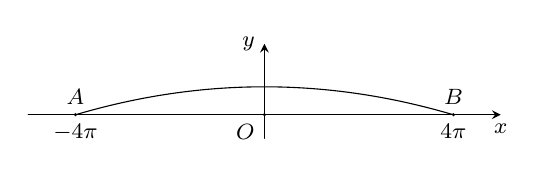
\begin{tikzpicture}[scale=0.6, font=\footnotesize, line join=round, line cap=round,>=stealth]
			\def\a{0} \def\b{-0.037} \def\c{0.59} % Hệ số
			\def\xmin{-5} \def\xmax{5}
			\def\ymin{-.5} \def\ymax{1.5}		
			\draw[->] (\xmin,0)--(\xmax,0) node [below]{$x$};
			\draw[->] (0,\ymin)--(0,\ymax) node [left]{$y$};
			\node at (0,0) [below left]{$O$};
			\fill (0,0)circle (1.0pt) (-4,0)node[above]{$A$} circle (1.0pt) (4,0)node[above]{$B$} circle (1.0pt) circle (1.0pt) (-4,0)node[below]{$-4\pi$} circle (1.0pt) (4,0)node[below]{$4\pi$} circle (1.0pt);
			\clip (-4,0) rectangle (4,1);
			\draw[smooth,samples=300] plot(\x,{\a*(\x)^4+\b*(\x)^2+\c});
	\end{tikzpicture}}
	\loigiai{
		Với mỗi điểm $ M $ nằm trên mặt cầu, khoảng cách từ điểm $ M $ đến mặt nước tương ứng với giá trị tung độ $ y $ của điểm $ M $,
		Xét phương trình $ 4{,}2\cdot \cos\dfrac{x}{8}=3\Leftrightarrow \cos \dfrac{x}{8}=\dfrac{5}{7}$.\\
		Do $ x\in [-4\pi;4\pi] $ nên $ \dfrac{x}{8}\in \left[-\dfrac{\pi}{2};\dfrac{\pi}{2} \right]  $.\\
		Khi đó, ta có $ \cos\dfrac{x}{8}=\dfrac{5}{7}\Leftrightarrow \dfrac{x}{8}\approx\pm 0{,}775 $, suy ra $ \left| \dfrac{x}{8}\right|<0{,}78\Leftrightarrow|x|<6{,}14$.\\
		Do sà lan có thể đi qua được gầm cầu nên chiều rộng của khối hàng hóa là $$ 2|x|<12{,}48<12{,}5. $$
	}
\end{bt}

\begin{bt}%[1D1V5-6]
% nguon: Archive/2024/TOAN_11_XE/TOAN_11_XE/data4/11C1/KNTT-1.4.tex #1093
 
	Một quả đạn pháo được bắn ra khỏi nòng pháo với vận tốc ban đầu $ v_0=500$ m/s hợp với phương ngang một góc $ \alpha $. Trong Vật lí, ta biết rằng, nếu bỏ qua sức cản của không khí và coi quả đạn pháo được bắn ra từ mặt đất thi quỹ đạo của quả đạn tuân theo phương trình $ y=\dfrac{-g}{2v_0^2\cos^2\alpha}\cdot x^2+x\tan \alpha $, ở đó $g = 10$ m/s$ ^2 $ là gia tốc trọng trường.
	\begin{listEX}[2]
		\item! Tính theo góc bắn $\alpha$ tầm xa mà quả đạn đạt tới (tức là khoảng cách từ vị trí bắn đến điểm quả đạn chạm đất).
		\item!Tìm góc bắn $ \alpha $ để quả đạn trúng mục tiêu cách vị trí đặt khẩu pháo $22~000$ (m).
	\end{listEX}
	\loigiai{
		\begin{listEX}[2]
			\item! Ta có \begin{eqnarray*}
				y=0&\Leftrightarrow& \dfrac{-g}{2v_0^2\cos^2\alpha}\cdot x^2+x\tan \alpha=0\\
				&\Leftrightarrow & x\left(\dfrac{-g}{2v_0^2\cos^2\alpha}\cdot x+\tan \alpha \right)=0 \\
				&\Leftrightarrow & \hoac{&x=0\\&x=\dfrac{v_0^2\sin2\alpha}{g}= 25~000\sin2\alpha.}
			\end{eqnarray*}
			Vậy tầm bay xa mà quả đạn đạt tới là $25~000\sin2\alpha$ (m).
			\item! Điều kiện $ 0\le\alpha\le \dfrac{\pi}{2}$\\Để quả đạn trúng mục tiêu cách vị trí đặt khẩu pháo $22~000$ (m) thì
			\begin{eqnarray*}
				25~000\sin2\alpha =22~000	& \Leftrightarrow & \sin 2\alpha =\dfrac{22}{25}\\
				&\Rightarrow & 2\alpha\approx 1{,}08 \Leftrightarrow \alpha \approx 0{,}54.	\end{eqnarray*}
			Vậy góc bắn khoảng $ 0{,}54 \text{ (rad) }\approx 30{,}82^\circ $ thì quả đạn trúng mục tiêu cách vị trí đặt khẩu pháo $22~000$ (m).
	\end{listEX}	}
\end{bt}

\begin{bt}%[1D1H5-4]
% nguon: Archive/2024/TOAN_11_XE/TOAN_11_XE/data4/11C1/KNTT-1.4.tex #1094
%[Tex hóa SGK 11, KNTT]
	Giải các phương trình sau:
	\begin{multicols}{2}
	\begin{enumerate}
		\item $\sin x=\dfrac{\sqrt{3}}{2}$.
		\item  $2\cos x=-\sqrt2$.
		\item $\sqrt3\tan\left(\dfrac{x}{2}+15^\circ \right)=1$.
		\item $\cot(2x-1)=\cot\dfrac{\pi}{5}$. 
	\end{enumerate}
	\end{multicols}
	\loigiai{
		\begin{enumerate}
			\item $\sin x=\dfrac{\sqrt{3}}{2}\Leftrightarrow \sin x=\sin\left( \dfrac{\pi}{3} \right) \Leftrightarrow \hoac{&x=\dfrac{\pi}{3}+k2\pi\\&x=\dfrac{2\pi}{3}+k2\pi}, k \in \mathbb{Z}$.
			\item $2\cos x=-\sqrt2 \Leftrightarrow \cos x=-\dfrac{\sqrt2}{2} \Leftrightarrow \cos x=\cos\left(\dfrac{3\pi}{4} \right)  \Leftrightarrow \hoac{&x=\dfrac{3\pi}{4}+k2\pi\\&x=-\dfrac{3\pi}{4}+k2\pi}, k \in \mathbb{Z}$.
			\item $\sqrt3\tan\left(\dfrac{x}{2}+15^\circ \right)=1 \Leftrightarrow \tan \left(\dfrac{x}{2}+15^\circ \right)=\dfrac{1}{\sqrt3} \Leftrightarrow \tan \left(\dfrac{x}{2}+15^\circ \right)=\tan\left(30^\circ \right) \\ \Leftrightarrow \dfrac{x}{2}+15^\circ=30^\circ+k180^{\circ} \Leftrightarrow x=30^\circ+k360^{\circ}, k \in \mathbb{Z}$.
			\item $\cot(2x-1)=\cot\dfrac{\pi}{5} \Leftrightarrow 2x-1=\dfrac{\pi}{5} +k\pi, x=\dfrac{1}{2}+\dfrac{\pi}{10}+\dfrac{k}{2}\pi, k \in \mathbb{Z}$.
		\end{enumerate}
	}
\end{bt}

\begin{bt}%[1D1V5-6]
% nguon: Archive/2024/TOAN_11_XE/TOAN_11_XE/data4/11C1/KNTT-1.4.tex #1095
%[Tex hóa SGK 11, KNTT]
	Một quả đạn pháo được bắn ra khỏi nòng pháo với vận tốc ban đầu $v_0=500 ~\mathrm{m} / \mathrm{s}$ hợp với phương ngang một góc $\alpha$. Trong Vật lí, ta biết rằng, nếu bỏ qua sức cản của không khí và coi quả đạn pháo được bắn ra từ mặt đất thì quỹ đạo của quả đạn tuân theo phương trình $y=\dfrac{-g}{2 v_0^2 \cos ^2 \alpha} x^2+x \tan \alpha$, ở đó $g=9{,}8 \mathrm{~m} / \mathrm{s}^2$ là gia tốc trọng trường.
	\begin{enumerate}[a)]
		\item Tính theo góc bắn $\alpha$ tầm xa mà quả đạn đạt tới (tức là khoảng cách từ vị trí bắn đến điểm quả đạn chạm đất).
		\item Tìm góc bắn $\alpha$ để quả đạn trúng mục tiêu cách vị trí đặt khẩu pháo $22000 \mathrm{~m}$.
		\item Tìm góc bắn $\alpha$ để quả đạn bay xa nhất.\end{enumerate}
	\loigiai{\begin{enumerate}[a)]
			\item Quả đạn chạm đất $\Rightarrow y=0$. Khi đó:\begin{center}
				$\dfrac{-g}{2 v_0^2 \cos ^2 \alpha} x^2+x \tan \alpha=0 \Leftrightarrow x\left(\dfrac{-g}{2 v_0^2 \cos ^2 \alpha} x+ \tan \alpha\right)=0\Rightarrow \hoac{&x=0\\&x=\dfrac{2 v_0^2 \cos ^2 \alpha.\tan \alpha}{g}}.$
			\end{center}
			Vậy tầm xa của quả đạn tính theo góc $\alpha$ là $x=\dfrac{2 v_0^2 \cos ^2 \alpha.\tan \alpha}{g}$.
			\item Để quả đạn trúng mục tiêu cách vị trí đặt khẩu pháo $22000 \mathrm{~m}$ thì
			\allowdisplaybreaks
			\begin{eqnarray*}
				&&\dfrac{2 v_0^2 \cos ^2 \alpha.\tan \alpha}{g}=22000 \\
				&\Leftrightarrow &	\dfrac{2. 500^2. \cos ^2 \alpha.\tan \alpha}{9,8}=22000 \\
				&\Leftrightarrow &\cos ^2 \alpha.\tan \alpha=0,4312.\\
				&\Leftrightarrow &\dfrac{1}{1+\tan^2\alpha}.\tan \alpha=0,4312.\\
				&\Leftrightarrow &0,4312\tan^2 \alpha-\tan\alpha+0,4312=0.\\
				&\Leftrightarrow &\hoac{&\tan\alpha=0{,}57\\&\tan\alpha=1{,}75}.\\
				&\Leftrightarrow &\hoac{&\alpha\approx 30^\circ +k180^\circ \\&\alpha\approx 60^\circ +k180^\circ}.
			\end{eqnarray*} Do góc $0<\alpha<90^\circ$ nên ta chọn $\alpha\approx 30^\circ$ hoặc $\alpha\approx 60^\circ$.
			\item Tầm  xa của quả đạn  là $x=\dfrac{2 v_0^2 \cos ^2 \alpha.\tan \alpha}{g}$, do đó quả đạn bay xa nhất khi $ \cos ^2 \alpha.\tan \alpha$ lớn nhất. Ta có: $\cos ^2 \alpha.\tan \alpha =\dfrac{\tan \alpha}{1+\tan^2\alpha}$.\\ Mặt khác $1+\tan^2\alpha \ge 2\tan\alpha$  nên ta có $\dfrac{\tan \alpha}{1+\tan^2\alpha} \le \dfrac{1}{2}$.\\  Dấu bằng xảy ra khi $\tan\alpha =1 \Leftrightarrow \alpha=45^\circ $ (do $0<\alpha<90^\circ$). \\
			Vậy khi góc bắn $\alpha=45^\circ$ thì quả đạn bay xa nhất.
			
	\end{enumerate}}
	
\end{bt}

\begin{bt}%[1D1H5-5]
% nguon: Archive/2024/TOAN_11_XE/TOAN_11_XE/data4/11C1/KNTT-1.4.tex #1101
%[TeX hóa SGK CTST]%[Trúc Danh]
	Giải các phương trình lượng giác sau
	\begin{multicols}{3}
		\begin{enumerate}
			\item $\sin 2x=\dfrac{1}{2}$.
			\item $\sin\left(x - \dfrac{\pi}{7}\right)=\sin\dfrac{2\pi}{7}$.
			\item $\sin 4x - \cos\left(x + \dfrac{\pi}{6}\right)=0$.
		\end{enumerate}
		
	\end{multicols}
	\loigiai{
		\begin{enumerate}
			\item \allowdisplaybreaks
			\begin{eqnarray*}
				&&\sin 2x=\dfrac{1}{2}\\
				&\Leftrightarrow& \sin 2x=\sin \dfrac{\pi}{6}\\
				&\Leftrightarrow& \hoac{&2x=\dfrac{\pi}{6}+k2\pi\\&2x=\dfrac{5\pi}{6}+k2\pi\\}\\
				&\Leftrightarrow& \hoac{&x=\dfrac{\pi}{12}+k\pi\\&x=\dfrac{5\pi}{12}+k\pi\\} (k\in \mathbb{Z}).
			\end{eqnarray*}
			\item \allowdisplaybreaks
			\begin{eqnarray*}
				&&\sin\left(x - \dfrac{\pi}{7}\right)=\sin\dfrac{2\pi}{7}\\
				&\Leftrightarrow& \hoac{& x - \dfrac{\pi}{7}=\dfrac{2\pi}{7} +k2\pi\\& x - \dfrac{\pi}{7}=\pi - \dfrac{2\pi}{7} +k2\pi\\}\\
				&\Leftrightarrow& \hoac{&x=\dfrac{3\pi}{7} + k2\pi\\&x=\dfrac{6\pi}{7} + k2\pi\\} (k\in\mathbb{Z}).
			\end{eqnarray*}
			\item \allowdisplaybreaks
			\begin{eqnarray*}
				&&\sin 4x - \cos\left(x + \dfrac{\pi}{6}\right)=0\\
				&\Leftrightarrow& \sin 4x = \cos\left(x + \dfrac{\pi}{6}\right)\\
				&\Leftrightarrow& \sin 4x = \sin \left(\dfrac{\pi}{3}-x\right)\\
				&\Leftrightarrow& \hoac{&4x=\dfrac{\pi}{3}-x+k2\pi\\&4x=\pi - \dfrac{\pi}{3}+x+k2\pi\\}\\
				&\Leftrightarrow& \hoac{&5x=\dfrac{\pi}{3}+k2\pi\\&3x= \dfrac{2\pi}{3}+k2\pi\\}\\
				&\Leftrightarrow& \hoac{&x=\dfrac{\pi}{15}+\dfrac{k2\pi}{5}\\&x= \dfrac{2\pi}{9}+\dfrac{k2\pi}{3}\\} (k\in \mathbb{Z}).
			\end{eqnarray*}
		\end{enumerate}
		
	}
\end{bt}

\begin{bt}%[1D1H5-5]
% nguon: Archive/2024/TOAN_11_XE/TOAN_11_XE/data4/11C1/KNTT-1.4.tex #1102
%[TeX hóa SGK CTST]%[Trúc Danh]
	Giải các phương trình lượng giác sau
	\begin{multicols}{3}
		\begin{enumerate}
			\item $\cos\left(x + \dfrac{\pi}{3}\right)=\dfrac{\sqrt{3}}{2}$.
			\item $\cos 4x=\cos\dfrac{5\pi}{12}$.
			\item $\cos^2x=1$.
		\end{enumerate}
	\end{multicols}
	\loigiai{
		\begin{enumerate}
			\item \allowdisplaybreaks
			\begin{eqnarray*}
				&&\cos\left(x + \dfrac{\pi}{3}\right)=\dfrac{\sqrt{3}}{2}\\
				&\Leftrightarrow &\cos\left(x + \dfrac{\pi}{3}\right)=\cos \dfrac{\pi}{6}\\
				&\Leftrightarrow & \hoac{&x + \dfrac{\pi}{3}=\dfrac{\pi}{6}+k2\pi\\&x + \dfrac{\pi}{3}=-\dfrac{\pi}{6}+k2\pi\\}\\
				&\Leftrightarrow &\hoac{&x=-\dfrac{\pi}{6}+k2\pi\\&x=-\dfrac{\pi}{2}+k2\pi\\} (k\in \mathbb{Z}).
			\end{eqnarray*}
			\item \allowdisplaybreaks
			\begin{eqnarray*}
				&&\cos 4x=\cos\dfrac{5\pi}{12}\\
				&\Leftrightarrow & \hoac{&4x=\dfrac{5\pi}{12}+k2\pi\\&4x=-\dfrac{5\pi}{12}+k2\pi\\}\\
				&\Leftrightarrow & \hoac{&x=\dfrac{5\pi}{48}+\dfrac{k\pi}{2}\\&4x=-\dfrac{5\pi}{48}+\dfrac{k\pi}{2}\\} (k\in \mathbb{Z}).
			\end{eqnarray*}
			\item \allowdisplaybreaks
			\begin{eqnarray*}
				&&\cos^2 x=1\\
				&\Leftrightarrow & \hoac{&\cos x=1\\&\cos x=-1\\}\\
				&\Leftrightarrow & \hoac{&x=k2\pi\\&x=\pi +k2\pi\\} (k\in\mathbb{Z}).			
			\end{eqnarray*}
		\end{enumerate}
		
	}
\end{bt}

\begin{bt}%[1D1H5-5]
% nguon: Archive/2024/TOAN_11_XE/TOAN_11_XE/data4/11C1/KNTT-1.4.tex #1103
%[TeX hóa SGK CTST]%[Trúc Danh]
	Giải các phương trình lượng giác sau
	\begin{multicols}{2}
		\begin{enumerate}
			\item $\tan x=\tan 55^{\circ}$.
			\item $\tan \left(2 x+\dfrac{\pi}{4}\right)=0$.
		\end{enumerate}
	\end{multicols}
	\loigiai{
		\begin{enumerate}
			\item $\tan x=\tan 55^{\circ}\Leftrightarrow x=55^{\circ} +k180^{\circ}$ $(k\in \mathbb{Z})$.
			\item $\tan \left(2 x+\dfrac{\pi}{4}\right)=0\Leftrightarrow 2x+\dfrac{\pi}{4}=k\pi\Leftrightarrow x=-\dfrac{\pi}{8}+\dfrac{k\pi}{2}$ $(k\in \mathbb{Z})$.
		\end{enumerate}
		
	}
\end{bt}

\begin{bt}%[1D1H5-3]
% nguon: Archive/2024/TOAN_11_XE/TOAN_11_XE/data4/11C1/KNTT-1.4.tex #1104
%[TeX hóa SGK CTST]%[Trúc Danh]
	Giải các phương trình lượng giác sau
	\begin{multicols}{2}
		\begin{enumerate}
			\item $\cot \left(\dfrac{1}{2} x+\dfrac{\pi}{4}\right)=-1$.
			\item $\cot 3 x=-\dfrac{\sqrt{3}}{3}$.
		\end{enumerate}
	\end{multicols}
	\loigiai{
		\begin{enumerate}
			\item \allowdisplaybreaks
			\begin{eqnarray*}
				&&\cot \left(\dfrac{1}{2} x+\dfrac{\pi}{4}\right)=-1\\
				&\Leftrightarrow& \dfrac{1}{2} x+\dfrac{\pi}{4}=-\dfrac{\pi}{4}+k\pi\\
				&\Leftrightarrow& x=-\pi+k2\pi\, (k\in \mathbb{Z}).
			\end{eqnarray*}
			\item \allowdisplaybreaks
			\begin{eqnarray*}
				&&\cot 3 x=-\dfrac{\sqrt{3}}{3}\\
				&\Leftrightarrow& \cot 3 x=\cot \left(-\dfrac{\pi}{3}\right)\\
				&\Leftrightarrow & 3x=-\dfrac{\pi}{3}+k\pi\\
				&\Leftrightarrow &x=-\dfrac{\pi}{9}+\dfrac{k\pi}{3} \, (k\in \mathbb{Z}).
			\end{eqnarray*}
		\end{enumerate}
		
	}
\end{bt}

\begin{bt}%[1D1H5-6]
% nguon: Archive/2024/TOAN_11_XE/TOAN_11_XE/data4/11C1/KNTT-1.4.tex #1106
%[TeX hóa SGK CTST]%[Trúc Danh]
	Trong hình dưới, ngọn đèn trên hải đăng $H$ cách bờ biển $y y'$ một khoảng $HO=1$ km. Đèn xoay ngược chiều kim đồng hồ với tốc độ $\dfrac{\pi}{10}$ rad/s và chiếu hai luồng ánh sáng về hai phía đối diện nhau. Khi đèn xoay, điểm $M$ mà luồng ánh sáng của hải đăng rọi vào bờ biển chuyển động dọc theo bờ.
	\begin{flushright}
		\textit{(Theo https://www:mnhs.org/splitrock/learn/technology)}
	\end{flushright}
	\begin{center}
		
\begin{tikzpicture}[scale=1.3,font=\footnotesize, line join=round, line cap=round, >=stealth]
			\definecolor{nen tron}{RGB}{173,223,246}
			\definecolor{thap trai}{rgb}{0.51, 0.21, 0.21}
			\definecolor{thap mat}{rgb}{0.51, 0.21, 0.30}
			\definecolor{luon duoi}{RGB}{1,116,181}
			\fill[black!40] (-2.5,-2.3) rectangle (2.5,3.2);
			% NữaTháp phải
			\fill[black!20] (0,-1.7) ellipse (2 and .5); 
			\def \A{
				(0,2)
				..controls +(-90:.1) and +(150:.12)..(.07,1.46)
				..controls +(-60:.1) and +(90:.1)..(.11,1.32)
				--(.52,1.11)--(.52,1.08)--(.4,1.08)--(.4,.72)--(.48,.72)--(.48,.6)--(.4,.6)
				--(.6,-1.49)--(0,-1.49)--(0,2)}
			\fill[thap mat] \A;
			\fill[thap trai][xscale=-1] \A;
			% Ô cửa phải
			\def\B{
				(.11,.76)--(.26,.76)--(.26,1.04)--(.11,1.04)--(.11,.76) 
				(0,.76)--(.07,.76)--(.07,1.04)--(0,1.04)--(0,.76)}
			\fill[nen tron]\B;
			\fill[nen tron][xscale=-1] \B;
			% chân tháp
			\fill[thap mat] 
			(0,-1.49)--(.7,-1.49)--(.72,-1.6)--(0,-1.6);
			\fill[thap trai]
			(0,-1.49)--(0,-1.6)
			..controls +(175:.3) and +(3:.1)..(-.72,-1.58) --(-.71,-1.49)
			--(0,-1.49);
			
			\foreach \a in {0, 20, ..., 360}{%
				\begin{scope}[shift={(0,1.8)}]
					\fill[rotate=\a,white] (0,0)--(0,1);
					\fill[rotate=45,white] (-1.5,0)--(0,0.03)--(1.5,0)--(0,-0.03)--(-1.5,0);
				\end{scope}
			}
			\fill [white] (0,1.8) circle (.2);
			
		\end{tikzpicture} \hspace{2cm}
		\begin{tikzpicture}[scale=1,font=\footnotesize, line join=round, line cap=round, >=stealth]
			\path 
			(0,0) coordinate (O)
			(-3,0) coordinate (H)
			(0,2) coordinate (M)
			(0,-3) coordinate (N)
			
			;
			
			\draw[->] (0,-4) -- (0,3)node[right] {$y$};
			\draw[blue,shorten >=-2cm] (M)--(H);
			\draw[dashed] (H)--(O);
			\draw pic[draw, angle radius=2mm]{right angle=H--O--M};
			\pic[draw,"$\alpha$", angle eccentricity=0.6,angle radius=0.8cm]{angle=O--H--M};
			\path (O)--(N) node[right,midway]{$1$ km};
			\path (O)--(H) node[below,midway]{$1$ km};
			\path (0,-4) node[left]{$y'$};
			\path (0,-4) node[right]{bờ biển};
			\foreach \x/\g in {H/90,O/0,N/0,M/0} \fill[black] (\x) circle (1pt)+(\g:.3) node {$\x$};
			%%\path ([xshift=-.25cm]current bounding box.south) node[below]{\hinhve};
		\end{tikzpicture}
	\end{center}
	\begin{enumerate}
		\item Ban đầu luồng sáng trùng với đường thẳng $HO$. Viết hàm số biểu thị toạ độ $y_M$ của điểm $M$ trên trục $Oy$ theo thời gian $t$.
		\item Ngôi nhà $N$ nằm trên bờ biển với toạ độ $y_N=-1$ (km). Xác định các thời điểm $t$ mà đèn hải đăng chiếu vào ngôi nhà.
	\end{enumerate}
	\loigiai{
		\begin{enumerate}
			\item Xét $\triangle OMH$ có 
			$OM=OH\cdot \tan \alpha\Rightarrow y_M=\tan \alpha=\tan \left(\dfrac{\pi t}{10}\right)$.\\
			Vậy hàm số biểu thị toạ độ $y_M$ của điểm $M$ trên trục $Oy$ theo thời gian $t$ là $y_M=\tan \left(\dfrac{\pi t}{10}\right)$.
			\item Theo giả thiết, ta có \allowdisplaybreaks
			\begin{eqnarray*}
				&&y_N=-1\\
				&\Leftrightarrow& \tan \left(\dfrac{\pi t}{10}\right)=-1\\
				&\Leftrightarrow& \dfrac{\pi t}{10}=-\dfrac{\pi}{4}+k\pi\\ &\Leftrightarrow&  t=-\dfrac{5}{2}+10k \,(k\in \mathbb{N}^*).
			\end{eqnarray*}
		\end{enumerate}
		
	}
\end{bt}

\begin{bt}%[1D1H3-2]
% nguon: Archive/2024/TOAN_11_XE/TOAN_11_XE/data4/11C1/KNTT-1.OTC.tex #1107
%[Tex hóa SGK CD-CT,T12/22, TVN-006]
Cho góc $\alpha$ thỏa mãn $\dfrac{\pi}{2}<\alpha<\pi$, $\cos \alpha=-\dfrac{1}{\sqrt{3}}$. Tính giá trị của các biểu thức sau
\begin{multicols}{2}
\begin{enumerate}
	\item $\sin \left(\alpha+\dfrac{\pi}{6}\right)$;
	\item $\cos\left(\alpha+\dfrac{\pi}{6}\right)$;
	\item $\sin\left(\alpha-\dfrac{\pi}{6}\right)$;
	\item $\cos\left(\alpha-\dfrac{\pi}{6}\right)$.
\end{enumerate}
\end{multicols}
\loigiai{
Do $\dfrac{\pi}{2}<\alpha<\pi$ nên $\heva{&\cos\alpha <0\\&\sin\alpha >0.}$\\
Khi đó $\sin \alpha=\sqrt{1-\cos^2\alpha}=\sqrt{1-\left(-\dfrac{1}{\sqrt{3}}\right)^2}=\dfrac{\sqrt{6}}{3}$.
\begin{enumerate}
	\item Ta có $\sin\left(\alpha+\dfrac{\pi}{6}\right)=\sin\alpha\cos\dfrac{\pi}{6}+\cos\alpha\sin\dfrac{\pi}{6}=\dfrac{\sqrt{6}}{3}\cdot \dfrac{\sqrt{3}}{2}-\dfrac{1}{\sqrt{3}}\cdot \dfrac{1}{2}=\dfrac{3\sqrt{2}-\sqrt{3}}{6}$.
	\item Ta có $\cos\left(\alpha+\dfrac{\pi}{6}\right)=\cos\alpha\cos\dfrac{\pi}{6}-\sin\alpha\sin\dfrac{\pi}{6}=-\dfrac{1}{\sqrt{3}}\cdot \dfrac{\sqrt{3}}{2}-\dfrac{\sqrt{6}}{3}\cdot \dfrac{1}{2}=\dfrac{-3-\sqrt{6}}{6}$.
	\item Ta có $\sin\left(\alpha-\dfrac{\pi}{6}\right)=\sin\alpha\cos\dfrac{\pi}{6}-\cos\alpha\sin\dfrac{\pi}{6}=\dfrac{\sqrt{6}}{3}\cdot \dfrac{\sqrt{3}}{2}+\dfrac{1}{\sqrt{3}}\cdot \dfrac{1}{2}=\dfrac{3\sqrt{2}+\sqrt{3}}{6}$.
	\item Ta có $\cos\left(\alpha-\dfrac{\pi}{6}\right)=\cos\alpha\cos\dfrac{\pi}{6}+\sin\alpha\sin\dfrac{\pi}{6}=-\dfrac{1}{\sqrt{3}}\cdot \dfrac{\sqrt{3}}{2}+\dfrac{\sqrt{6}}{3}\cdot \dfrac{1}{2}=\dfrac{-3+\sqrt{6}}{6}$.
\end{enumerate}
}
\end{bt}

\begin{bt}%[1D1H3-3]
% nguon: Archive/2024/TOAN_11_XE/TOAN_11_XE/data4/11C1/KNTT-1.OTC.tex #1108

Cho bất kì góc $\alpha$. Chứng minh các đẳng thức sau
\begin{multicols}{2}
	\begin{enumerate}
		\item $\left(\sin \alpha+\cos\alpha\right)^2=1+\sin 2\alpha$;
		\item $\cos^4\alpha-\sin^4\alpha=\cos 2\alpha$.
	\end{enumerate}
\end{multicols}
\loigiai{
\begin{enumerate}
	\item $\left(\sin \alpha+\cos\alpha\right)^2=\sin^2\alpha+2\sin\alpha\cos\alpha+\cos^2\alpha=1+\sin 2\alpha$;
	\item $\cos^4\alpha-\sin^4\alpha=\left(\cos^2\alpha-\sin^2\alpha\right)\left(\cos^2\alpha+\sin^2\alpha\right)=\cos 2\alpha$.
\end{enumerate}
}
\end{bt}

\begin{bt}%[1D1H4-6]
% nguon: Archive/2024/TOAN_11_XE/TOAN_11_XE/data4/11C1/KNTT-1.OTC.tex #1109

Tìm tập giá trị của các hàm số sau
\begin{multicols}{2}
\begin{enumerate}
	\item $y=2\cos\left(2x-\dfrac{\pi}{3}\right)-1$;
	\item $y=\sin x+\cos x$.
\end{enumerate}
\end{multicols}
\loigiai{
\begin{enumerate}
	\item Tập xác định $\mathscr{D}=\mathbb{R}$.\\
	Ta có
	\allowdisplaybreaks
	\begin{eqnarray*}
 &&-1\le \cos\left(2x-\dfrac{\pi}{3}\right)\le 1\\
 &\Leftrightarrow&-2\le 2\cos\left(2x-\dfrac{\pi}{3}\right)\le 2\\
 &\Leftrightarrow&-3\le 2\cos\left(2x-\dfrac{\pi}{3}\right)-1\le 1.	
	\end{eqnarray*}	
Vậy $\min y=-3$ khi và chỉ khi $\cos\left(2x-\dfrac{\pi}{3}\right)=-1\Leftrightarrow 2x-\dfrac{\pi}{3}=\pi+k2\pi\Leftrightarrow x=\dfrac{2\pi}{3}+k\pi$ với $k\in\mathbb{Z}$.\\
$\max y=1$ khi và chỉ khi $\cos\left(2x-\dfrac{\pi}{3}\right)=1\Leftrightarrow 2x-\dfrac{\pi}{3}=k2\pi\Leftrightarrow x=\dfrac{\pi}{6}+k\pi$ với $k\in\mathbb{Z}$.\\
Vậy tập giá trị của hàm số là $[-3;1]$.
	\item Tập xác định $\mathscr{D}=\mathbb{R}$.\\
	Ta có $\sin x+\cos x=\sqrt{2}\left(\sin x\dfrac{\sqrt{2}}{2}+\cos x\dfrac{\sqrt{2}}{2}\right)=\sqrt{2}\sin\left(x+\dfrac{\pi}{4}\right)$.\\
	Khi đó 
	\allowdisplaybreaks
	\begin{eqnarray*}
		&&-1\le \sin\left(x+\dfrac{\pi}{4}\right)\le 1\\
		&\Leftrightarrow&-\sqrt{2}\le\sqrt{2}\sin\left(x+\dfrac{\pi}{4}\right)\le \sqrt{2}.
	\end{eqnarray*}
Vậy $\min y=-\sqrt{2}$ khi và chỉ khi $\sin\left(x+\dfrac{\pi}{4}\right)=-1\Leftrightarrow x+\dfrac{\pi}{4}=-\dfrac{\pi}{2}+k2\pi\Leftrightarrow x=-\dfrac{3\pi}{4}+k2\pi$ với $k\in\mathbb{Z}$.\\
$\max y=\sqrt{2}$ khi và chỉ khi $\sin\left(x+\dfrac{\pi}{4}\right)=1\Leftrightarrow x+\dfrac{\pi}{4}=\dfrac{\pi}{2}+k2\pi\Leftrightarrow x=\dfrac{\pi}{4}+k2\pi$ với $k\in\mathbb{Z}$. \\
Vậy tập giá trị của hàm số là $\left[-\sqrt{2};\sqrt{2}\right]$.
\end{enumerate}
}
\end{bt}

\begin{bt}%[1D1H5-5]
% nguon: Archive/2024/TOAN_11_XE/TOAN_11_XE/data4/11C1/KNTT-1.OTC.tex #1110

Giải các phương trình sau
\begin{multicols}{3}
\begin{enumerate}
	\item $\cos\left(3x-\dfrac{\pi}{4}\right)=-\dfrac{\sqrt{2}}{2}$;
	\item $2\sin^2x-1+\cos 3x=0$;
	\item $\tan\left(2x+\dfrac{\pi}{5}\right)=\tan\left(x-\dfrac{\pi}{6}\right)$.
\end{enumerate}
\end{multicols}
\loigiai{
\begin{enumerate}
	\item Ta có
	\allowdisplaybreaks
	\begin{eqnarray*}
		\cos\left(3x-\dfrac{\pi}{4}\right)=-\dfrac{\sqrt{2}}{2}&\Leftrightarrow&\hoac{&3x-\dfrac{\pi}{4}=\dfrac{3\pi}{4}+k2\pi\\&3x-\dfrac{\pi}{4}=-\dfrac{3\pi}{4}+k2\pi}\\
		&\Leftrightarrow&\hoac{&3x=\pi+k2\pi\\&3x=-\dfrac{\pi}{2}+k2\pi}\\
		&\Leftrightarrow&\hoac{&x=\dfrac{\pi}{3}+\dfrac{k2\pi}{3}\\&x=-\dfrac{\pi}{6}+\dfrac{k2\pi}{3}},\left(k\in\mathbb{Z}\right).
	\end{eqnarray*}
	\item Ta có
	\allowdisplaybreaks
	\begin{eqnarray*}
		2\sin^2x-1+\cos 3x=0&\Leftrightarrow&\cos 3x-\cos 2x=0\\
		&\Leftrightarrow&\cos 3x=\cos 2x\\
		&\Leftrightarrow&\hoac{&3x=2x+k2\pi\\&3x=-2x+k2\pi}\\
		&\Leftrightarrow&\hoac{&x=k2\pi\\&5x=k2\pi}\\
		&\Leftrightarrow&\hoac{&x=k2\pi\\&x=\dfrac{k2\pi}{5}},\left(k\in\mathbb{Z}\right).
	\end{eqnarray*}
	\item Ta có
	\allowdisplaybreaks
	\begin{eqnarray*}
	\tan\left(2x+\dfrac{\pi}{5}\right)=\tan\left(x-\dfrac{\pi}{6}\right)&\Leftrightarrow&\heva{&x-\dfrac{\pi}{6}\ne\dfrac{\pi}{2}+k\pi\\&2x+\dfrac{\pi}{5}\ne\dfrac{\pi}{2}+k\pi\\&2x+\dfrac{\pi}{5}=x-\dfrac{\pi}{6}+k\pi}\\
	&\Leftrightarrow&\heva{&x\ne\dfrac{2\pi}{3}+k\pi\\&x\ne\dfrac{\pi}{20}+\dfrac{k\pi}{2}\\&x=-\dfrac{11\pi}{30}+k\pi},\left(k\in\mathbb{Z}\right).	
	\end{eqnarray*}
Vậy nghiệm của phương trình là $x=-\dfrac{11\pi}{30}+k\pi$ với $k\in\mathbb{Z}$.
\end{enumerate}
}
\end{bt}

\begin{bt}%[1D1H4-8]
% nguon: Archive/2024/TOAN_11_XE/TOAN_11_XE/data4/11C1/KNTT-1.OTC.tex #1111
%[Tex hóa SGK CD-CT,T12/22, TVN-006]
Huyết áp là áp lực cần thiết tác động lên thành của động mạch để đưa máu từ tim đến nuôi dưỡng các mô trong cơ thể. Huyết áp được tạo ra do lực co bóp của cơ tim và sức cản của thành động mạch. Mỗi lần tim đập, huyết áp của chúng ta tăng rồi giảm giữa các nhịp. Huyết áp tối đa và huyết áp tối thiểu được gọi tương ứng là huyết áp tâm thu và tâm trương. Chỉ số huyết áp của chúng ta được viết là huyết áp tâm thu/ huyết áp tâm trương. Chỉ số huyết áp $120/80$ là bình thường. Giả sử huyết áp của một người nào đó được mô hình hóa bởi hàm số
$$p(t)=115+25\sin(160\pi t)$$
trong đó $p(t)$ là huyết áp tính theo đơn vị mmHg (milimet thủy ngân) và thời gian $t$ tính theo phút.
\begin{enumerate}
	\item Tìm chu kì của hàm số $p(t)$.
	\item Tìm số nhịp tim mỗi phút.
	\item Tìm số chỉ huyết áp. So sánh huyết áp của người này với huyết áp bình thường.
\end{enumerate}
\loigiai{
\begin{enumerate}
	\item Chu kì của hàm số $p(t)$ là $T=\dfrac{2\pi}{160\pi}=\dfrac{1}{80}$.
	\item Chu kì của huyết áp là $T=\dfrac{1}{80}$ nghĩa là $1$ phút thì nhịp tim của người này là $80$.
	\item Ta có
	\allowdisplaybreaks
	\begin{eqnarray*}
		&&-1\le \sin(160\pi t)\le 1\\
		&\Leftrightarrow& -25\le 25\sin(160\pi t)\le 25\\
		&\Leftrightarrow& 90\le 115+25\sin(160\pi t)\le 140.
	\end{eqnarray*}
Do đó, số chỉ huyết áp của người này là $140/90$. Huyết áp của người này so với huyết áp bình thường là cao hơn.
\end{enumerate}
}
\end{bt}

\begin{bt}%[1D1H2-5]
% nguon: Archive/2024/TOAN_11_XE/TOAN_11_XE/data4/11C1/KNTT-1.OTC.tex #1112
%[Tex hóa SGK CD-CT,T12/22, TVN-006]
\immini{
Khi một tia sáng truyền từ không khí vào mặt nước thì một phần tia sáng bị phản xạ trên bề mặt, phần còn lại bị khúc xạ như hình bên. Góc tới $i$ liên hệ với góc khúc xạ $r$ bởi Định luật khúc xạ ánh sáng
$$\dfrac{\sin i}{\sin r}=\dfrac{n_2}{n_1}.$$
Ở đây, $n_1$ và $n_2$ tương ứng với chiết suất của môi trường $1$ (không khí) và môi trường $2$ (nước). Cho biết góc tới $i=50^\circ$, hãy tính góc khúc xạ, biết rằng chiết suất của không khí bằng $1$ còn chiết suất của nước là $1{,}33$.
}
{
	\begin{tikzpicture}[>=stealth,line join=round,line cap=round,font=\footnotesize,scale=.7]
	\path
	(0,0)coordinate(I)++(90:3)coordinate(N)++(-90:6)coordinate(N')
	(I)++(0:3)coordinate(B)++(180:6)coordinate(A)
	(I)++(30:3)coordinate(S')
	(I)++(150:3)coordinate(S)
	(I)++(-55:3)coordinate(R)
	;
	\fill[cyan!20!](-3,-3)rectangle(3,0)
	;
	\draw (A)--(B)
	;
	\draw[dashed](N)--(N')
	;
	\draw[->,midway](S)--(I)
	;
	\draw[->](I)--(S')
	;
	\draw[->](I)--(R)
	;
	\foreach \p/\r in {N/180,N'/180,S/160,S'/90,R/0,I/-135}
	\fill (\p) node[shift={(\r:3mm)}]{$\p$}
	;
	\draw pic[angle radius=3mm,draw=red,fill=green!50,"$i$",angle eccentricity=1.5] {angle = N--I--S}
	;
	\draw pic[angle radius=4mm,draw=orange,fill=orange!50,"$i'$",angle eccentricity=1.5] {angle = S'--I--N}
	;
	\draw pic[angle radius=4mm,draw=blue,fill=blue!50,"$r$",angle eccentricity=1.5] {angle = N'--I--R}
	;
	\draw (-2.5,.5)circle(7pt)node{$1$}
		(-2.5,-.5)circle(8pt)node{$2$}
		;	
\end{tikzpicture}
}
\loigiai{
Ta có $\dfrac{\sin i}{\sin r}=\dfrac{n_2}{n_1}\Leftrightarrow \dfrac{\sin 50^\circ}{\sin r}=\dfrac{1{,}33}{1}\Leftrightarrow \sin r=\dfrac{\sin 50^\circ}{1{,}33}\Rightarrow r\approx 35{,}17^\circ$.
}
\end{bt}

\begin{bt}%[1D1H1-6]
% nguon: Archive/2024/TOAN_11_XE/TOAN_11_XE/data4/11C1/KNTT-1.OTC.tex #1113
%[Trần Công Duy]
	Một chiếc quạt trần năm cánh quay với tốc độ 45 vòng trong một phút. Chọn chiều quay của quạt là chiều thuận. Sau 3 giây, quạt quay được một góc có số đo bao nhiêu radian?
	\loigiai{
		Trong 3 giây, số vòng quạt quay được là: $\dfrac{3}{60}\cdot 45=2{,}25$. \\
		Suy ra, góc quay có số đo là: $2{,}25\cdot 2\pi=4{,}5$ (rad).
	}
\end{bt}

\begin{bt}%[1D1H3-5]
% nguon: Archive/2024/TOAN_11_XE/TOAN_11_XE/data4/11C1/KNTT-1.OTC.tex #1114
%[Trần Công Duy]
	Cho $\cos \alpha=\dfrac{1}{3}$ và $-\dfrac{\pi}{2}<\alpha<0$. Tính:
	\begin{listEX}[3]
		\item $\sin \alpha$;
		\item $\sin 2 \alpha$;
		\item $\cos \left(\alpha+\dfrac{\pi}{3}\right)$.
	\end{listEX}
	\loigiai{
		\begin{listEX}
			\item Ta có $\sin^2\alpha+\cos^2\alpha=1\Rightarrow \sin^2\alpha=1-\cos^2\alpha=1-\left(\dfrac{1}{3}\right)^2=\dfrac{8}{9}\Rightarrow \sin\alpha=\pm \dfrac{2\sqrt{2}}{3}$.\\
			Mặt khác, $-\dfrac{\pi}{2}<\alpha<0$ nên $\sin\alpha<0$. Do đó $\sin\alpha=-\dfrac{2\sqrt{2}}{3}$.
			\item Ta có $\sin 2 \alpha=2\sin\alpha\cos\alpha=2\cdot \dfrac{-2\sqrt{2}}{3}\cdot \dfrac{1}{3}=-\dfrac{4\sqrt{2}}{9}$.
			\item $\cos \left(\alpha+\dfrac{\pi}{3}\right)=\cos\alpha\cos\dfrac{\pi}{3}-\sin\alpha\sin\dfrac{\pi}{3}=\dfrac{1}{3}\cdot \dfrac{1}{2}-\dfrac{-2\sqrt{2}}{3}\cdot \dfrac{\sqrt{3}}{2}=\dfrac{1+2\sqrt{6}}{6}$.
		\end{listEX}
	}
\end{bt}

\begin{bt}%[1D1V3-4]
% nguon: Archive/2024/TOAN_11_XE/TOAN_11_XE/data4/11C1/KNTT-1.OTC.tex #1115
%[Trần Công Duy]
	Chứng minh đẳng thức lượng giác:
	\begin{listEX}[2]
		\item $\sin (\alpha+\beta) \sin (\alpha-\beta)=\sin ^2 \alpha-\sin ^2 \beta$;
		\item $\cos ^4 \alpha-\cos ^4\left(\alpha-\dfrac{\pi}{2}\right)=\cos 2 \alpha$.
	\end{listEX}
	\loigiai{
		\begin{listEX}
			\item Ta có 
			\allowdisplaybreaks
			\begin{eqnarray*}
				\sin (\alpha+\beta)&=&\sin\alpha\cos\beta+\cos\alpha\sin\beta\\
				\sin (\alpha-\beta)&=&\sin\alpha\cos\beta-\cos\alpha\sin\beta\\
				\Rightarrow \sin (\alpha+\beta) \sin (\alpha-\beta)&=&(\sin\alpha\cos\beta+\cos\alpha\sin\beta)(\sin\alpha\cos\beta-\cos\alpha\sin\beta)\\
				&=& \sin^2\alpha\cos^2\beta+\cos^2\alpha\sin^2\beta\\
				&=&\sin^2\alpha\left(1-\sin^2\beta\right)+\left(1-\sin^2\alpha\right)\sin^2\beta\\
				&=&\sin^2\alpha-\sin^2\beta.
			\end{eqnarray*}	
			\item Ta có
			\allowdisplaybreaks
			\begin{eqnarray*}
				&&\cos ^4 \alpha-\cos ^4\left(\alpha-\dfrac{\pi}{2}\right)\\
				&=&\cos^4\alpha-\cos^4\left(\dfrac{\pi}{2}-\alpha\right)\\
				&=&\cos^4\alpha-\sin^4\alpha \\
				&=&\left(\cos^2\alpha-\sin^2\alpha\right)\left(\cos^2\alpha+\sin^2\alpha\right)\\
				&=&\cos^2\alpha-\sin^2\alpha=\cos 2\alpha.
			\end{eqnarray*}	
		\end{listEX}
	}
\end{bt}

\begin{bt}%[1D1H5-5]
% nguon: Archive/2024/TOAN_11_XE/TOAN_11_XE/data4/11C1/KNTT-1.OTC.tex #1116
%[Trần Công Duy]
	Nghiệm dương nhỏ nhất của phương trình $\sin \left(x+\dfrac{\pi}{6}\right)-\sin 2 x=0$ là bao nhiêu?
	\loigiai{
		\allowdisplaybreaks
		\begin{eqnarray*}
			&&\sin \left(x+\dfrac{\pi}{6}\right)-\sin 2 x=0\\
			&\Leftrightarrow& \sin 2x=\sin \left(x+\dfrac{\pi}{6}\right) \\
			&\Leftrightarrow& \hoac{&2x=x+\dfrac{\pi}{6}+k2\pi\\&2x=\pi-x-\dfrac{\pi}{6}+k2\pi}
			\Leftrightarrow \hoac{&x=\dfrac{\pi}{6}+k2\pi\\&x=\dfrac{5\pi}{18}+\dfrac{k2\pi}{3}} (k\in\mathbb{Z}).
		\end{eqnarray*}	
		Ta thấy nghiệm dương nhỏ nhất của họ $x=\dfrac{\pi}{6}+k2\pi$ là $x=\dfrac{\pi}{6}$ (ứng với $k=0$); nghiệm dương nhỏ nhất của họ nghiệm $x=\dfrac{5\pi}{18}+\dfrac{k2\pi}{3}$ là $x=\dfrac{5\pi}{18}$ (ứng với $k=0$). Suy ra nghiệm dương nhỏ nhất của phương trình lượng giác đã cho là $x=\dfrac{\pi}{6}$. 
	}
\end{bt}

\begin{bt}%[1D1V5-5]
% nguon: Archive/2024/TOAN_11_XE/TOAN_11_XE/data4/11C1/KNTT-1.OTC.tex #1117
%[Trần Công Duy]
	Giải các phương trình sau:
	\begin{listEX}[3]
		\item $\sin 2 x+\cos 3 x=0$
		\item $\sin x \cos x=\dfrac{\sqrt{2}}{4}$;
		\item $\sin x+\sin 2 x=0$.
	\end{listEX}
	\loigiai{
		\begin{listEX}
			\item $\sin 2 x+\cos 3x=0$
			\allowdisplaybreaks
			\begin{eqnarray*}
				\sin 2x+\cos 3x=0 &\Leftrightarrow& \cos 3x=-\sin 2x \\
				&\Leftrightarrow& \cos 3x=\sin \left(-2x\right)\\
				&\Leftrightarrow& \cos 3x=\cos \left(\dfrac{\pi}{2}+2x\right)\\
				&\Leftrightarrow&\hoac{&3x=\dfrac{\pi}{2}+2x+k2\pi\\&3x=-\dfrac{\pi}{2}-2x+k2\pi}\Leftrightarrow\hoac{&x=\dfrac{\pi}{2}+k2\pi\\&x=-\dfrac{\pi}{10}+\dfrac{k2\pi}{5}} (k\in\mathbb{Z}).
			\end{eqnarray*}	
			Vậy phương trình có các nghiệm là $x=\dfrac{\pi}{2}+k2\pi, k\in\mathbb{Z}$ và $x=-\dfrac{\pi}{10}+\dfrac{k2\pi}{5}, k\in\mathbb{Z}$.
			\item $\sin x \cos x=\dfrac{\sqrt{2}}{4}$;
			\allowdisplaybreaks
			\begin{eqnarray*}
				&&\sin x \cos x=\dfrac{\sqrt{2}}{4} \\
				&\Leftrightarrow& 2\sin x\cos x=\dfrac{\sqrt{2}}{2}\\
				&\Leftrightarrow&\sin 2x=\dfrac{\sqrt{2}}{2}=\sin \dfrac{\pi}{4} \\
				&\Leftrightarrow& \hoac{&2x=\dfrac{\pi}{4}+k2\pi\\&2x=\pi-\dfrac{\pi}{4}+k2\pi} 
				\Leftrightarrow\hoac{&x=\dfrac{\pi}{8}+k\pi\\&x=\dfrac{3\pi}{8}+k\pi} (k\in\mathbb{Z}).
			\end{eqnarray*}	
			Vậy phương trình có các nghiệm là $x=\dfrac{\pi}{8}+k\pi, k\in\mathbb{Z}$ và $x=\dfrac{3\pi}{8}+k\pi, k\in\mathbb{Z}$.
			\item $\sin x+\sin 2 x=0$.
			\allowdisplaybreaks
			\begin{eqnarray*}
				&&\sin x+\sin 2 x=0 \\
				&\Leftrightarrow& \sin x+2\sin x\cos x=0 \\
				&\Leftrightarrow& \sin x \left(1+2\cos x\right)=0 \\
				&\Leftrightarrow& \hoac{&\sin x=0\\&1+2\cos x=0} \\
				&\Leftrightarrow& \hoac{&\sin x=0\\&\cos x=-\dfrac{1}{2}}\Leftrightarrow \hoac{&x=k\pi\\&x=\pm \dfrac{2\pi}{3}+k2\pi} (k\in\mathbb{Z}).
			\end{eqnarray*}	
			Vậy phương trình có các nghiệm là $k\pi, k\in\mathbb{Z}$ và $x=\pm \dfrac{2\pi}{3}+k2\pi, k\in\mathbb{Z}$.
		\end{listEX}
	}
\end{bt}

\begin{bt}%[1D1V5-6]
% nguon: Archive/2024/TOAN_11_XE/TOAN_11_XE/data4/11C1/KNTT-1.OTC.tex #1118
%[Trần Công Duy]
	Độ sâu $h(\mathrm{~m})$ của mực nước ở một cảng biển vào thời điểm $t$ (giờ) sau khi thuỷ triều lên lần đầu tiên trong ngày được tính xấp xỉ bởi công thức $h(t)=0{,}8 \cos 0{,}5 t+4$.\\
	\mbox{}\hfill (Theo \textit{https://noc.ac.uk/files/documents/ business/an-introduction-to-tidalmodelling.pdf})
	\begin{listEX}
		\item Độ sâu của nước vào thời điểm $t=2$ là bao nhiêu mét?
		\item Một con tàu cần mực nước sâu tối thiểu $3{,}6 \mathrm{~m}$ đề có thể di chuyển ra vào cảng an toàn. Dựa vào đồ thị của hàm số côsin, hãy cho biết trong vòng $12$ tiếng sau khi thuỷ triều lên lần đầu tiên, ở những thời điểm $t$ nào tàu có thể hạ thuỷ. Làm tròn kết quả đến hàng phần trăm.
	\end{listEX}
	\loigiai{
		\begin{listEX}
			\item Với $t=2$ thì $h(2)=0,8 \cos 0{,}5\cdot 2+4=0,8 \cos 1+4\approx 4{,}43$ (m).
			\item Tàu có thể hạ thủy vào những thời điểm $t$ thỏa mãn
			\allowdisplaybreaks
			\begin{eqnarray*}
				0{,}8 \cos 0{,}5 t+4 \geq 3{,}6 \Leftrightarrow \cos 0{,}5 t \geq -\dfrac{1}{2}.\quad (*)
			\end{eqnarray*}	
			Đặt $0{,}5t=x$. Với $t\in[0;12]$ thì $x\in [0;6]$. Khi bất phương trình $(*)$ trở thành $\cos x\geq -\dfrac{1}{2}$. 
			\\
			Quan sát đồ thị hàm số $y=f(x)=\cos x$ trên $[0;6]$:
			\begin{center}
				\begin{tikzpicture}[line cap=butt,line join=miter,>=stealth]
					\tikzset{declare function={xmin=-.5;xmax=7;ymin=-1.5;ymax=2;},
						smooth,samples=100
					}
					\draw[->] (xmin,0)--(xmax,0) node[shift={(-100:7pt)},font=\normalsize]{$ x $};
					\draw[->] (0,ymin)--(0,ymax) node[shift={(190:7pt)},font=\normalsize]{$ y $};
					\fill (0,0) node[shift={(135:7pt)},font=\normalsize]{$ O $};
					\clip (xmin,ymin) rectangle (xmax,ymax);
					\draw[thick]  plot[domain=0:xmax] (\x, -.5);
					\draw[thick] plot[domain=0:6] (\x,{cos(\x r)});
					\draw[dashed] (2*pi/3,0)--++(0,-.5) 
					(4*pi/3,0)--++(0,-.5)
					(pi,0)--++(0,-1)--++(-pi,0)node[left]{$-1$}
					(6,0)node[below,font=\normalsize]{$6$}--++(0,.96017)
					(0,1)node[left,font=\normalsize]{$1$}
					(6.3,-.8)node[font=\normalsize]{$y=-\tfrac{1}{2}$}
					;
					\foreach \x/\n in {{pi/2}/\tfrac{\pi}{2},{2*pi/3}/\tfrac{2\pi}{3},{pi}/\pi,{3*pi/2}/\tfrac{3\pi}{2},{4*pi/3}/\tfrac{4\pi}{3}}{
						\draw[fill=black] (\x,0)node[above]{$\n$} circle (1pt);
					}
					;	
					\foreach \td in {(0,0), (0,1), (0,-1), (pi,-1), (2*pi/3,-.5), (4*pi/3,-.5)}{
						\draw[fill=black] \td circle (1pt);
					}
					\path (0,-.5)node[left]{$-\tfrac{1}{2}$};
				\end{tikzpicture}
			\end{center}
			Dựa vào đồ thị, ta có 
			\allowdisplaybreaks
			\begin{eqnarray*}
				\cos x \geq -\dfrac{1}{2} \Leftrightarrow \hoac{&0\leq x\leq \dfrac{2\pi}{3}\\&\dfrac{4\pi}{3}\leq x\leq 6}\Leftrightarrow \hoac{&0\leq 2x\leq \dfrac{4\pi}{3}\\&\dfrac{8\pi}{3}\leq 2x\leq 12}\text{ hay } \hoac{&0\leq t\leq \dfrac{4\pi}{3}\approx 4{,}19\\&8{,}38\approx\dfrac{8\pi}{3}\leq t\leq 12.}
			\end{eqnarray*}	
			Vậy tàu có thể hạ thủy vào các thời điểm $t$ (giờ) thỏa mãn $\hoac{&0\leq t\leq 4{,}19\\&8{,}38\leq t\leq 12.}$
		\end{listEX}
	}
\end{bt}

\begin{bt}%[1D1V5-6]
% nguon: Archive/2024/TOAN_11_XE/TOAN_11_XE/data4/11C1/KNTT-1.OTC.tex #1119
%[Trần Công Duy]
	Cho vận tốc $v$ (cm/s) của một con lắc đơn theo thời gian $t$ (giây) được cho bởi công thức $v=-3 \sin \left(1{,}5 t+\dfrac{\pi}{3}\right)$.\\
	\mbox{}\hfill (Theo \textit{https://www.britannica.com/science/ simple-harmonic-motion})\\
	Xác định các thời điểm $t$ mà tại đó:
	\begin{listEX}
		\item Vận tốc con lắc đạt giá trị lớn nhất;
		\item Vận tốc con lắc bằng $1{,}5$ cm/s.
	\end{listEX}
	\loigiai{
		\begin{listEX}
			\item Ta có
			\allowdisplaybreaks
			\begin{eqnarray*}
				&&-1\leq \sin \left(1{,}5 t+\dfrac{\pi}{3}\right)\leq 1, \forall t\geq 0\\
				&\Rightarrow&3\geq -3\sin \left(1{,}5 t+\dfrac{\pi}{3}\right)\geq -3, \forall t\geq 0.
			\end{eqnarray*}	
			Suy ra $v$ đạt giá trị lớn nhất bằng $3$, điều này xảy ra khi và chỉ khi
			\allowdisplaybreaks
			\begin{eqnarray*}
				\sin \left(1{,}5 t+\dfrac{\pi}{3}\right)=-1 \Leftrightarrow  1{,}5t+\dfrac{\pi}{3}=-\dfrac{\pi}{2}+k2\pi \Leftrightarrow t=-\dfrac{5\pi}{9}+\dfrac{k4\pi}{3}\quad (k\in\mathbb{N}^*).
			\end{eqnarray*}	
			\item 
			\allowdisplaybreaks
			\begin{eqnarray*}
				v=1{,}5
				&\Leftrightarrow& -3 \sin \left(1{,}5 t+\dfrac{\pi}{3}\right)=1{,}5\\
				&\Leftrightarrow& \sin \left(1{,}5 t+\dfrac{\pi}{3}\right)=-\dfrac{1}{2}\\
				&\Leftrightarrow& \hoac{&1{,}5t+\dfrac{\pi}{3}=-\dfrac{\pi}{6}+k2\pi\\&1{,}5t+\dfrac{\pi}{3}=\pi+\dfrac{\pi}{6}+k2\pi}\Leftrightarrow \hoac{&t=-\dfrac{\pi}{3}+\dfrac{k4\pi}{3}\\&t=\dfrac{5\pi}{9}+\dfrac{k4\pi}{3}}\quad (k\in\mathbb{N}).
			\end{eqnarray*}	
		\end{listEX}
		Vậy vận tốc con lắc bằng $1{,}5$ cm/s  tại các thời điểm $t=-\dfrac{\pi}{3}+\dfrac{k4\pi}{3}, k\in\mathbb{Z}$ và $t=\dfrac{5\pi}{9}+\dfrac{k4\pi}{3}, k\in\mathbb{Z}$.
	}
\end{bt}

\begin{bt}%[1D1V5-6]
% nguon: Archive/2024/TOAN_11_XE/TOAN_11_XE/data4/11C1/KNTT-1.OTC.tex #1120
%[Trần Công Duy]
	Trong hình vẽ, cây xanh $AB$ nằm trên đường xích đạo được trồng vuông góc với mặt đất và có chiều cao $5 \mathrm{~m}$. Bóng của cây là $B E$. Vào ngày xuân phân và hạ phân, điểm $E$ di chuyển trên đường thẳng $B x$. Góc thiên đỉnh $\theta_s=(AB, AE)$ phụ thuộc vào vị trí của Mặt Trời và thay đổi theo thời gian trong ngày theo công thức
	$$
	\theta_s(t)=\dfrac{\pi}{12}(t-12)\, \mathrm{rad}
	$$
	với $t$ là thời gian trong ngày (theo đơn vị giờ, $6<t<18)$.\\
	\mbox{}\hfill (Theo \textit{https://www.sciencedirect.com/ topics/engineering/solar-hour-angle})
	\usetikzlibrary{decorations.pathmorphing,shapes}
	\tikzset{
		treetop/.style = {
			decoration={random steps, segment length=0.4mm},
			decorate
		},
		trunk/.style = {
			decoration={random steps, segment length=2mm, amplitude=0.2mm},
			decorate
		}
	}
	\begin{center}
		\begin{tikzpicture}
			\path 
			(0,-3) coordinate (B)
			(0,1.45) coordinate (A)
			(-3.6,-3) coordinate (N)
			(3.2,-3) coordinate (E)
			;
			\foreach \w/\f in {0.3/30,0.2/50,0.1/70} {
				\fill [brown!\f!black, trunk] (0,0) ++(-\w/2,0) rectangle +(\w,-3);
			}
			\foreach \n/\f in {1.4/40,1.2/50,1/60,0.8/70,0.6/80,0.4/90} {
				\fill [green!\f!black, treetop] ellipse (\n/1.5 and \n);
			}
			
			\draw[dashed] (A)--(B) node[left=1cm,midway]{$5$ m};
			\path ($(N)!.5!(B)$)node[below]{$4$ m};
			\draw[] (A)--(E);
			\draw[pattern=north east lines,pattern color=red] (N) rectangle ($(N)+(-.7,1.5)$);
			\path pic[draw,angle radius=20pt]{angle= B--A--E};
			\foreach \t/\g in {A/90, B/-90,N/-90,E/-90}{
				\draw[fill=red,draw=black] (\t) circle (1pt) node[shift={(\g:7pt)}]{$ \t $};
			}
			\path (A)+(-70:15pt)node[sloped]{$\theta_s$};
			\draw[-stealth,ultra thick] (-5,-3)--(4.5,-3)node[below]{$x$ (m)};
		\end{tikzpicture}
	\end{center}
	\begin{listEX}
		\item Viết hàm số biểu diễn toạ độ của điểm $E$ trên trục $Bx$ theo $t$.
		\item Dựa vào đồ thị hàm số tang, hãy xác định các thời điểm mà tại đó bóng cây phủ qua vị trí tường rào $N$ biết $N$ nằm trên trục $B x$ với toạ độ là $x_N=-4$ (m). Làm tròn kết quả đến hàng phần mười.
	\end{listEX}
	\loigiai{
		\begin{listEX}
			\item Hàm số biểu diễn toạ độ của điểm $E$ trên trục $Bx$ theo $t$ là
			\allowdisplaybreaks
			\begin{eqnarray*}
				x_E=\overline{BE}=AB\cdot \tan \theta_s(t)=5\tan\dfrac{\pi}{12}(t-12)\, (m).
			\end{eqnarray*}			
			\item 
			Gọi $t_N$ là thời điểm bóng cây phủ đến vị trí $N$, khi đó $t_N$ là nghiệm của phương trình 
			\allowdisplaybreaks
			\begin{eqnarray*}
				&&5\tan\dfrac{\pi}{12}(t_N-12) = -4 \\
				&\Leftrightarrow& \tan\dfrac{\pi}{12}(t_N-12) =-\dfrac{4}{5}\\
				& \Leftrightarrow& \dfrac{\pi}{12}(t_N-12)\approx -0{,}675+k\pi \\
				&\Leftrightarrow& t_N\approx \dfrac{-0{,}675}{\dfrac{\pi}{12}}+12+12k \approx 9{,}4+12k.
			\end{eqnarray*}	
			Vì $6<t_N<18$ nên $k=0$; Lúc đó $t_N=9{,}4$ (giờ).\\
			Với $6<t<18$ thì $-\dfrac{\pi}{2}<\dfrac{\pi}{12}(t-12)<\dfrac{\pi}{2}$. Suy ra hàm số $x_E$ đồng biến trên $(6;18)$.\\
			Bóng cây phủ qua vị trí tường rào $N$ khi và chỉ khi
			\allowdisplaybreaks
			\begin{eqnarray*}
				x_E\leq x_N \Leftrightarrow t\leq t_N=9{,}4\,\text{(giờ)}.
			\end{eqnarray*}	
			Vậy các thời điểm bóng cây phủ qua vị trí tường rào $N$ là từ hơn $6$ giờ đến $9{,}4$ giờ.
		\end{listEX}
		
	}
\end{bt}

\begin{bt}%[1D1N3-2]
% nguon: Archive/2024/TOAN_11_XE/TOAN_11_XE/data4/11C1/KNTT-1.2.tex #1121
%%[MANDALA]
	Không dùng máy tính, hãy tính 
	\begin{multicols}{2}
		\begin{enumerate}
			\item $\cos 75^{\circ}$;
			\item $\tan \dfrac{\pi}{12}$.
		\end{enumerate}
	\end{multicols}
	\loigiai{
		\begin{enumerate}
			\item Ta có 
			\[\begin{aligned}
				\cos 75^{\circ}
				&=\cos \left(45^{\circ}+30^{\circ}\right)
				=\cos 45^{\circ} \cos 30^{\circ}-\sin 45^{\circ} \sin 30^{\circ}\\
				&=\dfrac{\sqrt{2}}{2} \cdot \dfrac{\sqrt{3}}{2}-\dfrac{\sqrt{2}}{2} \cdot \dfrac{1}{2}=\dfrac{\sqrt{6}-\sqrt{2}}{4}.
			\end{aligned}\]
			\item Ta có
			\[\begin{aligned}\tan \dfrac{\pi}{12}
				&=\tan \left(\dfrac{\pi}{3}-\dfrac{\pi}{4}\right)=\dfrac{\tan \dfrac{\pi}{3}-\tan \dfrac{\pi}{4}}{1+\tan \dfrac{\pi}{3} \cdot \tan \dfrac{\pi}{4}}\\
				&=\dfrac{\sqrt{3}-1}{1+\sqrt{3}}=\dfrac{(\sqrt{3}-1)^2}{3-1}=2-\sqrt{3}.\end{aligned}\]
		\end{enumerate}
	}
\end{bt}

\begin{bt}%[1D1H3-2]
% nguon: Archive/2024/TOAN_11_XE/TOAN_11_XE/data4/11C1/KNTT-1.2.tex #1122
%[MANDALA]
	Chứng minh rằng $\sin x+\cos x=\sqrt{2} \sin \left(x+\dfrac{\pi}{4}\right)$.
	\loigiai{
		Ta có
		\[\begin{aligned}
			\sqrt{2} \sin \left(x+\dfrac{\pi}{4}\right)
			&=\sqrt{2}\left(\sin x \cos \dfrac{\pi}{4}+\cos x \sin \dfrac{\pi}{4}\right)\\
			&=\sqrt{2}\left(\sin x \cdot \dfrac{\sqrt{2}}{2}+\cos x \cdot \dfrac{\sqrt{2}}{2}\right)\\
			&=\sin x+\cos x.
		\end{aligned}\]
		Đẳng thức được chứng minh.
	}
\end{bt}

\begin{bt}%[1D1H3-2]
% nguon: Archive/2024/TOAN_11_XE/TOAN_11_XE/data4/11C1/KNTT-1.2.tex #1123
%[MANDALA]
	Chứng minh rằng:
	\begin{enumEX}{1}	 
		\item $\sin x-\cos x=\sqrt{2} \sin \left(x-\dfrac{\pi}{4}\right)$
		\item $\tan \left(\dfrac{\pi}{4}-x\right)=\dfrac{1-\tan x}{1+\tan x}~ \left(x \neq \dfrac{\pi}{2}+k \pi, x \neq \dfrac{3 \pi}{4}+k \pi, k \in \mathbb{Z}\right)$.
	\end{enumEX}
	\loigiai{
		\begin{enumEX}	{1}
			\item 	Ta có
			\[\begin{aligned}
				\sqrt{2} \sin \left(x-\dfrac{\pi}{4}\right)
				&=\sqrt{2}\left(\sin x \cos \dfrac{\pi}{4}-\cos x \sin \dfrac{\pi}{4}\right)\\
				&=\sqrt{2}\left(\sin x \cdot \dfrac{\sqrt{2}}{2}-\cos x \cdot \dfrac{\sqrt{2}}{2}\right)\\
				&=\sin x-\cos x.
			\end{aligned}\]
			Đẳng thức được chứng minh.
			\item Ta có
			\[\begin{aligned}
				\tan \left(\dfrac{\pi}{4}-x\right)
				&=\dfrac{\tan\dfrac{\pi}{4}-\tan x}{1+\tan\dfrac{\pi}{4}\tan x}\\
				&=\dfrac{1-\tan x}{1+\tan x}~\left(x \neq \dfrac{\pi}{2}+k \pi, x \neq \dfrac{3 \pi}{4}+k \pi, k \in \mathbb{Z}\right).
			\end{aligned}\]
			Đẳng thức được chứng minh.
		\end{enumEX}	
	}
\end{bt}

\begin{bt}%[1D1H3-3]
% nguon: Archive/2024/TOAN_11_XE/TOAN_11_XE/data4/11C1/KNTT-1.2.tex #1124
%[MANDALA]
	Cho $\cos a=-\dfrac{1}{3}~\left(\dfrac{\pi}{2}<a<\pi\right)$. Tính $\sin 2 a$.
	\loigiai{
		Vì $\dfrac{\pi}{2}<a<\pi$ nên  $\sin a>0$. \\
		Do đó $\sin a=\sqrt{1-\cos ^2 a}=\sqrt{1-\left(-\dfrac{1}{3}\right)^2}=\sqrt{1-\dfrac{1}{9}}=\sqrt{\dfrac{8}{9}}=\dfrac{2 \sqrt{2}}{3}$ .  \\
		Vậy  $\sin 2 a=2 \sin a \cos a=2 \cdot \dfrac{2 \sqrt{2}}{3} \cdot\left(-\dfrac{1}{3}\right)=-\dfrac{4 \sqrt{2}}{9}$ . 
	}
\end{bt}

\begin{bt}%[1D1H3-3]
% nguon: Archive/2024/TOAN_11_XE/TOAN_11_XE/data4/11C1/KNTT-1.2.tex #1125
%[MANDALA]
	Không dùng máy tính, tính $\cos \dfrac{\pi}{8}$.
	\loigiai{
		Ta có  
		$\cos^{2} \dfrac{\pi}{8}=\dfrac{1+\cos \left(2\cdot\dfrac{\pi}{8}\right)}{2} =\dfrac{1+\cos \dfrac{\pi}{4}}{2}=\dfrac{1+\dfrac{\sqrt{2}}{2}}{2}=\dfrac{2+\sqrt{2}}{4}$.\\
		Suy ra $\cos \dfrac{\pi}{8}=\dfrac{\sqrt{{2+\sqrt{2}}}}{2}$.
	}
\end{bt}

\begin{bt}%[1D1H3-4]
% nguon: Archive/2024/TOAN_11_XE/TOAN_11_XE/data4/11C1/KNTT-1.2.tex #1126
%[MANDALA]
	Tính giá trị của các biểu thức
	$$
	A=\cos \dfrac{5 \pi}{12} \cos \dfrac{7 \pi}{12} ; \quad B=\cos 75^{\circ} \sin 15^{\circ} .
	$$
	\loigiai{
		Ta có:
		$$
		\begin{aligned}
			A & =\cos \dfrac{5 \pi}{12} \cos \dfrac{7 \pi}{12}=\dfrac{1}{2}\left[\cos \left(\dfrac{5 \pi}{12}-\dfrac{7 \pi}{12}\right)+\cos \left(\dfrac{5 \pi}{12}+\dfrac{7 \pi}{12}\right)\right] \\
			& =\dfrac{1}{2}\left[\cos \left(-\dfrac{\pi}{6}\right)+\cos \pi\right]=\dfrac{1}{2}\left(\dfrac{\sqrt{3}}{2}-1\right)=\dfrac{\sqrt{3}-2}{4} . \\
			B & =\cos 75^{\circ} \sin 15^{\circ}=\dfrac{1}{2}\left[\sin \left(15^{\circ}-75^{\circ}\right)+\sin \left(15^{\circ}+75^{\circ}\right)\right] \\
			& =\dfrac{1}{2}\left[\sin \left(-60^{\circ}\right)+\sin 90^{\circ}\right]=\dfrac{1}{2}\left(-\dfrac{\sqrt{3}}{2}+1\right)=\dfrac{2-\sqrt{3}}{4} .
		\end{aligned}
		$$
	}
\end{bt}

\begin{bt}%[1D1H3-4]
% nguon: Archive/2024/TOAN_11_XE/TOAN_11_XE/data4/11C1/KNTT-1.2.tex #1127
%[MANDALA]
	Không dùng máy tính, tính giá trị của các biểu thức:
	$$
	A=\cos 75^{\circ} \cos 15^{\circ} ; \quad B=\sin \dfrac{5 \pi}{12} \cos \dfrac{7 \pi}{12} .
	$$
	\loigiai{
		$$
		\begin{aligned}
			A & =\cos 75^{\circ} \cos 15^{\circ}=\dfrac{1}{2}\left[\cos \left(75^{\circ}-15^{\circ}\right)+\cos \left(75^{\circ}+15^{\circ}\right)\right] \\
			& =\dfrac{1}{2}\left[\cos \left(60^{\circ}\right)+\cos 90^{\circ}\right]=\dfrac{1}{2}\left(\dfrac{1}{2}+0\right)=\dfrac{1}{4} .\\
			B & =\sin \dfrac{5 \pi}{12} \cos \dfrac{7 \pi}{12}=\dfrac{1}{2}\left[\sin \left(\dfrac{5 \pi}{12}-\dfrac{7 \pi}{12}\right)+\sin \left(\dfrac{5 \pi}{12}+\dfrac{7 \pi}{12}\right)\right] \\
			& =\dfrac{1}{2}\left[\sin \left(-\dfrac{\pi}{6}\right)+\sin \pi\right]=\dfrac{1}{2}\left(-\dfrac{1}{2}+0\right)=-\dfrac{1}{4} .
		\end{aligned}
		$$
	}
\end{bt}

\begin{bt}%[1D1H3-4]
% nguon: Archive/2024/TOAN_11_XE/TOAN_11_XE/data4/11C1/KNTT-1.2.tex #1128
%[MANDALA]
	Không dùng máy tính, tính giá trị của biểu thức $$A=\sin \dfrac{\pi}{9}-\sin \dfrac{5 \pi}{9}+\sin \dfrac{7 \pi}{9}.$$
	\loigiai{ Ta có	
		$$
		A=\left(\sin \dfrac{\pi}{9}+\sin \dfrac{7 \pi}{9}\right)-\sin \dfrac{5 \pi}{9}=2 \sin \dfrac{4 \pi}{9} \cos \dfrac{\pi}{3}-\sin \dfrac{5 \pi}{9}=\sin \dfrac{4 \pi}{9}-\sin \dfrac{5 \pi}{9}=0 .
		$$}
\end{bt}

\begin{bt}%[1D1H3-4]
% nguon: Archive/2024/TOAN_11_XE/TOAN_11_XE/data4/11C1/KNTT-1.2.tex #1129
%[MANDALA]
	Không dùng máy tính, tính giá trị của biểu thức
	$$
	B=\cos \dfrac{\pi}{9}+\cos \dfrac{5 \pi}{9}+\cos \dfrac{11 \pi}{9} .
	$$
	\loigiai{ Ta có	
		$$
		B=\left(\cos \dfrac{\pi}{9}+\cos \dfrac{5 \pi}{9}\right)+\cos \dfrac{11 \pi}{9}=2 \cos \dfrac{2 \pi}{9} \cos \dfrac{\pi}{3}+\cos \dfrac{11 \pi}{9}=\cos \dfrac{2 \pi}{9}-\cos \dfrac{2 \pi}{9}=0 .
		$$}
\end{bt}

\begin{bt}%[1D1H3-7]
% nguon: Archive/2024/TOAN_11_XE/TOAN_11_XE/data4/11C1/KNTT-1.2.tex #1130
%[MANDALA]
	Khi nhấn một phím trên điện thoại cảm ứng, bàn phím sẽ tạo ra hai âm thuần, kết hợp với nhau để tạo ra âm thanh nhận dạng duy nhất phím. Hình vẽ bên dưới cho thấy tần số thấp $f_1$ và tần số cao $f_2$ liên quan đến mỗi phím. Nhấn một phím sẽ tạo ra sóng âm $y=\sin \left(2 \pi f_1 t\right)+\sin \left(2 \pi f_2 t\right)$, ở đó $t$ là biến thời gian (tính bằng giây).
	\begin{center}
		\begin{tikzpicture}[scale=1.3,>=stealth, font=\footnotesize, line join=round, line cap=round]
			
			\def\xmin{-6} \def\xmax{6}
			\def\ymin{-8} \def\ymax{8} 
			%	\draw[color=gray!50,dashed] (\xmin,\ymin) grid (\xmax,\ymax); 
			%	\clip (\xmin+0.1,\ymin+0.1) rectangle (\xmax-0.5,\ymax-0.1);
			\draw (1,1) node {\fbox{$\boldsymbol1$}} (2,1) node {\fbox{$\boldsymbol2$}} (3,1) node {\fbox{$\boldsymbol3$}} (1,0) node {\fbox{$\boldsymbol4$}} (2,0) node {\fbox{$\boldsymbol5$}} (3,0) node {\fbox{$\boldsymbol6$}} (1,-1) node {\fbox{$\boldsymbol7$}} (2,-1) node {\fbox{$\boldsymbol8$}} (3,-1) node {\fbox{$\boldsymbol9$}} (1,-2) node {\fbox{\bf *}} (2,-2) node {\fbox{$\boldsymbol 0$}} (3,-2) node {\fbox{\bf\#}};
			\draw[->] (1,2) node [above]{$1209 $}->(1,1.4);
			\draw[->](2,2) node [above]{$1336 $}--(2,1.4); 
			\draw[->](3,2) node [above]{$1477~\mathrm{Hz}$}--(3,1.4);
			\draw[->] (0,1) node [left]{$697~\mathrm{Hz}$}->(.6,1);
			\draw[->] (0,0) node [left]{$770 ~\mathrm{Hz}$}->(.6,0);
			\draw[->] (0,-1) node [left]{$852~ \mathrm{Hz}$}->(.6,-1);
			\draw[->] (0,-2) node [left]{$941~ \mathrm{Hz}$}->(.6,-2);
			\draw (2,2.4) node [above]{\bf Tần số cao};
			\draw (-1.2,-.5) node [rotate=90,black]{\bf Tần số thấp};
		\end{tikzpicture}
	\end{center}
	\begin{enumerate}
		\item Tìm hàm số mô hình hoá âm thanh được tạo ra khi nhấn phím $4$.
		\item  Biến đổi công thức vừa tìm được ở câu $1$ về dạng tích của một hàm số sin và một hàm số côsin.
	\end{enumerate}
	\loigiai{
		\begin{enumerate}
			\item  Nhấn  phím $4$ sẽ tạo ra sóng âm $y=\sin \left(2 \pi f_1 t\right)+\sin \left(2 \pi f_2 t\right)$ với $f_{1}=770 \mathrm{\mathrm{Hz}}$ và \break $f_{2}=1209 \mathrm{Hz}$.\\
			Khi đó $y=\sin \left(2 \pi 770 t\right)+\sin \left(2 \pi 1209 t\right)$.\\
			Hay $y=\sin \left(1540 \pi  t\right)+\sin \left(2418 \pi  t\right)$.	
			\item  Ta có 
			\[
			\begin{aligned}
				y&=\sin \left(1540 \pi t\right)+\sin \left(2418 \pi t\right)\\
				&= 2\sin \dfrac{1540 \pi t+2418 \pi t}{2}\cos \dfrac{1540 \pi t-2418 \pi t}{2}\\
				&=2\sin(1979 \pi t)\cos (439 \pi t). 
			\end{aligned}\]
		\end{enumerate}
	}
\end{bt}

\begin{bt}%[1D1N3-2]
% nguon: Archive/2024/TOAN_11_XE/TOAN_11_XE/data4/11C1/KNTT-1.2.tex #1131
%[DCHT Toán 11 - KNTT -Phong Lê]  
	Không dùng máy tính, hãy tính $\cos 105^{\circ}$ và $\cot\dfrac{\pi}{12}$.
	\dapso{$\cos 105^{\circ} = \dfrac{\sqrt{2}-\sqrt{6}}{4},\cot\dfrac{\pi}{12} = 2+\sqrt{3}.$}
	\loigiai{
		$\cos 105^{\circ} = \cos\left(45^{\circ} + 60^{\circ}\right) = \cos45^{\circ}\cos60^{\circ}- \sin45^{\circ}\sin60^{\circ} = \dfrac{\sqrt{2}}{2}.\dfrac{1}{2} - \dfrac{\sqrt{2}}{2}.\dfrac{\sqrt{3}}{2} = \dfrac{\sqrt{2}-\sqrt{6}}{4}.$\\
		$\tan\dfrac{\pi}{12} = \tan\left(\dfrac{\pi}{3}-\dfrac{\pi}{4}\right) = \dfrac{\tan\dfrac{\pi}{3}-\tan\dfrac{\pi}{4}}{1+\tan\dfrac{\pi}{3}\tan\dfrac{\pi}{4}} = \dfrac{\sqrt{3}-1}{1+\sqrt{3}}= \dfrac{\left(\sqrt{3}-1\right)^2}{\sqrt{3}^2-1^2}=\dfrac{4-2\sqrt{3}}{2} = 2-\sqrt{3}$.\\
		Suy ra $ \cot\dfrac{\pi}{12} = \dfrac{1}{2-\sqrt{3}} = 2+\sqrt{3}.$
	}
\end{bt}

\begin{bt}%[1D1N3-2]
% nguon: Archive/2024/TOAN_11_XE/TOAN_11_XE/data4/11C1/KNTT-1.2.tex #1132
%[DCHT Toán 11 - KNTT -Phong Lê]  
	Chứng minh rằng $\sin x + \sqrt{3}\cos x = 2\sin\left(x+\dfrac{\pi}{3}\right)$.
	\loigiai{
		\textbf{Cách 1:} \\
		Ta có $2\sin\left(x+\dfrac{\pi}{3}\right) = 2\left(\sin x\cos\dfrac{\pi}{3}+ \cos x\sin\dfrac{\pi}{3}\right) = 2\left(\dfrac{1}{2}\sin x +\dfrac{\sqrt{3}}{2}\cos x\right) = \sin x + \sqrt{3}\cos x$.\\
		Đẳng thức được chứng minh.\\
		\textbf{Cách 2:}\\
		 Ta có $\sin x + \sqrt{3}\cos x = 2\left(\dfrac{1}{2}\sin x + \dfrac{\sqrt{3}}{2}\cos x\right) = 2\left(\sin\dfrac{\pi}{3}\sin x + \cos \dfrac{\pi}{3}\cos x\right) = 2\sin \left(x+\dfrac{\pi}{3}\right)$.\\
		Đẳng thức được chứng minh.
	}
\end{bt}

\begin{bt}%[1D1H3-2]
% nguon: Archive/2024/TOAN_11_XE/TOAN_11_XE/data4/11C1/KNTT-1.2.tex #1133
%[DCHT Toán 11 - KNTT -Phong Lê]  
	Tính $\sin\left(a+\dfrac{\pi}{4}\right)$, biết $\sin a = \dfrac{12}{13}$ và $0<a<\dfrac{\pi}{2}$.
	\dapso{$\sin\left(a+\dfrac{\pi}{4}\right) = \dfrac{17\sqrt{2}}{26}$.}
	\loigiai{
		Ta có $\sin^2a+\cos^2a = 1 \Rightarrow \cos^2a=1-\sin^2a = 1-\left(\dfrac{12}{13}\right)^2 = \dfrac{25}{169}$.\\
		Vì $0<a<\dfrac{\pi}{2}$ nên $\cos a >0$, suy ra $\cos a = \sqrt{\dfrac{25}{169}} = \dfrac{5}{13}$.\\
		Do đó $\sin\left(a+\dfrac{\pi}{4}\right) = \sin a \cos\dfrac{\pi}{4} + \cos a \sin\dfrac{\pi}{4} = \dfrac{12}{13}.\dfrac{\sqrt{2}}{2} + \dfrac{5}{13}.
		\dfrac{\sqrt{2}}{2} = \dfrac{17\sqrt{2}}{26}$.\\
		Vậy $\sin\left(a+\dfrac{\pi}{4}\right) = \dfrac{17\sqrt{2}}{26}$.	
	}
	
\end{bt}

\begin{bt}%[1D1V3-2]
% nguon: Archive/2024/TOAN_11_XE/TOAN_11_XE/data4/11C1/KNTT-1.2.tex #1134
%[DCHT Toán 11 - KNTT -Phong Lê] 
	Không sử dụng máy tính, hãy tính $ P =\cos 10^{\circ}\cos35^{\circ} - \cos55^{\circ}\cos80^{\circ}.$
	\dapso{$P = \dfrac{\sqrt{2}}{2}$.}
	\loigiai{
		Ta có \begin{eqnarray*}
		  P &=&\cos 10^{\circ}\cos35^{\circ} + \cos55^{\circ}\cos80^{\circ}\\
			&=&\cos 10^{\circ}\cos35^{\circ} - \sin 35^{\circ}\sin10^{\circ}\\
			&=& \cos \left(10^{\circ} + 35^{\circ}\right) = \cos 45^{\circ} = \dfrac{\sqrt{2}}{2}.
		\end{eqnarray*}
		Vậy $P = \dfrac{\sqrt{2}}{2}$.
	}
\end{bt}

\begin{bt}%[1D1V3-2]
% nguon: Archive/2024/TOAN_11_XE/TOAN_11_XE/data4/11C1/KNTT-1.2.tex #1135
%[DCHT Toán 11 - KNTT -Phong Lê]  
	Chứng minh giá trị của biểu thức
	$$P = \sin \left(\dfrac{\pi}{6}-\alpha\right) + \sin \left(\dfrac{\pi}{6} + \alpha\right) -\cos \alpha$$
	không phụ thuộc vào $\alpha$.
	\dapso{$P=0$.}
	\loigiai{
		Ta có\\
		$\begin{array}{ll}
			P &= \sin \left(\dfrac{\pi}{6}-\alpha\right) + \sin \left(\dfrac{\pi}{6} + \alpha\right) -\cos \alpha\\
			&=\sin \dfrac{\pi}{6} \cos \alpha -\cos \dfrac{\pi}{6}\sin \alpha + \sin \dfrac{\pi}{6} \cos \alpha +\cos \dfrac{\pi}{6}\sin \alpha -\cos \alpha\\
			&=\dfrac{1}{2}\cos \alpha + \dfrac{1}{2}\cos \alpha - \cos \alpha\\
			&=0.
		\end{array}$\\
		Vậy giá trị của biểu thức $P$ không phụ thuộc vào $\alpha$.
		
	}
\end{bt}

\begin{bt}%[1D1C3-7]
% nguon: Archive/2024/TOAN_11_XE/TOAN_11_XE/data4/11C1/KNTT-1.2.tex #1136
%[DCHT Toán 11 - KNTT -Phong Lê]  
	Một thiết bị trễ kỹ thuật số lặp lại tín hiệu đầu vào bằng cách lặp lại tín hiệu đó trong một khoảng thời gian cố định sau khi nhận được tín hiệu. Nếu một thiết bị như vậy nhận được nốt thuần $f_1(t) = 5\sin t$ và phát lại nốt thuần $f_2(t) = 5\cos t$ thì âm kết hợp là $f(t)=f_1(t)+f_2(t)$, trong đó $t$ là biến thời gian. Chứng tỏ rằng âm kết hợp viết được dưới dạng $f(t) = k\sin(t+\varphi)$, tức là âm kết hợp là sóng hình sin. Hãy xác định biên độ âm $k$ và pha ban đầu $\varphi$ ($-\pi < \varphi <\pi$) của sóng âm.
	\dapso{$k = 5\sqrt{2},\varphi = \dfrac{\pi}{4}$.}
	\loigiai{Ta có $f(t) = f_1(t) + f_2(t) = 5\sin t + 5 \cos t.$\\
		Mà $\sin t + \cos t = \sqrt{2}\left(\dfrac{1}{\sqrt{2}}\sin t + \dfrac{1}{\sqrt{2}}\cos t\right) = \sqrt{2}\left(\sin t\cos\dfrac{\pi}{4} + \cos t\sin\dfrac{\pi}{4}\right) = \sqrt{2}\sin \left(t+\dfrac{\pi}{4}\right)$,\\
		suy ra $f(t) = 5\left(\sin t + \cos t\right) = 5\sqrt{2}\sin\left(t + \dfrac{\pi}{4}\right).$\\
		Vậy biên độ âm của sóng âm là $k = 5\sqrt{2}$ và pha ban đầu của sóng âm là $\varphi = \dfrac{\pi}{4}$.}
\end{bt}

\begin{bt}%[1D1H3-5]
% nguon: Archive/2024/TOAN_11_XE/TOAN_11_XE/data4/11C1/KNTT-1.2.tex #1137
%[DCHT Toán 11 - KNTT -Nguyễn Thành Nhân]
	Biến đổi thành tích biểu thức sau
	\[A=\sin 2x-\sin x+2\cos x-1.\]
	\loigiai{
		Ta có \allowdisplaybreaks
		\begin{eqnarray*}
			A&=& \sin 2x-\sin x+2\cos x-1=2\sin x\cos x-\sin x+2\cos x-1\\
			&=&\sin x(2\cos x-1)+(2\cos x-1)\\
			&=& (2\cos x-1)(\sin x+1).
		\end{eqnarray*}
	}
\end{bt}

\begin{bt}%[1D1H3-3]
% nguon: Archive/2024/TOAN_11_XE/TOAN_11_XE/data4/11C1/KNTT-1.2.tex #1138

	Rút gọn các biểu thức (giả sử các góc làm cho biểu thức có nghĩa).
	\begin{multicols}{2}
	\begin{enumerate}
		\item $A=\dfrac{\left(1+\sin 2a\right)(\cos a-\sin a)}{\cos 2a(\cos a+\sin a)}$.
		\item $B=\dfrac{\sin a+\sin 2a}{\cos a+\cos 2a+1}$.
	\end{enumerate} 
	\end{multicols}	
	\loigiai{
		\begin{enumerate}
			\item Ta có \allowdisplaybreaks
			\begin{eqnarray*}
				A&=&\dfrac{\left(1+\sin 2a\right)(\cos a-\sin a)}{\cos 2a(\cos a+\sin a)}=\dfrac{\left(\sin a+\cos a\right)^2(\cos a-\sin a)}{(\cos^2 a-\sin^2 a)\left(\sin a+\cos a\right)}=1.
			\end{eqnarray*}
			\item Ta có \allowdisplaybreaks
			\begin{eqnarray*}
				B&=&\dfrac{\sin a+\sin 2a}{\cos a+\cos 2a+1}=\dfrac{\sin a(1+2\cos a)}{\cos a +2\cos^2 a}=\dfrac{\sin a(1+2\cos a)}{\cos a(1+2\cos a)}=\tan a.
			\end{eqnarray*}
		\end{enumerate}
	}
\end{bt}

\begin{bt}%[1D1H3-3]
% nguon: Archive/2024/TOAN_11_XE/TOAN_11_XE/data4/11C1/KNTT-1.2.tex #1139

	Cho $\cos a=\dfrac{5}{13}$ với $0<a<\dfrac{\pi}{2}$. Tính $\sin 2a$, $\cos 2a$, $\tan 2a$, $\sin \left(2a+\dfrac{\pi}{3}\right)$, $\tan\left(2a-\dfrac{\pi}{6}\right)$. 
	\loigiai{
		Ta có $\sin^2 a=1-\cos^2 a=1-\dfrac{25}{169}=\dfrac{144}{169}\Leftrightarrow \hoac{&\sin a=\dfrac{12}{13}\\&\sin a=\dfrac{-12}{13}.}$\\
		Vì $0<a<\dfrac{\pi}{2}$ nên $\sin a>0$, suy ra $\sin a=\dfrac{12}{13}$.\\
		Từ đó ta có \allowdisplaybreaks
		\begin{eqnarray*}
			&& \sin 2a=2\sin a\cos a=2\cdot \dfrac{5}{13}\cdot \dfrac{12}{13}=\dfrac{120}{169};\\
			&& \cos 2a=2\cos ^2 a-1=2\cdot \dfrac{25}{169}-1=-\dfrac{119}{169};\\
			&& \tan 2a=\dfrac{\sin 2a}{\cos 2a}=-\dfrac{120}{119};\\
			\sin \left(2a+\dfrac{\pi}{3}\right)&=&\sin 2a\cdot \cos \dfrac{\pi}{3}+ \cos 2a\cdot \sin \dfrac{\pi}{3}\\
			&=&\dfrac{120}{169}\cdot \dfrac{1}{2}-\dfrac{120}{119}\cdot \dfrac{\sqrt{3}}{2}=\dfrac{60(1-\sqrt{3})}{119}.\\
			\tan\left(2a-\dfrac{\pi}{6}\right)&=&\dfrac{\tan 2a-\tan \dfrac{\pi}{6}}{1+\tan 2a\tan \dfrac{\pi}{6}}=\dfrac{-\dfrac{120}{119}-\dfrac{\sqrt{3}}{3}}{1-\dfrac{120}{119}\cdot \dfrac{\sqrt{3}}{3}}\\
			&=&-\dfrac{360+119\sqrt{3}}{357-120\sqrt{3}}.
		\end{eqnarray*}
	}
\end{bt}

\begin{bt}%[1D1H3-3]
% nguon: Archive/2024/TOAN_11_XE/TOAN_11_XE/data4/11C1/KNTT-1.2.tex #1140

	Cho $\sin 2 a=\dfrac{3}{5}$ với $\dfrac{\pi}{2}<a<\pi$. Tính $\tan a+\cot a$, $\tan a-\cot a$.
	\loigiai{
		Ta có \allowdisplaybreaks
		\begin{eqnarray*}
			\tan a+\cot a&=&\dfrac{\sin a}{\cos a}+\dfrac{\cos a}{\sin a}=\dfrac{\sin^2 a+\cos^2 a}{\sin a\cos a} \\
			&=&\dfrac{1}{\dfrac{1}{2}\sin 2a}=\dfrac{2}{\sin 2a}.
		\end{eqnarray*}
		Thay $\sin 2a=\dfrac{3}{5}$, ta được $\tan a+\cot a=\dfrac{2}{\dfrac{3}{5}}=\dfrac{10}{3}$.\\
		Ta cũng có \allowdisplaybreaks
		\begin{eqnarray*}
			\tan a-\cot a&=&\dfrac{\sin a}{\cos a}-\dfrac{\cos a}{\sin a}=\dfrac{\sin^2 a-\cos^2 a}{\sin a\cos a} \\
			&=&\dfrac{-\cos 2a}{\dfrac{1}{2}\sin 2a}=-2\cot 2a.
		\end{eqnarray*}
		Vì $\sin 2a=\dfrac{3}{5}$ và $\dfrac{\pi}{2}<a<\pi$ nên $\cos 2a<0$, suy ra $\cos 2a=-\sqrt{1-\sin^2 2a} =-\dfrac{4}{5}$. \\
		Do đó $\tan a-\cot a=-\cot 2a=-\dfrac{-\dfrac{4}{5}}{\dfrac{3}{5}}=\dfrac{4}{3}$.
	}
\end{bt}

\begin{bt}%[1D1H3-3]
% nguon: Archive/2024/TOAN_11_XE/TOAN_11_XE/data4/11C1/KNTT-1.2.tex #1141

	Cho $\sin a+\cos a=m,\,(-\sqrt{2}\le m \le \sqrt{2})$. Tính $\left|\sin a-\cos a\right|$.
	\loigiai{
		Ta có $m^2=\left(\sin a+\cos a\right)^2=1+2\sin a\cos a=1+\sin 2a$. Suy ra $\sin 2a=m^2-1$. Do đó
		\allowdisplaybreaks\begin{eqnarray*}
			\left|\sin a-\cos a\right|&=& \sqrt{\left(\sin a-\cos a\right)^2}=\sqrt{1-\sin 2a}=\sqrt{2-m^2}.
		\end{eqnarray*}
		
	}
\end{bt}

\begin{bt}%[1D1H3-3]
% nguon: Archive/2024/TOAN_11_XE/TOAN_11_XE/data4/11C1/KNTT-1.2.tex #1142

	Rút gọn biểu thức $P=\dfrac{3-4\cos 2a+\cos 4a}{3+4\cos 2a+\cos 4a}$.
	\loigiai{
		Ta có \allowdisplaybreaks
		\begin{eqnarray*}
			P&=& \dfrac{3-4\cos 2a+\cos 4a}{3+4\cos 2a+\cos 4a}\\
			&=& \dfrac{3-4\cos 2a+2\cos^2 2a-1}{3+4\cos 2a+2\cos^2 2a-1}\\
			&=& \dfrac{2\cos^2 2a-4\cos 2a+2}{2\cos^2 2a+4\cos 2a+2}\\
			&=& \dfrac{2\left(\cos 2a-1\right)^2}{2\left(\cos 2a+1\right)^2}= \dfrac{\left(-2\sin^2 a\right)^2}{\left(2\cos^2 a\right)^2}=\tan^4 a.
		\end{eqnarray*}
	}
\end{bt}

\begin{bt}%[1D1V3-3]
% nguon: Archive/2024/TOAN_11_XE/TOAN_11_XE/data4/11C1/KNTT-1.2.tex #1143
\label{vd1}%[DCHT Toán 11 - KNTT -Nguyễn Thành Nhân]
	Chứng minh các đẳng thức
\begin{multicols}{2}
	\begin{enumerate}
		\item $\sin^4 x+\cos^4 x=\dfrac{1}{4}\cos 4x+\dfrac{3}{4}$;
		\item $\sin^6 x+\cos^6 x=\dfrac{3}{8}\cos 4x+\dfrac{5}{8}$.
	\end{enumerate}
\end{multicols}	
	\loigiai{
		\begin{enumerate}
			\item Ta có \allowdisplaybreaks
			\begin{eqnarray*}
				\sin^4 x+\cos^4 x&=&\left(\sin^2 x+\cos^2 x\right)^2-2\sin^2 x\cos^2 x\\
				&=& 1-\dfrac{1}{2}\sin^2 2x\\
				&=& 1-\dfrac{1}{2}\cdot \dfrac{1-\cos 4x}{2}\\
				&=&\dfrac{1}{4}\cos 4x+\dfrac{3}{4}.
			\end{eqnarray*}
			\item  Ta có \allowdisplaybreaks
			\begin{eqnarray*}
				\sin^6 x+\cos^6 x&=&\left(\sin^2 x+\cos^2 x\right)^3-3\sin^2 x\cos^2 x\left(\sin^2 x+\cos^2 x\right)\\
				&=& 1-\dfrac{3}{4}\sin^2 2x\\
				&=& 1-\dfrac{3}{4}\cdot \dfrac{1-\cos 4x}{2}\\
				&=&\dfrac{3}{8}\cos 4x+\dfrac{5}{8}.
			\end{eqnarray*}
		\end{enumerate}
	}
\end{bt}

\begin{bt}%[1D1H3-4]
% nguon: Archive/2024/TOAN_11_XE/TOAN_11_XE/data4/11C1/KNTT-1.2.tex #1144
%%[DCHT Toán 11 - KNTT -Nguyễn Thành Nhân]
	Biến đổi các tổng sau thành tích
	\begin{listEX}[2]
		\item $A=\sin 5x+\sin 6x+\sin 7x+\sin 8x$.
		\item $B=\sin x-\sin 3x+\sin 7x-\sin 5x$.
		\item $C=\cos 7x+\sin 3x+\sin 2x-\cos 3x$.
		\item $D=\sin 35^\circ +\cos 40^\circ +\sin 55^\circ +\cos 20^\circ$.
	\end{listEX}
	\loigiai{
		\begin{enumerate}
			\item \allowdisplaybreaks\begin{eqnarray*}
				A&=&\left(\sin 8x+\sin 5x\right)+\left(\sin 7x+\sin 6x\right)\\
				&=&2\sin \dfrac{13x}{2}\cos \dfrac{3x}{2}+2\sin \dfrac{13x}{2}\cos \dfrac{x}{2}\\
				&=&2\sin \dfrac{13x}{2}\left(\cos \dfrac{3x}{2}+\cos \dfrac{x}{2}\right).
			\end{eqnarray*}
			\item \allowdisplaybreaks\begin{eqnarray*}
				B&=&\left(\sin 7x+\sin x\right)-\left(\sin 5x+\sin 3x\right)\\
				&=&2\sin 4x\cos 3x-2\sin 4x\cos x\\
				&=&2\sin 4x\left(\cos 3x-\cos x\right).
			\end{eqnarray*}
			\item \allowdisplaybreaks\begin{eqnarray*}
				C&=&\left(\cos 7x-\cos 3x\right)+\left(\sin 3x+\sin 2x\right)\\
				&=&-2\sin 5x\sin 2x+2\sin \dfrac{5x}{2}\cos \dfrac{x}{2}\\
				&=&2\sin \dfrac{5x}{2}\left(-2\cos \dfrac{5x}{2}\sin 2x+\cos \dfrac{x}{2}\right).
			\end{eqnarray*}
			\item \allowdisplaybreaks\begin{eqnarray*}
				D&=&\left(\sin 55^\circ +\sin 35^\circ\right)+\left(\cos 40^\circ +\cos 20^\circ\right)\\
				&=&2\sin 45^\circ\cos 10^\circ +2\cos 30^\circ\cos 10^\circ \\
				&=&2\cos 10^\circ\left(\sin 45^\circ +\cos 30^\circ\right).
			\end{eqnarray*}
		\end{enumerate}
	}
\end{bt}

\begin{bt}%[1D1H3-4]
% nguon: Archive/2024/TOAN_11_XE/TOAN_11_XE/data4/11C1/KNTT-1.2.tex #1145
%%[DCHT Toán 11 - KNTT -Nguyễn Thành Nhân]
	Chứng minh đẳng thức $\cos^3 a\cos 3a-\sin^3 a\sin 3a=\dfrac{3}{4}\cos 4a+\dfrac{1}{4}$.
	\loigiai{
		Biến đổi vế trái, ta có\allowdisplaybreaks
		\begin{eqnarray*}
			VT&=& \cos^3 a\cdot\cos 3a-\sin^3 a\cdot\sin 3a\\
			&=& \left(\cos a\cdot \cos 3a\right)\cdot \cos^2 a-\left(\sin a\cdot \sin 3a\right)\cdot \sin^2 a\\
			&=& \dfrac{1}{2}\left[\cos 2a+\cos 4a\right]\cdot \cos^2 a-\dfrac{1}{2}\left[\cos 2a-\cos 4a\right]\cdot \sin^2 a\\
			&=& \dfrac{1}{2}\cdot \cos 2a\left(\cos^2 a-\sin^2 a\right)+\dfrac{1}{2}\cdot \cos 4a\left(\cos^2 a+\sin^2 a\right)\\
			&=&\dfrac{1}{2}\cdot \cos^2 2a+\dfrac{1}{2}\cdot \cos 4a=\dfrac{1}{2}\cdot \dfrac{1+\cos 4a}{2}+\dfrac{1}{2}\cdot \cos 4a\\
			&=&\dfrac{3}{4}\cos 4a+\dfrac{1}{4}\\
			&=&VP.
		\end{eqnarray*}
	}
\end{bt}

\begin{bt}%[1D1H3-4]
% nguon: Archive/2024/TOAN_11_XE/TOAN_11_XE/data4/11C1/KNTT-1.2.tex #1146
%%[DCHT Toán 11 - KNTT -Nguyễn Thành Nhân]
	Rút gọn các biểu thức sau
	\begin{listEX}[2]
		\item $A=\cos 11x\cos 3x-\cos 17x\cos 9x$.
		\item $B=\sin 18x\cos 3x-\sin 19x\cos 4x$.
		\item $C=\sin x\sin 3x+\sin 4x\sin 8x$.
		\item $D=\sin 2x\sin 6x-\cos x\cos 3x$.
	\end{listEX}
	\loigiai{
		\begin{enumerate}
			\item $A=\dfrac{1}{2}\cos 14x+\dfrac{1}{2}\cos 8x-\dfrac{1}{2}\cos 26x-\dfrac{1}{2}\cos 8x=\dfrac{1}{2}\left(\cos 14x-\cos 26x\right)=\sin 15x\sin 12x$.
			\item $B=\dfrac{1}{2}\sin 21x+\dfrac{1}{2}\sin 15x-\dfrac{1}{2}\sin 23x-\dfrac{1}{2}\sin 15x=\dfrac{1}{2}\left(\sin 21x-\sin 23x\right)=-\cos 22x\sin x$.
			\item $C=-\dfrac{1}{2}\cos 4x+\dfrac{1}{2}\cos 2x-\dfrac{1}{2}\cos 12x+\dfrac{1}{2}\cos 4x=\dfrac{1}{2}\left(\cos 12x+\cos 2x\right)=\cos 7x\cos 5x$.
			\item $D=-\dfrac{1}{2}\cos 8x+\dfrac{1}{2}\cos 4x-\dfrac{1}{2}\cos 4x-\dfrac{1}{2}\cos 2x=-\dfrac{1}{2}\left(\cos 8x+\cos 2x\right)=-\cos 5x\cos 3x$.
		\end{enumerate}
	}
\end{bt}

\begin{bt}%[1D1H3-4]
% nguon: Archive/2024/TOAN_11_XE/TOAN_11_XE/data4/11C1/KNTT-1.2.tex #1147

	Cho $\tan 3a=2023$. Tính giá trị biểu thức $P=\dfrac{\sin 2a-\sin 3a+\sin 4a}{\cos 2a-\cos 3a+\cos 4a}$.
	\loigiai{
		Ta có \allowdisplaybreaks
		\begin{eqnarray*}
			P&=&\dfrac{\sin 2a-\sin 3a+\sin 4a}{\cos 2a-\cos 3a+\cos 4a}\\
			&=&\dfrac{\left(\sin 4a+\sin 2a\right)-\sin 3a}{\left(\cos 4a+\cos 2a\right)-\cos 3a}\\
			&=& \dfrac{2\sin 3a\cdot \cos a-\sin 3a}{2\cos 3a\cdot \cos a-\cos 3a}\\
			&=& \dfrac{\sin 3a \cdot\left(2\cos a-1\right)}{\cos 3a \cdot \left(2\cos a-1\right)}=\tan 3a.
		\end{eqnarray*}
		Vậy $P=\tan 3a=2023$.
	}
\end{bt}

\begin{bt}%[1D1H3-4]
% nguon: Archive/2024/TOAN_11_XE/TOAN_11_XE/data4/11C1/KNTT-1.2.tex #1148
%%[DCHT Toán 11 - KNTT -Nguyễn Thành Nhân]
	Rút gọn biểu thức $S=2\sin x\left(\cos x+\cos 3x+\cos 5x\right)$. Từ đó tính giá trị biểu thức $$P=\cos \dfrac{\pi}{7}+\cos \dfrac{3\pi}{7}+\cos \dfrac{5\pi}{7}.$$
	\loigiai{
		Ta có 
		\begin{eqnarray*}
			S&=&2\sin x\left(\cos x+\cos 3x+\cos 5x\right)\\
			&=& 2\sin x\cdot \cos x+2\sin x\cdot \cos 3x+2\sin x\cdot \cos 5x\\
			&=& \sin 2x+\sin 4x-\sin 2x+\sin 6x-\sin 4x\\
			&=& \sin 6x.
		\end{eqnarray*}
		Vậy $S=\sin 6x$.\\
		Áp dụng kết quả trên để tính $P=\cos \dfrac{\pi}{7}+\cos \dfrac{3\pi}{7}+\cos \dfrac{5\pi}{7}$.\\
		Vì $\sin \dfrac{\pi}{7}\ne 0$ nên
		\begin{eqnarray*}
			P&=&\cos \dfrac{\pi}{7}+\cos \dfrac{3\pi}{7}+\cos \dfrac{5\pi}{7}\\
			\Rightarrow  2P\cdot \sin \dfrac{\pi}{7}&=&2 \sin \dfrac{\pi}{7}\left(\cos \dfrac{\pi}{7}+\cos \dfrac{3\pi}{7}+\cos \dfrac{5\pi}{7}\right)\\
			&=& \sin \dfrac{6\pi}{7}=\sin \left(\pi-\dfrac{\pi}{7}\right)=\sin \dfrac{\pi}{7}\\
			\Rightarrow P&=& \dfrac{1}{2}.
		\end{eqnarray*}
		Vậy $P=\dfrac{1}{2}$.
	}
\end{bt}

\begin{bt}%[1D1H3-2]
% nguon: Archive/2024/TOAN_11_XE/TOAN_11_XE/data4/11C1/KNTT-1.2.tex #1149
%[MANDALA] 
	Sử dụng $15^{\circ}=45^{\circ}-30^{\circ}$, hãy tính các giá trị lượng giác của góc $15^{\circ}$.
	\loigiai{
		$\sin15^\circ=\sin\left(45^\circ-30^\circ\right)=\sin45^\circ\cos30^\circ-\cos45^\circ\sin30^\circ=\dfrac{\sqrt{2}}{2}\cdot\dfrac{\sqrt{3}}{2}-\dfrac{\sqrt{2}}{2}\cdot\dfrac{1}{2}=\dfrac{\sqrt{6}-\sqrt{2}}{4}$.\\
		$\cos15^\circ=\cos\left(45^\circ-30^\circ\right)=\cos45^\circ\cos30^\circ+\sin45^\circ\sin30^\circ=\dfrac{\sqrt{2}}{2}\cdot\dfrac{\sqrt{3}}{2}+\dfrac{\sqrt{2}}{2}\cdot\dfrac{1}{2}=\dfrac{\sqrt{6}+\sqrt{2}}{4}$.\\
		$\tan15^\circ=\dfrac{\sin15^\circ}{\cos15^\circ}=2-\sqrt{3}$.\\
		$\cot15^\circ=2+\sqrt{3}$.
	}
\end{bt}

\begin{bt}%[1D1V3-2]
% nguon: Archive/2024/TOAN_11_XE/TOAN_11_XE/data4/11C1/KNTT-1.2.tex #1152
%[MANDALA]
	Tính giá trị của các biểu thức sau
	\begin{multicols}{2}
	\begin{enumerate}
		\item $A=\dfrac{\sin \dfrac{\pi}{15} \cos \dfrac{\pi}{10}+\sin \dfrac{\pi}{10} \cos \dfrac{\pi}{15}}{\cos \dfrac{2 \pi}{15} \cos \dfrac{\pi}{5}-\sin \dfrac{2 \pi}{15} \cdot \sin \dfrac{\pi}{5}}$;
		\item $B=\sin \dfrac{\pi}{32} \cos \dfrac{\pi}{32} \cos \dfrac{\pi}{16} \cos \dfrac{\pi}{8}$.
	\end{enumerate}
	\end{multicols}	
	\loigiai{
		\begin{enumerate}
			\item $A=\dfrac{\sin\left(\dfrac{\pi}{15}+\dfrac{\pi}{10}\right)}{\cos\left(\dfrac{2\pi}{15}+\dfrac{\pi}{5}\right)}=\dfrac{\sin\dfrac{\pi}{6}}{\cos\dfrac{\pi}{3}}=\dfrac{\sin\dfrac{\pi}{6}}{\sin\left(\dfrac{\pi}{2}-\dfrac{\pi}{3}\right)}=\dfrac{\sin\dfrac{\pi}{6}}{\sin\dfrac{\pi}{6}}=1$.
			\item Áp dụng công thức nhân đôi $\sin2a=2\sin a\cos a$, ta có \allowdisplaybreaks
			\begin{eqnarray*}
				B&=&\sin \dfrac{\pi}{32} \cos \dfrac{\pi}{32} \cos \dfrac{\pi}{16} \cos \dfrac{\pi}{8}\\&=&\dfrac{1}{2}\cdot2\sin \dfrac{\pi}{32} \cos \dfrac{\pi}{32} \cos \dfrac{\pi}{16} \cos \dfrac{\pi}{8}\\&=&\dfrac{1}{4}\cdot2\sin \dfrac{\pi}{16} \cos \dfrac{\pi}{16} \cos \dfrac{\pi}{8}\\&=&\dfrac{1}{8}\cdot2\sin \dfrac{\pi}{8} \cos \dfrac{\pi}{8}\\&=&\dfrac{1}{8}\cdot\sin\dfrac{\pi}{4}\\&=&\dfrac{1}{8}\cdot\dfrac{\sqrt{2}}{2}=\dfrac{\sqrt{2}}{16}.
			\end{eqnarray*}
		\end{enumerate}
	}
\end{bt}

\begin{bt}%[1D1V3-4]
% nguon: Archive/2024/TOAN_11_XE/TOAN_11_XE/data4/11C1/KNTT-1.2.tex #1153
%[MANDALA] 
	Chứng minh đẳng thức sau:
	$$
	\sin (a+b) \sin (a-b)=\sin ^2 a-\sin ^2 b=\cos ^2 b-\cos ^2 a
	.$$
	\loigiai{Chứng minh $\sin (a+b) \sin (a-b)=\cos ^2 b-\cos ^2 a$.\\
		Ta có\allowdisplaybreaks
		\begin{eqnarray*}
			\sin(a+b)\sin(a-b)&=&\dfrac{1}{2}\left[\cos(2b)-\cos(2a)\right]\\&=&\dfrac{1}{2}\left[\left(2\cos^2b-1\right)-\left(2\cos^2a-1\right)\right]\\&=&\cos^2b-\cos^2a.
		\end{eqnarray*}
		Chứng minh $\sin ^2 a-\sin ^2 b=\cos ^2 b-\cos ^2 a$.\\
		Ta có $\sin ^2 a-\sin ^2 b=1-\cos^2a-\left(1-\cos^2b\right)=\cos^2b-\cos^2a$.\\
		Vậy $\sin (a+b) \sin (a-b)=\sin ^2 a-\sin ^2 b=\cos ^2 b-\cos ^2 a$.
	}
\end{bt}

\begin{bt}%[1D1V3-2]
% nguon: Archive/2024/TOAN_11_XE/TOAN_11_XE/data4/11C1/KNTT-1.2.tex #1154
%[MANDALA] 
	Cho tam giác $A B C$ có $\widehat{B}=75^{\circ}; \widehat{C}=45^{\circ}$ và $a=B C=12 \mathrm{~cm}$.
	\begin{enumerate}
		\item Sử dụng công thức $S=\dfrac{1}{2} a b \sin C$ và định lí sin, hãy chứng minh diện tích của tam giác $A B C$ cho bởi công thức
		$$
		S=\dfrac{a^2 \sin B \sin C}{2 \sin A} .
		$$
		\item Sử dụng kết quả ở câu $1$ và công thức biến đổi tích thành tổng, hãy tính diện tích $S$ của tam giác $A B C$.
	\end{enumerate}
	\loigiai{
		\begin{enumerate}
			\item Ta có $\dfrac{a}{\sin A}=\dfrac{b}{\sin B}$ nên $b=\dfrac{a\sin B}{\sin A}$.\\
			Khi đó $S=\dfrac{1}{2} a b \sin C=\dfrac{1}{2}a\cdot\dfrac{a\sin B}{\sin A}\sin C=\dfrac{a^2 \sin B \sin C}{2 \sin A} $.
			\item Ta có $\sin B\sin C=\dfrac{1}{2}\left[\cos\left(B-C\right)-\cos\left(B+C\right)\right]=\dfrac{1}{2}\left(\cos30^\circ-\cos120^\circ\right)=\dfrac{1+\sqrt{3}}{4}$.
			\\
			Lại có $\sin A=\sin\left(180^\circ-B-C\right)=\sin60^\circ=\dfrac{\sqrt{3}}{2}$.\\
			Diện tích $S$ của tam giác $A B C$ là $S=\dfrac{a^2 \sin B \sin C}{2 \sin A}=\dfrac{12^2\cdot\dfrac{1+\sqrt{3}}{4}}{2\cdot\dfrac{\sqrt{3}}{2}}=36+12\sqrt{3}\,\mathrm{cm}^2$.
		\end{enumerate}
	}
\end{bt}

\begin{bt}%[1D1V3-7]
% nguon: Archive/2024/TOAN_11_XE/TOAN_11_XE/data4/11C1/KNTT-1.2.tex #1155
%[MANDALA]
	Trong Vật lí, phương trình tổng quát của một vật dao động điều hoà cho bởi công thức $x(t)=A \cos (\omega t+\varphi)$, trong đó $t$ là thời điểm (tính bằng giây), $x(t)$ là li độ của vật tại thời điểm $t$, $A$ là biên độ dao động $(A>0)$ và $\varphi \in[-\pi ; \pi]$ là pha ban đầu của dao động. Xét hai dao động điều hoà có phương trình:
	$$
	\begin{aligned}
		& x_1(t)=2 \cos \left(\dfrac{\pi}{3} t+\dfrac{\pi}{6}\right)\,(\mathrm{cm}), \\
		& x_2(t)=2 \cos \left(\dfrac{\pi}{3} t-\dfrac{\pi}{3}\right)\,(\mathrm{cm}) .
	\end{aligned}
	$$
	Tìm dao động tổng hợp $x(t)=x_1(t)+x_2(t)$ và sử dụng công thức biến đổi tổng thành tích để tìm biên độ và pha ban đầu của dao động tổng hợp này.
	\loigiai{
		Dao động tổng hợp $x(t)$ có phương trình $x(t)=2 \cos \left(\dfrac{\pi}{3} t+\dfrac{\pi}{6}\right)+2 \cos \left(\dfrac{\pi}{3} t-\dfrac{\pi}{3}\right)$.\\
		Khi đó $x(t)=2 \left[\cos \left(\dfrac{\pi}{3} t+\dfrac{\pi}{6}\right)+ \cos \left(\dfrac{\pi}{3} t-\dfrac{\pi}{3}\right)\right]=2\cdot2\cos\left(\dfrac{\pi}{3}t-\dfrac{\pi}{12}\right)\cos\left(\dfrac{\pi}{4}\right)=2\sqrt{2}\cos\left(\dfrac{\pi}{3}t-\dfrac{\pi}{12}\right)$.\\
		Biên độ và pha ban đầu của dao động tổng hợp này lần lượt là $A=2\sqrt{2}$ và $\varphi=-\dfrac{\pi}{12}$.
	}
\end{bt}

\begin{bt}%[1D1N4-2]
% nguon: Archive/2024/TOAN_11_XE/TOAN_11_XE/data4/11C1/KNTT-1.3.tex #1156
%[Tex hóa SGK 11, KNTT]%[Phạm Tuấn] 
Tim tập xác định của hàm số $y=\dfrac{1}{\cos x}$.
\loigiai{
Biểu thức $\dfrac{1}{\cos x}$ có nghĩa khi $\cos x \neq 0$, tức là $x \neq \dfrac{\pi}{2}+k \pi$ $(k \in \mathbb{Z})$. \\
Vậy tập xác định của hàm số đã cho là $\mathbb{R} \setminus \left\{\dfrac{\pi}{2}+k \pi \Big| k \in \mathbb{Z} \right\}$.
}
\end{bt}

\begin{bt}%[1D1H4-4]
% nguon: Archive/2024/TOAN_11_XE/TOAN_11_XE/data4/11C1/KNTT-1.3.tex #1157
%[Tex hóa SGK 11, KNTT]%[Phạm Tuấn] 
Xét tính chẵn, lẻ của hàm số $f(x)=x \sin x$.
\loigiai{
Tập xác định của hàm số là $\mathscr{D}= \mathbb{R}$. \\
Do đó, nếu $x$ thuộc tập xác định $\mathscr{D}$ thì $-x$ cũng thuộc tập xác định $\mathscr{D}$. \\
Ta có $f(-x)=(-x) \sin (-x)=x \sin x=f(x), \forall x \in \mathscr{D}$. \\
Vậy $f(x)=x \sin x$ là hàm số chẵn.
}
\end{bt}

\begin{bt}%[1D1H4-5]
% nguon: Archive/2024/TOAN_11_XE/TOAN_11_XE/data4/11C1/KNTT-1.3.tex #1158
%[Tex hóa SGK 11, KNTT]%[Phạm Tuấn] 
Xét tính tuần hoàn của hàm số $y=\sin 2 x$.
\loigiai{
Hàm số có tập xác định là $\mathbb{R}$ và với mọi số thực $x$, ta có
\begin{align*}
&  x-\pi \in \mathbb{R} , x+\pi \in \mathbb{R},\\
& \sin 2(x+\pi)=\sin (2 x+2 \pi)=\sin 2 x. 
\end{align*}
Vậy $y=\sin 2 x$ là hàm số tuần hoàn.
}
\end{bt}

\begin{bt}%[1D1H4-7]
% nguon: Archive/2024/TOAN_11_XE/TOAN_11_XE/data4/11C1/KNTT-1.3.tex #1159
%[Tex hóa SGK 11, KNTT]%[Phạm Tuấn] 
Sử dụng đồ thị ở hình dưới, hãy xác định các giá trị của $x$ trên đoạn $\left[-\dfrac{\pi}{2} ; \dfrac{3 \pi}{2}\right]$ để hàm số $y=\sin x$
\begin{center}
\begin{tikzpicture}[>=stealth,scale=0.7,transform shape] 
\path
({-2.5*pi},0) coordinate (X1)
({-2*pi},0) coordinate (X2)
({-1.5*pi},0) coordinate (X3)
({-pi},0) coordinate (X4)
({-0.5*pi},0) coordinate (X5)
(0,0) coordinate (O)
({0.5*pi},0) coordinate (X6)
({pi},0) coordinate (X7)
({1.5*pi},0) coordinate (X8)
({2*pi},0) coordinate (X9)
({2.5*pi},0) coordinate (X10)
({-pi},-2) coordinate (A)
({pi},-2) coordinate (B)
;
\draw[->] (-9.5,0) -- (9.5,0) node[below] {\small $x$};
\draw[->] (0,-1.5) -- (0,1.8) node[right] {\small $y$};
\draw [dotted] (X3)--({-1.5*pi},1)--({2.5*pi},1)--({2.5*pi},0)  ({0.5*pi},1)--({0.5*pi},0)
(X1)--({-2.5*pi},-1)--({1.5*pi},-1)--({1.5*pi},0)  ({-0.5*pi},-1)--({-0.5*pi},0)
({-pi},0) -- (A) ({pi},0) -- (B);
\foreach \x/\g/\z in {X1/90/-\tfrac{5\pi}{2},X2/140/-2\pi,X3/-90/-\tfrac{3\pi}{2},X4/-135/-\pi,X5/90/-\tfrac{\pi}{2},X6/-90/\tfrac{\pi}{2},X7/60/\pi,X8/90/\tfrac{3\pi}{2},X9/-40/2\pi,X10/-90/\tfrac{5\pi}{2}} 
\fill[black] (\x) circle(1pt) +(\g:5mm) node {$\z$};
\draw [<->] ({-pi},-1.7)--({pi},-1.7) ; 
\draw (0,0) node[below right]{$O$} (0,-1.7) node[below]{$T=2\pi$}
(0,1) node[above right]{$1$} (0,-1) node[below right]{$-1$};
\clip (-9.5,-1.4) rectangle (9.5,1.6) ;
\draw[thick,samples=100,domain=-9.3:9.3] plot(\x,{sin((\x)*180/pi)});

\end{tikzpicture}
\end{center}
\begin{multicols}{2}
	\begin{enumerate}
		\item Nhận giá trị bằng $0$;
		\item Nhận giá trị dương.
	\end{enumerate}
\end{multicols}
\loigiai{
\begin{enumerate}
\item Từ đồ thị ta suy ra trên đoạn $\left[-\dfrac{\pi}{2} ; \dfrac{3 \pi}{2}\right], y=0$ khi $x=0 ; x=\pi$.
\item  Hàm số nhận giá trị dương ứng với phần đồ thị nằm trên trục hoành. \\
Từ đồ thị ta suy ra trên đoạn $\left[-\dfrac{\pi}{2} ; \dfrac{3 \pi}{2}\right]$, thì $y >0$ khi $x \in(0 ; \pi)$.
\end{enumerate}
}
\end{bt}

\begin{bt}%[1D1H4-7]
% nguon: Archive/2024/TOAN_11_XE/TOAN_11_XE/data4/11C1/KNTT-1.3.tex #1160
%[Tex hóa SGK 11, KNTT]%[Phạm Tuấn] 
Sử dụng đồ thị ở hình dưới, hãy xác định các giá trị của $x$ trên đoạn $\left[-\dfrac{3\pi}{2} ; \dfrac{ \pi}{2}\right]$ để hàm số $y=\cos x$
\begin{center}
\begin{tikzpicture}[>=stealth,scale=0.77,transform shape] 
\path
({-2.5*pi},0) coordinate (X1)
({-2*pi},0) coordinate (X2)
({-1.5*pi},0) coordinate (X3)
({-pi},0) coordinate (X4)
({-0.5*pi},0) coordinate (X5)
(0,0) coordinate (O)
({0.5*pi},0) coordinate (X6)
({pi},0) coordinate (X7)
({1.5*pi},0) coordinate (X8)
({2*pi},0) coordinate (X9)
({2.5*pi},0) coordinate (X10)
({-pi},-2) coordinate (A)
({pi},-2) coordinate (B)
;
\draw[->] (-9.5,0) -- (9.5,0) node[below] {\small $x$};
\draw[->] (0,-1.5) -- (0,1.8) node[right] {\small $y$};
\draw [dotted] (X2)--({-2*pi},1)--({2*pi},1)--({2*pi},0) (X4)--({-pi},-1)--({pi},-1)--({pi},0) 
({-pi},0) -- (A) ({pi},0) -- (B);
\foreach \x/\g/\z in {X1/125/-\tfrac{5\pi}{2},X2/-90/-2\pi,X3/-120/-\tfrac{3\pi}{2},X4/90/-\pi,X5/110/-\tfrac{\pi}{2},X6/-120/\tfrac{\pi}{2},X7/90/\pi,X8/120/\tfrac{3\pi}{2},X9/-90/2\pi,X10/-120/\tfrac{5\pi}{2}} 
\fill[black] (\x) circle(1pt) +(\g:5mm) node {$\z$};
\draw [<->] ({-pi},-1.7)--({pi},-1.7) ; 
\draw (0,0) node[below right]{$O$} (0,-1.7) node[below]{$T=2\pi$}
(0,1) node[above right]{$1$} (0,-1) node[below right]{$-1$}
;
\clip (-9.5,-1.4) rectangle (9.5,1.6) ;
\draw[thick,samples=100,domain=-9.3:9.3] plot(\x,{cos((\x)*180/pi)});

\end{tikzpicture}
\end{center}
\begin{multicols}{2}
	\begin{enumerate}
		\item Nhận giá trị bằng $0$;
		\item Nhận giá trị âm.
	\end{enumerate}
\end{multicols}
\loigiai{
\begin{enumerate}
\item Từ đồ thị ta suy ra trên đoạn $\left[-\dfrac{3 \pi}{2} ; \dfrac{\pi}{2}\right], y=0$ khi $x=-\dfrac{3 \pi}{2}, x=-\dfrac{\pi}{2}, x=\dfrac{\pi}{2}$.
\item  Hàm số nhận giá trị âm ứng với phần đồ thị nằm dưới trục hoành. \\
Từ đồ thị ta suy ra trên đoạn $\left[-\dfrac{3 \pi}{2} ; \dfrac{\pi}{2}\right]$, thì $y <0$ khi $x \in\left(-\dfrac{3 \pi}{2} ;-\dfrac{\pi}{2}\right)$.
\end{enumerate}
}
\end{bt}

\begin{bt}%[1D1H4-7]
% nguon: Archive/2024/TOAN_11_XE/TOAN_11_XE/data4/11C1/KNTT-1.3.tex #1161
%[Tex hóa SGK 11, KNTT]%[Phạm Tuấn] 
Sử dụng đồ thị ở hình dưới, hãy xác định các giá trị của $x$ trên đoạn $\left[-\dfrac{\pi}{2} ; \dfrac{3 \pi}{2}\right]$ để hàm số $y=\tan x$
\begin{center}
\begin{tikzpicture}[>=stealth,scale=0.77,transform shape] 
\path
({-1.5*pi},0) coordinate (X1)
({-pi},0) coordinate (X2)
({-0.5*pi},0) coordinate (X3)
({0.5*pi},0) coordinate (X4)
({pi},0) coordinate (X5)
({1.5*pi},0) coordinate (X6)
;
\draw[->] (-6.5,0) -- (6.5,0) node[below] {\small $x$};
\draw[->] (0,-3.5) -- (0,3.5) node[right] {\small $y$};
\draw [dashed] ({-3*pi/2},3.5)--({-3*pi/2},-3.5) ({-pi/2},3.5)--({-pi/2},-3.5) ({pi/2},3.5)--({pi/2},-3.5) ({3*pi/2},3.5)--({3*pi/2},-3.5) ;
\foreach \x/\g/\z in {X1/-150/-\tfrac{3\pi}{2},X2/-40/-\pi,X3/-40/-\tfrac{\pi}{2},X4/-40/\tfrac{\pi}{2},X5/-400/\pi,X6/-40/\tfrac{3\pi}{2}} 
\fill[black] (\x) circle(1pt) +(\g:5mm) node {$\z$};
\draw (0,0) node[below right]{$O$};
\clip (-6.5,-3.5) rectangle (6.5,3.5) ;
\draw[thick,samples=100,domain={-pi/2+0.2}:{pi/2-0.2}] plot(\x,{tan((\x)*180/pi)});
\draw[thick,samples=100,domain={pi/2+0.2}:{3*pi/2-0.2}] plot(\x,{tan((\x)*180/pi)});
\draw[thick,samples=100,domain={-3*pi/2+0.2}:{-pi/2-0.2}] plot(\x,{tan((\x)*180/pi)});
\end{tikzpicture}
\end{center}
\begin{enumerate}
\item Nhận giá trị bằng $0$;
\item Nhận giá trị dương.
\end{enumerate}
\loigiai{
\begin{enumerate}
\item Từ đồ thị ta suy ra trên đoạn $\left[-\pi ; \dfrac{3 \pi}{2}\right], y=0$ khi $x=-\pi ; x=0 ; x=\pi$.
\item Hàm số nhận giá trị dương ứng với phần đồ thị nằm trên trục hoành. \\
Từ đồ thị ta suy ra trên đoạn $\left[-\pi ; \dfrac{3 \pi}{2}\right]$ thì $y>0$ khi $x \in\left(-\pi ;-\dfrac{\pi}{2}\right) \cup\left(0 ; \dfrac{\pi}{2}\right) \cup\left(\pi ; \dfrac{3 \pi}{2}\right)$. 
\end{enumerate}
}
\end{bt}

\begin{bt}%[1D1H4-7]
% nguon: Archive/2024/TOAN_11_XE/TOAN_11_XE/data4/11C1/KNTT-1.3.tex #1162
%[Tex hóa SGK 11, KNTT]%[Phạm Tuấn] 
Sử dụng đồ thị ở hình dưới, hãy xác định các giá trị của $x$ trên đoạn $\left[-\dfrac{\pi}{2} ; 2 \pi\right]$ để hàm số $y=\cot x$ :
\begin{center}
\begin{tikzpicture}[>=stealth,scale=0.77,transform shape] 
\path
({-2*pi},0) coordinate (X1)
({-1.5*pi},0) coordinate (X2)
({-pi},0) coordinate (X3)
({-0.5*pi},0) coordinate (X4)
({0.5*pi},0) coordinate (X5)
({pi},0) coordinate (X6)
({1.5*pi},0) coordinate (X7)
({2*pi},0) coordinate (X8)
;
\draw[->] (-7.5,0) -- (7.5,0) node[below] {\small $x$};
\draw[->] (0,-3.5) -- (0,3.5) node[left] {\small $y$};
\draw [dashed] ({-2*pi},3.5)--({-2*pi},-3.5) ({-pi},3.5)--({-pi},-3.5) ({pi},3.5)--({pi},-3.5) ({2*pi},3.5)--({2*pi},-3.5) ;
\foreach \x/\g/\z in {X1/-150/-2\pi,X2/-130/-\tfrac{3\pi}{2},X3/-140/-\pi,X4/-100/-\tfrac{\pi}{2},X5/-100/\tfrac{\pi}{2},X6/-120/\pi,X7/-100/\tfrac{3\pi}{2}, X8/-120/2\pi}
\fill[black] (\x) circle(1pt) +(\g:5mm) node {$\z$};
\draw (0,0) node[below left]{$O$};
\clip (-6.5,-3.5) rectangle (6.5,3.5) ;
\draw[thick,samples=100,domain={0.2}:{pi-0.2}] plot(\x,{cot((\x)*180/pi)});
\draw[thick,samples=100,domain={pi+0.2}:{2*pi-0.2}] plot(\x,{cot((\x)*180/pi)});
\draw[thick,samples=100,domain={-0.2}:{-pi+0.2}] plot(\x,{cot((\x)*180/pi)});
\draw[thick,samples=100,domain={-pi-0.2}:{-2*pi+0.2}] plot(\x,{cot((\x)*180/pi)});
\end{tikzpicture}
\end{center}
\begin{enumerate}
\item Nhận giá trị bằng $0$;
\item Nhận giá trị âm.
\end{enumerate}
\loigiai{
\begin{enumerate}
\item Từ đồ thị ta suy ra trên đoạn $\left[-\dfrac{\pi}{2} ; 2 \pi\right] y=0$ khi $x=-\dfrac{\pi}{2} ; x=\dfrac{\pi}{2} ; x=\dfrac{3 \pi}{2}$. 
\item Hàm số nhận giá trị âm ứng với phần đồ thị nằm dưới trục hoành. \\
Từ đồ thị ta suy ra trên đoạn $\left[-\dfrac{\pi}{2} ; 2 \pi\right]$ thì $y<0$ khi $x \in\left(-\dfrac{\pi}{2} ; 0\right) \cup\left(\dfrac{\pi}{2} ; \pi\right) \cup\left(\dfrac{3 \pi}{2} ; 2 \pi\right)$. 
\end{enumerate}
}
\end{bt}

\begin{bt}%[1D1H4-2]
% nguon: Archive/2024/TOAN_11_XE/TOAN_11_XE/data4/11C1/KNTT-1.3.tex #1168
%[Tex hóa SGK 11, KNTT]%[Phạm Tuấn] 
Tìm tập xác định của các hàm số sau:
\begin{multicols}{2}
\begin{enumerate}
\item  $y=\dfrac{1-\cos x}{\sin x}$;
\item  $y=\sqrt{\dfrac{1+\cos x}{2-\cos x}}$.
\end{enumerate}
\end{multicols}
\loigiai{
\begin{enumerate}
\item  Hàm số xác định khi $\sin x \ne 0 \Leftrightarrow x \ne k\pi$, $k \in \mathbb{Z}$. \\
Vậy tập xác định của hàm số là $\mathscr{D} = \mathbb{R} \setminus \{k\pi |  k \in \mathbb{Z}\}$. 
\item  Ta thấy $1+\cos x \geq 0$ và $2-\cos x >0$, $\forall x \in \mathbb{R}$. \\
Vậy tập xác định của hàm số là $\mathscr{D} = \mathbb{R}$. 
\end{enumerate}
}
\end{bt}

\begin{bt}%[1D1H4-4]
% nguon: Archive/2024/TOAN_11_XE/TOAN_11_XE/data4/11C1/KNTT-1.3.tex #1169
%[Tex hóa SGK 11, KNTT]%[Phạm Tuấn] 
Xét tính chẵn, lẻ của các hàm số sau:
\begin{multicols}{2}
\begin{enumerate}
\item   $y=\sin 2 x+\tan 2 x$
\item   $y=\cos x+\sin ^2 x$;
\item   $y=\sin x \cos 2 x$
\item   $y=\sin x+\cos x$.
\end{enumerate}
\end{multicols}
\loigiai{
\begin{enumerate}
\item 
Tập xác định của hàm số là $\mathscr{D}= \mathbb{R} \setminus \left \{ \dfrac{\pi}{4}+\dfrac{k\pi}{2}\Big| k \in \mathbb{Z}\right \}$. \\
Do đó, nếu $x$ thuộc tập xác định $\mathscr{D}$ thì $-x$ cũng thuộc tập xác định $\mathscr{D}$. \\
Ta có $f(-x)=\sin (-2x)+\tan (-2x)=-\sin 2 x-\tan 2 x=-f(x), \forall x \in \mathscr{D}$. \\
Vậy $y=\sin 2 x+\tan 2 x$ là hàm số lẻ.
\item 
Tập xác định của hàm số là $\mathscr{D}= \mathbb{R}$. \\
Do đó, nếu $x$ thuộc tập xác định $\mathscr{D}$ thì $-x$ cũng thuộc tập xác định $\mathscr{D}$. \\
Ta có $f(-x)=\cos (-x)+\sin^2 (-x)=\cos  x+ \sin^2 x=f(x), \forall x \in \mathscr{D}$. \\
Vậy $y=\cos x+\sin ^2 x$ là hàm số  chẵn.
\item
Tập xác định của hàm số là $\mathscr{D}= \mathbb{R}$. \\
Do đó, nếu $x$ thuộc tập xác định $\mathscr{D}$ thì $-x$ cũng thuộc tập xác định $\mathscr{D}$. \\
Ta có $f(-x)=\sin (-x) \cos (-2x)=-\sin   x \cos  2 x=-f(x), \forall x \in \mathscr{D}$. \\
Vậy $y=\sin x \cos 2 x$ là hàm số  lẻ
\item Tập xác định của hàm số là $\mathscr{D}= \mathbb{R}$. \\
Do đó, nếu $x$ thuộc tập xác định $\mathscr{D}$ thì $-x$ cũng thuộc tập xác định $\mathscr{D}$. \\
Ta có $f\left (-\dfrac{\pi}{4}\right ) = 0$; $f\left (\dfrac{\pi}{4}\right ) = \sqrt{2}$. \\
Suy ra $f\left (-\dfrac{\pi}{4}\right )  \ne - f\left (\dfrac{\pi}{4}\right )$ và $f\left (-\dfrac{\pi}{4}\right )  \ne  f\left (\dfrac{\pi}{4}\right )$. \\
Vậy hàm số đã cho không là hàm số lẻ cũng không là hàm số chẵn.
\end{enumerate}
}
\end{bt}

\begin{bt}%[1D1H4-6]
% nguon: Archive/2024/TOAN_11_XE/TOAN_11_XE/data4/11C1/KNTT-1.3.tex #1170
%[Tex hóa SGK 11, KNTT]%[Phạm Tuấn] 
Tìm tập giá trị của các hàm số sau
\begin{multicols}{2}
\begin{enumerate}
\item   $y=2 \sin \left(x-\dfrac{\pi}{4}\right)-1$;
\item   $y=\sqrt{1+\cos x}-2$.
\end{enumerate}
\end{multicols}
\loigiai{
\begin{enumerate}
\item   
Tập xác định của hàm số là $\mathscr{D}= \mathbb{R}$. \\
Ta có $-1 \leq  \sin \left(x-\dfrac{\pi}{4}\right) \leq 1$ $\Rightarrow -3 \leq 2 \sin \left(x-\dfrac{\pi}{4}\right)-1 \leq 1$. \\
Suy ra tập giá trị của hàm số là $[-3;1]$.
\item   Tập xác định của hàm số là $\mathscr{D}= \mathbb{R}$. \\
Ta có $-1 \leq  \cos x\leq 1$ $\Rightarrow -2 \leq \sqrt{1+\cos x}-2  \leq \sqrt{2}-2$. \\
Suy ra tập giá trị của hàm số là $[-2;\sqrt{2}-2]$.
\end{enumerate}
}
\end{bt}

\begin{bt}%[1D1H4-7]
% nguon: Archive/2024/TOAN_11_XE/TOAN_11_XE/data4/11C1/KNTT-1.3.tex #1171
%[Tex hóa SGK 11, KNTT]%[Phạm Tuấn] 
Từ đồ thị của hàm số $y=\tan x$, hãy tìm các giá trị $x$ sao cho $\tan x=0$.
\loigiai{
Từ đồ thị  của hàm số $y=\tan x$ suy ra 
\[
\tan x=0 \Leftrightarrow x = k\pi, k \in \mathbb{Z}.
\]
}
\end{bt}

\begin{bt}%[1D1H4-4]
% nguon: Archive/2024/TOAN_11_XE/TOAN_11_XE/data4/11C1/KNTT-1.3.tex #1173
%[TeX hóa SGK CTST]%[Thành Đức Trung]
	Các hàm số dưới đây có là hàm số chẵn hay hàm số lẻ không?
	\begin{listEX}[3]
		\item[a)] $y=5\sin^2x+1$;
		\item[b)] $y=\cos x+\sin x$;
		\item[c)] $y=\tan 2x$.
	\end{listEX}
	\loigiai{
		\begin{listEX}[1]
			\item[a)] Xét hàm số $y=5\sin^2x+1$ có tập xác định $\mathscr{D}=\mathbb{R}$.\\
			Với $x\in\mathbb{R}$ thì $-x\in\mathbb{R}$ nên $\mathscr{D}$ là tập đối xứng.\\
			Ta có $y(-x)=5\sin^2(-x)+1=5\sin^2x+1=y(x)$.\\
			Vậy hàm $y=5\sin^2x+1$ là hàm số chẵn.
			\item[b)] Xét hàm số $y=\cos x+\sin x$ có tập xác định $\mathscr{D}=\mathbb{R}$.\\
			Với $x\in\mathbb{R}$ thì $-x\in\mathbb{R}$ nên $\mathscr{D}$ là tập đối xứng.\\
			Ta có $y(-x)=\cos(-x)+\sin(-x)=\cos x-\sin x$.\\
			Ta có $y\left( \dfrac{\pi}{4}\right) =\cos \dfrac{\pi}{4}+\sin \dfrac{\pi}{4}=\dfrac{\sqrt 2}{2}+\dfrac{\sqrt 2}{2}=\sqrt 2$;\\ $y\left( -\dfrac{\pi}{4}\right) =\cos \left( -\dfrac{\pi}{4}\right) +\left( -\sin \dfrac{\pi}{4}\right) =\dfrac{\sqrt 2}{2}+\left( -\dfrac{\sqrt 2}{2}\right) =0$. \\
			Suy ra $y\left( \dfrac{\pi}{4}\right)\neq y\left(-\dfrac{\pi}{4}\right)$ và $y\left( \dfrac{\pi}{4}\right)\neq -y\left(-\dfrac{\pi}{4}\right)$.\\
			Do đó hàm $y=\cos x+\sin x$ không phải hàm số chẵn cũng không phải hàm số lẻ.
			\item[c)] Xét hàm số $y=\tan 2x$ có tập xác định $\mathscr{D}=\mathbb{R}\backslash\left\{\dfrac{\pi}{4}+k\dfrac{\pi}{2}\,(k\in\mathbb{Z})\right\}$.\\
			Với $x\in\mathscr{D}$ thì $x\ne\dfrac{\pi}{4}+m\dfrac{\pi}{2}\,(m\in\mathbb{Z})$ suy ra \[-x\ne-\dfrac{\pi}{4}-m\dfrac{\pi}{2}\Leftrightarrow -x\ne\dfrac{\pi}{4}-\dfrac{\pi}{2}-m\dfrac{\pi}{2}\Leftrightarrow -x\ne\dfrac{\pi}{4}-(m+1)\dfrac{\pi}{2}\Leftrightarrow -x\ne \dfrac{\pi}{4}+n\dfrac{\pi}{2}\,(n\in\mathbb{Z}),\]
			tức là ta có $-x\in\mathscr{D}$ nên $\mathscr{D}$ là tập đối xứng.\\
			Ta có $y(-x)=\tan(-2x)=-\tan(2x)=-y(x)$.\\
			Vậy hàm $y=\tan 2x$ là hàm số lẻ.
		\end{listEX}	
	}
\end{bt}

\begin{bt}%[1D1H4-2]
% nguon: Archive/2024/TOAN_11_XE/TOAN_11_XE/data4/11C1/KNTT-1.3.tex #1174
%[TeX hóa SGK CTST]%[Thành Đức Trung]
	Tìm tập xác định của các hàm số sau:
	\begin{listEX}[3]
		\item $y=\dfrac{1}{\cos x}$;
		\item $y=\tan\left(x+\dfrac{\pi}{4}\right)$;
		\item $y=\dfrac{1}{2-\sin^2 x}$.
	\end{listEX}
	\loigiai{
		\begin{listEX}[1]
			\item[a)] Điều kiện xác định của hàm số $y=\dfrac{1}{\cos x}$ là $\cos x\ne0\Leftrightarrow x\ne \dfrac{\pi}{2}+k\pi\,(k\in\mathbb{Z})$.\\
			Vậy tập xác định của hàm số $y=\dfrac{1}{\cos x}$ là $\mathscr{D}=\mathbb{R}\backslash\left\{\dfrac{\pi}{2}+k\pi\,(k\in\mathbb{Z})\right\}$.
			\item[b)] Điều kiện xác định của hàm số $y=\tan\left(x+\dfrac{\pi}{4}\right)$ là
			\[\cos \left(x+\dfrac{\pi}{4}\right)\neq0\Leftrightarrow x+\dfrac{\pi}{4}\ne \dfrac{\pi}{2}+k\pi\Leftrightarrow x\ne \dfrac{\pi}{4}+k\pi\,(k\in\mathbb{Z}).\]
			Vậy tập xác định của hàm số $y=\tan\left(x+\dfrac{\pi}{4}\right)$ là $\mathscr{D}=\mathbb{R}\backslash\left\{\dfrac{\pi}{4}+k\pi\,(k\in\mathbb{Z})\right\}$.
			\item[c)] Ta có với mọi $x\in\mathbb{R}$ thì
			\[-1\leq\sin x\leq1\Rightarrow 0\leq\sin^2 x\leq1\Leftrightarrow 1\leq2-\sin^2 x\leq2.\]
			Do đó $2-\sin^2 x\ne0$ với mọi $x\in\mathbb{R}$.\\
			Vậy tập xác định của hàm số $y=\dfrac{1}{2-\sin^2 x}$ là $\mathscr{D}=\mathbb{R}$.
		\end{listEX}
	}
\end{bt}

\begin{bt}%[1D1N4-6]
% nguon: Archive/2024/TOAN_11_XE/TOAN_11_XE/data4/11C1/KNTT-1.3.tex #1175
%[TeX hóa SGK CTST]%[Thành Đức Trung]
	Tìm tập giá trị của hàm số $y=2\cos x+1$.
	\loigiai{
		Ta có
		\[-1\leq\cos x\leq1\Leftrightarrow-2\leq2\cos x\leq2\Leftrightarrow-1\leq2\cos x+1\leq3\Leftrightarrow -1\leq y\leq3.\]
		Vậy tập giá trị của hàm số $y=2\cos x+1$ là $T=[-1;3]$.
	}
\end{bt}

\begin{bt}%[1D1H4-7]
% nguon: Archive/2024/TOAN_11_XE/TOAN_11_XE/data4/11C1/KNTT-1.3.tex #1176
%[TeX hóa SGK CTST]%[Thành Đức Trung]
	Dựa vào đồ thị của hàm số $y=\sin x$, xác định các giá trị $x\in[-\pi;\pi]$ thoả mãn $\sin x=\dfrac{1}{2}$.
	\loigiai{
		Vẽ đồ thị hàm $y=\sin x$ và đường thẳng $y=\dfrac{1}{2}$ trên cùng một hệ trục toạ độ.
		\begin{center}
			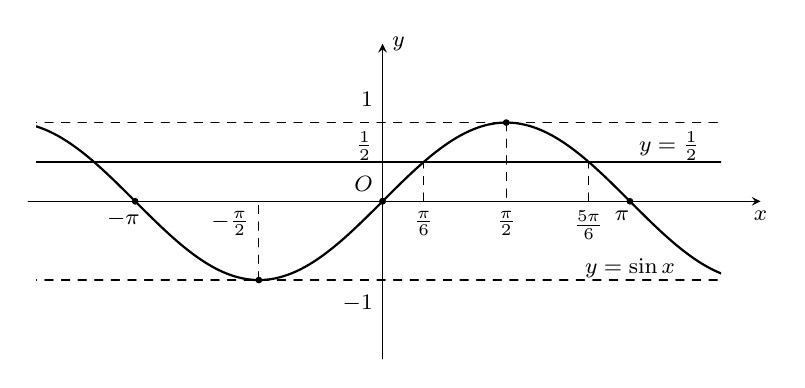
\begin{tikzpicture}[scale=1,>=stealth, font=\footnotesize, line join=round, line cap=round]
				\def\xmin{-4.5} \def\xmax{4.8} \def\ymin{-2} \def\ymax{2}
				\draw[->] (\xmin,0)--(\xmax,0) node [below]{$x$};
				\draw[->] (0,\ymin)--(0,\ymax) node [right]{$y$};
				\node at (0,0) [above left]{$O$};
				\clip (\xmin+0.1,\ymin+0.1) rectangle (\xmax-0.5,\ymax-0.1);
				\draw[smooth,samples=400,domain=\xmin:\xmax,thick] plot(\x,{sin(\x r)});
				\draw[smooth,samples=400,domain=\xmin:\xmax,thick] plot(\x,{1/2});
				\draw[dashed] (\xmin,1)--(\xmax,1) (\xmin,-1)--(\xmax,-1);
				\foreach \x in {-3*pi,-2.5*pi,-2*pi,-1.5*pi,-pi,-0.5*pi,0}
				{\draw[fill=black] (\x,sin \x*180/pi) circle (1pt);
					\draw[dashed] (\x,sin \x*180/pi)--(\x,0);
					\draw[fill=black] (-\x,sin -\x*180/pi) circle (1pt);
					\draw[dashed] (-\x,sin -\x*180/pi)--(-\x,0);}
				\node at (0,1.3) [left]{$1$};
				\node at (0,0.4) [above left]{$\frac{1}{2}$};
				\node at (0,-1.3) [left]{$-1$};
				\node at (-pi-0.15,0) [below]{$-\pi$};
				\node at (-0.5*pi,0) [below left]{$-\frac{\pi}{2}$};
				\node at (0.5*pi,0) [below]{$\frac{\pi}{2}$};
				\node at (1/6*pi,0) [below]{$\frac{\pi}{6}$};
				\node at (5/6*pi,0) [below]{$\frac{5\pi}{6}$};
				\node at (pi-0.1,0) [below]{$\pi$};
				\node at (pi,-1.1) [above]{$y=\sin x$};
				\node at (pi+0.5,0.4) [above]{$y=\frac{1}{2}$};
				\draw[dashed] (1/6*pi,0)--(1/6*pi,1/2) (5/6*pi,0)--(5/6*pi,1/2);
			\end{tikzpicture}
		\end{center}
		Quan sát hình vẽ ta thấy trên $[-\pi;\pi]$ đồ thị hàm số $y=\sin x$ cắt đường thẳng $y=\dfrac{1}{2}$ tại hai điểm $x=\dfrac{\pi}{6}$ và $x=\dfrac{5\pi}{6}$.\\
		Vậy các giá trị cần tìm là $x\in\left\{\dfrac{\pi}{6};\dfrac{5\pi}{6}\right\}$.	
	}
\end{bt}

\begin{bt}%[1D1H4-8]
% nguon: Archive/2024/TOAN_11_XE/TOAN_11_XE/data4/11C1/KNTT-1.3.tex #1179
%[Thành Đức Trung]
	Trong hình vẽ bên dưới, một chiếc máy bay $A$ bay ở độ cao $500$ m theo một đường thẳng đi ngang qua phía trên trạm quan sát $T$ ở mặt đất. Hình chiếu vuông góc của $A$ lên mặt đất là $H$, $\alpha$ là góc lượng giác $\left(Tx,TA\right)$ $\left(0<\alpha<\pi\right)$.
	\begin{center}
		\begin{tikzpicture}[>=stealth,x=1.0cm,y=1.0cm, scale=1]
			\draw[->](0,0) -- (14,0) node[below]{\footnotesize $x$ (m)};
			\draw[dashed,red](0,3) -- (14,3);
			\path
			(5,0) coordinate (T)
			(10,0) coordinate (H)
			(10,3) coordinate (A)
			;
			\draw[fill = black] (T) node [below]{\footnotesize$T$ (trạm quan sát)} circle (1pt) -- (H) node [below] {\footnotesize$H$} circle (1pt) -- (A) node [above]{\footnotesize$A$ (máy bay)} circle (1pt) -- (T);
			\draw (10,1.5) node [right]{\footnotesize $500$m};
			\draw pic[->,draw, angle radius=5mm]{angle=H--T--A} (T) node[shift={(10:.8)}]{$\alpha$};
			\path pic[draw,angle radius=6]{right angle=A--H--T};
		\end{tikzpicture}
	\end{center}
	\begin{enumerate}
		\item Biểu diễn tọa độ $x_H$ của điểm $H$ trên trục $Tx$ theo $\alpha$.
		\item Dựa vào đồ thị hàm số côtang, hãy cho biết với $\dfrac{\pi}{6} < \alpha < \dfrac{2\pi}{3}$ thì $x_H$ nằm trong khoảng nào? Làm tròn kết quả đến hàng phần mười.
	\end{enumerate}
	\loigiai{
		\begin{enumerate}
			\item Coi trạm quan sát $T$ là gốc tọa độ thì ta có
			\[x_H = \overline{TH} = AH\cdot\cot\alpha = 500\cot\alpha\;\left(\text{m}\right).\]
			\item \immini{
				Dựa vào đồ thị hàm số $\cot x$, ta thấy với $\dfrac{\pi}{6} < \alpha < \dfrac{2\pi}{3}$ thì $-\dfrac{\sqrt{3}}{3} < \cot \alpha < \sqrt{3}$.\\
				Do đó $-\dfrac{500\sqrt{3}}{3} < x_H < 500\sqrt{3}$. Làm tròn kết quả đến hàng phần mười ta được
				\[-288{,}7 < x_H< 866.\]
			}{
				\begin{tikzpicture}[font=\footnotesize,line join = round, line cap = round,>=stealth,scale=1]
					\draw[->] (-1,0) -- (4,0.)node[below]{\footnotesize $x$};
					\draw[->] (0,-3.1) -- (0,4.25)node[left]{\footnotesize $y$};
					\draw (0,0) node[above left] {\footnotesize $O$};
					\draw[dashed,smooth,samples=100,domain=0.25:2.8] plot(\x,{cot(((\x))*180/pi)});
					\draw[line width=1pt,smooth,red,samples=100,domain=pi/6:2*pi/3] plot(\x,{cot(((\x))*180/pi)});
					\draw[dashed] (pi,-3.1) -- (pi,0) node[below right]{$\pi$} -- (pi,4.2);
					\draw[dashed] (pi/6,0) node[below]{$\tfrac{\pi}{6}$} circle (1pt) --(pi/6,1.73)--(0,1.73) node[left]{$\sqrt{3}$};
					\draw[dashed] (2*pi/3,0) node[above]{$\tfrac{2\pi}{3}$} circle (1pt) --(2*pi/3,-0.577)--(0,-0.577) node[left]{$-\tfrac{\sqrt{3}}{3}$};
				\end{tikzpicture}
			}
		\end{enumerate}
	}
\end{bt}

\begin{bt}%[1D1N1-3]
% nguon: Archive/2024/TOAN_11_XE/TOAN_11_XE/data4/11C1/KNTT-1.1.tex #1180
%[Lê Minh Thiện Anh, dự án 11SGK-KNTT-2022]
	\immini{Cho góc hình học $uOv$ có số đo $60^\circ$. Xác định số đo của góc lượng giác ($Ou$, $Ov$) và ($Ov$, $Ou$).}
	{\begin{tikzpicture}[scale=0.77, font=\footnotesize, line join=round, line cap=round, >=stealth]		
		\draw (0,0) -- (4,0)node[below] {$u$};
		\draw[red] (0,0) -- (60:4)node[below right] {$v$};
		\draw (0:.6) arc (0:60:.6);
		\draw[-stealth] (2.75,1) arc (0:60:1);
		\path (30:3.5) node[below=-2pt]{$+$};
		\path (30:1) node{$60^\circ$};
		\path (0:0) node[below left]{$O$};
	\end{tikzpicture}}
	\loigiai{
		Ta có:
		\begin{itemize}
		\item Các góc lượng giác tia đầu $Ou$, tia cuối $Ov$ có số đo là sđ$(Ou,Ov)=60^\circ+k360^\circ$ $(k\in\mathbb{Z})$.
		\item Các góc lượng giác tia đầu $Ov$, tia cuối $Ou$ có số đo là sđ$(Ov,Ou)=-60^\circ+k360^\circ$ $(k\in\mathbb{Z})$.
		\end{itemize}
}
\end{bt}

\begin{bt}%[1D1N1-3]
% nguon: Archive/2024/TOAN_11_XE/TOAN_11_XE/data4/11C1/KNTT-1.1.tex #1181
 %[Lê Minh Thiện Anh, dự án 11SGK-KNTT-2022]
	Cho một góc lượng giác $(Ox, Ou)$ có số đo $-270^{\circ}$ và một góc lượng giác $(Ox, Ov)$ có số đo $135^{\circ}$. Tính số đo của các góc lượng giác $(Ou, Ov)$.
\loigiai{
Số đo của các góc lượng giác tia đầu $Ou$, tia cuối $Ov$ là
$$
\begin{aligned}
\text{sđ}(Ou, Ov) & =\text{sđ}(Ox, Ov)-\text{sđ}(Ox, Ou)+k 360^{\circ} \\
& =135^{\circ}-\left(-270^{\circ}\right)+k 360^{\circ}=405^{\circ}+k 360^{\circ} \\
& =45^{\circ}+(k+1) 360^{\circ}=45^{\circ}+m 360^{\circ}(m=k+1, m \in \mathbb{Z}).
\end{aligned}
$$
Vậy các góc lượng giác $(Ou, Ov)$ có số đo là $45^{\circ}+m 360^{\circ}(m \in \mathbb{Z})$.
}
\end{bt}

\begin{bt}%[1D1N1-2]
% nguon: Archive/2024/TOAN_11_XE/TOAN_11_XE/data4/11C1/KNTT-1.1.tex #1182
%[Lê Minh Thiện Anh, dự án 11SGK-KNTT-2022]
	a) Đổi từ độ sang rađian các số đo sau: $45^{\circ} ; 150^{\circ}$.\\
	b) Đổi từ rađian sang độ các số đo sau: $\dfrac{\pi}{3} ; \dfrac{5 \pi}{4}$.
	\loigiai{
		a) Ta có
		$$ 45^{\circ}=45 \cdot \frac{\pi}{180}=\frac{\pi}{4}; 
		150^{\circ}=150 \cdot \frac{\pi}{180}=\frac{5 \pi}{6}.$$
		b) Ta có
		$$\frac{\pi}{3}=\frac{\pi}{3} \cdot\left(\frac{180}{\pi}\right)^\circ=60^{\circ};
		\frac{5 \pi}{4}=\frac{5 \pi}{4} \cdot\left(\frac{180}{\pi}\right)^{\circ}=225^{\circ}.$$
}
\end{bt}

\begin{bt}%[1D1N1-5]
% nguon: Archive/2024/TOAN_11_XE/TOAN_11_XE/data4/11C1/KNTT-1.1.tex #1184
%[Lê Minh Thiện Anh, dự án 11SGK-KNTT-2022]
	Xác định các điểm $M$ và $N$ trên đường tròn lượng giác lần lượt biểu diễn các góc lượng giác có số đo bằng $\dfrac{13 \pi}{4}$ và $-150^{\circ}$.
	\loigiai{
	\immini{Điểm $M$ trên đường đường tròn lượng giác biểu diễn góc lượng giác có số đo bằng $\dfrac{13 \pi}{4}$ được xác định trong hình bên.\\
	Điểm $N$ trên đường tròn lượng giác biểu diễn góc lượng giác có số đo bằng $-150^{\circ}$ được xác định trong hình bên.}
	{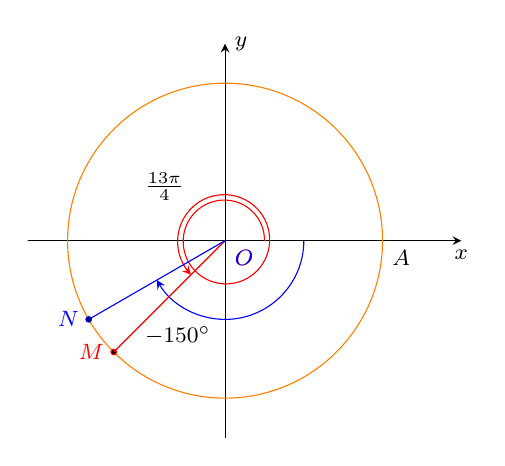
\begin{tikzpicture}[scale=1, font=\footnotesize, line join=round, line cap=round, >=stealth]		
		\draw[-stealth] (-2.5,0) -- (3,0)node[below] {$x$};
		\draw[-stealth] (0,-2.5) -- (0,2.5)node[right] {$y$};
		\draw[orange] (0,0) circle (2);
		\draw[red,-stealth,smooth,samples=100] plot[domain =0:3.25*pi]({.5*(1.02)^(\x) *cos(\x r)},{.5*(1.02)^(\x) *sin(\x r)});
		\draw[-stealth,blue] (0:1) arc (0:-150:1);
		\draw[red,fill=black] (0:0) node[below right]{$O$}--(585:2) circle(1pt) node[left]{$M$};
		\draw[blue,fill=black] (0:0) node[below right]{$O$}--(-150:2) circle(1pt) node[left]{$N$};
		\path (-120:1.2) node[below=-2pt]{$-150^{\circ}$};
		\path (130:1.2) node[below=-2pt]{$\frac{13\pi}{4}$};
		\path (0:2) node[below right]{$A$};
		\end{tikzpicture}}
	}
\end{bt}

\begin{bt}%[1D1N1-5]
% nguon: Archive/2024/TOAN_11_XE/TOAN_11_XE/data4/11C1/KNTT-1.1.tex #1185
%[Lê Minh Thiện Anh, dự án 11SGK-KNTT-2022]
Cho góc lượng giác có số đo bằng $-\dfrac{\pi}{3}$.
\begin{enumerate}
\item Xác định điểm $M$ trên đường tròn lượng giác biểu diễn góc lượng giác đã cho.
\item Tính các giá trị lượng giác của góc lượng giác đã cho.
\end{enumerate}
\loigiai{
\immini{\begin{enumerate}
\item Điểm $M$ trên đường tròn lượng giác biểu diễn góc lượng giác có số đo là $-\dfrac{\pi}{3}$ được xác định trong hình bên.
\item Ta có $\cos\left(-\dfrac{\pi}{3}\right)=\dfrac{1}{2}$; $\sin\left(-\dfrac{\pi}{3}\right)=-\dfrac{\sqrt{3}}{2}$;\\
$\tan\left(-\dfrac{\pi}{3}\right)=\dfrac{\sin\left(-\dfrac{\pi}{3}\right)}{\cos\left(-\dfrac{\pi}{3}\right)}=-\sqrt{3}$;\\ $\cot\left(-\dfrac{\pi}{3}\right)=\dfrac{\cos\left(-\dfrac{\pi}{3}\right)}{\sin\left(-\dfrac{\pi}{3}\right)}=-\dfrac{1}{\sqrt{3}}$.
\end{enumerate}}
{\begin{tikzpicture}[line join = round, line cap = round, >=stealth, font=\footnotesize, scale=0.6]
	\tikzset{label style/.style={font=\footnotesize}}
	\path (0,0) coordinate (O)
	(3,0) coordinate (A)
	(0,-3) coordinate (B)
	(0:0)++(-60:3) coordinate (M)
	($(O)!(M)!(A)$) coordinate (H)
	($(O)!(M)!(B)$) coordinate (K)
	;
	\draw[->] (-4,0) -- (4,0) node[above,blue]{$x$};
	\draw[->] (0,-4) -- (0.,4) node[left,blue]{$y$};
	\draw[orange] (O) circle (3cm);
	\draw[rotate=0,->,green!50!black] (0.5,0) arc (0:-60:0.6cm);
	\draw (0.85,-0.45) node[blue] {$-\frac{\pi}{3}$};
	\draw[dashed] (H)--(M)--(K);
	\draw[green!50!black] (M)--(O);
	\draw[blue] (1.5,0) node[above]{$\frac{1}{2}$}(0,-2.57) node[left]{$-\frac{\sqrt{3}}{2}$};
	\foreach \p/\r in {A/-45,M/-60,O/-150}
	\fill (\p) circle (1pt) node[shift={(\r:3mm)},blue]{$\p$};
	\end{tikzpicture}}
}
\end{bt}

\begin{bt}%[1D1H2-2]
% nguon: Archive/2024/TOAN_11_XE/TOAN_11_XE/data4/11C1/KNTT-1.1.tex #1186
%[Lê Minh Thiện Anh, dự án 11SGK-KNTT-2022]
Sử dụng máy tính cầm tay để tính $\sin \left(-\dfrac{9 \pi}{4}\right)$; tan $63^{\circ} 52' 41''$ (làm tròn kết quả đến chữ số thập phân thứ tư).
\loigiai{
\begin{center}
\renewcommand{\arraystretch}{2}
\begin{tabular}{|c|c|c|c|}
\hline 
Tính  & Bấm phím & Màn hình& Kết quả \\ 
\hline 
$\sin \left(-\dfrac{9 \pi}{4}\right)$ & \menuk\ \menuk\ \menuk\ \twok \openk  \signk \ninek  \shiftk \divk \fourk \closek \equalk & $-0.707106$ & $-0{,}7071$ \\ 
\hline 
$\tan 63^{\circ} 52'41''$ & \menuk\ \menuk\ \menuk\ \onek  \tank  \sixk \threek \circk  \fivek \twok  \circk \fourk \onek \circk \equalk & $2.03927$ & $2{,}0393$ \\ 
\hline 
\end{tabular} 
\end{center}
}
\end{bt}

\begin{bt}%[1D1H1-2]
% nguon: Archive/2024/TOAN_11_XE/TOAN_11_XE/data4/11C1/KNTT-1.1.tex #1187
%[Lê Minh Thiện Anh, dự án 11SGK-KNTT-2022]
\begin{enumerate}
\item Đổi $33^{\circ} 45'$ sang rađian;
\item Đổi $\dfrac{3}{4}$ (rad) sang độ.
\end{enumerate}
\loigiai{
\begin{center}
\renewcommand{\arraystretch}{2}
\begin{tabular}{|c|c|c|c|}
\hline 
Đổi số đo  & Bấm phím & Màn hình& Kết quả \\ 
\hline 
$33^{\circ} 45'$ & \menuk\ \menuk\ \menuk\ \twok \threek \threek \circk   \fourk \fivek \circk \shiftk \ansk \onek \equalk & $0.589048622$ & $0{,}5890$ (rad) \\ 
\hline 
$\dfrac{3}{4}$ (rad) & \menuk\ \menuk\ \menuk\ \onek \openk \threek  \divk   \fourk  \closek \shiftk \ansk \twok \equalk \circk & $42^{\circ} 58' 19''$ & $42^{\circ} 58' 19''$ \\ 
\hline 
\end{tabular} 
\end{center}
}
\end{bt}

\begin{bt}%[1D1N1-2]
% nguon: Archive/2024/TOAN_11_XE/TOAN_11_XE/data4/11C1/KNTT-1.1.tex #1188

	Đổi $50^\circ$ sang rađian.\dapso{$50^{\circ}=\dfrac{5\pi}{18}\,\mathrm{rad}$.}
	\loigiai{
		Ta có $1^{\circ}=\dfrac{\pi}{180}\,\mathrm{rad}$.\\
		Nên $50^{\circ}=\cdot\dfrac{\pi}{180}=\dfrac{5\pi}{18}\,\mathrm{rad}$.}
\end{bt}

\begin{bt}%[1D1N1-2]
% nguon: Archive/2024/TOAN_11_XE/TOAN_11_XE/data4/11C1/KNTT-1.1.tex #1189

	Đổi $\dfrac{3\pi}{4}\,\mathrm{rad}$ sang độ.\dapso{$\dfrac{3\pi}{4}\,\mathrm{rad}=135^\circ$.}
	\loigiai{
		Ta có $1\,\mathrm{rad}=\left(\dfrac{180}{\pi}\right)^\circ$.\\
		Nên $\dfrac{3\pi}{4}\,\mathrm{rad}=\left(\dfrac{3\pi}{4}\cdot\dfrac{180}{\pi}\right)^\circ=135^\circ$.}
\end{bt}

\begin{bt}%[1D1N1-2]
% nguon: Archive/2024/TOAN_11_XE/TOAN_11_XE/data4/11C1/KNTT-1.1.tex #1190

	\begin{enumerate}
		\item Đổi từ độ sang rađian các số đo sau: $45^{\circ} ; 150^{\circ}$.
		\item Đổi từ rađian sang độ các số đo sau: $\dfrac{\pi}{3} ; \dfrac{5 \pi}{4}$.
	\end{enumerate}
	\loigiai{
		\begin{enumerate}
			\item Ta có
			$$
			\begin{aligned}
				& 45^{\circ}=45 \cdot \frac{\pi}{180}=\frac{\pi}{4}, \\
				& 150^{\circ}=150 \cdot \frac{\pi}{180}=\frac{5 \pi}{6} .
			\end{aligned}
			$$
			\item Ta có
			$$
			\begin{aligned}
				& \frac{\pi}{3}=\frac{\pi}{3} \cdot\left(\frac{180}{\pi}\right)^\circ=60^{\circ}, \\
				& \frac{5 \pi}{4}=\frac{5 \pi}{4} \cdot\left(\frac{180}{\pi}\right)^{\circ}=225^{\circ} .
			\end{aligned}
			$$
		\end{enumerate}
	}
\end{bt}

\begin{bt}%[1D1H1-2]
% nguon: Archive/2024/TOAN_11_XE/TOAN_11_XE/data4/11C1/KNTT-1.1.tex #1191
%[DCHT Toán 11 - KNTT - Dương Quang]
	Đổi số đo của các góc sau ra rađian: $72^\circ; 600^\circ; -37^\circ45'30''$.
	\loigiai{
		Vì $1^\circ=\dfrac{\pi}{180}\, \mathrm{rad}$ nên\\
		$72^\circ=72\cdot\dfrac{\pi}{180}=\dfrac{2\pi}{5}$;\\
		$600^\circ=600\cdot\dfrac{\pi}{180}=\dfrac{10\pi}{3}$;\\
		$-37^\circ45'30''=-37^\circ-\left(\dfrac{45}{60}\right)^\circ-\left(\dfrac{30}{60 \cdot 60}\right) ^\circ=\left(\dfrac{4531}{120}\right)^\circ =\dfrac{4531}{120}\cdot\dfrac{\pi}{180}\approx 0,6587$.
	}
\end{bt}

\begin{bt}%[1D1H1-2]
% nguon: Archive/2024/TOAN_11_XE/TOAN_11_XE/data4/11C1/KNTT-1.1.tex #1192
%[DCHT Toán 11 - KNTT - Dương Quang]
	Đổi số đo của các góc sau ra độ: $\dfrac{5\pi}{18}; \dfrac{3\pi}{5}; -4$.
	\loigiai{
		Vì $1\, \mathrm{rad}=\left(\dfrac{180}{\pi}\right)^\circ$ nên\\
		$\dfrac{5\pi}{18}=\left(\dfrac{5\pi}{18}\cdot\dfrac{180}{\pi}\right)^\circ =50^\circ$;
		$\dfrac{3\pi}{5}=\left(\dfrac{3\pi}{5}\cdot \dfrac{180}{\pi}\right)^\circ =108^\circ$;
		$-4=-\left(4\cdot\dfrac{180}{\pi}\right)^\circ \approx -2260^\circ 48'$.
	}
\end{bt}

\begin{bt}%[1D1H1-2]
% nguon: Archive/2024/TOAN_11_XE/TOAN_11_XE/data4/11C1/KNTT-1.1.tex #1193
%[DCHT Toán 11 - KNTT - Dương Quang]
	Hoàn thành bảng chuyển đổi số đo độ và số đo rađian của một số góc đặc biệt sau
	\begin{center}
		\begin{longtable}{|c|c|c|c|c|c|c|c|}
			\hline
			Độ & $30^\circ$ & ? & $60^\circ$ & ? & $120^\circ$ & ? & $180^\circ$\\
			\hline
			Radian & ? & $\dfrac{\pi}{4}$ & ? & $\dfrac{\pi}{2}$ & ? & $\dfrac{3\pi}{4}$ & ? \\
			\hline
		\end{longtable}
	\end{center}
	\loigiai{
		Ta có bảng chuyển đổi số đo độ và số đo rađian của một số góc đặc biệt.
		\begin{center}
			\begin{longtable}{|c|c|c|c|c|c|c|c|}
				\hline
				Độ & $30^\circ$ & $45^\circ$ & $60^\circ$ & $90^\circ$ & $120^\circ$ & $135^\circ$ & $180^\circ$\\
				\hline
				Radian & $\dfrac{\pi}{6}$ & $\dfrac{\pi}{4}$ & $\dfrac{\pi}{3}$ & $\dfrac{\pi}{2}$ & $\dfrac{2\pi}{3}$ & $\dfrac{3\pi}{4}$ & $\pi$ \\
				\hline
			\end{longtable}
		\end{center}}
\end{bt}

\begin{bt}%[1D1N1-3]
% nguon: Archive/2024/TOAN_11_XE/TOAN_11_XE/data4/11C1/KNTT-1.1.tex #1194

	Xác định số đo của các góc lượng giác $(Oa,Ob)$ trong hình sau
	\begin{listEX}[4]
		\item 
		\begin{tikzpicture}[>=stealth,line join=round,line cap=round,font=\footnotesize,scale=0.8]
			\def\r{2.5}
			\path 
			(0,0) coordinate (O)
			(\r,0) coordinate (a)
			(0,\r) coordinate (b)
			;
			\pic[draw,angle radius=2mm,angle eccentricity=1.5] {right angle = a--O--b};
			\draw (a)--(O)--(b);
			\draw[->] (0:0.5*\r) arc (0:90:0.5*\r);
			\fill[black] (O) circle (1pt);
			\foreach \l/\g in {a/-90,b/180,O/-135}
			\draw[fill=black] (\l)+(\g:.3) node{$\l$};
		\end{tikzpicture}
		\item 
		\begin{tikzpicture}[>=stealth,line join=round,line cap=round,font=\footnotesize,scale=0.8]
			\def\r{2.5}
			\path 
			(0,0) coordinate (O)
			(\r,0) coordinate (a)
			(0,\r) coordinate (b)
			;
			\pic[draw,angle radius=2mm,angle eccentricity=1.5] {right angle = a--O--b};
			\draw (a)--(O)--(b);
			\draw[->,domain=0:450,variable=\t,samples=200,>=latex]
			plot ({0.6*(\t+2*450)*cos(\t)/(2*450)},
			{0.6*(\t+ 2*450)*sin(\t)/(2*450)})
			;
			\fill[black] (O) circle (1pt);
			\foreach \l/\g in {a/-90,b/180,O/-135}
			\draw[fill=black] (\l) +(\g:.3) node{$\l$};
		\end{tikzpicture}
		\item 
		\begin{tikzpicture}[>=stealth,line join=round,line cap=round,font=\footnotesize,scale=0.8]
			\def\r{2.5}
			\path 
			(0,0) coordinate (O)
			(\r,0) coordinate (a)
			(0,\r) coordinate (b)
			;
			\pic[draw,angle radius=2mm,angle eccentricity=1.5] {right angle = a--O--b};
			\draw (a)--(O)--(b);
			\draw[->,domain=0:810,variable=\t,samples=200,>=latex]
			plot ({0.6*(\t+2*810)*cos(\t)/(2*810)},
			{0.6*(\t+ 2*810)*sin(\t)/(2*810)})
			;
			\fill[black] (O) circle (1pt);
			\foreach \l/\g in {a/-90,b/180,O/-135}
			\draw[fill=black] (\l) +(\g:.3) node{$\l$};
		\end{tikzpicture}
		\item 
		\begin{tikzpicture}[>=stealth,line join=round,line cap=round,font=\footnotesize,scale=0.8]
			\def\r{2.5}
			\path 
			(0,0) coordinate (O)
			(\r,0) coordinate (a)
			(0,\r) coordinate (b)
			;
			\pic[draw,angle radius=2mm,angle eccentricity=1.5] {right angle = a--O--b};
			\draw (a)--(O)--(b);
			\draw[->] (0:0.3*\r) arc (0:-270:0.3*\r);
			\fill[black] (O) circle (1pt);
			\foreach \l/\g in {a/-90,b/180,O/-135}
			\draw[fill=black] (\l) +(\g:.3) node{$\l$};
		\end{tikzpicture}
	\end{listEX}
	\loigiai{
		\begin{listEX}[1]
			\item Số đo của góc lượng giác $(Oa,Ob)$ trong hình vẽ là $90^\circ$.
			\item Số đo của góc lượng giác $(Oa,Ob)$ trong hình vẽ là $90^\circ + 360^\circ = 450^\circ$.
			\item Số đo của góc lượng giác $(Oa,Ob)$ trong hình vẽ là $90^\circ + 2\cdot 360^\circ = 810^\circ$.
			\item Số đo của góc lượng giác $(Oa,Ob)$ trong hình vẽ là $\dfrac{3}{4}\cdot \left(-360^\circ\right)=-270^\circ$.
		\end{listEX}
	}
\end{bt}

\begin{bt}%[1D1N1-4]
% nguon: Archive/2024/TOAN_11_XE/TOAN_11_XE/data4/11C1/KNTT-1.1.tex #1195

	Một đường tròn có bán kính $20$ cm. Tìm độ dài các cung trên đường tròn đó có số đo sau:
	\begin{multicols}{4}
		\begin{enumerate}
			\item $\dfrac{\pi}{12}$;
			\item $1{,}5$;
			\item $35^\circ$;
			\item $315^\circ$.
		\end{enumerate}
	\end{multicols}
	\loigiai{
		\begin{enumerate}
			\item $l=R\alpha=20\cdot\dfrac{\pi}{12}=\dfrac{5\pi}{3}$ cm;
			\item $l=R\alpha=20\cdot1{,}5=30$ cm;
			\item Đổi $35^{\circ}=35 \cdot \dfrac{\pi}{180}=\dfrac{7\pi}{36} \mathrm{rad}$.\\
			Độ dài cung tròn là  $l=R\alpha=20\cdot\dfrac{7\pi}{36}=\dfrac{35\pi}{9}$ cm;
			\item Đổi $315^{\circ}=315 \cdot \dfrac{\pi}{180}=\dfrac{7\pi}{4} \mathrm{rad}$.\\
			Độ dài cung tròn là  $l=R\alpha=20\cdot\dfrac{7\pi}{4}=35$ cm.
		\end{enumerate}
	}
\end{bt}

\begin{bt}%[1D1H1-6]
% nguon: Archive/2024/TOAN_11_XE/TOAN_11_XE/data4/11C1/KNTT-1.1.tex #1196

	Một vệ tinh được định vị tại vị trí $A$ trong không gian. Từ vị trí $A$, vệ tinh bắt đầu chuyển động quanh Trái Đất theo quỹ đạo là đường tròn với tâm là tâm $O$ của Trái Đất, bán kính $9~000$ km. Biết rằng vệ tinh chuyển động hết một vòng của quỹ đạo trong $2$ giờ.
	\begin{enumerate}
		\item Hãy tính quãng đường vệ tinh đã chuyển động được sau $1$ giờ; $3$ giờ; $5$ giờ.
		\item Vệ tinh chuyển động được quãng đường $200~000$ km sau bao nhiêu giờ (làm tròn đến kết quả hàng đơn vị)?
	\end{enumerate}
	\loigiai{
		\begin{enumerate}
			\item Sau $1$ giờ, vệ tinh chuyển động hết $\dfrac{1}{2}$ vòng của quỹ đạo.\\
			Suy ra quãng đường vệ tinh đã chuyển động là $$S=\dfrac{1}{2}\cdot 2\pi\cdot  9~000=9~000\pi\approx 28247{,}3\text{ km.}$$
			Sau $3$ giờ, vệ tinh chuyển động hết $\dfrac{3}{2}$ vòng của quỹ đạo.\\
			Suy ra quãng đường vệ tinh đã chuyển động là $$S=\dfrac{3}{2}\cdot 2\pi \cdot 9~000=27~000\pi\approx 84823\text{ km.}$$
			Sau $5$ giờ, vệ tinh chuyển động hết $\dfrac{5}{2}$ vòng của quỹ đạo.\\
			Suy ra quãng đường vệ tinh đã chuyển động là $$S=\dfrac{5}{2}\cdot 2\pi\cdot 9~000=45~000\pi\approx 141371{,}7\text{ km.}$$
			\item Vệ tinh chuyển động được quãng đường $200~000$ km. Gọi $x$ là thời gian vệ tinh chuyển động. Khi đó
			$$200~000=x\cdot 2\pi \cdot 9~000\Leftrightarrow x\approx 11{,}1\text{ giờ}.$$
		\end{enumerate}
	}
\end{bt}

\begin{bt}%[1D1V1-5]
% nguon: Archive/2024/TOAN_11_XE/TOAN_11_XE/data4/11C1/KNTT-1.1.tex #1197
 
	Biểu diễn trên đường tròn lượng giác các góc lượng giác có số đo sau (với $k$ là số nguyên tùy ý)
	\begin{enumEX}{2}
		\item $\alpha=k\pi$;
		\item $\alpha=\dfrac{\pi}{3}+k\pi$.
	\end{enumEX}
	\loigiai{\immini{
			\begin{enumerate}
				\item Ta có $\alpha=k\pi=\dfrac{k2\pi}{2}$ do đó có hai điểm biểu diễn bởi góc có số đo $\alpha$.\\
				Với $k=0$, ta có $\alpha=0$ được biểu diễn bởi điểm $A_1$.\\
				Với $k=1$, ta có $\alpha=\pi$ được biểu diễn bởi điểm $A_2$.
				\item Ta có $\alpha=\dfrac{\pi}{3}+k\pi=\dfrac{\pi}{3}+\dfrac{k2\pi}{2}$ do đó có hai điểm biểu diễn bởi góc có số đo $\alpha$.\\
				Với $k=0$, ta có $\alpha=\dfrac{\pi}{3}$ được biểu diễn bởi điểm $B_1$.\\
				Với $k=1$, ta có $\alpha=\dfrac{4\pi}{3}$ được biểu diễn bởi điểm $B_2$.
			\end{enumerate}
		}{
			\begin{tikzpicture}[scale=.7,>=stealth, font=\footnotesize, line join=round, line cap=round]
				\draw[fill=black](0,0) coordinate (O) node[below left]{$O$} circle (1.5pt) (2,0) coordinate (A) node[above right] {$A_1$} circle (1.5pt) (180:2) coordinate (A2) node [above left] {$A_2$} circle (1.5 pt) (60:2) coordinate (B1) node [above right] {$B_1$} circle (1.5pt) (240:2) coordinate (B2) node [below left] {$B_2$} circle (1.5pt);
				\draw[very thick] (0,0) circle (2 cm);
				\draw[->] (-3,0)--(3,0) node [below]{$x$};
				\draw[->] (0,-3)--(0,3) node [left]{$y$};
				\clip (-5,-5) rectangle (5,5);
			\end{tikzpicture}
		}
	}
\end{bt}

\begin{bt}%[1D1H1-5]
% nguon: Archive/2024/TOAN_11_XE/TOAN_11_XE/data4/11C1/KNTT-1.1.tex #1198
 
	Biểu diễn trên đường tròn lượng giác các góc lượng giác có số đo là 
	\begin{enumEX}{4}
		\item $865^{\circ}$;
		\item $-1485^{\circ}$;
		\item $\dfrac{13}{3}\pi$;
		\item $-\dfrac{7}{3}\pi$.
	\end{enumEX}
	\loigiai{
		\begin{enumerate}
			\item Ta có $865^{\circ}=145^{\circ}+2\cdot360^{\circ}$. Vậy điểm biểu diễn góc lượng giác có số đo $865^{\circ}$ là điểm $M$ trên phần đường tròn lượng giác thuộc góc phần tư thứ II sao cho $\widehat{A O M}=145^{\circ}$. 
			\begin{center}
				\begin{tikzpicture}[scale=.8,>=stealth, font=\footnotesize, line join=round, line cap=round]
					\draw[fill=black](0,0) coordinate (O) node[below left]{$O$} circle (1.5pt) (2,0) coordinate (A) node[above right] {$A$} circle (1.5pt) (145:2) coordinate (M) node [left] {$M$} circle (1.5 pt);
					\draw[very thick] (0,0) circle (2 cm);
					\draw[->] (-3,0)--(3,0) node [below]{$x$};
					\draw[->] (0,-3)--(0,3) node [left]{$y$};
					\clip (-3,-3) rectangle (3,3);
					\draw (2.5,2.5) node {I} (-2.5,2.5) node {II} (-2.5,-2.5) node {III} (2.5,-2.5) node {IV};
					\draw (M)--(O);
					\pic [draw, ->, "$\alpha$", angle eccentricity=1.5] {angle = A--O--M};
				\end{tikzpicture}
			\end{center}
			\item Ta có $-1485^{\circ}=-45^{\circ}-3\cdot360^{\circ}$. Vậy điểm biểu diễn góc lượng giác có số đo $-1485^{\circ}$ là điểm $M$ trên phần đường tròn lượng giác thuộc góc phần tư thứ IV sao cho  $\widehat{A O M}=145^{\circ}$.
			\begin{center}
				\begin{tikzpicture}[scale=.8,>=stealth, font=\footnotesize, line join=round, line cap=round]
					\draw[fill=black](0,0) coordinate (O) node[below left]{$O$} circle (1.5pt) (2,0) coordinate (A) node[above right] {$A$} circle (1.5pt) (-45:2) coordinate (M) node [below right] {$M$} circle (1.5 pt);
					\draw[very thick] (0,0) circle (2 cm);
					\draw[->] (-3,0)--(3,0) node [below]{$x$};
					\draw[->] (0,-3)--(0,3) node [left]{$y$};
					\clip (-3,-3) rectangle (3,3);
					\draw (2.5,2.5) node {I} (-2.5,2.5) node {II} (-2.5,-2.5) node {III} (2.5,-2.5) node {IV};
					\draw (M)--(O);
					\pic [draw, <-, "$\alpha$", angle eccentricity=1.5] {angle = M--O--A};
				\end{tikzpicture}
			\end{center}
			\item Ta có $\dfrac{13}{3}\pi=\dfrac{\pi}{3}+2\cdot2\pi$. Vậy điểm biểu diễn góc lượng giác có số đo $\dfrac{13}{3}\pi$ là điểm $M$ trên phần đường tròn lượng giác thuộc góc phần tư thứ I sao cho $\widehat{A O M}=\dfrac{\pi}{3}$. 
			\begin{center}
				\begin{tikzpicture}[scale=.8,>=stealth, font=\footnotesize, line join=round, line cap=round]
					\draw[fill=black](0,0) coordinate (O) node[below left]{$O$} circle (1.5pt) (2,0) coordinate (A) node[above right] {$A$} circle (1.5pt) (60:2) coordinate (M) node [above right] {$M$} circle (1.5 pt);
					\draw[very thick] (0,0) circle (2 cm);
					\draw[->] (-3,0)--(3,0) node [below]{$x$};
					\draw[->] (0,-3)--(0,3) node [left]{$y$};
					\clip (-3,-3) rectangle (3,3);
					\draw (2.5,2.5) node {I} (-2.5,2.5) node {II} (-2.5,-2.5) node {III} (2.5,-2.5) node {IV};
					\draw (M)--(O);
					\pic [draw, ->, "$\alpha$", angle eccentricity=1.5] {angle = A--O--M};
				\end{tikzpicture}
			\end{center}
			\item Ta có $-\dfrac{7}{3}\pi=-\dfrac{\pi}{3}-2\pi$. Vậy điểm biểu diễn góc lượng giác có số đo $-\dfrac{7}{3}\pi$ là điểm $M$ trên phần đường tròn lượng giác thuộc góc phần tư thứ IV sao cho $\widehat{A O M}=\dfrac{\pi}{3}$. 
			\begin{center}
				\begin{tikzpicture}[scale=.8,>=stealth, font=\footnotesize, line join=round, line cap=round]
					\draw[fill=black](0,0) coordinate (O) node[below left]{$O$} circle (1.5pt) (2,0) coordinate (A) node[above right] {$A$} circle (1.5pt) (-60:2) coordinate (M) node [below right] {$M$} circle (1.5 pt);
					\draw[very thick] (0,0) circle (2 cm);
					\draw[->] (-3,0)--(3,0) node [below]{$x$};
					\draw[->] (0,-3)--(0,3) node [left]{$y$};
					\clip (-3,-3) rectangle (3,3);
					\draw (2.5,2.5) node {I} (-2.5,2.5) node {II} (-2.5,-2.5) node {III} (2.5,-2.5) node {IV};
					\draw (M)--(O);
					\pic [draw, <-, "$\alpha$", angle eccentricity=1.5] {angle = M--O--A};
				\end{tikzpicture}
			\end{center}
		\end{enumerate}
	}
\end{bt}

\begin{bt}%[1D1H2-2]
% nguon: Archive/2024/TOAN_11_XE/TOAN_11_XE/data4/11C1/KNTT-1.1.tex #1199

	Xét dấu các giá trị lượng giác của góc lượng giác $\alpha=-\dfrac{3 \pi}{4}$.
	\loigiai{
		Do $-\pi<-\dfrac{3 \pi}{4}<-\dfrac{\pi}{2}$ nên $\sin \left(-\dfrac{3 \pi}{4}\right)<0; \cos \left(-\dfrac{3 \pi}{4}\right)<0; \tan \left(-\dfrac{3 \pi}{4}\right)>0; \cot \left(-\dfrac{3 \pi}{4}\right)>0$.
	}
\end{bt}

\begin{bt}%[1D1V2-2]
% nguon: Archive/2024/TOAN_11_XE/TOAN_11_XE/data4/11C1/KNTT-1.1.tex #1200

	Xác định dấu các biểu thức:
	\begin{enumEX}{2}
		\item $A=\sin 50^{\circ} \cdot \cos \left(-100^{\circ}\right)$;
		\item $B=\sin 195^{\circ} \cdot \tan \dfrac{20 \pi}{7}$.
	\end{enumEX}
	\loigiai{
		\begin{enumerate}
			\item $A=\sin 50^{\circ} \cdot \cos \left(-100^{\circ}\right)$.\\
			Ta có điểm cuối của cung $50^{\circ}$ thuộc góc phần tư thứ I nên $\sin 50^{\circ}>0$. Điểm cuối của cung $-100^{\circ}$ thuộc góc phần tư thứ III nên $\cos \left(-100^{\circ}\right)<0$.\\
			Do đó, $A<0$.
			\item $B=\sin 195^{\circ} \cdot \tan \dfrac{20 \pi}{7}$.\\
			Ta có: điểm cuối của cung $195^{\circ}$ thuộc góc phần tư thứ III nên sin $195^{\circ}<0$. Điểm cuối của cung $\dfrac{20 \pi}{7}=\dfrac{6 \pi}{7}+2 \pi$ thuộc góc phần tư thứ II nên $\tan\dfrac{20 \pi}{7}<0$.\\ Do đó, $B>0$.
		\end{enumerate}
		
	}
\end{bt}

\begin{bt}%[1D1V2-2]
% nguon: Archive/2024/TOAN_11_XE/TOAN_11_XE/data4/11C1/KNTT-1.1.tex #1201

	Cho $\pi<\alpha<\dfrac{3 \pi}{2}$. Xét dấu các biểu thức sau:
	\begin{enumEX}{2}
		\item $A=\cos \left(\alpha-\dfrac{\pi}{2}\right)$;
		\item $B=\tan \left(\dfrac{2019 \pi}{2}-\alpha\right)$.
	\end{enumEX}
	\loigiai{
		\begin{enumerate}
			\item $A=\cos \left(\alpha-\dfrac{\pi}{2}\right)=\cos \left(\dfrac{\pi}{2}-\alpha\right)=\sin \alpha<0$.
			\item $B=\tan \left(\dfrac{2019 \pi}{2}-\alpha\right)=\tan \left(\dfrac{\pi}{2}-\alpha+1009 \pi\right)=\tan \left(\dfrac{\pi}{2}-\alpha\right)=\cot \alpha>0$.
		\end{enumerate}
	}
\end{bt}

\begin{bt}%[1D1H2-2]
% nguon: Archive/2024/TOAN_11_XE/TOAN_11_XE/data4/11C1/KNTT-1.1.tex #1203
%[DCHT Toán 11 - KNTT - Nguyễn Hoài Nam]
	Tính các giá trị lượng giác của góc $\alpha$, biết
	\begin{enumEX}{2}
		\item $\cos\alpha=\dfrac{1}{5}$ và $0<\alpha<\dfrac{\pi}{2}$;
		\item $\sin\alpha=\dfrac{2}{5}$ và $\dfrac{\pi}{2}<\alpha<\pi$;
		\item $\tan\alpha=\sqrt{5}$ và $\pi<\alpha<\dfrac{3\pi}{2}$;
		\item $\cot\alpha=-\dfrac{1}{\sqrt{2}}$ và $\dfrac{3\pi}{2}<\alpha<2\pi$.
	\end{enumEX}
	\loigiai{
		\begin{enumerate}[a)]
			\item Ta có $\sin^2\alpha+\cos^2\alpha=1\Rightarrow \sin^2\alpha=1-\cos^2\alpha\Leftrightarrow \hoac{& \sin\alpha=\sqrt{1-\cos^2\alpha}\\&\sin\alpha=-\sqrt{1-\cos^2\alpha}.}$\\
			Vì $0<\alpha<\dfrac{\pi}{2}$ nên $\sin\alpha>0$, suy ra $\sin\alpha=\sqrt{1-\cos^2\alpha}$.\\
			$\Rightarrow\sin\alpha=\sqrt{1-\left(\dfrac{1}{5}\right)^2}=\sqrt{\dfrac{24}{25}}=\dfrac{2\sqrt{6}}{5}$.\\
			Mà $\tan\alpha=\dfrac{\sin\alpha}{\cos\alpha}$ nên $\tan\alpha=\dfrac{2\sqrt{6}}{5}:\dfrac{1}{5}=2\sqrt{6}$ và $\cot\alpha=\dfrac{\sqrt{6}}{12}$.
			\item Ta có $\sin^2\alpha+\cos^2\alpha=1\Rightarrow \cos^2\alpha=1-\sin^2\alpha\Leftrightarrow \hoac{& \cos\alpha=\sqrt{1-\sin^2\alpha}\\&\cos\alpha=-\sqrt{1-\sin^2\alpha}.}$\\
			Vì $\dfrac{\pi}{2}<\alpha<\pi$ nên $\cos\alpha<0$, suy ra $\cos\alpha=-\sqrt{1-\sin^2\alpha}$.\\
			$\Rightarrow\cos\alpha=-\sqrt{1-\left(\dfrac{2}{5}\right)^2}=-\sqrt{\dfrac{21}{25}}=-\dfrac{\sqrt{21}}{5}$.\\
			Mà $\tan\alpha=\dfrac{\sin\alpha}{\cos\alpha}$ nên $\tan\alpha=\dfrac{2}{5}:\left(-\dfrac{\sqrt{21}}{5}\right)=-\dfrac{2\sqrt{21}}{21}$ và $\cot\alpha=-\dfrac{\sqrt{21}}{2}$.
			\item Vì $\pi<\alpha<\dfrac{3\pi}{2}$ nên $\cos\alpha<0$, do đó từ công thức:\\
			$1+\tan^2\alpha=\dfrac{1}{\cos^2\alpha}$, suy ra $\cos^2\alpha=\dfrac{1}{1+\tan^2\alpha}$.\\
			$\Rightarrow\cos\alpha=-\dfrac{1}{\sqrt{1+\tan^2\alpha}}=-\dfrac{1}{\sqrt{1+(\sqrt{5})^2}}=-\dfrac{\sqrt{6}}{6}$;\\ $\cot\alpha=\dfrac{1}{\tan\alpha}=\dfrac{\sqrt{5}}{5}$ và $\sin\alpha=\tan\alpha\cdot\cos\alpha=-\dfrac{\sqrt{30}}{6}$.
			\item 
			Vì $\dfrac{3\pi}{2}<\alpha<2\pi$ nên $\sin\alpha<0$, do đó từ công thức:\\
			$1+\cot^2\alpha=\dfrac{1}{\sin^2\alpha}$, suy ra $\sin^2\alpha=\dfrac{1}{1+\cot^2\alpha}$.\\
			$\Rightarrow\sin\alpha=-\dfrac{1}{\sqrt{1+\cot^2\alpha}}=-\dfrac{1}{\sqrt{1+\left(-\dfrac{1}{\sqrt{2}}\right)^2}}=-\dfrac{\sqrt{6}}{3}$;\\ $\tan\alpha=\dfrac{1}{\cot\alpha}=-\sqrt{2}$ và $\cos\alpha=\cot\alpha\cdot\sin\alpha=\dfrac{\sqrt{3}}{3}$.
		\end{enumerate}
	}
\end{bt}

\begin{bt}%[1D1H2-4]
% nguon: Archive/2024/TOAN_11_XE/TOAN_11_XE/data4/11C1/KNTT-1.1.tex #1204
%[DCHT Toán 11 - KNTT - Nguyễn Hoài Nam]
	Không dùng máy tính cầm tay, tính giá trị của biểu thức
	\[A=\cos \dfrac{\pi}{9}-\sin \dfrac{13\pi}{36}+\cos \dfrac{5\pi}{36}+\cos \dfrac{8\pi}{9}-\cos \pi.\]
	\loigiai{
		Ta có
		\begin{eqnarray*}
			A&=& \cos \dfrac{\pi}{9}-\sin \dfrac{13\pi}{36}+\cos \dfrac{5\pi}{36}+\cos \dfrac{8\pi}{9}-\cos \pi\\
			&=& \cos \dfrac{\pi}{9}-\sin \dfrac{13\pi}{36}+\sin \left(\dfrac{\pi}{2}-\dfrac{5\pi}{36}\right)+\cos \left(\pi-\dfrac{\pi}{9}\right)+1\\
			&=& \cos \dfrac{\pi}{9}-\sin \dfrac{13\pi}{36}+\sin \dfrac{13\pi}{36}-\cos \dfrac{\pi}{9}+1\\
			&=&1.
		\end{eqnarray*}
		Vậy $A=1$.
	}
\end{bt}

\begin{bt}%[1D1H2-4]
% nguon: Archive/2024/TOAN_11_XE/TOAN_11_XE/data4/11C1/KNTT-1.1.tex #1205
%[DCHT Toán 11 - KNTT - Nguyễn Hoài Nam]
	Tính giá trị đúng của các biểu thức sau (không dùng máy tính cầm tay).
	\begin{enumEX}{2}
		\item $A=\sin \dfrac{\pi}{36} + \sin \dfrac{5\pi}{6} - \sin \dfrac{35\pi}{36} + \sin \pi$;
		\item $B=\cos \dfrac{\pi}{12} + \cos \dfrac{7\pi}{36} - \sin \dfrac{5\pi}{12} - \sin \dfrac{11\pi}{36}$;
		\item $C=\tan \dfrac{5\pi}{36}\cdot \tan \dfrac{\pi}{4}\cdot \tan \dfrac{23\pi}{36}$;
		\item $D=\cot \dfrac{\pi}{18}\cdot \cot \dfrac{\pi}{6} \cdot \cot \dfrac{5\pi}{9}$.
	\end{enumEX}
	\loigiai
	{
		\begin{enumerate}[a)]
			\item $\begin{aligned}[t]
				A &=\sin \dfrac{\pi}{36} + \sin \dfrac{5\pi}{6} - \sin \dfrac{35\pi}{36} + \sin \pi = \sin \dfrac{\pi}{36} + \sin\left(\pi-\dfrac{\pi}{6}\right) - \sin\left(\pi-\dfrac{\pi}{36}\right) + \sin \pi\\
				&=\sin \dfrac{\pi}{36} + \sin \dfrac{\pi}{6} - \sin \dfrac{\pi}{36} + \sin \pi = \sin \dfrac{\pi}{6} + \sin \pi = \dfrac{1}{2}+0 = \dfrac{1}{2}.
			\end{aligned}$
			\item $\begin{aligned}[t]
				B &=\cos \dfrac{\pi}{12} + \cos \dfrac{7\pi}{36} - \sin \dfrac{5\pi}{12} - \sin \dfrac{11\pi}{36} = \cos \dfrac{\pi}{12} + \cos \dfrac{7\pi}{36} - \sin\left(\dfrac{\pi}{2}-\dfrac{\pi}{12}\right) - \sin\left(\dfrac{\pi}{2}-\dfrac{7\pi}{36}\right)\\
				&=\cos \dfrac{\pi}{12} + \cos \dfrac{7\pi}{36} - \cos \dfrac{\pi}{12} - \cos \dfrac{7\pi}{36} = 0.
			\end{aligned}$
			\item $\begin{aligned}[t]
				C &=\tan \dfrac{5\pi}{36}\cdot \tan \dfrac{\pi}{4}\cdot \tan \dfrac{23\pi}{36} = \tan \dfrac{5\pi}{36}\cdot \tan \dfrac{\pi}{4}\cdot \tan\left(\pi - \dfrac{13\pi}{36}\right)\\
				&= \tan \dfrac{5\pi}{36}\cdot \tan \dfrac{\pi}{4}\cdot \left(-\tan \dfrac{13\pi}{36}\right)=-\tan \dfrac{5\pi}{36}\cdot \tan \dfrac{\pi}{4}\cdot  \tan \dfrac{13\pi}{36} \\
				&=-\tan \dfrac{5\pi}{36}\cdot \tan \dfrac{\pi}{4}\cdot \tan\left(\dfrac{\pi}{2} - \dfrac{5\pi}{36}\right) = -\tan \dfrac{5\pi}{36}\cdot \tan \dfrac{\pi}{4}\cdot \cot \dfrac{5\pi}{36}\\
				&=-\left(\tan \dfrac{5\pi}{36} \cdot \cot \dfrac{5\pi}{36}\right)\tan \dfrac{\pi}{4} = -1\cdot 1 = -1.
			\end{aligned}$
			\item $\begin{aligned}[t]
				D &=\cot \dfrac{\pi}{18}\cdot \cot \dfrac{\pi}{6} \cdot \cot \dfrac{5\pi}{9} = \cot \dfrac{\pi}{18}\cdot \cot \dfrac{\pi}{6} \cdot \cot \left(\pi - \dfrac{4\pi}{9}\right)\\
				&=\cot \dfrac{\pi}{18}\cdot \cot \dfrac{\pi}{6} \cdot \left(-\cot \dfrac{4\pi}{9}\right) = -\cot \dfrac{\pi}{18}\cdot \cot \dfrac{\pi}{6}\cdot \cot \dfrac{4\pi}{9}\\
				&=-\cot \dfrac{\pi}{18}\cdot \cot \dfrac{\pi}{6}\cdot \cot\left(\dfrac{\pi}{2} - \dfrac{\pi}{18}\right) = -\cot \dfrac{\pi}{18}\cdot \cot \dfrac{\pi}{6} \cdot \tan \dfrac{\pi}{18}\\
				&=-\left(\cot \dfrac{\pi}{18} \cdot \tan \dfrac{\pi}{18}\right) \cot \dfrac{\pi}{6} = -1\cdot \sqrt{3} = -\sqrt{3}.
			\end{aligned}$
		\end{enumerate}
	}
\end{bt}

\begin{bt}%[1D1N1-2]
% nguon: Archive/2024/TOAN_11_XE/TOAN_11_XE/data4/11C1/KNTT-1.1.tex #1206

	\begin{multicols}{2}
	\begin{enumerate}
		\item Đổi $60^\circ$ sang rađian.\dapso{$60^{\circ}=\dfrac{\pi}{3}\,\mathrm{rad}$.}
		\item Đổi $\dfrac{2\pi}{3}\,\mathrm{rad}$ sang độ.\dapso{$\dfrac{2\pi}{3}\,\mathrm{rad}=120^\circ$.}
		\end{enumerate}
	\end{multicols}		
	\loigiai{
		\begin{enumerate}
			\item Ta có $1^{\circ}=\dfrac{\pi}{180}\,\mathrm{rad}$. Do đó  $60^{\circ}=60\cdot\dfrac{\pi}{180}=\dfrac{\pi}{3}\,\mathrm{rad}$.
			\item Ta có $1\,\mathrm{rad}=\left(\dfrac{180}{\pi}\right)^\circ$. Do đó 
			$\dfrac{2\pi}{3}\,\mathrm{rad}=\left(\dfrac{2\pi}{3}\cdot\dfrac{180}{\pi}\right)^\circ=120^\circ$.
		\end{enumerate}
		}
\end{bt}

\begin{bt}%[1D1N1-2]
% nguon: Archive/2024/TOAN_11_XE/TOAN_11_XE/data4/11C1/KNTT-1.1.tex #1207

	Hãy hoàn thành bảng chuyển đổi số đo độ và số đo rađian của một số góc sau.
	\begin{center}
		\begin{longtable}{|c|c|c|c|c|}
			\hline
			Độ & $18^\circ$ & ? & $72^\circ$ & ? \\
			\hline
			Radian & ? & $\dfrac{2\pi}{9}$ & ? & $\dfrac{5\pi}{6}$\\
			\hline
		\end{longtable}
	\end{center}
	\loigiai{
		Ta có bảng chuyển đổi số đo độ và số đo rađian của một số góc.
		\begin{center}
			\begin{longtable}{|c|c|c|c|c|}
				\hline
				Độ & $18^\circ$ & $40^\circ$ & $72^\circ$ & $150^\circ$ \\
				\hline
				Radian & $\dfrac{\pi}{10}$ & $\dfrac{2\pi}{9}$ & $\dfrac{2\pi}{5}$ & $\dfrac{5\pi}{6}$\\
				\hline
			\end{longtable}
		\end{center}
	}
\end{bt}

\begin{bt}%[1D1H1-2]
% nguon: Archive/2024/TOAN_11_XE/TOAN_11_XE/data4/11C1/KNTT-1.1.tex #1208

	Đổi các số đo góc sau đây từ rađian sang độ hoặc ngược lại
	\begin{listEX}[3]
		\item $-60^{\circ}$.
		\item $\dfrac{2 \pi}{5}\, \mathrm{rad}$.
		\item $3\, \mathrm{rad}$.
	\end{listEX}
	\loigiai{
		\begin{listEX}[2]
			\item $-60^{\circ}=-\dfrac{60 \pi}{180}\, \mathrm{rad}=-\dfrac{\pi}{3}\, \mathrm{rad}$.
			\item $\dfrac{2 \pi}{5}\, \mathrm{rad}=\left(\dfrac{2 \pi}{5}\cdot \dfrac{180}{\pi}\right)^{\circ}=72^{\circ}$.
			\item $3\, \mathrm{rad}=\left(3 \cdot \dfrac{180}{\pi}\right)^{\circ}=\left(\dfrac{540}{\pi}\right)^{\circ} \approx 171{,}89^{\circ}$.
		\end{listEX}	
	}
\end{bt}

\begin{bt}%[1D1H1-2]
% nguon: Archive/2024/TOAN_11_XE/TOAN_11_XE/data4/11C1/KNTT-1.1.tex #1209

	Đổi số đo của các góc sau ra rađian: $54^\circ; 30^\circ 45'; -60^\circ; -210^\circ$.
	\loigiai{
		\begin{itemize}
			\item $54^\circ=54\cdot\dfrac{\pi}{180}=\dfrac{3\pi}{10}$;
			\item $30^\circ 45'=30^\circ+\left(\dfrac{45}{60}\right)^\circ=\left(\dfrac{123}{4}\right)^\circ=\dfrac{123}{4}\cdot\dfrac{\pi}{180}=\dfrac{41\pi}{240}\approx 0,5367$;
			\item $-60^\circ=-60\cdot\dfrac{\pi}{180}=-\dfrac{\pi}{3}$;
			\item $-210^\circ=-210\cdot\dfrac{\pi}{180}=-\dfrac{7\pi}{6}$.
		\end{itemize}
	}
\end{bt}

\begin{bt}%[1D1H1-2]
% nguon: Archive/2024/TOAN_11_XE/TOAN_11_XE/data4/11C1/KNTT-1.1.tex #1210

	Đổi số đo của các góc sau ra độ: $\dfrac{\pi}{5}; -\dfrac{5\pi}{6}; \dfrac{4\pi}{3}; 3,56\pi$.
	\loigiai{\begin{multicols}{2}
		\begin{itemize}
			\item $\dfrac{\pi}{5}=\left(\dfrac{\pi}{5}\cdot\dfrac{180}{\pi}\right)^\circ=36^\circ$;
			\item $-\dfrac{5\pi}{6}=-\left(\dfrac{5\pi}{6}\cdot\dfrac{180}{\pi}\right)^\circ= 150^\circ$;
			\item $\dfrac{4\pi}{3}=\left(\dfrac{4\pi}{3}\cdot\dfrac{180}{\pi}\right)^\circ=240^\circ$;
			\item $3,56\pi=\left(3,56\pi\cdot\dfrac{180}{\pi}\right)^\circ\approx 640^\circ48'$.
		\end{itemize}
		\end{multicols}		
	}
\end{bt}

\begin{bt}%[1D1N1-2]
% nguon: Archive/2024/TOAN_11_XE/TOAN_11_XE/data4/11C1/KNTT-1.1.tex #1211
%[Lê Minh Thiện Anh, dự án 11SGK-KNTT-2022]
	Hoàn thành bảng sau
	\begin{center}
	\renewcommand{\arraystretch}{2}
	\begin{tabular}{|c|c|c|c|c|c|l|}
	\hline
	Số đo độ     & $15^\circ$ & ? & $0^\circ$ & $900^\circ$ & ? & ?  \\ \hline
	Số đo radian & ?  & $\dfrac{3\pi}{8}$ & ? & ?   & $-\dfrac{7\pi}{12}$ & $-\dfrac{11\pi}{8}$ \\ \hline
	\end{tabular}
	\end{center}
	\loigiai{
		\begin{center}
		\renewcommand{\arraystretch}{2}
		\begin{tabular}{|c|c|c|c|c|c|l|}
		\hline
		Số đo độ     & $15^\circ$ & $\left(\dfrac{135}{2}\right)^\circ$ & $0^\circ$ & $900^\circ$ & $-105^\circ$ & $-\left(\dfrac{495}{2}\right)^\circ$  \\ \hline
		Số đo radian & $\dfrac{\pi}{12}$  & $\dfrac{3\pi}{8}$ & $0$ & $5\pi$   & $-\dfrac{7\pi}{12}$ & $-\dfrac{11\pi}{8}$ \\ \hline
		\end{tabular}
		\end{center}
}
\end{bt}

\begin{bt}%[1D1N1-5]
% nguon: Archive/2024/TOAN_11_XE/TOAN_11_XE/data4/11C1/KNTT-1.1.tex #1212
%[Lê Minh Thiện Anh, dự án 11SGK-KNTT-2022]
	Trên đường tròn lượng giác, xác định điểm $M$ biểu diễn các góc lượng giác có số đo sau:
	\begin{multicols}{4}
	\begin{enumerate}
	\item $\dfrac{2\pi}{3}$;
	\item $-\dfrac{11\pi}{4}$;
	\item $150^\circ$;
	\item $-225^\circ$.
	\end{enumerate}
	\end{multicols}
	\loigiai{
	\begin{enumerate}
		\item Điểm $M$ trên đường đường tròn lượng giác biểu diễn góc lượng giác có số đo bằng $\dfrac{2\pi}{3}$ được xác định trong hình sau
		\begin{center}
		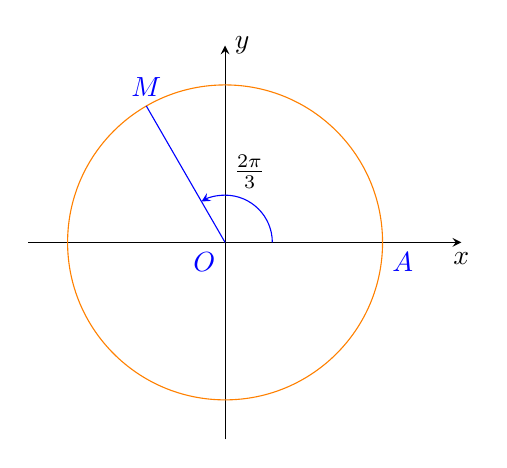
\begin{tikzpicture}		
			\draw[-stealth] (-2.5,0) -- (3,0)node[below] {$x$};
			\draw[-stealth] (0,-2.5) -- (0,2.5)node[right] {$y$};
			\draw[orange] (0,0) circle (2);
			\draw[-stealth,blue] (0:.6) arc (0:120:.6);
			\draw[blue] (0:0) node[below left]{$O$}--(120:2) node[above]{$M$};
			\path (75:1.2) node[below=-2pt]{$\frac{2\pi}{3}$};
			\path (0:2) node[below right,blue]{$A$};
			\end{tikzpicture}
			\end{center}
			\item Điểm $M$ trên đường đường tròn lượng giác biểu diễn góc lượng giác có số đo bằng $-\dfrac{11\pi}{4}$ được xác định trong hình sau
			\begin{center}
			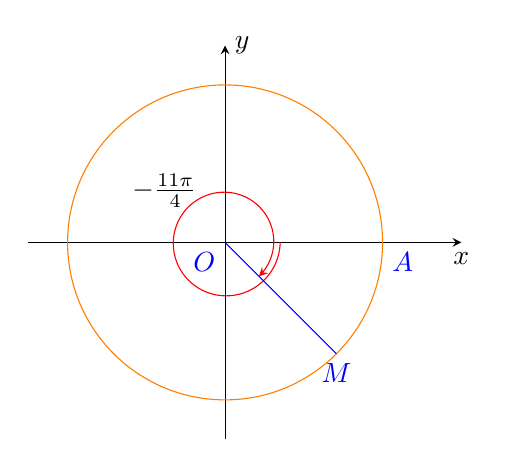
\begin{tikzpicture}		
				\draw[-stealth] (-2.5,0) -- (3,0)node[below] {$x$};
				\draw[-stealth] (0,-2.5) -- (0,2.5)node[right] {$y$};
				\draw[orange] (0,0) circle (2);
				\draw[red,-stealth,smooth,samples=100] plot[domain =0:-2.25*pi]({.7*(1.02)^(\x) *cos(\x r)},{.7*(1.02)^(\x) *sin(\x r)});
				\draw[blue] (0:0) node[below left]{$O$}--(-45:2) node[below]{$M$};
				\path (130:1.2) node[below=-2pt]{$-\frac{11\pi}{4}$};
				\path (0:2) node[below right,blue]{$A$};
				\end{tikzpicture}
			\end{center}
			\item Điểm $M$ trên đường đường tròn lượng giác biểu diễn góc lượng giác có số đo bằng $150^{\circ}$ được xác định trong hình sau
			\begin{center}
			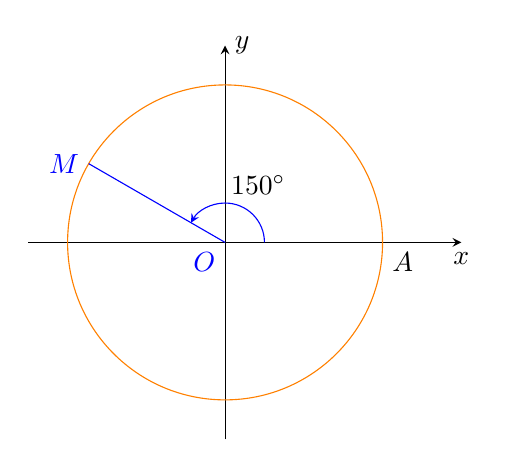
\begin{tikzpicture}		
				\draw[-stealth] (-2.5,0) -- (3,0)node[below] {$x$};
				\draw[-stealth] (0,-2.5) -- (0,2.5)node[right] {$y$};
				\draw[orange] (0,0) circle (2);
				\draw[-stealth,blue] (0:.5) arc (0:150:.5);
				\draw[blue] (0:0) node[below left]{$O$}--(150:2) node[left]{$M$};
				\path (65:1) node[below=-2pt]{$150^{\circ}$};
				\path (0:2) node[below right]{$A$};
				\end{tikzpicture}
				\end{center}
			\item Điểm $M$ trên đường đường tròn lượng giác biểu diễn góc lượng giác có số đo bằng $-225^{\circ}$ được xác định trong hình sau
			\begin{center}
			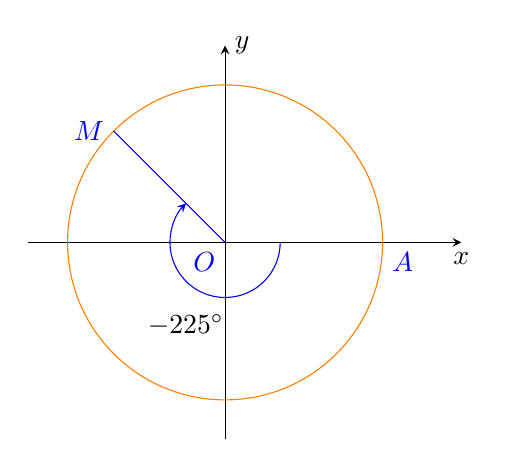
\begin{tikzpicture}		
				\draw[-stealth] (-2.5,0) -- (3,0)node[below] {$x$};
				\draw[-stealth] (0,-2.5) -- (0,2.5)node[right] {$y$};
				\draw[orange] (0,0) circle (2);
				\draw[-stealth,blue] (0:.7) arc (0:-225:.7);
				\draw[blue] (0:0) node[below left]{$O$}--(-225:2) node[left]{$M$};
				\path (-120:1) node[below=-2pt]{$-225^{\circ}$};
				\path (0:2) node[below right,blue]{$A$};
				\end{tikzpicture}
				\end{center}
		\end{enumerate}
	}
\end{bt}

\begin{bt}%[1D1H2-2]
% nguon: Archive/2024/TOAN_11_XE/TOAN_11_XE/data4/11C1/KNTT-1.1.tex #1213
%[Lê Minh Thiện Anh, dự án 11SGK-KNTT-2022]
	Tính các giá trị lượng giác của góc $\alpha$, biết
	\begin{multicols}{2}
	\begin{enumerate}
	\item $\cos\alpha=\dfrac{1}{5}$ và $0<\alpha<\dfrac{\pi}{2}$;
	\item $\sin\alpha=\dfrac{2}{5}$ và $\dfrac{\pi}{2}<\alpha<\pi$;
	\item $\tan\alpha=\sqrt{5}$ và $\pi<\alpha<\dfrac{3\pi}{2}$;
	\item $\cot\alpha=-\dfrac{1}{\sqrt{2}}$ và $\dfrac{3\pi}{2}<\alpha<2\pi$.
	\end{enumerate}
	\end{multicols}
	\loigiai{
		\begin{enumerate}
		\item Ta có $\sin^2\alpha+\cos^2\alpha=1\Rightarrow \sin^2\alpha=1-\cos^2\alpha\Leftrightarrow \hoac{& \sin\alpha=\sqrt{1-\cos^2\alpha}\\&\sin\alpha=-\sqrt{1-\cos^2\alpha}.}$\\
		Vì $0<\alpha<\dfrac{\pi}{2}$ nên $\sin\alpha>0$, suy ra $\sin\alpha=\sqrt{1-\cos^2\alpha}$\\
		$\Rightarrow\sin\alpha=\sqrt{1-\left(\dfrac{1}{5}\right)^2}=\sqrt{\dfrac{24}{25}}=\dfrac{2\sqrt{6}}{5}$.\\
		Mà $\tan\alpha=\dfrac{\sin\alpha}{\cos\alpha}$ nên $\tan\alpha=\dfrac{2\sqrt{6}}{5}:\dfrac{1}{5}=2\sqrt{6}$ và $\cot\alpha=\dfrac{\sqrt{6}}{12}$.
		\item Ta có $\sin^2\alpha+\cos^2\alpha=1\Rightarrow \cos^2\alpha=1-\sin^2\alpha\Leftrightarrow \hoac{& \cos\alpha=\sqrt{1-\sin^2\alpha}\\&\cos\alpha=-\sqrt{1-\sin^2\alpha}.}$\\
		Vì $\dfrac{\pi}{2}<\alpha<\pi$ nên $\cos\alpha<0$, suy ra $\cos\alpha=-\sqrt{1-\sin^2\alpha}$\\
		$\Rightarrow\cos\alpha=-\sqrt{1-\left(\dfrac{2}{5}\right)^2}=-\sqrt{\dfrac{21}{25}}=-\dfrac{\sqrt{21}}{5}$.\\
		Mà $\tan\alpha=\dfrac{\sin\alpha}{\cos\alpha}$ nên $\tan\alpha=\dfrac{2}{5}:\left(-\dfrac{\sqrt{21}}{5}\right)=-\dfrac{2\sqrt{21}}{21}$ và $\cot\alpha=-\dfrac{\sqrt{21}}{2}$.
		\item Vì $\pi<\alpha<\dfrac{3\pi}{2}$ nên $\cos\alpha<0$, do đó từ công thức:\\
		$1+\tan^2\alpha=\dfrac{1}{\cos^2\alpha}$, suy ra $\cos^2\alpha=\dfrac{1}{1+\tan^2\alpha}$.\\
		$\Rightarrow\cos\alpha=-\dfrac{1}{\sqrt{1+\tan^2\alpha}}=-\dfrac{1}{\sqrt{1+(\sqrt{5})^2}}=-\dfrac{\sqrt{6}}{6}$;\\ $\cot\alpha=\dfrac{1}{\tan\alpha}=\dfrac{\sqrt{5}}{5}$ và $\sin\alpha=\tan\alpha\cdot\cos\alpha=-\dfrac{\sqrt{30}}{6}$.
		\item 
		Vì $\dfrac{3\pi}{2}<\alpha<2\pi$ nên $\sin\alpha<0$, do đó từ công thức:\\
		$1+\cot^2\alpha=\dfrac{1}{\sin^2\alpha}$, suy ra $\sin^2\alpha=\dfrac{1}{1+\cot^2\alpha}$.\\
		$\Rightarrow\sin\alpha=-\dfrac{1}{\sqrt{1+\cot^2\alpha}}=-\dfrac{1}{\sqrt{1+\left(-\dfrac{1}{\sqrt{2}}\right)^2}}=-\dfrac{\sqrt{6}}{3}$;\\ $\tan\alpha=\dfrac{1}{\cot\alpha}=-\sqrt{2}$ và $\cos\alpha=\cot\alpha\cdot\sin\alpha=\dfrac{\sqrt{3}}{3}$.
		\end{enumerate}
	}
\end{bt}

\begin{bt}%[1D1H2-3]
% nguon: Archive/2024/TOAN_11_XE/TOAN_11_XE/data4/11C1/KNTT-1.1.tex #1214

	Chứng minh các đẳng thức
	\begin{multicols}{2}
		\begin{enumerate}
			\item $\cos^4\alpha-\sin^4\alpha=2\cos^2\alpha-1$;
			\item $\dfrac{\cos^2\alpha+\tan^2\alpha-1}{\sin^2\alpha}=\tan^2\alpha$.
		\end{enumerate}
	\end{multicols}
	\loigiai{
		\begin{enumerate}
		\item Ta có
		\allowdisplaybreaks
		\begin{eqnarray*}
		\cos^4\alpha-\sin^4\alpha&=& \left(\cos^2\alpha-\sin^2\alpha\right)\left(\cos^2\alpha+\sin^2\alpha\right)\\
		&= & \cos^2\alpha-\left(1-\sin^2\alpha\right)\\
		&= & 2\cos^2\alpha-1.
		\end{eqnarray*}
		\item Ta có
		\begin{eqnarray*}
		\dfrac{\cos^2\alpha+\tan^2\alpha-1}{\sin^2\alpha}&=& \dfrac{\cos^2\alpha-1}{\sin^2\alpha}+\dfrac{\tan^2\alpha}{\sin^2\alpha}\\
		&= & \dfrac{-\sin^2\alpha}{\sin^2\alpha}+\dfrac{\sin^2\alpha}{\cos^2\alpha}\cdot\dfrac{1}{\sin^2\alpha}\\
		&= & \dfrac{1}{\cos^2\alpha}-1\\
		&=&\dfrac{1-\cos^2\alpha}{\cos^2\alpha}\\
		&=&\dfrac{\sin^2\alpha}{\cos^2\alpha}=\tan^2\alpha.
		\end{eqnarray*}
		\end{enumerate}	
	}
\end{bt}

\begin{bt}%[1D1H1-6]
% nguon: Archive/2024/TOAN_11_XE/TOAN_11_XE/data4/11C1/KNTT-1.1.tex #1215

	Bánh xe của người đi xe đạp quay được $11$ vòng trong $5$ giây.
	\begin{enumerate}
	\item Tính góc (theo độ và theo radian) mà bánh xe quay được trong $1$ giây;
	\item Tính độ dài quãng đường mà người đi xe đã đi được trong $1$ phút, biết rằng đường kính của xe đạp là $680$ mm.
	\end{enumerate}
	\loigiai{
	\begin{enumerate}
	\item Trong $1$ giây, bánh xe quay được $\dfrac{11}{5}$ (vòng).\\
	Vì $1$ vòng ứng với $360^\circ$ nên góc mà bánh xe quay được trong $1$ giây là $\dfrac{11}{5}\cdot360^\circ=792^\circ$.\\
	Vì $1$ vòng ứng với $2\pi$ rad nên góc mà bánh xe quay được trong $1$ giây là $\dfrac{11}{5}\cdot2\pi=\dfrac{22\pi}{5}$(rad).
	\item Đổi $1$ phút $=60$ s.\\
	Trong $60$ giây, bánh xe quay được số vòng là $\dfrac{11}{5}\cdot60=132$ (vòng).\\
	Chu vi mỗi vòng xe là $680\pi$ (mm).\\
	Độ dài quãng đường người đó đi trong $1$ phút là $132\cdot680\pi=89760\pi$ (mm).
	\end{enumerate}	
	}
\end{bt}

\begin{bt}%[1D1H2-2]
% nguon: Archive/2024/TOAN_11_XE/TOAN_11_XE/data4/11C1/KNTT-1.1.tex #1217

	Tính các giá trị lượng giác của mỗi góc sau: $225^\circ$; $-225^\circ$; $-1~035^\circ$; $\dfrac{5\pi}{3}$; $\dfrac{19\pi}{2}$; $-\dfrac{159\pi}{4}$.
	\loigiai{
		\begin{itemize}
			\item $\sin 225^\circ=\sin (45^\circ+180^\circ)=-\sin 45^\circ=-\dfrac{\sqrt{2}}{2}$;\\
			$\cos 225^\circ=\cos (45^\circ+180^\circ)=-\cos 45^\circ=-\dfrac{\sqrt{2}}{2}$;\\
			$\tan 225^\circ=\dfrac{\sin 225^\circ}{\cos 225^\circ}=1$;
			$\cot 225^\circ=\dfrac{\cos 225^\circ}{\sin 225^\circ}=1$.
			\item $\sin (-225^\circ)=\sin (-45^\circ+180^\circ)=-\sin (-45^\circ)=\sin 45^\circ=\dfrac{\sqrt{2}}{2}$;\\
			$\cos (-225^\circ)=\cos (-45^\circ+180^\circ)=-\cos (-45^\circ)=-\cos 45^\circ=-\dfrac{\sqrt{2}}{2}$;\\
			$\tan (-225^\circ)=\dfrac{\sin (-225^\circ)}{\cos (-225^\circ)}=-1$;
			$\cot (-225^\circ)=\dfrac{\cos (-225^\circ)}{\sin (-225^\circ)}=-1$.
			\item $\sin (-1~035^\circ)=\sin (45^\circ -3\cdot 360^\circ)=\sin 45^\circ=\dfrac{\sqrt{2}}{2}$;\\
			$\cos (-1~035^\circ)=\cos (45^\circ -3\cdot 360^\circ)=\cos 45^\circ=\dfrac{\sqrt{2}}{2}$;\\
			$\tan (-1~035^\circ)=\dfrac{\sin (-1~035^\circ)}{\cos (-1~035^\circ)}=1$;
			$\cot (-1~035^\circ)=\dfrac{\cos (-1~035^\circ)}{\sin (-1~035^\circ)}=1$;	
			\item $\sin \dfrac{5\pi}{3}=\sin \left(2\pi-\dfrac{\pi}{3}\right)=\sin \left(-\dfrac{\pi}{3}\right)=-\sin \dfrac{\pi}{3}=-\dfrac{\sqrt{3}}{2}$;\\
			$\cos \dfrac{5\pi}{3}=\cos \left(2\pi-\dfrac{\pi}{3}\right)=\cos \left(-\dfrac{\pi}{3}\right)=\cos \dfrac{\pi}{3}=\dfrac{1}{2}$;\\
			$\tan \dfrac{5\pi}{3}=\dfrac{\sin \dfrac{5\pi}{3}}{\cos \dfrac{5\pi}{3}}=-\sqrt{3}$;
			$\cot \dfrac{5\pi}{3}=\dfrac{\cos \dfrac{5\pi}{3}}{\sin \dfrac{5\pi}{3}}=-\dfrac{\sqrt{3}}{3}$.
			\item $\sin \dfrac{19\pi}{2}=\sin \left(10\pi-\dfrac{\pi}{2}\right)=\sin \left(-\dfrac{\pi}{2}\right)=-\sin \dfrac{\pi}{2}=-1$;\\
			$\cos \dfrac{19\pi}{2}=\cos \left(10\pi-\dfrac{\pi}{2}\right)=\cos \left(-\dfrac{\pi}{2}\right)=\cos \dfrac{\pi}{2}=0$;
			$\cot \dfrac{19\pi}{2}=\dfrac{\cos \dfrac{19\pi}{2}}{\sin \dfrac{19\pi}{2}}=0$.
			\item $\sin \left(-\dfrac{159\pi}{4}\right)=\sin \left(\dfrac{\pi}{4}-40\pi\right)=\sin \dfrac{\pi}{4}=\dfrac{\sqrt{2}}{2}$;\\
			$\cos \left(-\dfrac{159\pi}{4}\right)=\cos \left(\dfrac{\pi}{4}-40\pi\right)=\cos \dfrac{\pi}{4}=\dfrac{\sqrt{2}}{2}$;\\
			$\tan \left(-\dfrac{159\pi}{4}\right)=\dfrac{\sin \left(-\dfrac{159\pi}{4}\right)}{\cos \left(-\dfrac{159\pi}{4}\right)}=1$;
			$\cot \left(-\dfrac{159\pi}{4}\right)=\dfrac{\cos \left(-\dfrac{159\pi}{4}\right)}{\sin \left(-\dfrac{159\pi}{4}\right)}=1$.
		\end{itemize}
	}
\end{bt}

\begin{bt}%[1D1V2-2]
% nguon: Archive/2024/TOAN_11_XE/TOAN_11_XE/data4/11C1/KNTT-1.1.tex #1218

	Tính các giá trị lượng giác (nếu có) của mỗi góc sau
	\begin{listEX}[2]
		\item $\dfrac{\pi}{3}+k2\pi$ ($k\in \mathbb{Z}$);
		\item $k\pi$ ($k\in \mathbb{Z}$);
		\item $\dfrac{\pi}{2}+k\pi$ ($k\in \mathbb{Z}$);
		\item $\dfrac{\pi}{4}+k\pi$ ($k\in \mathbb{Z}$).
	\end{listEX}
	\loigiai{\begin{multicols}{2}	
			\begin{enumerate}
				\item Xét $\alpha=\dfrac{\pi}{3}+k2\pi$ ($k\in \mathbb{Z}$), ta có
				\begin{itemize}
					\item $\sin \alpha=\sin \dfrac{\pi}{3}=\dfrac{\sqrt{3}}{2}$;
					\item $\cos \alpha=\cos \dfrac{\pi}{3}=\dfrac{1}{2}$;
					\item $\tan \alpha=\tan \dfrac{\pi}{3}=\sqrt{3}$;
					\item $\cot \alpha=\tan \dfrac{\pi}{3}=\dfrac{\sqrt{3}}{3}$.
				\end{itemize}
				\item Xét $\alpha=k\pi$ ($k\in \mathbb{Z}$), ta có
				\begin{itemize}
					\item $\sin \alpha=0$;
					\item $\cos \alpha=(-1)^k$;
					\item $\tan \alpha=0$;
					\item $\cot \alpha$ không xác định.
				\end{itemize}
				\item Xét $\alpha=\dfrac{\pi}{2}+k\pi$ ($k\in \mathbb{Z}$), ta có
				\begin{itemize}
					\item $\sin \alpha=(-1)^k$;
					\item $\cos \alpha=0$;
					\item $\cot \alpha=0$;
					\item $\tan \alpha$ không xác định.
				\end{itemize}
				\item Xét $\alpha=\dfrac{\pi}{4}+k\pi$ ($k\in \mathbb{Z}$), ta có
				\begin{itemize}
					\item $\sin \alpha=(-1)^k\cdot \dfrac{\sqrt{2}}{2}$;
					\item $\cos \alpha=(-1)^k\cdot \dfrac{\sqrt{2}}{2}$;
					\item $\tan \alpha=1$;
					\item $\cot \alpha=1$.
				\end{itemize}
			\end{enumerate}
		\end{multicols}
	}
\end{bt}

\begin{bt}%[1D1H2-2]
% nguon: Archive/2024/TOAN_11_XE/TOAN_11_XE/data4/11C1/KNTT-1.1.tex #1219

	Tính các giá trị lượng giác của góc $\alpha$ trong mỗi trường hợp sau
	\begin{listEX}[2]
		\item $\sin \alpha=\dfrac{\sqrt{15}}{4}$ với $\dfrac{\pi}{2}<\alpha<\pi$;
		\item $\cos \alpha=-\dfrac{2}{3}$ với $-\pi<\alpha<0$;
		\item $\tan \alpha=3$ với $-\pi<\alpha<0$;
		\item $\cot \alpha=-2$ với $0<\alpha<\pi$.
	\end{listEX}
	\loigiai{
		\begin{enumerate}
			\item Xét $\sin \alpha=\dfrac{\sqrt{15}}{4}$ với $\dfrac{\pi}{2}<\alpha<\pi$;\\
			Vì $\sin^2\alpha+\cos^2\alpha=1$ nên $\cos^2\alpha=1-\sin^2\alpha=1-\left(\dfrac{\sqrt{15}}{4}\right)^2=\dfrac{1}{16}$.\\
			Do $\dfrac{\pi}{2}<\alpha<\pi$ nên $\cos \alpha<0$.\\
			Từ đó ta có $\cos \alpha=-\sqrt{\dfrac{1}{16}}=-\dfrac{1}{4}$.\\
			Ta có $\tan \alpha=\dfrac{\sin \alpha}{\cos \alpha}=-\sqrt{15}$; $\cot \alpha=\dfrac{\cos \alpha}{\sin \alpha}=-\dfrac{\sqrt{15}}{15}$.
			\item Xét $\cos \alpha=-\dfrac{2}{3}$ với $-\pi<\alpha<0$;\\
			Vì $\sin^2\alpha+\cos^2\alpha=1$ nên $\sin^2\alpha=1-\cos^2\alpha=1-\left(-\dfrac{2}{3}\right)^2=\dfrac{5}{9}$.\\
			Do $-\pi<\alpha<0$ nên $\sin \alpha<0$.\\
			Từ đó ta có $\sin \alpha=-\sqrt{\dfrac{5}{9}}=-\dfrac{\sqrt{5}}{3}$.\\
			Ta có $\tan \alpha=\dfrac{\sin \alpha}{\cos \alpha}=-\dfrac{\sqrt{5}}{2}$; $\cot \alpha=\dfrac{\cos \alpha}{\sin \alpha}=-\dfrac{2\sqrt{5}}{5}$.
			\item Xét $\tan \alpha=3$ với $-\pi<\alpha<0$;\\
			Ta có $\cot \alpha=\dfrac{1}{3}$.\\
			Do $\tan \alpha=3$ nên $\dfrac{\sin \alpha}{\cos \alpha}=3$, suy ra $\sin \alpha=3\cos \alpha$.\\
			Vì $\cos^2\alpha+\sin^2\alpha=1$ nên $\cos^2\alpha+(3\cos\alpha)^2=1$, suy ra $\cos^2 \alpha=\dfrac{1}{10}$.
			\begin{itemize}
				\item Do $-\dfrac{\pi}{2}<\alpha<0$ nên $\cos \alpha>0$.\\
				Từ đó ta có $\cos \alpha=\dfrac{\sqrt{10}}{10}$.
				\item Do $-\pi<\alpha<-\dfrac{\pi}{2}$ nên $\cos \alpha<0$.\\
				Từ đó ta có $\cos \alpha=-\dfrac{\sqrt{10}}{10}$.
			\end{itemize}
			\item Xét $\cot \alpha=-2$ với $0<\alpha<\pi$;\\
			Ta có $\tan \alpha=-\dfrac{1}{2}$.\\
			Do $\cot \alpha=-2$ nên $\dfrac{\cos \alpha}{\sin \alpha}=-2$, suy ra $\cos \alpha=-2\sin \alpha$.\\
			Vì $\cos^2\alpha+\sin^2\alpha=1$ nên $(-2\sin \alpha)^2+\sin^2\alpha=1$, suy ra $\sin^2 \alpha=\dfrac{1}{5}$.\\
			Do $0<\alpha<\pi$ nên $\sin \alpha>0$.\\
			Từ đó ta có $\sin \alpha=\dfrac{\sqrt{5}}{5}$.
		\end{enumerate}
	}
\end{bt}

\begin{bt}%[1D1V2-4]
% nguon: Archive/2024/TOAN_11_XE/TOAN_11_XE/data4/11C1/KNTT-1.1.tex #1220

	Tính
	\begin{enumerate}
		\item $A=\sin^2 5^\circ+\sin^2 10^\circ+\sin^2 15^\circ+\ldots+\sin^2 85^\circ$ ($17$ số hạng);
		\item $B=\cos 5^\circ+\cos 10^\circ+\cos 15^\circ+\ldots+\cos 175^\circ$ ($35$ số hạng).
	\end{enumerate}
	\loigiai{
		\begin{enumerate}
			\item Nhận xét thấy $\sin^2 85^\circ=\left[\sin (90^\circ-5^\circ)\right]^2=\cos^2 5^\circ$.\\
			Do đó
			\begin{eqnarray*}
				A&=&\sin^2 5^\circ+\sin^2 10^\circ+\sin^2 15^\circ+\ldots+\sin^2 85^\circ\\
				&=&\sin^2 5^\circ+\sin^2 85^\circ+\sin^2 10^\circ+\sin^2 80^\circ+\ldots+\sin^2 45^\circ\\
				&=&\sin^2 5^\circ+\cos^2 5^\circ+\sin^2 10^\circ+\cos^2 10^\circ+\ldots+\sin^2 45^\circ\\
				&=&\underbrace {1+1+\ldots+1}_{8\text{ số hạng}}+\dfrac{1}{2}=\dfrac{17}{2}.
			\end{eqnarray*}
			\item Nhận xét thấy $\cos 175^\circ=\cos (180^\circ-5^\circ)=-\cos 5^\circ$.\\
			Do đó
			\begin{eqnarray*}
				B&=&\cos 5^\circ+\cos 10^\circ+\cos 15^\circ+\ldots+\cos 175^\circ\\
				&=&\cos 5^\circ+\cos 175^\circ+\cos 10^\circ+\cos 170^\circ+\ldots+\cos 90^\circ\\
				&=&\cos 5^\circ-\cos 5^\circ+\cos 10^\circ-\cos10^\circ+\ldots+\cos 90^\circ\\
				&=&\cos 90^\circ\\
				&=&0.
			\end{eqnarray*}
		\end{enumerate}
	}
\end{bt}

\begin{bt}%[1D1H5-6]
% nguon: Archive/2024/SP-K10-K11-LyVanHoang_TVN-023/11. C1-LuongGiac-lvhoang_TVN-023/dataC1K11/Chuong1-Bai4-Dang6-Toanthucte-lienmon.tex #1701
[CTST]%[Anh Duy]
	\immini{Trong hình bên, khi bàn đạp xe đạp quay, bóng $M$ của đầu trục quay dao động trên mặt đất quanh điểm $O$ theo phương trình $s=17\cos5\pi t$ với $s$ $(\mathrm{cm})$ là toạ độ của điểm $M$ trên trục $Ox$ và $t$ (giây) là thời gian bàn đạp quay. Xác định các thời điểm mà tại đó độ dài bóng $OM$ bằng $10$ $\mathrm{cm}$?}{
	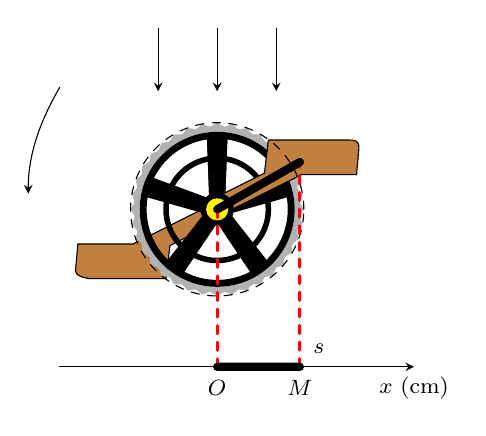
\begin{tikzpicture}[line join = round, line cap=round,>=stealth,font=\footnotesize,scale=1]
		
		\draw[fill=brown] 
		(0, 0) -- (0, -0.16) -- (-0.6, -0.46) -- (-0.65, -0.88) -- (-1.65, -0.88)
		.. controls +(180:-0.1) and +(-90:0.1) .. (-1.8, -0.78) -- (-1.77, -0.44) 
		-- (-1.07, -0.44) -- (-0.07, 0.06) -- cycle;	
		
		\foreach \x in {0,-10,...,-350}
		\fill[black!30!white,rotate=\x] 
		(95:1.05)--(90:1.1)--(85:1.05)--cycle;
		\draw[black!30!white,line width=2pt] (0,0) circle(1.02cm);
		
		\draw[black,line width=2.5pt](0,0) circle(0.94cm);	
		\draw[black,line width=2pt](0,0) circle(0.65cm);
		
		\foreach \x in{0,72,144,216,288,360}
		\fill[line width=1pt,rotate=\x] 
		(0, 0) -- (0.1, 0.1) -- (0.13, 0.9) --(-0.13, 0.9) -- (-0.1, 0.1) -- (0, 0);
		
		\draw[fill=brown] 
		(0, 0) -- (0, 0.16) -- (0.6, 0.46) -- (0.65, 0.88) -- (1.65, 0.88)
		.. controls +(0:0.1) and +(90:0.1) .. (1.8, 0.78) -- (1.77, 0.44) 
		-- (1.07, 0.44) -- (0.07, -0.06) -- cycle	
		;
		
		\draw[dashed] (0,0) circle(1.1cm);
		
		\fill[black](0,0) circle(6pt);
		\fill[yellow] (0,0) circle(4pt);
		
		\draw[red,dashed,line width=1pt] 
		(0,0)--(0,-2)
		(1.05,-2)--(1.05,0.6)
		;
		\draw[black,line width=3pt] (0,0)--(1.05,0.6) (0,-2)node[below]{$O$}--(1.05,-2)node[above right]{$s$}node[below]{$M$};
		\draw[->](-2,-2)--(2.5,-2) node[below]{$x$ (cm)};
		
		\draw[->] (-2,1.55)..controls +(-120:0.5) and +(90:0.5) .. (-2.4,0.2);
		\draw[->] (-0.75,2.3)--(-0.75,1.5);\draw[->] (-0,2.3)--(-0,1.5); \draw[->] (0.75,2.3)--(0.75,1.5);
		
		\end{tikzpicture}}
	\loigiai{
		Độ dài bóng $OM$ bằng $10$ $\mathrm{cm}$ khi và chỉ khi
		\begin{eqnarray*}
			&&\hoac{&17\cos5\pi t=10\\&17\cos5\pi t=-10}\Leftrightarrow\hoac{&\cos5\pi t=\dfrac{10}{17}\\&\cos5\pi t=-\dfrac{10}{17}}\\&\Leftrightarrow&\hoac{&5\pi t=\pm\arccos\dfrac{10}{17}+k2\pi\\&5\pi t=\pm\arccos\left(-\dfrac{10}{17}\right)+k2\pi}\\&\Leftrightarrow&\hoac{&t=\pm\dfrac{1}{5\pi}\arccos\dfrac{10}{17}+\dfrac{2k}{5}\\&t=\pm\dfrac{1}{5\pi}\arccos\left(-\dfrac{10}{17}\right)+\dfrac{2k}{5}},\,k\in\mathbb{Z}.	
		\end{eqnarray*}
	}
\end{bt}

\begin{bt}%[1D1H5-6]
% nguon: Archive/2024/SP-K10-K11-LyVanHoang_TVN-023/11. C1-LuongGiac-lvhoang_TVN-023/dataC1K11/Chuong1-Bai4-Dang6-Toanthucte-lienmon.tex #1707
%[Anh Duy]
	Trong hình dưới, ngọn đèn trên hải đăng $H$ cách bờ biển $y y'$ một khoảng $HO=1$ km. Đèn xoay ngược chiều kim đồng hồ với tốc độ $\dfrac{\pi}{10}$ rad/s và chiếu hai luồng ánh sáng về hai phía đối diện nhau. Khi đèn xoay, điểm $M$ mà luồng ánh sáng của hải đăng rọi vào bờ biển chuyển động dọc theo bờ.
	\begin{center}
		
\begin{tikzpicture}[scale=1.3,font=\footnotesize, line join=round, line cap=round, >=stealth]
			\definecolor{nen tron}{RGB}{173,223,246}
			\definecolor{thap trai}{rgb}{0.51, 0.21, 0.21}
			\definecolor{thap mat}{rgb}{0.51, 0.21, 0.30}
			\definecolor{luon duoi}{RGB}{1,116,181}
			\fill[black!40] (-2.5,-2.3) rectangle (2.5,3.2);
			% NữaTháp phải
			\fill[black!20] (0,-1.7) ellipse (2 and .5); 
			\def \A{
				(0,2)
				..controls +(-90:.1) and +(150:.12)..(.07,1.46)
				..controls +(-60:.1) and +(90:.1)..(.11,1.32)
				--(.52,1.11)--(.52,1.08)--(.4,1.08)--(.4,.72)--(.48,.72)--(.48,.6)--(.4,.6)
				--(.6,-1.49)--(0,-1.49)--(0,2)}
			\fill[thap mat] \A;
			\fill[thap trai][xscale=-1] \A;
			% Ô cửa phải
			\def\B{
				(.11,.76)--(.26,.76)--(.26,1.04)--(.11,1.04)--(.11,.76) 
				(0,.76)--(.07,.76)--(.07,1.04)--(0,1.04)--(0,.76)}
			\fill[nen tron]\B;
			\fill[nen tron][xscale=-1] \B;
			% chân tháp
			\fill[thap mat] 
			(0,-1.49)--(.7,-1.49)--(.72,-1.6)--(0,-1.6);
			\fill[thap trai]
			(0,-1.49)--(0,-1.6)
			..controls +(175:.3) and +(3:.1)..(-.72,-1.58) --(-.71,-1.49)
			--(0,-1.49);
			
			\foreach \a in {0, 20, ..., 360}{%
				\begin{scope}[shift={(0,1.8)}]
					\fill[rotate=\a,white] (0,0)--(0,1);
					\fill[rotate=45,white] (-1.5,0)--(0,0.03)--(1.5,0)--(0,-0.03)--(-1.5,0);
				\end{scope}
			}
			\fill [white] (0,1.8) circle (.2);
			
		\end{tikzpicture} \hspace{2cm}
		\begin{tikzpicture}[scale=1,font=\footnotesize, line join=round, line cap=round, >=stealth]
			\path 
			(0,0) coordinate (O)
			(-3,0) coordinate (H)
			(0,2) coordinate (M)
			(0,-3) coordinate (N)
			
			;
			
			\draw[->] (0,-4) -- (0,3)node[right] {$y$};
			\draw[blue,shorten >=-2cm] (M)--(H);
			\draw[dashed] (H)--(O);
			\draw pic[draw, angle radius=2mm]{right angle=H--O--M};
			\pic[draw,"$\alpha$", angle eccentricity=0.6,angle radius=0.8cm]{angle=O--H--M};
			\path (O)--(N) node[right,midway]{$1$ km};
			\path (O)--(H) node[below,midway]{$1$ km};
			\path (0,-4) node[left]{$y'$};
			\path (0,-4) node[right]{bờ biển};
			\foreach \x/\g in {H/90,O/0,N/0,M/0} \fill[black] (\x) circle (1pt)+(\g:.3) node {$\x$};
			%%\path ([xshift=-.25cm]current bounding box.south) node[below]{\HINHVE};
		\end{tikzpicture}
	\end{center}
	\begin{enumerate}[a)]
		\item Ban đầu luồng sáng trùng với đường thẳng $HO$. Viết hàm số biểu thị toạ độ $y_M$ của điểm $M$ trên trục $Oy$ theo thời gian $t$.
		\item Ngôi nhà $N$ nằm trên bờ biển với toạ độ $y_N=-1$ (km). Xác định các thời điểm $t$ mà đèn hải đăng chiếu vào ngôi nhà.
	\end{enumerate}
	\loigiai{
		\begin{enumerate}[a)]
			\item Xét $\triangle OMH$ có 
			$OM=OH\cdot \tan \alpha\Rightarrow y_M=\tan \alpha=\tan \left(\dfrac{\pi t}{10}\right)$.\\
			Vậy hàm số biểu thị toạ độ $y_M$ của điểm $M$ trên trục $Oy$ theo thời gian $t$ là $y_M=\tan \left(\dfrac{\pi t}{10}\right)$.
			\item Theo giả thiết, ta có \allowdisplaybreaks
			\begin{eqnarray*}
				&&y_N=-1\\
				&\Leftrightarrow& \tan \left(\dfrac{\pi t}{10}\right)=-1\\
				&\Leftrightarrow& \dfrac{\pi t}{10}=-\dfrac{\pi}{4}+k\pi\\ &\Leftrightarrow&  t=-\dfrac{5}{2}+10k \,(k\in \mathbb{N}^*).
			\end{eqnarray*}
		\end{enumerate}
		
	}
\end{bt}

\begin{bt}%[1D1N1-3]
% nguon: Archive/2024/SP-K10-K11-LyVanHoang_TVN-023/11. C1-LuongGiac-lvhoang_TVN-023/dataC1K11/Bai1-Dang2.tex #1950
%[TeX hóa CD 11]%[Nhật Thiện]
	Cho góc lượng giác $(Ou,Ov)$ có số đo là $-\dfrac{11\pi}{4}$, góc lượng giác $(Ou,Ow)$ có số đo là $\dfrac{3\pi}{4}$. Tìm số đo của góc lượng giác $(Ov,Ow)$.
	\loigiai{
		Theo hệ thức Chasles, ta có
		\begin{eqnarray*}
			(Ov,Ow)&=&(Ou,Ow)-(Ou,Ov)+k2\pi\\
			&=&\dfrac{3\pi}{4}+\dfrac{11\pi}{4}+k2\pi\\
			&=&\dfrac{7\pi}{2}+k2\pi\ (k\in \mathbb{Z}).
		\end{eqnarray*}
	}
\end{bt}

\begin{bt}%[1D1V4-2]
% nguon: Archive/SP_KhoLatex/ID6_old/1-GK1-KNTT-De15-NH23-24.tex #2709

	Tìm tập xác định của hàm số $y=\dfrac{\sqrt{1+\cos{2x}}}{1-\left(\sin x-\cos x\right)^2}$.
	\loigiai{
	Hàm số xác định khi và chỉ khi $\heva{&1+\cos{2x}\geq0\\&1-\left(\sin x-\cos x\right)^2\neq0} \Leftrightarrow \heva{&\cos{2x}\geq-1\\&\sin{2x}\neq0}$.\\
	$\cos{2x}\geq-1$ thỏa mãn $\forall x\in\mathbb{R}$.\\
	$\sin{2x}\neq0 \Leftrightarrow 2x\neq k\pi,k\in\mathbb{Z} \Leftrightarrow x\neq k\dfrac{\pi}{2},k\in\mathbb{Z}$.\\
	Vậy tập xác định của hàm số là $\mathscr{D}=\mathbb{R}\setminus\left\{k\dfrac{\pi}{2},k\in\mathbb{Z}\right\}$.
	}
\end{bt}

\begin{bt}%[1D1V5-5]
% nguon: Archive/SP_KhoLatex/ID6_old/1-GK1-KNTT-De15-NH23-24.tex #2710

	Giải phương trình $\sin\left(\dfrac{\pi}{6}+x\right)=\cos{2x}$. 
	\loigiai{
		Ta có $\sin\left(\dfrac{\pi}{6}+x\right)=\cos{2x} \Leftrightarrow \sin\left(\dfrac{\pi}{6}+x\right)=\sin\left(\dfrac{\pi}{2}-2x\right)$\\
		$\Leftrightarrow \hoac{&\dfrac{\pi}{6}+x=\dfrac{\pi}{2}-2x+k2\pi\\&\dfrac{\pi}{6}+x=\pi-\left(\dfrac{\pi}{2}-2x\right)+k2\pi}$ $\Leftrightarrow \hoac{&x=\dfrac{\pi}{9}+k\dfrac{2\pi}{3}\\&x=-\dfrac{\pi}{3}+k2\pi},k\in\mathbb{Z}$.
	}
\end{bt}

\begin{bt}%[1D1H4-8]
% nguon: Archive/SP_KhoLatex/ID6_old/1-GK1-CanhDieu-De5-NH23-24.tex #2743
%[Pj17-0-CK2-NH22-23--TeamTeXHoa--VoVanTu]
	Tại một cửa biển, mực nước con sông đổ ra biển trong một ngày theo quy luật $h(t)=\cos \left(\dfrac{\pi}{2} t+\dfrac{\pi}{6}\right)$ và mực nước biển cùng thời điểm theo quy luật $H(t)=\cos \left(\dfrac{\pi}{4} t+\dfrac{\pi}{3}\right)$ ($t$ là thời gian trong ngày, đơn vị là giờ $(h)$, mực nước tính theo đơn vị mét $(m)$). Để ngăn sự xâm mặn của nước biển gây ảnh hưởng đến canh tác của nông dân, người ta xây một hệ thống chắn tự động, nó sẽ đóng hoặc mở khi mực nước của sông và biển bằng nhau. Hỏi mỗi ngày hệ thống đóng-mở bao nhiêu lần.
	\loigiai{
	Khi mực nước của sông và biển bằng nhau, ta có
	$$
	\cos \left(\dfrac{\pi}{2} t+\dfrac{\pi}{6}\right)=\cos \left(\dfrac{\pi}{4} t+\dfrac{\pi}{3}\right).
	$$
	Đặt $x=\dfrac{\pi t}{4} ; t \in[0 ; 24] \Rightarrow x \in[0 ; 6]$.\\	
	Ta có phương trình
	$$\cos \left(2 x+\dfrac{\pi}{6}\right)=\cos \left(x+\dfrac{\pi}{3}\right) \Leftrightarrow\hoac{&2 x+\dfrac{\pi}{6}=x+\dfrac{\pi}{3}+k 2 \pi \\ &2 x+\dfrac{\pi}{6}=-x-\dfrac{\pi}{3}+k 2 \pi} \Leftrightarrow\hoac{&x=\dfrac{\pi}{6}+k 2 \pi \\ &x=-\dfrac{\pi}{6}+\dfrac{k 2 \pi}{3}}~(k \in \mathbb{Z}).$$
	\begin{itemize}
		\item Với $x=\dfrac{\pi}{6}+k 2 \pi \Rightarrow 0 \leq \dfrac{\pi}{6}+k 2 \pi \leq 6 \Leftrightarrow-\dfrac{1}{12} \leq k \leq \dfrac{6}{2 \pi}-\dfrac{1}{12} \approx 0{,}87 \Rightarrow k=0$.
		\item Với $x=-\dfrac{\pi}{6}+\dfrac{k 2 \pi}{3} \Rightarrow 0 \leq-\dfrac{\pi}{6}+\dfrac{k 2 \pi}{3} \leq 6 \Leftrightarrow \dfrac{1}{4} \leq k \leq \dfrac{9}{\pi}+\dfrac{1}{4} \approx 3{,}11 \Rightarrow k \in\{1 ; 2 ; 3\}$.\\ Vậy mỗi ngày hệ thống đóng-mở $4$ lần.
	\end{itemize}
}
\end{bt}

\begin{bt}%[1D1H3-2]
% nguon: Archive/SP_KhoLatex/ID6_old/1-GK1-CTST-De10-NH23-24.tex #2754
%[Câu 36]
	Cho $\tan \left(a+b\right)=7$ và $\tan \left(a-b\right)=4$. Tính $\tan 2a$
\loigiai{
	Ta có $\tan 2a=\tan \left[\left(a+b\right)+\left(a-b\right)\right]=\dfrac{\tan \left(a+b\right)+\tan \left(a-b\right)}{1-\tan \left(a+b\right).\tan \left(a-b\right)}=\dfrac{7+4}{1-7.4}=-\dfrac{11}{27}$.}
\end{bt}

\begin{bt}%[1D1V3-2]
% nguon: Archive/SP_KhoLatex/ID6_old/1-GK1-CTST-De10-NH23-24.tex #2756
%[Câu 38]
	Trong hình $3$, tam giác $ABC$ vuông tại $B$ và có hai cạnh góc vuông là \break $AB=4,BC=3$. Vẽ điểm $D$ nằm trên tia đối của tia $CB$ thoả mãn $\widehat{CAD}=30^\circ$. Tính $\text{tan}\widehat{BAD}$, từ đó tính độ dài cạnh $CD$
\loigiai{	
	\begin{center}
		\begin{tikzpicture}[>=stealth,line join=round,line cap=round,font=\footnotesize,scale=1]
			\path (0,0) coordinate (B)
			(0,2) coordinate (A)
			(1.5,0) coordinate (C)
			(4,0) coordinate (D);
			\draw (A)--(B)--(D)--cycle (A)--(C);
			\path pic[angle radius=5mm,draw=blue,fill=green,"$30^\circ$",angle eccentricity=1.5] {angle = C--A--D};
			\path pic[angle radius=3mm,draw=blue,fill=green] {right angle = A--B--C};
			\path (B)--(A)node[pos=0.5,sloped,black,above]{$4$};
			\path (B)--(C)node[pos=0.5,sloped,black,below]{$3$};
			\foreach \t/\g in {A/90,B/180,C/-90,D/0}{
				\draw[fill=white] (\t) circle (1pt) node[shift={(\g:7pt)},font=\scriptsize]{$ \t $};
			}
		\end{tikzpicture}
	\end{center}
	Xét tam giác $ABC$ vuông tại $B$ có: $\text{tan}\widehat{BAC}=\dfrac{3}{4}$.\\
	Ta lại có $\widehat{BAD}=\widehat{BAC}+\widehat{CAD}$, suy ra
	\begin{eqnarray*}
	\tan \widehat{BAD} &=& \tan \left(\widehat{BAC}+\widehat{CAD} \right)\\
	&=& \tan \left(\widehat{BAC}+30^\circ \right)\\
	&=& \dfrac{\tan \widehat{BAC}+\tan 30^\circ}{1-\tan \widehat{BAC} \cdot \tan 30^\circ}\\
	&=& \dfrac{\dfrac{3}{4}+\dfrac{\sqrt{3}}{3}}{1-\dfrac{3}{4}\cdot \dfrac{\sqrt{3}}{3}}=\dfrac{48+25\sqrt{3}}{39}\approx 2{,}34.		
	\end{eqnarray*}
}
\end{bt}

\begin{bt}%[1D1H6-3]
% nguon: Archive/SP_KhoLatex/ID6_old/1K1-4-9.tex #2983
[TH]%[DCHT Toán 11 - KNTT -Tên Nguyễn Thanh Sang] 
	Giải phương trình: $\sin x + \sqrt{3}\cos x=1$. 
	\dapso{$\left\{ -\dfrac{\pi}{6} +  2k\pi; \dfrac{\pi}{2}+2k\pi, k\in\mathbb{Z}  \right\}$.}
	\loigiai{
		Điều kiện $1^2 + \left(\sqrt{3}\right)^2=4>1^2$ (luôn đúng).\\
		Chia $2$ vế cho $\sqrt{a^2 + b^2}=2$ thì phương trình trở thành:
		\begin{eqnarray*}
			& & \dfrac{1}{2}\sin x + \dfrac{\sqrt{3}}{2}\cos x= \dfrac{1}{2}\\
			&\Leftrightarrow & \sin x\cos\dfrac{\pi}{3} + \cos x\sin\dfrac{\pi}{3} = \sin\dfrac{\pi}{6} \\
			&\Leftrightarrow & \sin\left(x + \dfrac{\pi}{3}\right)=\sin \dfrac{\pi}{6}\\
			&	\Leftrightarrow & \hoac{&x+\dfrac{\pi}{3} = \dfrac{\pi}{6}+ k2\pi\\&x + \dfrac{\pi}{3} = \pi - \dfrac{\pi}{6} + 2k\pi  } \\
			&	\Leftrightarrow & \hoac{&x = -\dfrac{\pi}{6} +  2k\pi\\&x = \dfrac{\pi}{2}+2k\pi.}
		\end{eqnarray*}
		Kết luận $S= \left\{ -\dfrac{\pi}{6} +  2k\pi; \dfrac{\pi}{2}+2k\pi \mid k\in\mathbb{Z}  \right\}$.
		}
\end{bt}

\begin{bt}%[1D1V6-3]
% nguon: Archive/SP_KhoLatex/ID6_old/1K1-4-9.tex #2984
[TH]%[DCHT Toán 11 - KNTT -Tên Nguyễn Thanh Sang] 
Giải phương trình: $\sqrt{3}\cos x - \sin x=\sqrt{2}$.
\dapso{$S= \left\{\dfrac{\pi}{12} +  2k\pi; -\dfrac{5\pi}{12}+2k\pi\mid k\in\mathbb{Z}  \right\}$.}
\loigiai{
	Điều kiện $\left(\sqrt{3}\right)^2 + (-1)^2 = 4>\left(\sqrt{2}\right)^2$ (luôn đúng).\\
	Chia $2$ vế cho $\sqrt{a^2 + b^2}=2$ thì phương trình trở thành
	\begin{eqnarray*}
		& & \dfrac{\sqrt{3}}{2}\cos x - \dfrac{1}{2}\sin x= \dfrac{\sqrt{2}}{2}\\
		&\Leftrightarrow & \cos x\cdot \cos\dfrac{\pi}{6} - \sin x\cdot \sin\dfrac{\pi}{6} = \cos\dfrac{\pi}{4} \\
		&\Leftrightarrow & \cos\left(x + \dfrac{\pi}{6}\right)=\cos\dfrac{\pi}{4}\\
		&	\Leftrightarrow & \hoac{&x+\dfrac{\pi}{6} = \dfrac{\pi}{4}+ k2\pi\\&x + \dfrac{\pi}{6} = -\dfrac{\pi}{4} + 2k\pi  } \\
		&	\Leftrightarrow & \hoac{&x = \dfrac{\pi}{12} +  2k\pi\\&x = -\dfrac{5\pi}{12}+2k\pi.}
	\end{eqnarray*}
	Kết luận $S= \left\{\dfrac{\pi}{12} +  2k\pi; -\dfrac{5\pi}{12}+2k\pi\mid k\in\mathbb{Z}  \right\}$.
}
\end{bt}

\begin{bt}%[1D1V6-3]
% nguon: Archive/SP_KhoLatex/ID6_old/1K1-4-9.tex #2985
[TH]%[DCHT Toán 11 - KNTT -Tên Nguyễn Thanh Sang] 
	 Giải phương trình: $\sqrt{3}\sin{2x} + \cos{2x}=\sqrt{2}$.
	\dapso{$S= \left\{ \dfrac{\pi}{24} +  k\pi; \dfrac{7\pi}{24}+k\pi\mid k\in\mathbb{Z}  \right\}$}
	 \loigiai{
	 	Điều kiện $\left(\sqrt{3}\right)^2 + 1^2 = 4>\left(\sqrt{2}\right)^2$ (luôn đúng).\\
	 	Chia $2$ vế cho $\sqrt{a^2 + b^2}=2$ thì phương trình trở thành
	 	\begin{eqnarray*}
	 		& & \dfrac{\sqrt{3}}{2}\sin 2x + \dfrac{1}{2}\cos 2x= \dfrac{\sqrt{2}}{2}\\
	 		&\Leftrightarrow & \sin 2x\cdot \cos\dfrac{\pi}{6} + \cos 2x\cdot \sin\dfrac{\pi}{6} = \sin\dfrac{\pi}{4} \\
	 		&\Leftrightarrow & \sin\left(2x + \dfrac{\pi}{6}\right)=\sin\dfrac{\pi}{4}\\
	 		&	\Leftrightarrow & \hoac{&2x+\dfrac{\pi}{6} = \dfrac{\pi}{4}+ k2\pi\\&2x + \dfrac{\pi}{6} = \pi -\dfrac{\pi}{4} + 2k\pi  } \\
	 		&	\Leftrightarrow & \hoac{&x = \dfrac{\pi}{24} +  k\pi\\&x = \dfrac{7\pi}{24}+k\pi.}
	 	\end{eqnarray*}
	 	Kết luận $S= \left\{ \dfrac{\pi}{24} +  k\pi; \dfrac{7\pi}{24}+k\pi\mid k\in\mathbb{Z}  \right\}$.
} 	
\end{bt}

\begin{bt}%[1D1V6-7]
% nguon: Archive/SP_KhoLatex/ID6_old/1K1-4-9.tex #2986
[VDT]%[DCHT Toán 11 - KNTT -Tên Nguyễn Thanh Sang] 
Tìm tất cả các giá trị nguyên của $m$ để phương trình $(m-1)\sin 2x-4\cos 2x=2-2m$ có nghiệm.
	\dapso{$-1, 0, 1, 2, 3.$}
\loigiai{
		Để phương trình có nghiệm thì \begin{eqnarray*}
		& &(m-1)^2+(-4)^2\ge (2-2m)^2\\
		&\Leftrightarrow& m^2-2m+1+16\ge 4-8m+4m^2\\
		&\Leftrightarrow& 3m^2-6m-13\le 0\\
		&\Leftrightarrow& \dfrac{3-4\sqrt{3}}{3}\le m\le \dfrac{3+4\sqrt{3}}{3}.
	\end{eqnarray*}
	Khi đó các giá trị nguyên của tham số $m$ là $-1$, $0$, $1$, $2$, $3$.
	}
\end{bt}

\begin{bt}%[1D1V6-7]
% nguon: Archive/SP_KhoLatex/ID6_old/1K1-4-9.tex #2987
[VDT]%[DCHT Toán 11 - KNTT -Tên Nguyễn Thanh Sang] 
	Tính tổng tất cả các giá trị nguyên của tham số $m$ để phương trình $(2m+1)\sin x-(m+2)\cos x=2m+3$ vô nghiệm.
	\dapso{$10.$}
	\loigiai{
	Phương trình vô nghiệm khi
	\begin{eqnarray*}
		& & (2m+1)^2 + (m+2)^2 < (2m+3)^2\\
		&\Leftrightarrow & 4m^2+4m+1 +m^2+4m+4<4m^2+12m+9\\
		&\Leftrightarrow & m^2-4m-4<0\\
		&\Leftrightarrow & 2-2\sqrt{2} < m < 2+2\sqrt{2}.
	\end{eqnarray*}
	Do $m$ nguyên nên ta nhận $m \in \{0;1;2;3;4\}$.\\
	Vậy tổng tất cả các giá trị nguyên của tham số $m$ bằng: $0+1+2+3+4=10$.
}
\end{bt}

\begin{bt}%[1D1V6-3]
% nguon: Archive/SP_KhoLatex/ID6_old/1K1-4-9.tex #2988
[VDT]%[DCHT Toán 11 - KNTT -Tên Nguyễn Thanh Sang] 
	Tìm số nghiệm của phương trình $\sin 5x + \sqrt{3}\cos 5x = 2\sin 7x$ trên khoảng $\left(0; \dfrac{\pi}{2}\right).$
		\dapso{$4.$}
\loigiai{
	$\sin 5x + \sqrt{3}\cos 5x = 2\sin 7x$ $\Leftrightarrow \sin(5x+\dfrac{\pi}{3})=\sin 7x$
	\begin{align*}
		\Leftrightarrow \hoac{& 5x+\dfrac{\pi}{3}=7x+k2\pi \\ & 5x+\dfrac{\pi}{3}=\pi-7x+k2\pi} \Leftrightarrow \hoac{& x=\dfrac{\pi}{6}-k2\pi \qquad (1)\\ &x= \dfrac{\pi}{18}+k\dfrac{\pi}{6}\qquad (2).}
	\end{align*}
	Vì $x\in \left(0; \dfrac{\pi}{2}\right), \ k\in \mathbb{Z}$ nên $\hoac{& (1) \Rightarrow k=0 \\ & (2) \Rightarrow k\in \{0; 1; 2\}.}$\\
	Vậy số nghiệm của phương trình đã cho là $4$.
}

\end{bt}

\begin{bt}%[1D1V6-3]
% nguon: Archive/SP_KhoLatex/ID6_old/1K1-4-9.tex #2989
[TH]%[DCHT Toán 11 - KNTT -Tên Nguyễn Thanh Sang] 
	Giải phương trình $\cos x-\sqrt{3}\sin x=-2.$
	\dapso{$x=\dfrac{2\pi}{3}+k2\pi, (k\in \mathbb{Z}).$}
	\loigiai{
	Ta có
	\begin{align*}
		&\quad \cos x-\sqrt{3}\sin x =-2 \\
		& \Leftrightarrow \dfrac{1}{2}\cos x-\dfrac{\sqrt{3}}{2}\sin x=-1 \\
		&\Leftrightarrow \cos \left(\dfrac{\pi}{3}+x\right)=-1 \\
		& \Leftrightarrow \dfrac{\pi}{3}+x=\pi +k2\pi \\
		&\Leftrightarrow x=\dfrac{2\pi}{3}+k2\pi, (k\in \mathbb{Z}).
	\end{align*}
}
\end{bt}

\begin{bt}%[1D1V6-3]
% nguon: Archive/SP_KhoLatex/ID6_old/1K1-4-9.tex #2990
[TH]%[DCHT Toán 11 - KNTT -Tên Nguyễn Thanh Sang] 
Tìm tập nghiệm của trình $\sin x +\cos x =\sqrt{2}$.
	\dapso{$x=\dfrac{\pi}{4}+k2\pi,(k\in \mathbb{Z}).$}
	\loigiai{
	Phương trình đã cho tương đương
$	\sin\left(x+\dfrac{\pi}{4}\right) =1 \Leftrightarrow x+\dfrac{\pi}{4}=\dfrac{\pi}{2}+k2\pi \Leftrightarrow x=\dfrac{\pi}{4}+k2\pi, (k\in \mathbb{Z}).$ 
	}
\end{bt}

\begin{bt}%[1D1V6-3]
% nguon: Archive/SP_KhoLatex/ID6_old/1K1-4-9.tex #2991
[TH]%[DCHT Toán 11 - KNTT -Tên Nguyễn Thanh Sang] 
	Giải phương trình $\sqrt{3}\sin 2x-\cos 2x=2$.
	\dapso{$x=\dfrac{\pi}{3}+k\pi\quad, (k\in \mathbb{Z}).$}
	\loigiai{
		Phương trình đã cho tương đương với
		\begin{eqnarray*}
			&& \dfrac{\sqrt{3}}{2}\cdot\sin 2x-\dfrac{1}{2}\cdot\cos 2x=1
			\Leftrightarrow \sin\left(2x-\dfrac{\pi}{6}\right)=1\\
			& \Leftrightarrow & 2x-\dfrac{\pi}{6}=\dfrac{\pi}{2}+k2\pi\Leftrightarrow x=\dfrac{\pi}{3}+k\pi\quad (k\in\mathbb{Z}).
		\end{eqnarray*}
	}
\end{bt}

\begin{bt}%[1D1V6-3]
% nguon: Archive/SP_KhoLatex/ID6_old/1K1-4-9.tex #2992
[TH]%[DCHT Toán 11 - KNTT -Tên Nguyễn Thanh Sang] 
Giải phương trình $\sin 2x-\sqrt{3}\cos 2x=1.$
	\dapso{$x=\dfrac{\pi}{4}+k\pi,x=\dfrac{7\pi}{12}+k\pi, (k\in \mathbb{Z}).$}
	\loigiai{
		Phương trình đã cho tương đương với
		$\dfrac{1}{2}\sin 2x-\dfrac{\sqrt{3}}{2}\cos 2x=\dfrac{1}{2}$		$\Leftrightarrow \sin \left(2x-\dfrac{\pi}{3}\right)=\dfrac{1}{2}$\\
		$\Leftrightarrow  \sin \left(2x-\dfrac{\pi}{3}\right)=\sin \dfrac{\pi}{6}$
		$\Leftrightarrow  \left[
		\begin{aligned}
			&2x-\dfrac{\pi}{3}=\dfrac{\pi}{6}+k2\pi\\
			&2x-\dfrac{\pi}{3}=\pi-\dfrac{\pi}{6}+k2\pi.\\
		\end{aligned}\right.$
		$\Leftrightarrow  \left[
		\begin{aligned}
			&x=\dfrac{\pi}{4}+k\pi\\
			&x=\dfrac{7\pi}{12}+k\pi\\
		\end{aligned}\right.$
	}
\end{bt}

\begin{bt}%[1D1V6-7]
% nguon: Archive/SP_KhoLatex/ID6_old/1K1-4-9.tex #2993
[VDT]%[DCHT Toán 11 - KNTT -Tên Nguyễn Thanh Sang]  
Tìm tất cả các giá trị của tham số m để phương trình $\sin x+\left(m-1\right)\cos x=2m-1$ có nghiệm.
	\dapso{$-\dfrac{1}{3}\le m\le 1.$}
	\loigiai{
	Phương trình có nghiệm khi: $1^2+(m-1)^2\ge (2m-1)^2 \Leftrightarrow 3m^2-2m-1\le 0 \Leftrightarrow -\dfrac{1}{3}\le m\le 1$.
		}
\end{bt}

\begin{bt}%[1D1V6-7]
% nguon: Archive/SP_KhoLatex/ID6_old/1K1-4-9.tex #2994
[VDT]%[DCHT Toán 11 - KNTT -Tên Nguyễn Thanh Sang] 
	Tìm tất cả các giá trị thực của tham số $m$ để phương trình $m\sin 2x+(m-1)\cos 2x=\sqrt{5}m$ vô nghiệm.
	\dapso{$m>\dfrac{1}{3}$ hoặc $m<-1$.}
	\loigiai{
	Phương trình đã cho vô nghiệm khi và chỉ khi:
	\begin{align*}
		&m^2+(m-1)^2<\left(\sqrt{5}m\right)^2 \Leftrightarrow 2m^2-2m+1< 5m^2\\
		\Leftrightarrow\ &3m^2+2m-1>0 \Leftrightarrow \hoac{&m>\dfrac{1}{3}\\ &m<-1.}
	\end{align*}
	}
\end{bt}

\begin{bt}%[1D1V6-3]
% nguon: Archive/SP_KhoLatex/ID6_old/1K1-4-9.tex #2996
[VDT]%[DCHT Toán 11 - KNTT -Tên Nguyễn Thanh Sang] 
Tính tổng tất cả các nghiệm thuộc $(0;2\pi)$ của phương trình $\sqrt{2}\cos 3x=\sin x+\cos x$.
	\dapso{$6\pi.$}
\loigiai{
Phương trình tương đương với
$$\cos 3x=\cos\left(x-\dfrac{\pi}{4}\right)\Leftrightarrow \hoac{& 3x=x-\dfrac{\pi}{4}+k2\pi\\ & 3x=-x+\dfrac{\pi}{4}+k2\pi}\Leftrightarrow \hoac{& x=-\dfrac{\pi}{8}+k\pi\\ & x=\dfrac{\pi}{16}+k\dfrac{\pi}{2}.}$$
Vì $x\in(0;2\pi)$ nên $x\in\left\{ \dfrac{7\pi}{8};\dfrac{15\pi}{8};\dfrac{\pi}{16};\dfrac{9\pi}{16};\dfrac{17\pi}{16};\dfrac{25\pi}{16} \right\}$. Tổng các nghiệm là $6\pi$.
}
\end{bt}

\begin{bt}%[1D1C6-3]
% nguon: Archive/SP_KhoLatex/ID6_old/1K1-4-9.tex #2997
[VDC]%[DCHT Toán 11 - KNTT -Tên Nguyễn Thanh Sang] 
Gọi $S$ là tập hợp tất cả các nghiệm thuộc khoảng $(0;2023)$ của phương trình lượng giác $\sqrt{3}\left(1-\cos 2x\right)+\sin 2x-4\cos x+8=4\left(\sqrt{3}+1\right)\sin x$. Tính tổng tất cả các phần tử của $S.$
	\dapso{$\dfrac{310408}{3}\pi.$}
 \loigiai{
 	Ta có $\sqrt{3}\left(1-\cos 2x\right)+\sin 2x-4\cos x+8=4\left(\sqrt{3}+1\right)\sin x$ \\
 	$ \Leftrightarrow 2\sqrt{3}\sin^2x+2\sin x\cos x-4\cos x+8=4\left(\sqrt{3}+1\right)\sin x$ \\
 	$ \Leftrightarrow 2\sqrt{3}\sin x\left(\sin x-2\right)+2\cos x\left(\sin x-2\right)=4\left(\sin x-2\right)$ \\
 	$ \Leftrightarrow 2\sqrt{3}\sin x+2\cos x=4$ (vì $\sin x\leqslant 1<2$ ) \\
 	$ \Leftrightarrow \sqrt{3}\sin x+\cos x=2 \Leftrightarrow \sin x\cos \dfrac{\pi}{6}+\cos x\sin \dfrac{\pi}{6}=1$ \\
 	$ \Leftrightarrow \sin \left(x+\dfrac{\pi}{6}\right)=1 \Leftrightarrow x+\dfrac{\pi}{6}=\dfrac{\pi}{2}+k2\pi \Leftrightarrow x=\dfrac{\pi}{3}+k2\pi,  \left(k\in \mathbb{Z}\right)$. \\
 	Theo đề bài $x\in (0;2023) \Rightarrow \dfrac{\pi}{3}+k2\pi \in (0;2023) \Rightarrow 2k+\dfrac{1}{3}\in \left(0;\dfrac{2023}{\pi}\right) \Rightarrow k\in \{0;1;\ldots;321\}$. \\
 	Tổng tất cả các phần tử của $S$ là \\
 	$322\cdot \dfrac{\pi}{3}+(0+1+2+\cdots +321)2\pi =322\cdot \dfrac{\pi}{3}+51681\cdot 2\pi =\dfrac{310408}{3}\pi $.}
\end{bt}

\begin{bt}%[1D1H5-3]
% nguon: Archive/SP_KhoLatex/ID6_old/1-GK1-CTST-De13-NH23-24.tex #2998
%[1-GKI-CTST-De13-NH23-24--TeamTeXHoa--Nguyễn Mạnh Trung Anh]
	Giải phương trình $2\sin\left(x-\dfrac{\pi}{4}\right)-1=0$.
	\loigiai{
		Ta có 
		\begin{align*}
			&2\sin\left(x-\dfrac{\pi}{4}\right)-1=0\Leftrightarrow \sin\left(x-\dfrac{\pi}{4}\right)=\dfrac{1}{2}\\
			&\Leftrightarrow\sin{\left(x-\dfrac{\pi}{4}\right)}=7\sin{\dfrac{\pi}{6}}\Leftrightarrow\hoac{&x-\dfrac{\pi}{4}=\dfrac{\pi}{6}+k2\pi\\&x-\dfrac{\pi}{4}=\pi-\dfrac{\pi}{6}+k2\pi}\Leftrightarrow\hoac{&x=\dfrac{5\pi}{12}+k2\pi\\&x=\dfrac{13\pi}{12}+k2\pi} (k\in\mathbb{Z}).
		\end{align*}
		Vậy phương trình đã cho có nghiệm $x=\dfrac{5\pi}{12}+k2\pi$ và $x=\dfrac{13\pi}{12}+k2\pi, (k\in\mathbb{Z})$.
	}
\end{bt}

\begin{bt}%[1D3V3-3]
% nguon: Archive/SP_KhoLatex/ID6_old/1-GK1-CTST-De13-NH23-24.tex #2999
%[1-GKI-CTST-De13-NH23-24--TeamTeXHoa--Nguyễn Mạnh Trung Anh]
	Tìm $m$ để hàm số $f(x)=\heva{&\dfrac{\sqrt{x+3}-2}{x--1}\hspace{0.2cm}\text{khi}\hspace{0.2cm} x>1\\&mx^2-\dfrac{3x}{4}\hspace{0.2cm}\text{khi}\hspace{0.2cm} x\le 1}$ liên tục tại $x=1$.
	\loigiai{
		Ta có $f(1)=\lim\limits_{x\rightarrow1^-}f(x)=\lim\limits_{x\rightarrow1^-}\left(mx^2-\dfrac{3x}{4}\right)=m-\dfrac{3}{4}$.\\
		Mặt khác
		\begin{align*}
			&\lim\limits_{x\rightarrow1^+}f(x)=\lim\limits_{x\rightarrow1^+}\dfrac{\sqrt{x+2}-2}{x-1}=\lim\limits_{x\rightarrow1^+}\dfrac{(\sqrt{x+3}-2)(\sqrt{x+3}+2)}{(x-1)(\sqrt{x+3}+2)}\\
			&=\lim\limits_{x\rightarrow1^+}\dfrac{x+3-4}{(x-1)(\sqrt{x+3}+2)}=\lim\limits_{x\rightarrow1^+}\dfrac{x-1}{(x-1)(\sqrt{x+3}+2)}=\dfrac{1}{4}.
		\end{align*} 
		Hàm số $f(x)$ liên tục tại $x=1\Leftrightarrow \lim\limits_{x\rightarrow1^+}f(x)=\lim\limits_{x\rightarrow1^-}f(x)=f(1)\Rightarrow m-\dfrac{3}{4}=\dfrac{1}{4}\Leftrightarrow m=1$.\\
		Vậy với $m=1$ thì hàm số đã cho liên tục tại $x=1$.
	}
\end{bt}

\begin{bt}%[1D1H6-2]
% nguon: Archive/SP_KhoLatex/ID6_old/1K1-4-8.tex #3003
[TH]%[DCHT Toán 11 - KNTT -Tên Nguyễn Thanh Sang] 
Giải phương trình $\sin ^2 x+2\cos^2 x=3\sin x \cos x.$
	\dapso{$\left\{\dfrac{\pi}{2}+k\pi;\arctan(-3)+k\pi\mid k\in \mathbb{Z}\right\}$}
	\loigiai{
		$\sin ^2 x+2\cos^2 x=3\sin x \cos x \Leftrightarrow \sin ^2 x-3\sin x \cos x+2\cos^2 x =0$.  (1)\\
		Với $x=\dfrac{\pi}{2}+k\pi,(k \in \mathbb{Z})$ thì $\cos x=0$ và $\sin^2x=1$. Phương trình (1) trở thành: $1=0$ (vô lí), vậy loại $x=\dfrac{\pi}{2}+k\pi,(k \in \mathbb{Z})$.\\
		Với $x \ne \dfrac{\pi}{2}+k\pi,(k \in \mathbb{Z})$, chia hai vế của phương trình (1) cho $\cos^2x \ne 0$ ta được:
		\allowdisplaybreaks
		\begin{eqnarray*}
			&&\dfrac{\sin^2x}{\cos^2x}-\dfrac{3\sin x \cos x}{\cos^2x}+\dfrac{2\cos^2x}{\cos^2x}=0\\
			&\Leftrightarrow& \tan^2x-3\tan x+2=0 \\
			&\Leftrightarrow &\hoac{&\tan x=1\\&\tan x=2}\\
			&\Leftrightarrow& \hoac{&x=\dfrac{\pi}{4}+k\pi\\&x=\text{arctan}2+k\pi} (k\in \mathbb{Z}).
		\end{eqnarray*}
		Vậy nghiệm của phương trình đã cho là: $x=\dfrac{\pi}{4}+k\pi,x=\text{arctan}2+k\pi, (k\in \mathbb{Z})$.
	}
\end{bt}

\begin{bt}%[1D1H6-2]
% nguon: Archive/SP_KhoLatex/ID6_old/1K1-4-8.tex #3004
[TH]%[DCHT Toán 11 - KNTT -Tên Nguyễn Thanh Sang] 
	 Giải phương trình $2 \sin^2 x+3 \sqrt{3} \sin x \cos x- \cos^2 x=2.$
	\dapso{$\left\{\dfrac{\pi}{2}+k\pi;\dfrac{\pi}{3}+k\pi\mid k\in \mathbb{Z} \right\}$}
	\loigiai{
	\allowdisplaybreaks
	\begin{eqnarray*}
		&&2 \sin^2 x+3 \sqrt{3} \sin x \cos x- \cos^2 x=2\\
		&\Leftrightarrow& 2+3 \sqrt{3} \cot x- \cot^2 x=2(1+\cot^2 x)\\
		&\Leftrightarrow& 3 \cot^2 x -3 \sqrt{3} \cot x=0\\
		&\Leftrightarrow& \hoac{&\cot x=0\\& \cot x= \sqrt{3}}\\
		&\Leftrightarrow& \hoac{&x=\dfrac{\pi}{2}+k\pi\\&x=\dfrac{\pi}{6}+k\pi}(k\in \mathbb{Z}).
	\end{eqnarray*}}
\end{bt}

\begin{bt}%[1D1H6-2]
% nguon: Archive/SP_KhoLatex/ID6_old/1K1-4-8.tex #3005
[TH]%[DCHT Toán 11 - KNTT -Tên Nguyễn Thanh Sang] 
	$\sin^2 x-3\sin x\cos x=-1.$
	\dapso{$\left\{\dfrac{\pi}{4}+k\pi;\arctan\dfrac{1}{2}+k\pi , k\in \mathbb{Z}\right\}$}
	\loigiai{
		$\sin^2 x-3\sin x\cos x=-1$ (1)\\
		Với $x=\dfrac{\pi}{2}+k\pi,(k \in \mathbb{Z})$ thì $\cos x=0$ và $\sin^2x=1$. Phương trình (1) trở thành: $1=-1$ (vô lí), vậy loại $x=\dfrac{\pi}{2}+k\pi, (k \in \mathbb{Z})$.\\
		Với $x \ne \dfrac{\pi}{2}+k\pi, (k \in \mathbb{Z})$, chia hai vế của phương trình (1) cho $\cos^2 x \ne 0$ ta được:\\
		\allowdisplaybreaks
		\begin{eqnarray*}
			&&\dfrac{\sin^2x}{\cos^2x}-\dfrac{3\sin x \cos x}{\cos^2x}=-\dfrac{1}{\cos^2x}\\
			&\Leftrightarrow& \tan^2x-3\tan x=-(1+\tan^2x) \\
			&\Leftrightarrow& 2\tan^2x-3\tan x+1=0\\
			&\Leftrightarrow& \hoac{&\tan x=1\\&\tan x=\dfrac{1}{2}}\\
			&\Leftrightarrow& \hoac{& x=\dfrac{\pi}{4}+k\pi\\& x=\arctan\dfrac{1}{2}+k\pi.}, (k\in \mathbb{Z}).
		\end{eqnarray*}
		Vậy nghiệm của phương trình đã cho là: $x=\dfrac{\pi}{4}+k\pi;x=\arctan \dfrac{1}{2}+k\pi, (k\in \mathbb{Z})$.
	}
	\end{bt}

\begin{bt}%[1D1H6-2]
% nguon: Archive/SP_KhoLatex/ID6_old/1K1-4-8.tex #3006
[TH]%[DCHT Toán 11 - KNTT -Tên Nguyễn Thanh Sang] 
	 Giải phương trình $2\sin^2 x-\sin x\cos x-\cos^2 x=2$ (1)\\
	 	\dapso{$x=\dfrac{\pi}{2}+k\pi;x=\arctan(-3)+k\pi, (k\in \mathbb{Z})$}
	 	\loigiai{
		Với $x=\dfrac{\pi}{2}+k\pi(k \in \mathbb{Z})$ thì $\cos x=0$ và $\sin^2x=1$. Phương trình (1) luôn đúng, vậy nhận $x=\dfrac{\pi}{2}+k\pi, (k \in \mathbb{Z})$ là nghiệm của phương trình.\\
		Với $x \ne \dfrac{\pi}{2}+k\pi, (k \in \mathbb{Z})$, chia hai vế của phương trình (1) cho $\cos^2 x \ne 0$ ta được:\\
		\allowdisplaybreaks
		\begin{eqnarray*}
			&&\dfrac{2\sin^2x}{\cos^2x}-\dfrac{\sin x \cos x}{\cos^2x}-\dfrac{\cos^2x}{\cos^2x}=\dfrac{2}{\cos^2x}\\ &\Leftrightarrow& 2\tan^2x-\tan x-1=2(1+\tan^2x) \\
			&\Leftrightarrow& \tan x=-3\\
			&\Leftrightarrow& x=\arctan(-3)+k\pi, (k\in \mathbb{Z}).
		\end{eqnarray*}
		Vậy nghiệm của phương trình đã cho là: $x=\dfrac{\pi}{2}+k\pi;x=\arctan(-3)+k\pi, (k\in \mathbb{Z})$.}
\end{bt}

\begin{bt}%[1D1V6-2]
% nguon: Archive/SP_KhoLatex/ID6_old/1K1-4-8.tex #3007
[VDT]%[DCHT Toán 11 - KNTT -Tên Nguyễn Thanh Sang] 
	Giải phương trình $\sin^3 x-\sqrt{3}\cos^3 x=\sin x\cos^2 x-\sqrt{3}\sin^2 x\cos x$ 
	\dapso{$\left\{\pm\dfrac{\pi}{4}+k\pi;-\dfrac{\pi}{3}+k\pi \mid k\in \mathbb{Z}\right\}$}
	\loigiai{
	Với $x=\dfrac{\pi}{2}+k\pi, (k \in \mathbb{Z})$ thì $\cos x=0$ và $\sin^2 x=1$. Phương trình đã cho không thoả mãn, vậy loại $x=\dfrac{\pi}{2}+k\pi, (k \in \mathbb{Z})$.\\
	Với $x \ne \dfrac{\pi}{2}+k\pi, (k \in \mathbb{Z})$, chia hai vế của phương trình đã cho cho $\cos^3 x \ne 0$ ta được:\\
	\allowdisplaybreaks
	\begin{eqnarray*}
		&&\dfrac{\sin^3x}{\cos^3x}-\dfrac{\sqrt{3}\cos^3 x}{\cos^3x}=\dfrac{\sin x\cos^2x}{\cos^3x}-\dfrac{\sqrt{3}\sin^2 x\cos x}{\cos^3x}\\
		&\Leftrightarrow& \tan^3x-\sqrt{3}=\tan x-\sqrt{3}\tan^2x \\
		&\Leftrightarrow& \tan^3x+\sqrt{3}\tan^2x-\tan x-\sqrt{3}=0\\
		&\Leftrightarrow& \hoac{&\tan x=1\\&\tan x=-1\\&\tan x=-\sqrt{3}}\\
		&\Leftrightarrow &\hoac{& x=\dfrac{\pi}{4}+k\pi\\& x=-\dfrac{\pi}{4}+k\pi\\&x=-\dfrac{\pi}{3}+k\pi.}, (k\in \mathbb{Z})
	\end{eqnarray*}
	Vậy nghiệm của phương trình đã cho là: $x=\pm\dfrac{\pi}{4}+k\pi,x=-\dfrac{\pi}{3}+k\pi, (k\in \mathbb{Z})$.}
\end{bt}

\begin{bt}%[1D1V6-2]
% nguon: Archive/SP_KhoLatex/ID6_old/1K1-4-8.tex #3008
[VDT]%[DCHT Toán 11 - KNTT -Tên Nguyễn Thanh Sang] 
Giải phương trình $\cos^3 x + \sin x -3\sin^2 x\cos x= 0.$\\
	\dapso{$\left\{\dfrac{\pi}{4} +k\pi,\arctan\left( 1+\sqrt{2}\right),\arctan\left( 1-\sqrt{2}\right) \mid k\in \mathbb{Z}\right\}$}
	\loigiai{
		Với $x=\dfrac{\pi}{2}+k\pi, (k \in \mathbb{Z})$ thì $\cos x=0$ và $\sin^2 x=1$.
		Suy ra loại $ x =\dfrac{\pi}{2} +k\pi, k \in \mathbb{Z}.$\\
		Với $ x \neq\dfrac{\pi}{2} +k\pi,$ chia $2$ vế của phương trình đã cho $\cos^3x \neq 0$ ta được:
		\allowdisplaybreaks
		\begin{eqnarray*}
			&& 1+\tan x(1+\tan^2 x)-3\tan^2 x=0\\
			&\Leftrightarrow& \tan^3 x-3\tan^2 x+\tan x+1=0	\\
			&\Leftrightarrow& \hoac{&\tan x=1\\&\tan x=1+\sqrt{2}\\&\tan x=1-\sqrt{2}.}
		\end{eqnarray*}
		\begin{enumerate}[$\bullet$]
			\item $\tan x=1\Leftrightarrow x =\dfrac{\pi}{4} +k\pi, k \in \mathbb{Z}.$
			\item $\tan x=1+\sqrt{2}\Leftrightarrow x =\arctan\left( 1+\sqrt{2}\right)+k\pi, k \in \mathbb{Z}.$
			\item $\tan x=1-\sqrt{2}\Leftrightarrow x =\arctan\left( 1-\sqrt{2}\right)+k\pi, k \in \mathbb{Z}.$
		\end{enumerate}
		Vậy tập nghiệm của phương trình đã cho là: $S =\left\{ \dfrac{\pi}{4} +k\pi,\arctan\left( 1+\sqrt{2}\right),\arctan\left( 1-\sqrt{2}\right), k \in \mathbb{Z} \right\}.$
	}
\end{bt}

\begin{bt}%[1D1H6-2]
% nguon: Archive/SP_KhoLatex/ID6_old/1K1-4-8.tex #3009
[TH]%[DCHT Toán 11 - KNTT -Tên Nguyễn Thanh Sang] 
Giải phương trình 	$\sin^2 x-3\sin x\cos x=-1.$
\dapso{$x=\dfrac{\pi}{4}+k\pi,x=\text{arctan}\dfrac{1}{2}+k\pi, (k\in \mathbb{Z}).$}
\loigiai{
	$\sin^2 x-3\sin x\cos x=-1$ (1)\\
	Với $x=\dfrac{\pi}{2}+k\pi, (k \in \mathbb{Z})$ thì $\cos x=0$ và $\sin^2x=1$. Phương trình (1) trở thành: $1=-1$ (vô lí), vậy loại $x=\dfrac{\pi}{2}+k\pi, (k \in \mathbb{Z})$.\\
	Với $x \ne \dfrac{\pi}{2}+k\pi, (k \in \mathbb{Z})$, chia hai vế của phương trình (1) cho $\cos^2 x \ne 0$ ta được:\\
	\allowdisplaybreaks
	$\begin{aligned}[t]
		\dfrac{\sin^2x}{\cos^2x}-\dfrac{3\sin x \cos x}{\cos^2x}=\dfrac{-1}{\cos^2x} &\Leftrightarrow \tan^2x-3\tan x=-(1+\tan^2x) \\
		&\Leftrightarrow 2\tan^2x-3\tan x+1=0\\
		&\Leftrightarrow \hoac{&\tan x=1\\&\tan x=\dfrac{1}{2}}\\
		&\Leftrightarrow \hoac{& x=\dfrac{\pi}{4}+k\pi\\& x=\text{arctan}\dfrac{1}{2}+k\pi}, (k\in \mathbb{Z}).
	\end{aligned}$\\
	Vậy nghiệm của phương trình đã cho là: $x=\dfrac{\pi}{4}+k\pi,x=\text{arctan}\dfrac{1}{2}+k\pi, (k\in \mathbb{Z}).$
}
\end{bt}

\begin{bt}%[1D1H6-2]
% nguon: Archive/SP_KhoLatex/ID6_old/1K1-4-8.tex #3010
[TH]%[DCHT Toán 11 - KNTT -Tên Nguyễn Thanh Sang] 
Giải phương trình $\sin^2 x-4\sin x\cos x+3\cos^2 x=0$.
\dapso{$x=\dfrac{\pi}{4}+k\pi,x=\arctan 3+k\pi, (k\in \mathbb{Z}).$}
	\loigiai{
	Xét $\cos x=0 \Rightarrow \sin^2 x=1$, không thỏa mãn phương trình.\\
	Xét $\cos x\ne 0$. Chia hai vế cho $\cos^2x$, ta được
	$$\tan^2 x-4\tan x+3=0 \Leftrightarrow \hoac{&\tan x=1\\ &\tan x=3} \Leftrightarrow \hoac{&x=\dfrac{\pi}{4}+k\pi\\ &x=\arctan 3 +k\pi} (k\in \mathbb{Z}).$$
	Vậy tập nghiệm là $S=\biggl\{\dfrac{\pi}{4}+k\pi;\ \arctan 3+k\pi\Big|\ k\in \mathbb{Z}\biggr\}$.
		}
	\end{bt}

\begin{bt}%[1D1H6-2]
% nguon: Archive/SP_KhoLatex/ID6_old/1K1-4-8.tex #3011
[TH]%[DCHT Toán 11 - KNTT -Tên Nguyễn Thanh Sang] 
Giải phương trình $\sin^2x- \sin 2x-3 \cos^2x=0.$ 
\dapso{$x=-\dfrac{\pi}{4}+k \pi, x= \arctan 3+k \pi, (k\in \mathbb{Z}).$}
	\loigiai{
		Ta có $ \sin^2x- \sin 2x-3 \cos^2x=0 \Leftrightarrow \sin^2x-2 \sin x \cos x-3 \cos^2x=0$ (*) \\
		Do $ \cos x=0$ không thoả mãn phương trình (*) nên $ \cos x \neq 0$. \\
		Chia cả 2 vế của phương trình (*) cho $ \cos^2x$ ta được: \\
		$ \tan^2x-2 \tan x-3=0 \Leftrightarrow \left[
		\begin{aligned}
			& \tan x=-1 \\
			& \tan x=3
		\end{aligned} \right. \Leftrightarrow \left[
		\begin{aligned}& x=- \dfrac{\pi}{4}+k \pi \\& x= \arctan 3+k \pi \end{aligned} \right.~(k \in \mathbb{Z})$.
				}
\end{bt}

\begin{bt}%[1D1H6-2]
% nguon: Archive/SP_KhoLatex/ID6_old/1K1-4-8.tex #3012
[TH]%[DCHT Toán 11 - KNTT -Tên Nguyễn Thanh Sang] 
Giải phương trình $4\sqrt{3} \sin x \cos x +4 \cos^2 x=2 \sin^2 x+\dfrac{5}{2}.$
\dapso{$x=-\dfrac{\pi}{3}+k\pi, x= \arctan \dfrac{-\sqrt{3}}{9}+k\pi, (k\in \mathbb{Z}).$}
	\loigiai{
		pt $\Leftrightarrow 4\sqrt{3} \tan x+4=2 \tan^2 x+ \dfrac{5(1+ \tan^2 x)}{2}\\
		\Leftrightarrow \dfrac{9 \tan^2 x}{2}-4\sqrt{3} \tan x - \dfrac{3}{2}=0\\
		\Leftrightarrow \hoac{&\tan x=-\sqrt{3}\\& \tan x=\dfrac{\sqrt{3}}{9}}\\
		\Leftrightarrow \hoac{&\tan x=-\sqrt{3}\\& \tan x=\dfrac{\sqrt{3}}{9}} \Leftrightarrow \hoac{&x=-\dfrac{\pi}{3}+k\pi\\&x= \arctan \dfrac{-\sqrt{3}}{9}+k\pi}$}
\end{bt}

\begin{bt}%[1D1V6-2]
% nguon: Archive/SP_KhoLatex/ID6_old/1K1-4-8.tex #3014
[VDT]%[DCHT Toán 11 - KNTT -Tên Nguyễn Thanh Sang] 
Giải phương trình $5\sin 2x\cos 2x-\cos^2 2x=0.$
\dapso{$\left\{\dfrac{\pi}{4} +k\dfrac{\pi}{2},\dfrac{1}{2}\arctan\left(\dfrac{1}{5} \right)+k\dfrac{\pi}{2} \mid k\in \mathbb{Z}\right\}$}
	\loigiai{
		Với $ x =\dfrac{\pi}{4} +k\dfrac{\pi}{2}$ thì $\cos 2x = 0$\\
		(2)$\Rightarrow 0=0$: (luôn đúng).\\
		Suy ra nhận $ x =\dfrac{\pi}{4} +k\dfrac{\pi}{2}, k \in \mathbb{Z}.$\\
		Với $ x \neq\dfrac{\pi}{4} +k\dfrac{\pi}{2},$ chia $2$ vế của (2) cho $\cos^2 2x \neq 0$ ta được:
		\allowdisplaybreaks
		\begin{eqnarray*}
			&& 5\tan 2x-1=0\\
			&\Leftrightarrow& \tan 2x=\dfrac{1}{5}	\\
			&\Leftrightarrow& 2x=\arctan\left(\dfrac{1}{5} \right)+k\pi, k \in \mathbb{Z}\\
			&\Leftrightarrow& x=\dfrac{1}{2}\arctan\left(\dfrac{1}{5} \right)+k\dfrac{\pi}{2},~ k \in \mathbb{Z}.
		\end{eqnarray*}
		Vậy tập nghiệm của phương trình đã cho là: $S =\left\{ \dfrac{\pi}{4} +k\dfrac{\pi}{2},\dfrac{1}{2}\arctan\left(\dfrac{1}{5} \right)+k\dfrac{\pi}{2}, k \in \mathbb{Z} \right\} $.
	}
\end{bt}

\begin{bt}%[1D1V6-2]
% nguon: Archive/SP_KhoLatex/ID6_old/1K1-4-8.tex #3015
[TH]%[DCHT Toán 11 - KNTT -Tên Nguyễn Thanh Sang] 
Tìm số nghiệm của phương trình $ 4\sin ^22x-3\sin 2x\cos 2x-\cos ^22x=0$ trong khoảng $ (0;\pi ).$
\dapso{Có $3$ nghiệm.} ~
	\loigiai{
	Dễ thấy $ \cos 2x=0$ không thỏa mãn phương trình. Do đó, phương trình đã cho tương đương với:\\
	$ 4{\tan }^22x-3\tan 2x-1=0$
	$\Leftrightarrow \left[
	\begin{aligned}
		&\tan 2x=1\\
		&\tan 2x=-\dfrac{1}{4}\\
	\end{aligned}\right.$
	$ \Leftrightarrow \left[
	\begin{aligned}
		&x=\dfrac{\pi }{8}+k\dfrac{\pi }{2} ~~(1)\\
		&x=\dfrac{1}{2}\arctan \left(-\dfrac{1}{4}\right)+k\dfrac{\pi }{2} ~~(2)\\
	\end{aligned}\right.$\\
	Xét $ (1)$, vì $ x\in (0;\pi )$ $ \Rightarrow 0<\dfrac{\pi }{8}+k\dfrac{\pi }{2}<\pi $ $ \Rightarrow k\in \left\{1\right\}$ (do $ k\in \mathbb{Z}$).\\
	Xét $ (2)$, vì $ x\in (0;\pi )$ $ \Rightarrow 0<\dfrac{1}{2}\arctan \left(-\dfrac{1}{4}\right)+k\dfrac{\pi }{2}<\pi $ $ \Rightarrow k\in \left\{1;2\right\}$ (do $ k\in \mathbb{Z}$).\\
	Do đó, trong khoảng $ (0;\pi )$ thì phương trình đã cho có $ 3$ nghiệm.
		}
\end{bt}

\begin{bt}%[1D1C6-5]
% nguon: Archive/SP_KhoLatex/ID6_old/1K1-4-8.tex #3016
[VDC]%[DCHT Toán 11 - KNTT -Tên Nguyễn Thanh Sang]  
$8 \cos ^{3}\left(x+\dfrac{\pi}{3}\right)=\cos 3 x$.
\dapso{$\dfrac{\pi}{6}  + k\pi, k\pi,-\dfrac{2\pi}{3} + k\pi$}
\loigiai{
	Đặt $t=x+\dfrac{\pi}{3}$ thì $\cos 3x = \cos (3t - \pi) = -\cos 3t = 3\cos t - 4 \cot^3 t$.\\
	Khi đó phương trình trở thành:
	\begin{eqnarray*}
		8\cos^3 t = 3\cos t - 4\cos^3 t &\Leftrightarrow &3\cos t(4\cos^2 t - 1) = 0\\
		&\Leftrightarrow &\cos t(2\cos 2t + 1) = 0\\
		&\Leftrightarrow &\hoac{
			&\cos t = 0\\ &\cos 2t = -\dfrac{1}{2} = \cos\dfrac{2\pi}{3}}\\
		&\Leftrightarrow &\hoac{
			&t = \dfrac{\pi}{2} + k\pi\\ &2t = \pm\dfrac{2\pi}{3} + k2\pi
			\Leftrightarrow t = \pm\dfrac{\pi}{3} + k\pi.}
	\end{eqnarray*}
	Khi đó $x=\dfrac{\pi}{6} + k\pi$ hoặc $x=k\pi$ hoặc $x=-\dfrac{2\pi}{3} + k\pi$ với $k\in\mathbb{Z}$.\\
	Vậy tập nghiệm của phương trình là
	$S = \left\lbrace \dfrac{\pi}{6}  + k\pi, k\pi,-\dfrac{2\pi}{3} + k\pi\ \middle| \ k\in\mathbb{Z} \right\rbrace.$}
\end{bt}

\begin{bt}%[1D1V5-5]
% nguon: Archive/SP_KhoLatex/ID6_old/1-GK1-CTST-De11-NH23-24.tex #3219
%Bài 1
Giải phương trình $\sin^2 2x=\cos^2 3x$.
	\loigiai{
Tập xác định: $D=\mathbb{R}$.
\begin{itemize}
\item \textbf{Cách 1.}
\allowdisplaybreaks
\begin{eqnarray*}
&&\sin^2 2x=\cos^2 3x \\
&\Leftrightarrow& \dfrac{1-\cos 4x}{2}=\dfrac{1+\cos 6x}{2}\\
&\Leftrightarrow& \cos 4x=-\cos 6x\\
&\Leftrightarrow& \cos 4x=\cos(\pi-6x) \\
&\Leftrightarrow&\hoac{&4x=\pi-6x+k2\pi\\&4x=6x-\pi+k2\pi}\\
&\Leftrightarrow& \hoac{&x=\dfrac{\pi}{10}+\dfrac{k \pi}{5}\\&x=\dfrac{\pi}{2}+k \pi.}
\end{eqnarray*}
Gộp các nghiệm các nghiệm trên ta được nghiệm $x=\dfrac{\pi}{10}+\dfrac{k \pi}{5}$.\\
Vậy họ nghiệm của phương trình là $x=\dfrac{\pi}{10}+\dfrac{k \pi}{5}$ với $k \in \mathbb{Z}$.
\item \textbf{Cách 2.}
\allowdisplaybreaks
\begin{eqnarray*}
&&\sin^2 2x=\cos^2 3x\\
&\Leftrightarrow&\hoac{&\sin 2x=\cos 3x\\&\sin 2x=-\cos 3x}\\
&\Leftrightarrow& \hoac{&\sin 2x=\sin \left(\dfrac{\pi}{2}-3x\right)&(1)\\&\sin 2x=\sin \left(3x-\dfrac{\pi}{2}\right)&(2)}
\end{eqnarray*}
$(1)\Leftrightarrow\hoac{&2x=\dfrac{\pi}{2}-3x+k2\pi\\&2x=\pi-\left(\dfrac{\pi}{2}-3x\right)+k2\pi}\Leftrightarrow \hoac{&x=\dfrac{\pi}{10}+\dfrac{k2\pi}{5}\\
&x=\dfrac{-\pi}{2}+k2\pi} \,(k \in \mathbb{Z})$.\\
$(2) \Leftrightarrow\hoac{&2x=3x-\dfrac{\pi}{2}+k2\pi\\&2x=\pi-3x+\dfrac{\pi}{2}+ k2\pi}\Leftrightarrow \hoac{&x=\dfrac{\pi}{2}+k2\pi\\&x=\dfrac{3\pi}{10}+\dfrac{k2\pi}{5}}\, (k \in \mathbb{Z})$.\\
Gộp các nghiệm các nghiệm trên ta được nghiệm $x=\dfrac{\pi}{10}+\dfrac{k \pi}{5}$.\\
Vậy họ nghiệm của phương trình là $x=\dfrac{\pi}{10}+\dfrac{k \pi}{5}$ với $k \in \mathbb{Z}$.
\end{itemize}
}
\end{bt}

\begin{bt}%[1D1H3-4]
% nguon: Archive/SP_KhoLatex/ID6_old/1K1-2-3.tex #3304
%%[DCHT Toán 11 - KNTT -Nguyễn Thành Nhân]
	Rút gọn các biểu thức sau
	\begin{listEX}[2]
		\item $A=\cos 11x\cos 3x-\cos 17x\cos 9x$.
		\item $B=\sin 18x\cos 3x-\sin 19x\cos 4x$.
		\item $C=\sin x\sin 3x+\sin 4x\sin 8x$.
		\item $D=\sin 2x\sin 6x-\cos x\cos 3x$.
		\item $E=\sin x\sin\left(\dfrac{\pi}{3}-x\right)\sin\left(\dfrac{\pi}{3}+x\right)$.
		\item $F=\cos \dfrac{x}{2}\cos \dfrac{3x}{2}-\sin x\sin 3x-\sin 2x\sin 3x$.
	\end{listEX}
	\loigiai{
		\begin{enumerate}
			\item $A=\dfrac{1}{2}\cos 14x+\dfrac{1}{2}\cos 8x-\dfrac{1}{2}\cos 26x-\dfrac{1}{2}\cos 8x=\dfrac{1}{2}\left(\cos 14x-\cos 26x\right)=\sin 15x\sin 12x$.
			\item $B=\dfrac{1}{2}\sin 21x+\dfrac{1}{2}\sin 15x-\dfrac{1}{2}\sin 23x-\dfrac{1}{2}\sin 15x=\dfrac{1}{2}\left(\sin 21x-\sin 23x\right)=-\cos 22x\sin x$.
			\item $C=-\dfrac{1}{2}\cos 4x+\dfrac{1}{2}\cos 2x-\dfrac{1}{2}\cos 12x+\dfrac{1}{2}\cos 4x=\dfrac{1}{2}\left(\cos 12x+\cos 2x\right)=\cos 7x\cos 5x$.
			\item $D=-\dfrac{1}{2}\cos 8x+\dfrac{1}{2}\cos 4x-\dfrac{1}{2}\cos 4x-\dfrac{1}{2}\cos 2x=-\dfrac{1}{2}\left(\cos 8x+\cos 2x\right)=-\cos 5x\cos 3x$.
			\item $E=\sin x\cdot\dfrac{1}{2}\left(\cos 2x+\dfrac{1}{2}\right)=\dfrac{1}{4}\sin 3x-\dfrac{1}{4}\sin x+\dfrac{1}{4}\sin x=\dfrac{1}{4}\sin 3x$.
			\item $F=\dfrac{1}{2}\cos 2x+\dfrac{1}{2}\cos x+\dfrac{1}{2}\cos 4x-\dfrac{1}{2}\cos 2x+\dfrac{1}{2}\cos 5x-\dfrac{1}{2}\cos x=\dfrac{1}{2}\left(\cos 4x-\cos 5x\right)=\sin \dfrac{9x}{2}\sin \dfrac{x}{2}$.
		\end{enumerate}
	}
\end{bt}

\begin{bt}%[1D1H3-4]
% nguon: Archive/SP_KhoLatex/ID6_old/1K1-2-3.tex #3305
%%[DCHT Toán 11 - KNTT -Nguyễn Thành Nhân]
	Cho biểu thức $A=\cos^2 a-\cos^2 3a-\sin 4a\cdot \sin 2a$. Chứng minh $A=0$.
	\loigiai{Ta có
		\begin{align*}
			\cos^2 a-\cos^2 3a=&(\cos a-\cos 3a)(\cos a+\cos 3a)\\
			=&-2\sin \dfrac{a+3a}{2}\sin\dfrac{a-3a}{2}\cdot 2\cos \dfrac{a+3a}{2}\cos\dfrac{a-3a}{2}\\
			=&-2\sin 2a\cdot\sin(-a)\cdot 2\cos 2a\cdot\cos (-a)\\
			=& 2\sin 2a\cdot\cos 2a\cdot 2\sin a\cos a\\
			=&\sin 4a\cdot \sin 2a. 
		\end{align*}
		Từ đó suy ra $A=0$.
	}
\end{bt}

\begin{bt}%[1D1H3-4]
% nguon: Archive/SP_KhoLatex/ID6_old/1K1-2-3.tex #3306
%%[DCHT Toán 11 - KNTT -Nguyễn Thành Nhân]
	Cho $\cos^2 x+\cos^2y=m$. Tính giá trị biểu thức $P=\cos(x+y)\cdot\cos(x-y)$.
	\loigiai{
		Ta có \begin{eqnarray*}
			P&=&\cos(x+y)\cdot\cos(x-y)\\
			&=&\dfrac12[\cos(x+y+x-y)+\cos (x+y-x+y)]\\
			&=&\dfrac12(\cos 2x+\cos 2y)\\
			&=&\dfrac 12(2\cos^2 x-1+2\cos^2y-1)\\
			&=&\dfrac 12(2\cos^2 x+2\cos^2y-2)\\
			&=&\cos^2x+\cos^2y-1=m-1.
		\end{eqnarray*}
	}
\end{bt}

\begin{bt}%[1D1V3-4]
% nguon: Archive/SP_KhoLatex/ID6_old/1K1-2-3.tex #3307
%%[DCHT Toán 11 - KNTT -Nguyễn Thành Nhân]
	Biểu thức $A=5+4\sin 2x\cos 2x$ nhận tất cả bao nhiêu giá trị nguyên?
	\loigiai{
		Ta có $A=5+4\sin 2x\cos 2x=5+2\sin 4x$.\\
		Mà $-1\le \sin 4x\le 1\Rightarrow -2\le 2\sin 4x\le 2\Rightarrow 3\le 5+2\sin 4x\le 7$\\
		$\Rightarrow 3\le A\le 7$ mà $A\in \mathbb{Z}\Rightarrow A\in \left\{3;4;5;6;7\right\}$ nên $A$ nhận tất cả $5$ giá trị nguyên.}
\end{bt}

\begin{bt}%[1D1V3-6]
% nguon: Archive/SP_KhoLatex/ID6_old/1K1-2-3.tex #3309
%%[DCHT Toán 11 - KNTT -Nguyễn Thành Nhân] 
	Chứng minh rằng với mọi tam giác nhọn $ABC$ ta luôn có
	$$\dfrac{\sin A+\sin B-\sin C}{\cos A+\cos B-\cos C+1}=\tan \dfrac{A}{2} \tan \dfrac{B}{2} \cot \dfrac{C}{2}.$$
	\loigiai{\\
		Ta có $\dfrac{\sin A+\sin B-\sin C}{\cos A+\cos B-\cos C+1}=\dfrac{2\sin \dfrac{A+B}{2} \cos \dfrac{A-B}{2}-\sin \left(2\cdot \dfrac{C}{2}\right)}{2\cos \dfrac{A+B}{2} \cos \dfrac{A-B}{2}+1-\cos \left(2 \dfrac{C}{2}\right)}$ \\
		$\dfrac{2\cos \dfrac{C}{2} \cos \dfrac{A-B}{2}-2\sin \dfrac{C}{2} \cos \dfrac{C}{2}}{2\sin \dfrac{C}{2} \cos \dfrac{A-B}{2}+2\sin^2\dfrac{C}{2}}=\dfrac{2\cos \dfrac{C}{2} \left(\cos \dfrac{A-B}{2}-\cos \dfrac{A+B}{2}\right)}{2\sin \dfrac{C}{2} \left(\cos \dfrac{A-B}{2}+\cos \dfrac{A+B}{2}\right)}$ \\
		$=\cot \dfrac{C}{2} \dfrac{-2\sin \dfrac{A}{2} \sin \left(-\dfrac{B}{2}\right)}{2\cos \dfrac{A}{2} \cos \left(-\dfrac{B}{2}\right)}=\cot \dfrac{C}{2} \tan \dfrac{A}{2} \tan \dfrac{B}{2}=\tan \dfrac{A}{2} \tan \dfrac{B}{2} \cot \dfrac{C}{2}$.\\
		Vậy $\dfrac{\sin A+\sin B-\sin C}{\cos A+\cos B-\cos C+1}=\tan \dfrac{A}{2} \tan \dfrac{B}{2} \cot \dfrac{C}{2}$.
	}
\end{bt}

\begin{bt}%[1D1H3-4]
% nguon: Archive/SP_KhoLatex/ID6_old/1K1-2-3.tex #3310
%%[DCHT Toán 11 - KNTT -Nguyễn Thành Nhân] 
	Chứng minh rằng đẳng thức $4\cos x\cos \left(\dfrac{\pi}{3}-x\right)\cos \left(\dfrac{\pi}{3}+x\right)=\cos 3x$, với mọi $x \in \mathbb{R}$.
	\loigiai{
		Ta có 
		\begin{eqnarray*}
			4\cos x\cos \left(\dfrac{\pi}{3}-x\right)\cos \left(\dfrac{\pi}{3}+x\right)&=&4\cos x\cdot \dfrac{1}{2}\left[\cos (-2x)+\cos \dfrac{2\pi}{3}\right]\\
			&=&2\cos x\cos 2x-\cos x\\
			&=&\cos 3x+\cos (-x)-\cos x\\
			&=&\cos 3x, \forall x \in \mathbb{R}.
		\end{eqnarray*}
	}        
\end{bt}

\begin{bt}%[1D1H3-4]
% nguon: Archive/SP_KhoLatex/ID6_old/1K1-2-3.tex #3311
%%[DCHT Toán 11 - KNTT -Nguyễn Thành Nhân] 
	Tính giá trị của biểu thức $S=\cos^2x+\cos^2\left(\dfrac{2\pi}{3}+x\right)+\cos^2\left(\dfrac{2\pi}{3}-x\right)$.
	\loigiai{
		Ta có
		\allowdisplaybreaks
		\begin{eqnarray*}
			S&=&\cos^2x+\cos^2\left(\dfrac{2\pi}{3}+x\right)+\cos^2\left(\dfrac{2\pi}{3}-x\right)\\
			&=&\dfrac{1+\cos 2x}{2}+\dfrac{1+\cos \left(\dfrac{4\pi}{3}+2x\right)}{2}+\dfrac{1+\cos \left(\dfrac{4\pi}{3}-2x\right)}{2}\\
			&=&\dfrac{3}{2}+\dfrac{1}{2}\cos 2x+\dfrac{1}{2}\left[\cos \left(\dfrac{4\pi}{3}+2x\right)+\cos \left(\dfrac{4\pi}{3}-2x\right)\right]\\
			&=&\dfrac{3}{2}+\dfrac{1}{2}\cos 2x+\dfrac{1}{2}\cdot 2\cos \dfrac{4\pi}{3}\cos 2x\\
			&=&\dfrac{3}{2}+\dfrac{1}{2}\cos 2x+\dfrac{1}{2}\cdot 2\cdot \left(-\dfrac{1}{2}\right)\cos 2x\\
			&=&\dfrac{3}{2}.
		\end{eqnarray*}
	}        
\end{bt}

\begin{bt}%[1D1V3-4]
% nguon: Archive/SP_KhoLatex/ID6_old/1K1-2-3.tex #3312
%%[DCHT Toán 11 - KNTT -Nguyễn Thành Nhân] 
	Chứng minh giá trị của biểu thức $$A=\cos \left(\dfrac{\pi}{3}-x\right)\cos \left(\dfrac{\pi}{4}+x\right)+\cos \left(\dfrac{\pi}{6}+x\right)\cos \left(\dfrac{3\pi}{4}+x\right)$$ không phụ thuộc vào giá trị của biến $x$.
	\loigiai{
		Ta có $\cos \left(\dfrac{\pi}{6}+x\right)=\sin\left(\dfrac{\pi}{2}-\dfrac{\pi}{6}-x\right)=\sin\left(\dfrac{\pi}{3}-x\right)$; $\cos \left(\dfrac{3\pi}{4}+x\right)=\sin\left(-\dfrac{\pi}{4}-x\right)=-\sin\left(\dfrac{\pi}{4}+x\right)$.\\
		Do đó $A=\cos \left(\dfrac{\pi}{3}-x\right)\cos \left(\dfrac{\pi}{4}+x\right)-\sin \left(\dfrac{\pi}{3}-x\right)\sin \left(\dfrac{\pi}{4}+x\right)=\cos\left(\dfrac{\pi}{3}+\dfrac{\pi}{4}\right)=\cos\dfrac{7\pi}{12}$.\\
		Vậy giá trị của biểu thức $A$ không phụ thuộc vào giá trị của biến $x$.
	}        
\end{bt}

\begin{bt}%[1D1V3-4]
% nguon: Archive/SP_KhoLatex/ID6_old/1K1-2-3.tex #3313
%%[DCHT Toán 11 - KNTT -Nguyễn Thành Nhân] 
	Chon $\sin 2x=m,\,(-1\le m\le 1)$. Tính theo $m$ giá trị của biểu thức $$S=\dfrac{1}{2}\left(\cos \left(\dfrac{\pi}{3}-2x\right)-\cos \left(\dfrac{\pi}{2}+2x\right)\right)-\sin \dfrac{\pi}{12} \cdot \cos \left(\dfrac{\pi}{12}+2x\right).$$
	\loigiai{
		Ta có
		\allowdisplaybreaks
		\begin{align*}
			& \dfrac{1}{2}\left(\cos \left(\dfrac{\pi}{3}-2x\right)-\cos \left(\dfrac{\pi}{2}+2x\right)\right)-\sin \dfrac{\pi}{12} \cdot \cos \left(\dfrac{\pi}{12}+2x\right) \\
			=&-\dfrac{1}{2}\left(\cos \left(\dfrac{\pi}{2}+2x\right)-\cos \left(\dfrac{\pi}{3}-2x\right)\right)-\sin \dfrac{\pi}{12} \cdot \cos \left(\dfrac{\pi}{12}+2x\right) \\
			=&\sin \dfrac{5\pi}{12}\sin \left(\dfrac{\pi}{12}+2x\right)-\sin \dfrac{\pi}{12} \cdot \cos \left(\dfrac{\pi}{12}+2x\right) \\
			=&\sin \left(\dfrac{\pi}{12}+2x\right)\cos \dfrac{\pi}{12}-\cos \left(\dfrac{\pi}{12}+2x\right)\sin \dfrac{\pi}{12}=\sin 2x.
	\end{align*}}
	Vậy $S=m$.
\end{bt}

\begin{bt}%[1D1V3-2]
% nguon: Archive/SP_KhoLatex/ID6_old/1K1-2-3.tex #3314
%%[DCHT Toán 11 - KNTT -Nguyễn Thành Nhân] 
	Cho $a$, $b$ thỏa mãn $\sin(2a+b)=3\sin b$. Chứng minh rằng $\tan(a+b)=2\tan a$.
	\loigiai{
		\allowdisplaybreaks
		\begin{eqnarray*}
			&&\sin(2a+b)=3\sin b \Leftrightarrow  \sin\left[(a+b)+a\right]=3\sin\left[(a+b)-a\right]\\
			&\Leftrightarrow & \sin(a+b)\cos a+\cos(a+b)\sin a=3\left[ \sin(a+b)\cos a -\cos(a+b)\sin a\right]\\
			&\Leftrightarrow & \sin(a+b)\cos a=2\cos(a+b)\sin a\\
			&\Leftrightarrow & \dfrac{\sin(a+b)\cos a}{\cos(a+b)\cos a}=2\cdot\dfrac{\cos(a+b)\sin a}{\cos(a+b)\cos a}\\
			&\Leftrightarrow & \tan(a+b)=2\tan a.
	\end{eqnarray*}}
\end{bt}

\begin{bt}%[1D1V3-6]
% nguon: Archive/SP_KhoLatex/ID6_old/1K1-2-3.tex #3315
%%[DCHT Toán 11 - KNTT -Nguyễn Thành Nhân] 
	Chứng minh trong tam giác $ABC$, ta luôn co $$\sin 2A+\sin 2B+\sin 2C = 4\sin A\sin B\sin C.$$ 
	\loigiai{
		Vì $A$, $B$, $C$ là ba góc trong $\triangle ABC$ nên $A+B+C=\pi$.\\
		$\begin{aligned}
			\sin 2A+\sin 2B+\sin 2C &=2\sin (A+B)\cos (A-B)+2\sin C\cos C\\
			&=2\sin C\cos (A-B)+2\sin C\cos C\\
			&=2\sin C\left[ \cos (A-B)+\cos C\right]\\
			&=4\sin C\cos \dfrac{A-B+C}{2}\cos \dfrac{A-B-C}{2}.
		\end{aligned}$\\
		Ta lại có
		\begin{align*}		
			\dfrac{A-B+C}{2}+B&=\dfrac{A+B+C}{2}=\dfrac{\pi}{2}\Rightarrow\dfrac{A-B+C}{2}=\dfrac{\pi}{2}-B\Rightarrow \cos \dfrac{A-B+C}{2}=\sin B. \\ 
			\dfrac{A-B-C}{2}-A&=-\dfrac{A+B+C}{2}=-\dfrac{\pi}{2}\Rightarrow \dfrac{A-B-C}{2}=-\dfrac{\pi}{2}+A\Rightarrow \cos \dfrac{A-B-C}{2}=\sin A.
		\end{align*}
		Vậy suy ra $\sin 2A+\sin 2B+\sin 2C = 4\sin A\sin B\sin C$.	
	}
\end{bt}

\begin{bt}%[1D1V3-6]
% nguon: Archive/SP_KhoLatex/ID6_old/1K1-2-3.tex #3316
%%[DCHT Toán 11 - KNTT -Nguyễn Thành Nhân] 
	Cho tam giác $ABC$ có ba góc $A$, $B$, $C$ thỏa mãn hệ thức $\sin A=\cos B+\cos C$. Chứng minh rằng tam giác $ABC$ là tam giác vuông.
	\loigiai{
		Ta có
		\allowdisplaybreaks
		\begin{eqnarray*}
			& &\sin A=\cos B+\cos C\\
			&\Leftrightarrow & 2\sin \dfrac{A}{2}\cos \dfrac{A}{2}=2\cos \dfrac{B+C}{2}\cos \dfrac{B-C}{2}\\
			&\Leftrightarrow & 2\sin \dfrac{A}{2}\cos \dfrac{A}{2}=2\cos \left(\dfrac{\pi}{2}-\dfrac{A}{2}\right)\cos \dfrac{B-C}{2} \\
			&\Leftrightarrow & \cos \dfrac{A}{2}=\cos \dfrac{B-C}{2}.
		\end{eqnarray*}
		Suy ra $\hoac{&\dfrac{A}{2}=\dfrac{B-C}{2} \\& \dfrac{A}{2}=-\dfrac{B-C}{2}}\Rightarrow \hoac{&B=A+C \\& C=A+B.}$\\
		Vậy tam  giác $ABC$ vuông tại $B$ hoặc tại $C$.}
\end{bt}

\begin{bt}%[1D1V3-4]
% nguon: Archive/SP_KhoLatex/ID6_old/1K1-2-3.tex #3317
%%[DCHT Toán 11 - KNTT -Nguyễn Thành Nhân] 
	Cho biểu thức $T=\cos 2x\cdot\cos x+\sin x\cdot\cos x\cdot \sin 3x-\sin^2x\cdot\cos 3x$. Gọi $S$ là tập các giá trị nguyên mà $T$ nhận. Tìm $S$.
	\loigiai{
		\allowdisplaybreaks
		\begin{eqnarray*}
			T&=&\cos x\left(\cos 2x-\sin x\cdot\sin 3x\right)-\sin^2x\cdot\cos 3x\\
			&=&\cos x\left(\cos 2x-\dfrac{1}{2}\left(\cos 2x-\cos 4x\right)\right)-\sin^2x\cdot\cos 3x\\
			&=&\cos x\cdot\dfrac{1}{2}\left(\cos 2x+\cos 4x\right)-\sin^2x\cdot\cos 3x\\
			&=&\left(\cos^2x-\sin^2x\right)\cos 3x\\
			&=&\cos 2x\cdot\cos 3x.
		\end{eqnarray*}
		Vì $-1\leq \cos 2x\leq 1, -1\leq \cos 3x\leq 1$ với $\forall x \in \mathbb{R}$ nên $S=\left\{-1;0;1\right\}$.}
\end{bt}

\begin{bt}%[1D1C3-5]
% nguon: Archive/SP_KhoLatex/ID6_old/1K1-2-3.tex #3318
%%[DCHT Toán 11 - KNTT -Nguyễn Thành Nhân] 
	Chứng minh đẳng thức 
	\[\dfrac{\sin a+\sin 3a+\sin 5a+\cdots+\sin (2n-1)a}{\cos a+\cos 3a+\cos5a+\cdots+\cos (2n-1)a}=\tan na.\]
	\loigiai{
		Biến đổi vế trái
		\begin{eqnarray*}
			VT&=& \dfrac{\sin a+\sin 3a+\sin 5a+\cdots+\sin (2n-1)a}{\cos a+\cos 3a+\cos+\cdots+\cos (2n-1)a}\\
			&=& \dfrac{\left[\sin a+\sin (2n-1)a\right]+\left[\sin 3a+\sin (2n-3)a\right]+\cdots+\left[\sin (n-1)a+\sin (n+1)a\right]}{\left[\cos a+\cos(2n-1)a\right]+\left[\cos 3a+\cos (2n-3)a\right]+\cdots+\left[\cos(n-1)a+\cos (n+1)a\right]}\\
			&=& \dfrac{2\sin na\cdot \cos (n-1)a+2\sin na\cdot \cos (n-2)a+\cdots+2\sin na\cdot \cos a}{2\cos na\cdot \cos (n-1)a+2\cos na\cdot \cos (n-2)a+\cdots+2\cos na\cdot \cos a}\\
			&=& \dfrac{2\sin na\left[\cos a+\cos 2a+\cdots+\cos (n-1)a\right]}{2\cos na\left[\cos a+\cos 2a+\cdots+\cos (n-1)a\right]}\\
			&=& \tan na\\
			&=&VP.
		\end{eqnarray*}
	}
\end{bt}

\begin{bt}%[1D1C3-5]
% nguon: Archive/SP_KhoLatex/ID6_old/1K1-2-3.tex #3319
%%[DCHT Toán 11 - KNTT -Nguyễn Thành Nhân] 
	Cho $a$, $b$ là các góc thỏa mãn $\heva{&\cos a+\cos b=m\\&\sin a+\sin b=n}$ với $m$, $n$ khác $0$. Tính $\sin (a+b)$.
	\loigiai{
		Nhân vế theo vế các phương trình trong giả thiết, ta được
		\begin{eqnarray*}
			m\cdot n&=& \left(\cos a+\cos b\right)\cdot \left(\sin a+\sin b\right)\\
			&=& \sin a\cdot \cos a+\sin b\cdot \cos b+\sin a\cdot \cos b+\cos a\cdot \sin b\\
			&=&\dfrac{1}{2}\cdot \sin 2a+\dfrac{1}{2}\cdot \sin 2b+\sin (a+b)\\
			&=& \dfrac{1}{2}\left(\sin 2a+\sin 2b\right)+\sin (a+b)\\
			&=&\sin (a+b)\cdot \cos (a-b)+\sin (a+b)\\
			&=& \sin (a+b)\left[\cos (a-b)+1\right].\quad (1)
		\end{eqnarray*}
		Lại có 
		\begin{eqnarray*}
			m^2+n^2&=& \left(\cos a+\cos b\right)^2+\left(\sin a+\sin b\right)^2\\
			&=& 2+2\left(\cos a\cdot \cos b+\sin a\cdot \sin b\right)\\
			&=& 2+2\cos (a-b)\\
			\Rightarrow \cos (a-b)&=&\dfrac{m^2+n^2-2}{2}.\quad (2)
		\end{eqnarray*}
		Thay $(2)$ vào $(1)$ ta được
		\begin{eqnarray*}
			\sin (a+b)=\dfrac{m\cdot n}{\dfrac{m^2+n^2-2}{2}+1}=\dfrac{2m\cdot n}{m^2+n^2}.
		\end{eqnarray*}
		Vậy $\sin (a+b)=\dfrac{2m\cdot n}{m^2+n^2}$.
	}
\end{bt}

\begin{bt}%[1D1H5-5]
% nguon: Archive/SP_KhoLatex/ID6_old/1K1-4-5.tex #3320
%[DCHT Toán 11 - KNTT -Thọ Bùi] 
	Giải phương trình: $\sin 3 x-\cos 5 x=0$.
	\loigiai{
		Ta có: \begin{eqnarray*}
			\sin 3 x-\cos 5 x=0	&\Leftrightarrow& \sin 3x = \cos 5x \\
			&\Leftrightarrow &\cos \left(\dfrac{\pi}{2}-3x\right) =\cos{5x} \\
			&\Leftrightarrow& \hoac{&\dfrac{\pi}{2}-3x=5x+k2\pi\\&\dfrac{\pi}{2}-3x=-5x+k2\pi}\\
			&\Leftrightarrow& \hoac{&x=-\dfrac{\pi}{16}-k\dfrac{\pi}{4}\\&x=-\dfrac{\pi}{4}+k\pi} (k \in \mathbb{Z}).
		\end{eqnarray*}
	}
\end{bt}

\begin{bt}%[1D1H5-5]
% nguon: Archive/SP_KhoLatex/ID6_old/1K1-4-5.tex #3321
%[DCHT Toán 11 - KNTT -Thọ Bùi] 
	Giải phương trình $\sin 2x+\sin\left(x+\dfrac{\pi}{6}\right)=0$.
	\loigiai{ Ta có:\allowdisplaybreaks
		\begin{eqnarray*}
			\sin 2x+\sin\left(x+\dfrac{\pi}{6}\right)=0&\Leftrightarrow& \sin 2x=-\sin\left(x+\dfrac{\pi}{6}\right) \\
			&\Leftrightarrow& \sin 2x=\sin\left(-x-\dfrac{\pi}{6}\right)\\
			&\Leftrightarrow& \hoac{&2x=-x-\dfrac{\pi}{6}+k2\pi\\&2x=\dfrac{7\pi}{6}+x+k2\pi}\\
			&\Leftrightarrow&  \hoac{&2x=-x-\dfrac{\pi}{6}+k2\pi\\&2x=\dfrac{7\pi}{6}+x+k2\pi}\\
			&\Leftrightarrow&x= \dfrac{7\pi}{6}+k2\pi. 
		\end{eqnarray*}	
	}
\end{bt}

\begin{bt}%[1D1V5-5]
% nguon: Archive/SP_KhoLatex/ID6_old/1K1-4-5.tex #3322
%[DCHT Toán 11 - KNTT -Thọ Bùi] 
	Giải phương trình: $\tan(2x+1) + \cot x = 0$.
	\loigiai{
		Ta có: \begin{eqnarray*}
			\tan(2x+1) + \cot x = 0&\Leftrightarrow& \tan\left(2x+1\right)=-\cot x \\
			&\Leftrightarrow &\tan\left(2x+1\right)=\cot \left(-x\right) \\
			&\Leftrightarrow& \tan\left(2x+1\right)=\tan \left(\dfrac{\pi}{2}+x\right)\\
			&\Leftrightarrow& 2x+1=\dfrac{\pi}{2}+x+k\pi\\
			&\Leftrightarrow& x=\dfrac{\pi}{2}-1+k\pi, k\in\mathbb{Z}.
		\end{eqnarray*}
		
	}
\end{bt}

\begin{bt}%[1D1V5-5]
% nguon: Archive/SP_KhoLatex/ID6_old/1K1-4-5.tex #3323
%[DCHT Toán 11 - KNTT -Thọ Bùi] 
	Tìm $x \in (-\pi;\pi)$ sao cho $\sin \left( x-\dfrac{\pi}{3}\right)+2 \cos \left( x+\dfrac{\pi}{6}\right)=0$.
	\loigiai{Ta có:\\
		\begin{eqnarray*}
			\sin \left(x-\dfrac{\pi}{3}\right)+2 \cos \left(x+\dfrac{\pi}{6}\right)=0
			\Leftrightarrow &-\cos \left(x+\dfrac{\pi}{6}\right)+2 \cos \left(x+\dfrac{\pi}{6}\right)=0\\
			\Leftrightarrow &\cos \left(x+\dfrac{\pi}{6}\right)=0\\
			\Leftrightarrow &x=\dfrac{\pi}{3}+ k\pi, k \in \mathbb{Z}.
		\end{eqnarray*}\\
		Cho $k=-1, 0$ ta được $x = -\dfrac{2\pi}{3}, \dfrac{\pi}{3}$.
	}
\end{bt}

\begin{bt}%[1D1V5-5]
% nguon: Archive/SP_KhoLatex/ID6_old/1K1-4-5.tex #3324
%[DCHT Toán 11 - KNTT -Thọ Bùi] 
	Giải phương trình: $2\sin^2x-1+\cos 3x=0$.
	\loigiai{
		Ta có: \allowdisplaybreaks
		\begin{eqnarray*}
			2\sin^2x-1+\cos 3x=0&\Leftrightarrow&\cos 3x-\cos 2x=0\\
			&\Leftrightarrow&\cos 3x=\cos 2x\\
			&\Leftrightarrow&\hoac{&3x=2x+k2\pi\\&3x=-2x+k2\pi}\\
			&\Leftrightarrow&\hoac{&x=k2\pi\\&5x=k2\pi}\\
			&\Leftrightarrow&\hoac{&x=k2\pi\\&x=\dfrac{k2\pi}{5}},\left(k\in\mathbb{Z}\right).
		\end{eqnarray*}
	}
\end{bt}

\begin{bt}%[1D1V5-5]
% nguon: Archive/SP_KhoLatex/ID6_old/1K1-4-5.tex #3325
%[DCHT Toán 11 - KNTT -Thọ Bùi] 
	Giải phương trình $\sin 3x+\cos 2x-\sin x=0$.
	\loigiai{
		Ta có: \allowdisplaybreaks
		\begin{eqnarray*}
			\sin 3x+\cos 2x-\sin x=0&\Leftrightarrow&\sin 3x-\sin x+\cos 2x=0\\
			&\Leftrightarrow&2\cos 2x\cdot \sin x+\cos 2x=0\\
			&\Leftrightarrow&\cos 2x\cdot \left(\sin x+1\right)=0\\
			&\Leftrightarrow&\hoac{&\cos 2x=0\\&\sin x=-1}\\
			&\Leftrightarrow&\hoac{&x=\dfrac{\pi}{4}+\dfrac{k\pi}{2}\\& x=-\dfrac{\pi}{2}+k2\pi}\left(k\in\mathbb{Z}\right).
		\end{eqnarray*}
	}
\end{bt}

\begin{bt}%[1D1V5-5]
% nguon: Archive/SP_KhoLatex/ID6_old/1K1-4-5.tex #3326
%[DCHT Toán 11 - KNTT -Thọ Bùi] 
	Giải phương trình $\sin x\cdot\cos 2x=\sin 2x\cdot\cos 3x$.
	\loigiai{ Áp dụng công thức biến đổi tích thành tổn, ta có: \allowdisplaybreaks
		\begin{eqnarray*}
			\sin x\cdot\cos 2x=\sin 2x\cdot\cos 3x
			&\Leftrightarrow&\dfrac{1}{2}\left(\sin 3x-\sin x\right)=\dfrac{1}{2}\left(\sin 5x-\sin x\right)\\
			&\Leftrightarrow&\sin 5x=\sin 3x\\
			&\Leftrightarrow&\hoac{&5x=3x+k2\pi\\&5x =\pi -3x+k2\pi}\\
			&\Leftrightarrow&\hoac{&x=k\pi\\& x=\dfrac{\pi}{8}+\dfrac{k\pi}{4}}, \left(k\in \mathbb{Z}\right).
		\end{eqnarray*}
	}
\end{bt}

\begin{bt}%[1D1V5-5]
% nguon: Archive/SP_KhoLatex/ID6_old/1K1-4-5.tex #3327
%[DCHT Toán 11 - KNTT -Thọ Bùi] 
	Giải phương trình: $\sin^4\dfrac{x}{2}+\cos^4 \dfrac{x}{2}=\dfrac{1}{2}$.
	\loigiai{ Ta có:
		\allowdisplaybreaks
		\begin{eqnarray*}
			\sin^4\dfrac{x}{2}+\cos^4 \dfrac{x}{2}=\dfrac{1}{2}
			&\Leftrightarrow&\left(\sin^2\dfrac{x}{2}+\cos^2\dfrac{x}{2}\right)^2-2\sin^2\dfrac{x}{2}\cos^2\dfrac{x}{2}=\dfrac{1}{2}\\
			&\Leftrightarrow&1-\dfrac{1}{2}\sin^2x=\dfrac{1}{2}\\
			&\Leftrightarrow&\sin^2 x=1\\
			&\Leftrightarrow&\cos x=0\\
			&\Leftrightarrow&x=\dfrac{\pi}{2}+k\pi, \left(k\in \mathbb{Z}\right).
		\end{eqnarray*}
		
	}
\end{bt}

\begin{bt}%[1D1V5-5]
% nguon: Archive/SP_KhoLatex/ID6_old/1K1-4-5.tex #3328
%[DCHT Toán 11 - KNTT -Thọ Bùi] 
	Giải phương trình: $\tan^2 4x-\tan^2\left(3x-\dfrac{\pi}{3}\right)=0$.
	\loigiai{Điều kiện: $ \left\{\begin{aligned}
			&\cos 4x\neq 0\\
			&\cos\left(3x-\dfrac{\pi}{3}\right)\neq 0.\\
		\end{aligned}\right.$\\
		Phương trình đã cho tương đương với\\
		$\left[\tan 4x-\tan\left(3x-\dfrac{\pi}{3}\right)\right]\cdot\left[\tan 4x+\tan \left(3x-\dfrac{\pi}{3}\right)\right]=0\Leftrightarrow \hoac{&\tan 4x=\tan \left(3x-\dfrac{\pi}{3}\right)\\& \tan 4x=-\tan\left(3x-\dfrac{\pi}{3}\right).}$
		\begin{itemize}
			\item $\tan 4x=\tan\left(3x-\dfrac{\pi}{3}\right) \Leftrightarrow x=-\dfrac{\pi}{3}+k\pi, (k\in \mathbb{Z})$.
			\item $\tan 4x=-\tan\left(3x-\dfrac{\pi}{3}\right) \Leftrightarrow x=\dfrac{\pi}{21}+\dfrac{k2\pi}{7}, (k\in \mathbb{Z})$.
		\end{itemize}
		Các nghiệm này thỏa mãn các điều kiện.\\
		Vậy phương trình có nghiệm $x=-\dfrac{\pi}{3}+k\pi, x=-\dfrac{\pi}{21}+\dfrac{k2\pi}{7}, (k\in \mathbb{Z}).$
	}
\end{bt}

\begin{bt}%[1D1V5-5]
% nguon: Archive/SP_KhoLatex/ID6_old/1K1-4-5.tex #3329
%[DCHT Toán 11 - KNTT -Thọ Bùi] 
	Giải phương trình $\sin^6x+\cos^6 x=\dfrac{7}{16}$.
	\loigiai{Ta có:
		\allowdisplaybreaks
		\begin{eqnarray*}
			\sin^6x+\cos^6 x=\dfrac{7}{16}
			&\Leftrightarrow&\left(\sin^2 x+\cos^2x\right)^3-3\sin^2x\cos^2x\left(\sin^2 x+\cos^2 x\right)=\dfrac{7}{16}\\
			&\Leftrightarrow&1-\dfrac{3}{4}\sin^2 2x=\dfrac{7}{16}\\
			&\Leftrightarrow&1-\dfrac{3}{4}\left(\dfrac{1-\cos 4x}{2}\right)=\dfrac{7}{16}\\
			&\Leftrightarrow&\cos 4x =-\dfrac{1}{2}\\
			&\Leftrightarrow&\cos 4x=\cos\dfrac{2\pi}{3}\\
			&\Leftrightarrow&x=\pm \dfrac{\pi}{6}+\dfrac{k\pi}{2}, \left(k\in \mathbb{Z}\right).
		\end{eqnarray*}
	}
\end{bt}

\begin{bt}%[1D1H5-4]
% nguon: Archive/SP_KhoLatex/ID6_old/1K1-4-4.tex #3346
%[DCHT Toán 11 - KNTT -Thọ Bùi] 
	Giải phương trình $\cos\left(x-15^\circ\right)=-\dfrac{1}{2}$.
	\loigiai{
		Ta có: $\cos\left(x-15^\circ\right)=-\dfrac{1}{2}=\cos 120^\circ\Leftrightarrow\hoac{&x-15^\circ=120^\circ+k360^\circ\\&x-15^\circ=-120^\circ+k360^\circ}\Leftrightarrow\hoac{&x=135^\circ+k360^\circ\\&x=-105^\circ+k360^\circ} \left(k \in \mathbb{Z}\right)$.
	}
\end{bt}

\begin{bt}%[1D1H5-4]
% nguon: Archive/SP_KhoLatex/ID6_old/1K1-4-4.tex #3347
%[DCHT Toán 11 - KNTT -Thọ Bùi] 
Giải phương trình: $\cos\left(2x-60^\circ\right)=\dfrac{1}{3}$.
\loigiai{
Vì $\dfrac{1}{3} \in[-1; 1]$ nên tồn tại $\cos a^\circ=\dfrac{1}{3}$.\\
Khi đó ta có: 
$$\cos \left(2 x-60^\circ\right)=\dfrac{1}{3} \Leftrightarrow \cos \left(2 x-60^\circ\right)=\cos a^\circ\Leftrightarrow 2 x-60^\circ= \pm a^\circ+k 360^\circ\Leftrightarrow x=30^\circ \pm \dfrac{a^\circ}{2}+k 180^\circ, k \in \mathbb{Z}.$$
}
\end{bt}

\begin{bt}%[1D1V5-4]
% nguon: Archive/SP_KhoLatex/ID6_old/1K1-4-4.tex #3348
%[DCHT Toán 11 - KNTT -Thọ Bùi] 
Giải phương trình $\tan \left(x+30^\circ\right)+1=0$ với $-90^\circ<x<360^\circ$.
\loigiai{
Ta có: 
{\allowdisplaybreaks
	\begin{eqnarray*}
		\tan \left(x+30^\circ\right)+1=0&\Leftrightarrow &\tan \left(x+30^\circ\right)=-1=\tan\left(-45^\circ\right)\\
		&\Leftrightarrow& x+30^\circ=-45^\circ+\mathrm{k} 180^\circ\\
		&\Leftrightarrow&x=-75^\circ+k 180^\circ \left(k\in\mathbb{Z}\right).
\end{eqnarray*}}
Do $-90^\circ<x<360^\circ$ nên ta có tập nghiệm của phương trình là $S=\left\{-75^\circ; 105^\circ; 285^\circ\right\}$. 
}
\end{bt}

\begin{bt}%[1D1V5-4]
% nguon: Archive/SP_KhoLatex/ID6_old/1K1-4-4.tex #3349
%[DCHT Toán 11 - KNTT -Thọ Bùi] 
Giải phương trình $3\cot^2\left(5x+40^\circ\right)=1$.
\loigiai{
Ta có: $3\cot^2\left(5x+40^\circ\right)=1\Leftrightarrow\cot\left(5x+40^\circ\right)=\pm\dfrac{\sqrt{3}}{3}$.
\begin{itemize}
	\item $\cot\left(5x+40^\circ\right)=\dfrac{\sqrt{3}}{3}=\cot 60^\circ\Leftrightarrow 5x+40^\circ=60^\circ+k180^\circ\Leftrightarrow x=4^\circ+k36^\circ, k\in\mathbb{Z}$.
	\item $\cot\left(5x+40^\circ\right)=-\dfrac{\sqrt{3}}{3}=\cot \left(-60^\circ\right)\Leftrightarrow 5x+40^\circ=-60^\circ+k180^\circ\Leftrightarrow x=-20^\circ+k36^\circ, k\in\mathbb{Z}$.
\end{itemize}
}
\end{bt}

\begin{bt}%[1D1V5-4]
% nguon: Archive/SP_KhoLatex/ID6_old/1K1-4-4.tex #3350
%[DCHT Toán 11 - KNTT -Thọ Bùi] 
Giải phương trình: $\tan\left(3x-20^\circ\right)-\cot\left(2x+15^\circ\right)=0$.
\loigiai{
Ta có: 
{\allowdisplaybreaks
	\begin{eqnarray*}
		\tan\left(3x-20^\circ\right)-\cot\left(2x+15^\circ\right)=0&\Leftrightarrow &\tan\left(3x-20^\circ\right)=\cot\left(2x+15^\circ\right)\\
		&\Leftrightarrow& \tan\left(3x-20^\circ\right)=\tan\left(90^\circ-2x-15^\circ\right)\\
		&\Leftrightarrow&\tan\left(3x-20^\circ\right)=\tan\left(75^\circ-2x\right)\\
		&\Leftrightarrow&3x-20^\circ=75^\circ-2x+k180^\circ\\
		&\Leftrightarrow&x=19^\circ+k36^\circ, k\in\mathbb{Z}.
\end{eqnarray*}}
}
\end{bt}

\begin{bt}%[1D1V5-4]
% nguon: Archive/SP_KhoLatex/ID6_old/1K1-4-4.tex #3351
%[DCHT Toán 11 - KNTT -Thọ Bùi] 
Giải phương trình: $\cot\left(x+30^\circ\right)=\cot\dfrac{x}{2}$ 
\loigiai{
Điều kiện: $ \left\{\begin{aligned}
&\sin\left(x+30^\circ\right)\neq 0\\
&\sin\dfrac{x}{2}\neq 0\\
\end{aligned}\right.\Leftrightarrow \left\{\begin{aligned}
&x+30^{\circ} \neq k \cdot 180^{\circ}\\
&\dfrac{x}{2} \neq n \cdot 180^{\circ}\\
\end{aligned}\right.\Leftrightarrow \left\{\begin{aligned}
&x\neq -30^\circ+k \cdot 180^{\circ}\\
&x\neq n\cdot 360^\circ\\
\end{aligned}\right. \left(k, n\in\mathbf{Z}\right)$.\\
Khi đó: 
$$\cot\left(x+30^\circ\right)=\cot\dfrac{x}{2} \Leftrightarrow x+30^\circ=\dfrac{x}{2}+m \cdot 180^\circ \Leftrightarrow 2 x+60^\circ=x+m \cdot 360^\circ \Leftrightarrow x=-60^\circ+m \cdot 360^\circ, m \in \mathbb{Z}.
$$
Vậy nghiệm của phương trình là $x=-60^\circ+m \cdot 360^\circ, m \in \mathbb{Z}$.
}
\end{bt}

\begin{bt}%[1D1H3-3]
% nguon: Archive/SP_KhoLatex/ID6_old/1K1-2-2.tex #3354
 %[DCHT Toán 11 - KNTT -Nguyễn Thành Nhân]
Rút gọn các biểu thức (giả sử các góc làm cho biểu thức có nghĩa).
\begin{enumerate}
\item $A=\dfrac{\left(1+\sin 2a\right)(\cos a-\sin a)}{\cos 2a(\cos a+\sin a)}$.
\item $B=\dfrac{\sin a+\sin 2a}{\cos a+\cos 2a+1}$.
\end{enumerate} 
	\loigiai{
	\begin{enumerate}
\item Ta có 
\begin{eqnarray*}
A&=&\dfrac{\left(1+\sin 2a\right)(\cos a-\sin a)}{\cos 2a(\cos a+\sin a)}=\dfrac{\left(\sin a+\cos a\right)^2(\cos a-\sin a)}{(\cos^2 a-\sin^2 a)\left(\sin a+\cos a\right)}=1.
\end{eqnarray*}
\item Ta có 
\begin{eqnarray*}
B&=&\dfrac{\sin a+\sin 2a}{\cos a+\cos 2a+1}=\dfrac{\sin a(1+2\cos a)}{\cos a +2\cos^2 a}=\dfrac{\sin a(1+2\cos a)}{\cos a(1+2\cos a)}=\tan a.
\end{eqnarray*}
\end{enumerate}
	}
	\end{bt}

\begin{bt}%[1D1V3-3]
% nguon: Archive/SP_KhoLatex/ID6_old/1K1-2-2.tex #3355
\label{vd1}%[DCHT Toán 11 - KNTT -Nguyễn Thành Nhân]
	Chứng minh các đẳng thức
	\begin{enumerate}
	\item $\sin^4 x+\cos^4 x=\dfrac{1}{4}\cos 4x+\dfrac{3}{4}$;
	\item $\sin^6 x+\cos^6 x=\dfrac{3}{8}\cos 4x+\dfrac{5}{8}$.
	\end{enumerate}
	\loigiai{
	\begin{enumerate}
	\item Ta có 
	\begin{eqnarray*}
	 \sin^4 x+\cos^4 x&=&\left(\sin^2 x+\cos^2 x\right)^2-2\sin^2 x\cos^2 x\\
	&=& 1-\dfrac{1}{2}\sin^2 2x\\
	&=& 1-\dfrac{1}{2}\cdot \dfrac{1-\cos 4x}{2}\\
	&=&\dfrac{1}{4}\cos 4x+\dfrac{3}{4}.
	\end{eqnarray*}
	\item  Ta có 
	\begin{eqnarray*}
	 \sin^6 x+\cos^6 x&=&\left(\sin^2 x+\cos^2 x\right)^3-3\sin^2 x\cos^2 x\left(\sin^2 x+\cos^2 x\right)\\
	&=& 1-\dfrac{3}{4}\sin^2 2x\\
	&=& 1-\dfrac{3}{4}\cdot \dfrac{1-\cos 4x}{2}\\
	&=&\dfrac{3}{8}\cos 4x+\dfrac{5}{8}.
	\end{eqnarray*}
	\end{enumerate}
	}
	\end{bt}

\begin{bt}%[1D1H3-5]
% nguon: Archive/SP_KhoLatex/ID6_old/1K1-2-2.tex #3356
 %[DCHT Toán 11 - KNTT -Nguyễn Thành Nhân]
Biến đổi thành tích biểu thức $B=\cos 2x+\cos x-\sin x$.
	\loigiai{
Ta có 
\begin{eqnarray*}
B&=&\cos^2 x-\sin^2 x+\cos x-\sin x\\
&=& (\cos x-\sin x)(\cos x+\sin x)+\cos x-\sin x\\
&=& (\cos x-\sin x)(\cos x+\sin x+1).
\end{eqnarray*}
	}
	\end{bt}

\begin{bt}%[1D1H3-3]
% nguon: Archive/SP_KhoLatex/ID6_old/1K1-2-2.tex #3357
 %[DCHT Toán 11 - KNTT -Nguyễn Thành Nhân]
	Rút gọn biểu thức (giả sử các góc làm cho biểu thức có nghĩa)
	\[P=\dfrac{\cos 2x+\cos x+\sin x}{\cos x-\sin x+1}-\cos x-\sin x+2023\]
	\loigiai{
Ta có 
\begin{eqnarray*}
P&=&\dfrac{\cos 2x+\cos x+\sin x}{\cos x-\sin x+1}-\cos x-\sin x+2023\\
&=& \dfrac{\cos^2 x-\sin^2 x+\cos x+\sin x}{\cos x-\sin x+1}-\cos x-\sin x+2023\\
&=&\dfrac{(\cos x+\sin x)(\cos x-\sin x+1)}{\cos x-\sin x+1}-\cos x-\sin x+2023\\
&=&\cos x+\sin x-\cos x-\sin x+2023\\
&=& 2023.
\end{eqnarray*}
	}
	\end{bt}

\begin{bt}%[1D1H3-3]
% nguon: Archive/SP_KhoLatex/ID6_old/1K1-2-2.tex #3358
 %[DCHT Toán 11 - KNTT -Nguyễn Thành Nhân]
Chon $\sin 4x=\dfrac{1}{2}$. Tính giá trị biểu thức $A=\sin x \cos^3 x-\cos x\sin^3 x$.
	\loigiai{
Ta có 
\begin{eqnarray*}
A&=&\sin x \cos^3 x-\cos x\sin^3 x\\
&=& \sin x\cos x\left(\cos^2 x-\sin^2 x\right)\\
&=& \sin x\cdot \cos x\cdot \cos 2x=\dfrac{1}{2}\cdot \sin 2x 
\cdot \cos 2x\\
&=& \dfrac{1}{4}\cdot \sin 4x.
\end{eqnarray*}
Vậy $A=\dfrac{1}{4}\cdot \dfrac{1}{2}=\dfrac{1}{8}$.
	}
	\end{bt}

\begin{bt}%[1D1H3-3]
% nguon: Archive/SP_KhoLatex/ID6_old/1K1-2-2.tex #3359
%[DCHT Toán 11 - KNTT -Nguyễn Thành Nhân]
	 Biết $\tan^2 x+\cot^2 x+\dfrac{1}{\sin^2 x}+\dfrac{1}{\cos^2 x}=7$. Tính $\sin^2 2x$.
	\loigiai{
Ta có 
\begin{eqnarray*}
&& \tan^2 x+\cot^2 x+\dfrac{1}{\sin^2 x}+\dfrac{1}{\cos^2 x}=7\\
&\Leftrightarrow & \dfrac{\sin^2 x}{\cos^2 x}+ \dfrac{\cos^2 x}{\sin^2 x}+\dfrac{\sin^2 x+\cos^2 x}{\sin^2 x\cdot \cos^2 x}=7\\
&\Leftrightarrow & \dfrac{\sin^4 x+\cos^4 x+1}{\sin^2 x\cdot \cos^2 x}=7\\
&\Leftrightarrow & \dfrac{\left(\sin^2 x+\cos^2 x\right)^2-2\sin^2 x\cdot \cos^2 x+1}{\dfrac{1}{4}\sin^2 2x}=7\\
&\Leftrightarrow & 2-\dfrac{2}{4}\sin^2 2x=\dfrac{7}{4}\sin^2 2x\\
&\Leftrightarrow &\dfrac{9}{4}\sin^2 2x=2\Leftrightarrow \sin^2 2x=\dfrac{8}{9}.
\end{eqnarray*}
Vậy $\sin^2 2x=\dfrac{8}{9}$.
	}
	\end{bt}

\begin{bt}%[1D1H3-3]
% nguon: Archive/SP_KhoLatex/ID6_old/1K1-2-2.tex #3360
%[DCHT Toán 11 - KNTT -Nguyễn Thành Nhân]
	 Cho $\cos a=-\dfrac{2}{3}$ với $\dfrac{\pi}{2}<a<\pi$. Biết $S=\cos 2a+\sin 2a=m+n\sqrt{5}$ với $m$, $n\in \mathbb{Q}$ và $\dfrac{m}{n}=\dfrac{p}{q}$ là phân số tối giản. Tính $p-q$.
	\loigiai{
Vì $\dfrac{\pi}{2}<a<\pi$ nên $\sin a>0$. Do đó 
\[\sin a=\sqrt{1-\cos^2 a}=\sqrt{1-\dfrac{4}{9}}=\dfrac{\sqrt{5}}{3}.\]
Do đó
\begin{eqnarray*}
S&=& \cos^2 a-\sin^2 a+2\sin a\cdot \cos a\\
&=& \dfrac{4}{9}-\dfrac{5}{9}+2\cdot \dfrac{-2}{3}\cdot \dfrac{\sqrt{5}}{3}\\
&=&-\dfrac{1}{9}-\dfrac{4}{9}\cdot \sqrt{5}.
\end{eqnarray*}
Suy ra $m=-\dfrac{1}{9}$ và $n=-\dfrac{4}{9}$. Nên $\dfrac{m}{n}=\dfrac{1}{4}$. Suy ra $p=1$, $q=4$.\\
Vậy $p-q=-3$.
	}
	\end{bt}

\begin{bt}%[1D1H3-3]
% nguon: Archive/SP_KhoLatex/ID6_old/1K1-2-2.tex #3361
%[DCHT Toán 11 - KNTT -Nguyễn Thành Nhân]
Rút gọn các biểu thức sau
\begin{listEX}[2]
\item $A=\sin x\cos x\cos 2x$.
\item $B=\cos^42x-\sin^42x$.
\item $C=4\sin x\cdot\sin\left(x+\dfrac{\pi}{2}\right)\cdot\sin\left(2x+\dfrac{\pi}{2}\right)$.
\item $D=\sin 2x+\cos 2x-2\cos x\left(\sin x+\cos x\right)+1$.
\end{listEX}
\loigiai{
\begin{enumerate}
\item $A=\dfrac{1}{2}\cdot 2\sin x\cos x\cos 2x=\dfrac{1}{2}\sin 2x\cos 2x=\dfrac{1}{4}\cdot 2\sin 2x\cos 2x=\dfrac{1}{4}\sin 4x$.
\item $B=\left(\cos^22x+\sin^22x\right)\left(\cos^22x-\sin^22x\right)=\cos 4x$.
\item $C=4\sin x\cdot\cos x\cdot\cos 2x=2\sin 2x\cdot\cos 2x=\sin 4x$.
\item $D=\sin 2x+\cos 2x-\sin 2x-2\cos^2x+1=\cos 2x-\cos 2x=0$.
\end{enumerate}
}
\end{bt}

\begin{bt}%[1D1H3-3]
% nguon: Archive/SP_KhoLatex/ID6_old/1K1-2-2.tex #3362
%[DCHT Toán 11 - KNTT -Nguyễn Thành Nhân]
Cho $\cos 2x=\dfrac{1}{3}$ Tính giá trị các biểu thức sau
\begin{listEX}[2]
\item $A=\sin^2x\cdot\cos^2x$.
\item $B=\dfrac{1+\sin^2x}{\cos^2x}$.
\item $C=\dfrac{1+\cot^2x}{1-\cot^2x}$.
\item $D=\sin^6x+\cos^6x$.
\end{listEX}
\loigiai{
\begin{enumerate}
\item $A=\dfrac{1}{2}\left(1-\cos 2x\right)\cdot\dfrac{1}{2}\left(1+\cos 2x\right)=\dfrac{1}{4}\left(1-\cos^22x\right)=\dfrac{1}{4}\left(1-\dfrac{1}{9}\right)=\dfrac{2}{9}$.
\item $B=\dfrac{1+\dfrac{1}{2}\left(1-\cos 2x\right)}{\dfrac{1}{2}\left(1+\cos 2x\right)}=\dfrac{3-\cos 2x}{1+\cos 2x}=\dfrac{3-\dfrac{1}{3}}{1+\dfrac{1}{3}}=2$.
\item $C=\dfrac{\sin^2x+\cos^2x}{\sin^2x-\cos^2x}=\dfrac{-1}{\cos 2x}=\dfrac{-1}{\dfrac{1}{3}}=-3$.
\item \begin{eqnarray*}
D&=&\left(\sin^2x+\cos^2x\right)^3-3\sin^2x\cos^2x\left(\sin^2x+\cos^2x\right)\\
&=&1-\dfrac{3}{4}\left(1-\cos^22x\right)=\dfrac{1}{4}+\dfrac{3}{4}\cos^22x\\
&=& \dfrac{1}{4}+\dfrac{3}{4}\cdot \dfrac{1}{9}=\dfrac{1}{3}.
\end{eqnarray*}
\end{enumerate}
}
\end{bt}

\begin{bt}%[1D1V3-3]
% nguon: Archive/SP_KhoLatex/ID6_old/1K1-2-2.tex #3363
%[DCHT Toán 11 - KNTT -Nguyễn Thành Nhân]
Chứng minh đẳng thức $\sin^6 x \cos^2 x+\sin^2 x\cos^6 x=\dfrac{1}{8}\left(1-\cos^4 2x\right)$.
\loigiai{Biến đổi vế trái, ta có
\begin{eqnarray*}
VT&=& \sin^6 x \cos^2 x+\sin^2 x\cos^6 x\\
&=& \sin^2 x\cos^2 x\left(\sin^4 x+\cos^4 x\right)\\
&=& \dfrac{1}{4}\cdot \sin^2 2x\left(1-2\sin^2 x\cos ^2 x\right)\\
&=& \dfrac{1}{4}\cdot \sin^2 2x\left(1-\dfrac{1}{2}\sin^2 2x\right)\\
&=& \dfrac{1}{8}\cdot \sin^2 2x\left(2-\sin^2 2x\right)\\
&=& \dfrac{1}{8}\cdot \left(1-\cos^2 2x\right)\cdot \left(1+\cos^2 2x\right)\\
&=&\dfrac{1}{8}\left(1-\cos^4 2x\right)=VP.
\end{eqnarray*}

}
\end{bt}

\begin{bt}%[1D1H3-3]
% nguon: Archive/SP_KhoLatex/ID6_old/1K1-2-2.tex #3364
%[DCHT Toán 11 - KNTT -Nguyễn Thành Nhân]
Chứng minh các đẳng thức sau
\begin{listEX}[1]
\item $8\sin^4x=3-4\cos 2x+\cos 4x$.
\item $\sin 4x=4\sin x\cdot\cos x\left(1-2\sin^2x\right)$.
\end{listEX}
\loigiai{
\begin{enumerate}
\item $VP=3-4\left(1-2\sin^2x\right)+2\cos^22x-1=-2+8\sin^2x+2\left(1-2\sin^2x\right)^2=8\sin^4x=VT$.
\item $VP=2\sin 2x\cdot\cos 2x=\sin 4x=VT$.
\end{enumerate}
}
\end{bt}

\begin{bt}%[1D1H3-3]
% nguon: Archive/SP_KhoLatex/ID6_old/1K1-2-2.tex #3365
%[DCHT Toán 11 - KNTT -Nguyễn Thành Nhân]
Chứng minh đẳng thức $\dfrac{\sin x+\cos x-1}{\sin x-\cos x+1}=\dfrac{\cos x}{1+\sin x}$.
\loigiai{
Biến đổi vế trái, ta được
\begin{eqnarray*}
VT&=& \dfrac{\sin x+\cos x-1}{\sin x-\cos x+1}=\dfrac{2\sin \dfrac{x}{2}\cos \dfrac{x}{2}-2\sin^2 \dfrac{x}{2}}{2\sin \dfrac{x}{2}\cos \dfrac{x}{2}+2\sin^2 \dfrac{x}{2}}\\
&=& \dfrac{2\sin \dfrac{x}{2}\left(\cos \dfrac{x}{2}-\sin \dfrac{x}{2}\right)}{2\sin \dfrac{x}{2}\left(\cos \dfrac{x}{2}+\sin \dfrac{x}{2}\right)}=\dfrac{ \cos \dfrac{x}{2}-\sin \dfrac{x}{2}}{\cos \dfrac{x}{2}+\sin \dfrac{x}{2}}\\
&=& \dfrac{\cos^2 \dfrac{x}{2}-\sin^2 \dfrac{x}{2}}{\left(\cos \dfrac{x}{2}+\sin \dfrac{x}{2}\right)^2}=\dfrac{\cos x}{1+\sin x}=VP.
\end{eqnarray*}
}
\end{bt}

\begin{bt}%[1D1V3-3]
% nguon: Archive/SP_KhoLatex/ID6_old/1K1-2-2.tex #3366
%[DCHT Toán 11 - KNTT -Nguyễn Thành Nhân]
Chứng minh đẳng thức $\sin^2 \left(\dfrac{\pi}{8}+x\right)-\sin^2 \left(\dfrac{\pi}{8}-x\right)=\dfrac{\sqrt{2}}{2}\sin 2x$.
\loigiai{
Áp dụng công thức hạ bậc, biến đổi vế trái, ta được
\begin{eqnarray*}
VT&=& \sin^2 \left(\dfrac{\pi}{8}+x\right)-\sin^2 \left(\dfrac{\pi}{8}-x\right)\\
&=& \dfrac{1-\cos \left(\dfrac{\pi}{4}+2x\right)}{2}-\dfrac{1-\cos \left(\dfrac{\pi}{4}-2x\right)}{2}\\
&=& \dfrac{\cos \left(\dfrac{\pi}{4}-2x\right)-\cos \left(\dfrac{\pi}{4}+2x\right)}{2}\\
&=& \dfrac{-2 \sin \dfrac{\pi}{4}\sin (-2x)}{2}=\dfrac{\sqrt{2}}{2}\sin 2x=VP.
\end{eqnarray*}
}
\end{bt}

\begin{bt}%[1D1V3-3]
% nguon: Archive/SP_KhoLatex/ID6_old/1K1-2-2.tex #3367
%[DCHT Toán 11 - KNTT -Nguyễn Thành Nhân]
Chứng minh đẳng thức $4\cos^4 x-2\cos 2x-\dfrac{1}{4}\cos 4x=\dfrac{3}{2}$.
\loigiai{
Điều phải chứng minh tương đương
\begin{eqnarray*}
&& 4\cos^4 x-2\cos 2x-\dfrac{1}{4}\cos 4x-\dfrac{1}{2}=1\\
&& \Leftrightarrow 4\left(\cos^2 x\right)^2-2\cos 2x-\dfrac{1}{2}\left(1+\cos 4x\right)=1\\
&& \Leftrightarrow 4\left(\dfrac{1+\cos 2x}{2}\right)^2-2\cos 2x-\dfrac{1}{2}\cdot 2\cos^2 2x=1\\
&& \Leftrightarrow 1+\cos^2 2x+2\cos 2x-2\cos 2x-\cos^2 2x=1\\
&& \Leftrightarrow 1=1.
\end{eqnarray*}
Đẳng thức cuối hiến nhiên đúng. Ta có điều cần chứng minh.
}
\end{bt}

\begin{bt}%[1D1H3-3]
% nguon: Archive/SP_KhoLatex/ID6_old/1K1-2-2.tex #3368
%[DCHT Toán 11 - KNTT -Nguyễn Thành Nhân]
Chứng minh đẳng thức $\dfrac{\cos x+\sin x}{\cos x-\sin x}-\dfrac{\cos x-\sin x}{\cos x+\sin x}=2\tan 2x$ với $x$ mà biểu thức có nghĩa.
\loigiai{
Biến đổi vế trái, ta được
\begin{eqnarray*}
VT&=& \dfrac{\cos x+\sin x}{\cos x-\sin x}-\dfrac{\cos x-\sin x}{\cos x+\sin x}\\
&=& \dfrac{\left(\cos x+\sin x\right)^2-\left(\cos x-\sin x\right)^2}{\cos^2 x-\sin^2 x}\\
&=&\dfrac{1+\sin 2x-(1-\sin 2x)}{\cos 2x}\\
&=& \dfrac{2\sin 2x}{\cos 2x}=2\tan 2x\\
&=& VP.
\end{eqnarray*}
}
\end{bt}

\begin{bt}%[1D1H3-5]
% nguon: Archive/SP_KhoLatex/ID6_old/1K1-2-2.tex #3369
%[DCHT Toán 11 - KNTT -Nguyễn Thành Nhân]
Chứng minh biểu thức 
\[A=\cos^2 x+\cos^2 \left(x+\dfrac{\pi}{3}\right)+\cos^2 \left(\dfrac{\pi}{3}-x\right)\]
 có giá trị không phụ thuộc vào biến số $x$.
\loigiai{
Áp dụng công thức hạ bậc, ta được
\begin{eqnarray*}
A&=&\cos^2 x+\cos^2 \left(x+\dfrac{\pi}{3}\right)+\cos^2 \left(\dfrac{\pi}{3}-x\right)\\
&=& \dfrac{1+\cos 2x}{2}+\dfrac{1+\cos\left(2x+\dfrac{2\pi}{3}\right)}{2}+\dfrac{1+\cos\left(2x-\dfrac{2\pi}{3}\right)}{2}\\
&=&\dfrac{3}{2}+\dfrac{1}{2}\cos 2x+\dfrac{1}{2}\left[\cos\left(2x+\dfrac{2\pi}{3}\right)+\cos\left(2x-\dfrac{2\pi}{3}\right)\right]\\
&=& \dfrac{3}{2}+\dfrac{1}{2}\cos 2x+\dfrac{1}{2}\cdot 2\cdot \cos 2x\cdot \cos \dfrac{2\pi}{3}\\
&=&\dfrac{3}{2}+\dfrac{1}{2}\cos 2x -\dfrac{1}{2}\cos 2x \\
&=& \dfrac{3}{2}.
\end{eqnarray*}
}
\end{bt}

\begin{bt}%[1D1C3-6]
% nguon: Archive/SP_KhoLatex/ID6_old/1K1-2-2.tex #3370
%[DCHT Toán 11 - KNTT -Nguyễn Thành Nhân]
Cho tam giác $ABC$ không tù, thỏa mãn điều kiện
\[\cos 2A+2\sqrt{2}\cos B+2\sqrt{2}\cos C=3.\]
Xác định ba góc của tam giác.
\loigiai{
Xét $M=\cos 2A+2\sqrt{2}\cos B+2\sqrt{2}\cos C-3$. Ta có
\begin{eqnarray*}
M&=&2\cos^2 A-1+4\sqrt{2}\cos \dfrac{B+C}{2}\cdot \cos \dfrac{B-C}{2}-3\\
&=&2\cos^2 A+4\sqrt{2}\sin \dfrac{A}{2}\cdot \cos \dfrac{B-C}{2}-4.
\end{eqnarray*}
Do $\sin \dfrac{A}{2}>0$ và $0<\cos \dfrac{B-C}{2}\le 1$ nên 
\[M\le 2\cos^2 A +4\sqrt{2}\sin \dfrac{A}{2}-4.\]
Mặt khác, tam giác $ABC$ không tù nên $\cos A\geq 0\Rightarrow \cos^2 A\le \cos A$. Do đó
\begin{eqnarray*}
M&\le & 2\cos A+4\sqrt{2}\sin \dfrac{A}{2}-4\\
&=& 2\left(1-2\sin^2 \dfrac{A}{2}\right)+4\sqrt{2}\sin \dfrac{A}{2}-4\\
&=& -2\left(\sqrt{2}\sin \dfrac{A}{2}-1\right)^2\le 0.
\end{eqnarray*}
Do đó $M\le 0$ hay $\cos 2A+2\sqrt{2}\cos B+2\sqrt{2}\cos C\le 3$. Dấu đẳng thức xảy ra khi và chỉ khi
\[\heva{&\cos^2 A=\cos A\\&\cos \dfrac{B-C}{2}=1\\&\sin \dfrac{A}{2}=\dfrac{\sqrt{2}}{2}}\Leftrightarrow \heva{&A=90^{\circ}\\&B=C=45^{\circ}.}\]
Vậy tam giác $ABC$ vuông cân tại $A$.
}
\end{bt}

\begin{bt}%[1D1V3-3]
% nguon: Archive/SP_KhoLatex/ID6_old/1K1-2-2.tex #3371
%[DCHT Toán 11 - KNTT -Nguyễn Thành Nhân]
Chứng minh rằng $\dfrac{\sin^4 x+\cos^4 x-1}{\sin^6 x+\cos^6 x-1}=\dfrac{2}{3}$.
\loigiai{
Ta đã chứng minh được (xem Ví dụ \ref{vd1}) các kết quả \\
$\sin^4 x+\cos^4 x=\dfrac{1}{4}\cos 4x+\dfrac{3}{4}$; $\sin^6 x+\cos^6 x=\dfrac{3}{8}\cos 4x+\dfrac{5}{8}$. Do đó
\begin{eqnarray*}
VT&=& \dfrac{\sin^4 x+\cos^4 x-1}{\sin^6 x+\cos^6 x-1}= \dfrac{\dfrac{1}{4}\cos 4x-\dfrac{1}{4}}{\dfrac{3}{8}\cos 4x-\dfrac{3}{8}}\\
&=& \dfrac{\dfrac{1}{4}\left(\cos 4x-1\right)}{\dfrac{3}{8}\left(\cos 4x-1\right)}=\dfrac{2}{3}\\
&=& VP.
\end{eqnarray*}
}
\end{bt}

\begin{bt}%[1D1C3-4]
% nguon: Archive/SP_KhoLatex/ID6_old/1K1-2-2.tex #3372
%[DCHT Toán 11 - KNTT -Nguyễn Thành Nhân]
Chứng minh với mọi $x$, $y$, $z$, ta có
\[\cos^2 x+\cos^2 y-\cos^2 z-\cos^2 \left(x+y+z\right)=2\cos\left(x+y\right)\sin\left(y+z\right)\sin\left(z+x\right).\]
\loigiai{
Biến đổi vế trái, ta được
\begin{eqnarray*}
VT&=& \cos^2 x+\cos^2 y-\cos^2 z-\cos^2 \left(x+y+z\right)\\
&=& \dfrac{1+\cos 2x}{2}+\dfrac{1+\cos 2y}{2}-\dfrac{1+\cos 2z}{2}-\dfrac{1+\cos 2(x+y+z)}{2}\\
&=& \dfrac{1}{2}\left(\cos 2x+\cos 2y\right)-\dfrac{1}{2}\left(\cos 2(x+y+z)+\cos 2z\right)\\
&=& \cos (x+y)\cdot \cos (x-y)-\cos (x+y+2z)\cdot \cos (x+y)\\
&=&-\cos (x+y)\left[\cos (x+y+2z)-\cos (x-y)\right]\\
&=& 2\cos\left(x+y\right)\sin\left(y+z\right)\sin\left(z+x\right)\\
&=& VP.
\end{eqnarray*}

}
\end{bt}

\begin{bt}%[1D1H4-2]
% nguon: Archive/SP_KhoLatex/ID6_old/1-GK1-CanhDieu-De1-NH23-24.tex #3406
%[0-GK1-NH22-23--TeamTeXHoa--Đào Trung Kiên]
		Tìm tập xác định $\mathscr{D}$ của hàm số $y=\dfrac{\tan x-2023}{\sin x}+\cos\left(x-\dfrac{5\pi}{3}\right)$.
		\loigiai{
			Điều kiện xác định $\left\{\begin{array}{l}\sin x\neq 0\\\cos x\neq 0\end{array}\Leftrightarrow x\neq\dfrac{k\pi}{2}, k\in \mathbb{Z}\right.$.\\
			Tập xác định của hàm số là $\mathscr{D}=\mathbb{R}\backslash\left\{\dfrac{k\pi}{2}\big| k\in \mathbb{Z}\right\}$.}
	\end{bt}

\begin{bt}%[1D1V5-6]
% nguon: Archive/SP_KhoLatex/ID6_old/1K1-4-6.tex #3444
 
	Một quả đạn pháo được bắn ra khỏi nòng pháo với vận tốc ban đầu $ v_0=500$ m/s hợp với phương ngang một góc $ \alpha $. Trong Vật lí, ta biết rằng, nếu bỏ qua sức cản của không khí và coi quả đạn pháo được bắn ra từ mặt đất thi quỹ đạo của quả đạn tuân theo phương trình $ y=\dfrac{-g}{2v_0^2\cos^2\alpha}\cdot x^2+x\tan \alpha $, ở đó $g = 10$ m/s$ ^2 $ là gia tốc trọng trường. Góc bắn $ \alpha $ để quả đạn bay xa nhất là
	\loigiai{
		Ta có \begin{eqnarray*}
			y=0&\Leftrightarrow& \dfrac{-g}{2v_0^2\cos^2\alpha}\cdot x^2+x\tan \alpha=0\\
			&\Leftrightarrow & x\left(\dfrac{-g}{2v_0^2\cos^2\alpha}\cdot x+\tan \alpha \right)=0 \\
			&\Leftrightarrow & \hoac{&x=0\\&x=\dfrac{v_0^2\sin2\alpha}{g}= 25~000\sin2\alpha.}
		\end{eqnarray*}
		Vậy tầm bay xa mà quả đạn đạt tới là $25~000\sin2\alpha$ m.\\
		Vậy đạn bay xa nhất khi $ \sin2\alpha=1\Leftrightarrow 2\alpha=\dfrac{\pi}{2}+k2\pi\Leftrightarrow \alpha =\dfrac{\pi}{4}+k\pi $.\\
		Vì $ 0\le\alpha\le \dfrac{\pi}{2} $ nên $ \alpha=\dfrac{\pi}{4} $.\\
		Vậy góc bắn bằng $ 45^\circ $ thì đạn bay xa nhất.
	}
\end{bt}

\begin{bt}%[1D1H6-1]
% nguon: Archive/SP_KhoLatex/ID6_old/1K1-4-7.tex #3454

	Giải các phương trình lượng giác sau:
	\begin{listEX}[2]
		\item $2\cos{2x}-8\cos{x}+5=0$.
		%		 \dapso{$\hoac{&x=\dfrac{-\pi}{3}+k2\pi\\&x=\dfrac{\pi}{3}+k2\pi}(k\in\mathbb{Z})$}
		\item $1+\cos{2x}=2\cos{x}$.
		\item $9\sin{x}+\cos{2x}=8$.
		%		 \dapso{$x=\dfrac{\pi}{2}+k2\pi\,(k\in\mathbb{Z})$}
		\item $2+\cos{2x}+5\sin{x}=0$.
		%		 \dapso{$\hoac{&x=\dfrac{-\pi}{6}+k2\pi\\&x=\dfrac{-5\pi}{6}+k2\pi}(k\in\mathbb{Z})$}
		\item $3\sin{x}+2\cos{2x}=2$.
		%		 \dapso{$\hoac{&x=k2\pi\\&x=\arcsin{\dfrac{3}{4}}+k2\pi\\&x=-\arcsin{\dfrac{3}{4}}+\pi+k2\pi}(k\in\mathbb{Z})$}
		\item $2\cos{2x}+8\sin{x}-5=0$.
		%		 \dapso{$\hoac{&x=\dfrac{\pi}{6}+k2\pi\\&x=\dfrac{5\pi}{6}+k2\pi}(k\in\mathbb{Z})$}
	\end{listEX}
	\loigiai{
		\begin{listEX}[2]
			\item! Ta có
			$$
			2\cos{2x}-8\cos{x}+5=0 \Leftrightarrow 4\cos^2{x}-8\cos{x}+3=0.
			$$
			Đặt $t=\cos{x}\,(-1\le t\le 1)$. Khi đó, phương trình trở thành:
			$$
			4t^2-8t+3=0 \Leftrightarrow \hoac{&t=\dfrac{3}{2}\\&t=\dfrac{1}{2}.}
			$$
			Vì $-1\le t\le 1$ nên $t=\cos{x}=\dfrac{1}{2}\Leftrightarrow\hoac{&x=\dfrac{-\pi}{3}+k2\pi\\&x=\dfrac{\pi}{3}+k2\pi}(k\in\mathbb{Z})$.
			\item! Ta có
			$$
			1+\cos{2x}=2\cos{x} \Leftrightarrow 2\cos^2{x}-2\cos{x}=0.
			$$
			Đặt $t=\cos{x}\,(-1\le t\le 1)$. Khi đó, phương trình trở thành:
			$$
			2t^2-2t=0 \Leftrightarrow \hoac{&t=0\\&t=1.}
			$$
			Vì $-1\le t\le 1$ nên $\hoac{&t=\cos{x}=0\\&t=\cos{x}=1}\Leftrightarrow\hoac{&x=k2\pi\\&x=\dfrac{-\pi}{2}+k\pi}(k\in\mathbb{Z})$.
			\item!Ta có
			$$
			9\sin{x}+\cos{2x}=8
			\Leftrightarrow -2\sin^2{x}+9\sin{x}-7=0.
			$$
			Đặt $t=\sin{x}(-1\le t\le 1)$. Khi đó, phương trình trở thành:
			$$
			2t^2-9t+7=0 \Leftrightarrow \hoac{&t=1\\&t=\dfrac{7}{2}.}
			$$
			Vì $-1\le t\le 1$ nên $t=\sin{x}=1\Leftrightarrow x=\dfrac{\pi}{2}+k2\pi\,(k\in\mathbb{Z})$.
			\item! Ta có
			$$
			2+\cos{2x}+5\sin{x}=0 \Leftrightarrow -2\sin^2{x}+5\sin{x}+3=0.
			$$
			Đặt $t=\sin{x}(-1\le t\le 1)$. Khi đó, phương trình trở thành:
			$$
			2t^2-5t-3=0 \Leftrightarrow \hoac{&t=3\\&t=\dfrac{-1}{2}.}
			$$
			Vì $-1\le t\le 1$ nên $t=\sin{x}=\dfrac{-1}{2}\Leftrightarrow\hoac{&x=\dfrac{-\pi}{6}+k2\pi\\&x=\dfrac{-5\pi}{6}+k2\pi}(k\in\mathbb{Z})$.
			\item! Ta có
			$$
			3\sin{x}+2\cos{2x}=2 \Leftrightarrow -4\sin^2{x}+3\sin{x}=0.
			$$
			Đặt $t=\sin{x}\,(-1\le t\le 1)$. Khi đó, phương trình trở thành:
			$$
			-4t^2+3t=0 \Leftrightarrow \hoac{&t=0\\&t=\dfrac{3}{4}.}
			$$
			Vì $-1\le t\le 1$ nên $\hoac{&t=\sin{x}=0\\&t=\sin{x}=\dfrac{3}{4}}\Leftrightarrow \hoac{&x=k\pi\\&x=\arcsin{\dfrac{3}{4}}+k2\pi\\&x=-\arcsin{\dfrac{3}{4}}+\pi+k2\pi}(k\in\mathbb{Z})$.
			\item! Ta có
			$$
			2\cos{2x}+8\sin{x}-5=0 \Leftrightarrow -4\sin^2{x}+8\sin{x}-3=0.
			$$
			Đặt $t=\sin{x}\,(-1\le t\le 1)$. Khi đó, phương trình trở thành:
			$$
			4t^2-8t+3=0 \Leftrightarrow \hoac{&t=\dfrac{3}{2}\\&t=\dfrac{1}{2}.}
			$$
			Vì $-1\le t\le 1$ nên $t=\sin{x}=\dfrac{1}{2}\Leftrightarrow\hoac{&x=\dfrac{\pi}{6}+k2\pi\\&x=\dfrac{5\pi}{6}+k2\pi}(k\in\mathbb{Z})$.
		\end{listEX}
	}
\end{bt}

\begin{bt}%[1D1H6-1]
% nguon: Archive/SP_KhoLatex/ID6_old/1K1-4-7.tex #3455

	Giải các phương trình lượng giác sau:
	\begin{listEX}[2]
		\item $2\cos^2{2x}+5\sin{2x}+1=0$.
		%		 \dapso{$\hoac{&x=\dfrac{-5\pi}{12}+k\pi\\&x=\dfrac{-\pi}{12}+k\pi}(k\in\mathbb{Z})$}
		\item $5\cos{x}-2\sin\dfrac{x}{2}+7=0$.
		%		 \dapso{$x=\pi+4k\pi\,(k\in\mathbb{Z})$}
		\item $\sin^2{x}+\cos{2x}+\cos{x}=2$.
		%		 \dapso{$x=k2\pi\,(k\in\mathbb{Z})$}
		\item $\cos{2x}+\cos^2{x}-\sin{x}+2=0$.
		%		 \dapso{$x=\dfrac{\pi}{2}+k2\pi\,(k\in\mathbb{Z})$}
	\end{listEX}
	\loigiai{
		\begin{listEX}[2]
			\item! Ta có
			$$
			2\cos^2{2x}+5\sin{2x}+1=0 \Leftrightarrow -2\sin^2{2x}+5\sin{2x}+3=0.
			$$
			Đặt $t=\sin{2x}\,(-1\le t\le 1)$. Khi đó, phương trình trở thành:
			$$
			2t^2-5t-3=0 \Leftrightarrow \hoac{&t=3\\&t=\dfrac{-1}{2}.}
			$$
			Vì $-1\le t\le 1$ nên $t=\sin{2x}=\dfrac{-1}{2}\Leftrightarrow \hoac{&x=\dfrac{-5\pi}{12}+k\pi\\&x=\dfrac{-\pi}{12}+k\pi}(k\in\mathbb{Z})$.
			\item! Đặt $y=\dfrac{x}{2}$. Khi đó, phương trình trở thành:
			$$
			5\cos{2y}-2\sin{y}+7=0 \Leftrightarrow -10\sin^2{y}-2\sin{y}+12=0.
			$$
			Đặt $t=\sin{y}\,(-1\le t\le 1)$. Khi đó, phương trình trở thành:
			$$
			10t^2+2t-12=0 \Leftrightarrow \hoac{&t=1\\&t=\dfrac{-6}{5}.}
			$$
			Vì $-1\le t\le 1,y=\dfrac{x}{2}$ nên $t=\sin\dfrac{x}{2}=1\Leftrightarrow x=\pi+4k\pi\,(k\in\mathbb{Z})$.
			\item! Ta có
			\begin{eqnarray*}
				& \sin^2{x}+\cos{2x}+\cos{x}=2 & \Leftrightarrow 1-\cos^2{x}+2\cos^2{x}-1+\cos{x}-2=0\\
				& & \Leftrightarrow \cos^2{x}+\cos{x}-2=0.
			\end{eqnarray*}
			Đặt $t=\cos{x}\,(-1\le t\le 1)$. Khi đó, phương trình trở thành:
			$$
			t^2+t-2=0 \Leftrightarrow \hoac{&t=-2\\&t=1.}
			$$
			Vì $-1\le t\le 1$ nên $t=\cos{x}=1\Leftrightarrow x=k2\pi\,(k\in\mathbb{Z})$.
			\item! Ta có
			\begin{eqnarray*}
				& \cos{2x}+\cos^2{x}-\sin{x}+2=0 & \Leftrightarrow 1-2\sin^2{x}+1-\sin^2{x}-\sin{x}+2=0\\
				& & \Leftrightarrow 3\sin^2{x}+\sin{x}-4=0.
			\end{eqnarray*}
			Đặt $t=\sin{x}\,(-1\le t\le 1)$. Khi đó, phương trình trở thành:
			$$
			3t^2+t-4=0 \Leftrightarrow \hoac{&t=\dfrac{-4}{3}\\&t=1.}
			$$
			Vì $-1\le t\le 1$ nên $t=\sin{x}=1\Leftrightarrow x=\dfrac{\pi}{2}+k2\pi\,(k\in\mathbb{Z})$.
		\end{listEX}
	}
\end{bt}

\begin{bt}%[1D1V6-1]
% nguon: Archive/SP_KhoLatex/ID6_old/1K1-4-7.tex #3456

	Giải các phương trình lượng giác sau
	\begin{listEX}[2]
		\item $3\sin^2{x}+2\cos^4{x}-2=0$.
		%		 \dapso{$\hoac{&x=k2\pi\\&x=\dfrac{-\pi}{4}+k\pi\\&x=\dfrac{\pi}{4}+k\pi}(k\in\mathbb{Z})$}
		\item $4\sin^4{x}+2\cos^2{x}=7$.
		%		 \dapso{$\hoac{&x=\dfrac{\pi}{4}+k\pi\\&x=\dfrac{-\pi}{4}+k\pi}(k\in\mathbb{Z})$}
		\item $4\cos^4{x}=4\sin^2{x}-1$
		%		 \dapso{$\hoac{&x=\dfrac{-3\pi}{4}+k\pi\\&x=\dfrac{3\pi}{4}+k\pi}(k\in\mathbb{Z})$}
		\item $4\sin^4{x}+5\cos^2{x}-4=0$
		%		 \dapso{$\hoac{&x=\dfrac{-\pi}{6}+k2\pi\\&x=\dfrac{\pi}{6}+k2\pi\\&x=k2\pi}(k\in\mathbb{Z})$}
	\end{listEX}
	\loigiai{
		\begin{listEX}[2]
			\item! Ta có
			$$
			3\sin^2{x}+2\cos^4{x}-2=0 \Leftrightarrow 2\cos^4{x}-3\cos^2{x}+1=0.
			$$
			Đặt $t=\cos^2{x}\,(0\le t\le 1)$. Khi đó, phương trình trở thành:
			$$
			2t^2-3t+1=0 \Leftrightarrow \hoac{&t=1\\&t=\dfrac{1}{2}.}
			$$
			Vì $0\le t\le 1$ nên $\hoac{&t=\cos^2{x}=1\\&t=\cos^2{x}=\dfrac{1}{2}}\Leftrightarrow\hoac{&\cos{x}=1\\&\cos{x}=\pm\dfrac{\sqrt{2}}{2}}\Leftrightarrow\hoac{&x=k2\pi\\&x=\dfrac{-\pi}{4}+k\pi\\&x=\dfrac{\pi}{4}+k\pi}(k\in\mathbb{Z})$.
			\item! Ta có
			$$
			4\sin^4{x}+12\cos^2{x}=7 \Leftrightarrow 4\sin^4{x}-12\sin^2{x}+5=0.
			$$
			Đặt $t=\sin^2{x}(0\le t\le 1)$. Khi đó, phương trình trở thành:
			$$
			4t^2-12t+5=0 \Leftrightarrow \hoac{&t=\dfrac{1}{2}\\&t=\dfrac{5}{2}.}
			$$
			Vì $0\le t\le 1$ nên $t=\sin^2{x}=\dfrac{1}{2}\Leftrightarrow\sin{x}=\pm\dfrac{\sqrt{2}}{2}\Leftrightarrow\hoac{&x=\dfrac{\pi}{4}+k\pi\\&x=\dfrac{-\pi}{4}+k\pi}(k\in\mathbb{Z})$.
			\item! Ta có
			$$
			4\cos^4{x}=4\sin^2{x}-1 \Leftrightarrow 4\cos^4{x}+4\cos^2{x}-3=0.
			$$
			Đặt $t=\cos^2{x}\,(0\le t\le 1)$. Khi đó, phương trình trở thành:
			$$
			4t^2+4t-3=0 \Leftrightarrow \hoac{&t=\dfrac{1}{2}\\&t=\dfrac{-3}{2}.}
			$$
			Vì $0\le t\le 1$ nên $t=\cos^2{x}=\dfrac{1}{2}\Leftrightarrow\cos{x}=\pm\dfrac{\sqrt{2}}{2}\Leftrightarrow\hoac{&x=\dfrac{-3\pi}{4}+k\pi\\&x=\dfrac{3\pi}{4}+k\pi}(k\in\mathbb{Z})$.
			\item! Ta có
			$$
			4\sin^4{x}+5\cos^2{x}-4=0 \Leftrightarrow 4\sin^4{x}-5\sin^2{x}+1=0.
			$$
			Đặt $t=\sin^2{x}\,(0\le t\le 1)$. Khi đó, phương trình trở thành:
			$$
			4t^2-5t+1=0 \Leftrightarrow \hoac{&t=\dfrac{1}{4}\\&t=1.}
			$$
			Vì $0\le t\le 1$ nên $\hoac{&t=\sin^2{x}=\dfrac{1}{4}\\&t=\sin^2{x}=1}\Leftrightarrow\hoac{&t=\sin{x}=\dfrac{1}{2}\\&t=\sin{x}=1}\Leftrightarrow\hoac{&x=\dfrac{5\pi}{6}+k2\pi\\&x=\dfrac{\pi}{6}+k2\pi\\&x=\dfrac{\pi}{2}+k2\pi}(k\in\mathbb{Z})$.
		\end{listEX}
	}
\end{bt}

\begin{bt}%[1D1V6-1]
% nguon: Archive/SP_KhoLatex/ID6_old/1K1-4-7.tex #3457

	Giải các phương trình sau
	\begin{listEX}[2]
		\item $\cos^3x + 3\cos^2x + 2\cos x = 0$. 
		\item $23\sin x - \sin 3x = 24$. 
		\item $2\cos 3x\cdot\cos x - 4\sin^22x + 1 = 0$. 
		\item $\sin^6x + \cos^6x = \dfrac{15}{8} \cos 2x - \dfrac{1}{2}$. 
	\end{listEX}
	\loigiai{
		\begin{listEX}[2]
			\item! $\cos^3x + 3\cos^2x + 2\cos x = 0$ (*)
			
			Đặt $t = \cos x$, $- 1 \le t \le 1$. \\
			(*) trở thành $ t^3 + 3t^2 + 2t = 0 \Leftrightarrow 
			\hoac{
				&	t = 0& (N)\\
				&	t =  - 1& (N)\\
				&	t =  - 2& (L).
			}$
			
			• Với $t=0\Leftrightarrow \cos x=0\Leftrightarrow x=\dfrac{\pi}{2}+k\pi$, 
			$( k\in \mathbb{Z})$.
			
			• Với $t=-1\Leftrightarrow \cos x=-1\Leftrightarrow x=\pi +k2\pi$, $( k\in \mathbb{Z})$.
			
			Vậy nghiệm của phương trình 
			$x=\dfrac{\pi}{2}+k\pi $; 
			$x=\pi +k2\pi$, $( k\in \mathbb{Z})$.
			\item! $23\sin x - \sin 3x = 24$
			
			$ \Leftrightarrow 23\sin x - (3\sin x - 4\sin^3x) = 24 \Leftrightarrow 4\sin^3x + 20\sin x - 24 = 0$ (*)
			
			Đặt $t = \cos x$,$ - 1 \le t \le 1$.
			
			(*) trở thành $  4t^3 + 20t - 24 = 0 \Leftrightarrow t = 1$ (N) 
			
			• Với $t=1\Leftrightarrow \sin x=1\Leftrightarrow x=\dfrac{\pi}{2}+k2\pi$, $ ( k\in \mathbb{Z})$.
			
			Vậy nghiệm của phương trình $x=\dfrac{\pi}{2}+k2\pi,( k\in \mathbb{Z})$.
			\item! $2\cos 3x\cdot \cos x - 4\sin^22x + 1 = 0$
			
			$ \Leftrightarrow \cos 4x + \cos 2x - 2(1 - \cos 2x) + 1 = 0 \Leftrightarrow 2\cos^22x + 3\cos 2x - 2 = 0$ (*)
			
			Đặt $t = \cos 2x$, $- 1 \le t \le 1$.
			
			(*) trở thành $ 2t^2 + 3t - 2 = 0 \Leftrightarrow 
			\left[\begin{array}{lr}
				t = \dfrac{1}{2}& (N)\\
				t =  - 2& (L).
			\end{array} \right.$
			
			• Với $t=\dfrac{1}{2}\Leftrightarrow 
			\cos 2x=\dfrac{1}{2}\Leftrightarrow 
			\cos 2x=\cos \dfrac{\pi}{3}\Leftrightarrow 
			x=\pm \dfrac{\pi}{6}+k\pi $, $( k\in \mathbb{Z})$.
			
			Vậy nghiệm của phương trình $x=\pm \dfrac{\pi}{6}+k\pi$, $( k\in \mathbb{Z})$.
			\item! 
			\begin{eqnarray*}
				&\sin^6x + \cos^6x = \dfrac{15}{8} \cos 2x - \dfrac{1}{2}
				&\Leftrightarrow 1-\dfrac{3}{4}\sin^22x= \dfrac{15}{8} \cos 2x - \dfrac{1}{2}\\
				&&\Leftrightarrow 6\cos^2 2x-15\cos 2x+6=0\\
				&&\Leftrightarrow 
				\hoac{ & \cos 2x= 2 & (L) \\ & \cos 2x= \dfrac{1}{2} & (N)}\\
				&&\Leftrightarrow x=\pm \dfrac{\pi}{6}+k\pi, (k\in \mathbb{Z})
			\end{eqnarray*}
			Vậy nghiệm của phương trình  
			$  x=\pm \dfrac{\pi}{6}+k\pi, (k\in \mathbb{Z})$. 
		\end{listEX}
	}
\end{bt}

\begin{bt}%[1D1N3-2]
% nguon: Archive/SP_KhoLatex/ID6_old/1K1-2-1.tex #3465
[NB]%[DCHT Toán 11 - KNTT -Phong Lê]  
	Tính các giá trị lượng giác của góc $75^{\circ}$.
	\dapso{$\sin 75^{\circ}=\dfrac{\sqrt{6}+\sqrt{2}}{4}$, $\cos 75^{\circ} = \dfrac{\sqrt{6}-\sqrt{2}}{4}$, $\tan 75^{\circ} = 2+\sqrt{3}$, $\cot 75^{\circ} = 2-\sqrt{3}$.}
	\loigiai{
		Ta có:\\
		$\sin 75^{\circ} = \sin\left(30^{\circ}+45^{\circ}\right) = \sin 30^{\circ} \cos 45^{\circ} + \cos 30^{\circ}\sin 45^{\circ} = \dfrac{1}{2}.\dfrac{\sqrt{2}}{2} + \dfrac{\sqrt{3}}{2}.\dfrac{\sqrt{2}}{2} = \dfrac{\sqrt{6} + \sqrt{2}}{4}$.\\
		$\cos 75^{\circ} = \cos \left(30^{\circ}+45^{\circ}\right) = \cos 30^{\circ}\cos 45^{\circ} - \sin 30^{\circ}\sin 45^{\circ} = \dfrac{\sqrt{3}}{2}.\dfrac{\sqrt{2}}{2}-\dfrac{1}{2}.\dfrac{\sqrt{2}}{2} = \dfrac{\sqrt{6}-\sqrt{2}}{4}$.\\
		$\tan 75^{\circ} = \dfrac{\sin 75^{\circ}}{\cos 75^{\circ}}=\dfrac{\sqrt{6}+\sqrt{2}}{4}:\dfrac{\sqrt{6}-\sqrt{2}}{4} = \dfrac{\sqrt{6}+\sqrt{2}}{\sqrt{6}-\sqrt{2}}= \dfrac{\left(\sqrt{6}+\sqrt{2}\right)^2}{\sqrt{6}^2-\sqrt{2}^2} = \dfrac{8+4\sqrt{3}}{4}= 2+\sqrt{3}$.\\
		$\cot 75^{\circ} = \dfrac{1}{\tan 75^{\circ}} = \dfrac{1}{2+\sqrt{3}} = \dfrac{2-\sqrt{3}}{2^2-\sqrt{3}^2} = 2-\sqrt{3}$.
	}
\end{bt}

\begin{bt}%[1D1H3-2]
% nguon: Archive/SP_KhoLatex/ID6_old/1K1-2-1.tex #3467
[TH]%[DCHT Toán 11 - KNTT -Phong Lê]  
	Tính giá trị của biểu thức $P = \dfrac{\cos\dfrac{5\pi}{18}\cos\dfrac{\pi}{9}+\sin \dfrac{5\pi}{18}\sin \dfrac{\pi}{9} }{\sin \dfrac{\pi}{5} \cos \dfrac{3\pi}{10} + \cos \dfrac{\pi}{5}\sin\dfrac{3\pi}{10}}$.
	\dapso{$P = \dfrac{\sqrt{3}}{2}$.}
	\loigiai{Ta có $P = \dfrac{\cos \left(\dfrac{5\pi}{18}-\dfrac{\pi}{9}\right)}{\sin\left(\dfrac{\pi}{5}+\dfrac{3\pi}{10}\right)} = \dfrac{\cos \dfrac{\pi}{6}}{\sin \dfrac{\pi}{2}} = \dfrac{\sqrt{3}}{2}$.\\
		Vậy $P = \dfrac{\sqrt{3}}{2}$.}
\end{bt}

\begin{bt}%[1D1H3-2]
% nguon: Archive/SP_KhoLatex/ID6_old/1K1-2-1.tex #3468
[TH]%[DCHT Toán 11 - KNTT -Phong Lê]  
	Tính $\tan \left(x+\dfrac{\pi}{4}\right)$ biết $\cos x = \dfrac{2}{3}$ và $0<x<\pi$.
	\dapso{$\tan \left(x+\dfrac{\pi}{4}\right) = -9-4\sqrt{5}$.}
	\loigiai{
		Ta có $\sin^2 x + \cos^2 x = 1 \Rightarrow \sin^2x = 1-\cos^2x = 1-\left(\dfrac{2}{3}\right)^2 = \dfrac{5}{9}$.\\
		Vì $0<x<\pi$ nên $\sin x >0$, suy ra $\sin x = \sqrt{\dfrac{5}{9}} = \dfrac{\sqrt{5}}{3}$.\\
		Do đó $\tan x = \dfrac{\sin x}{\cos x} = \dfrac{\sqrt{5}}{3}:\dfrac{2}{3} = \dfrac{\sqrt{5}}{2}$.\\
		Suy ra $\tan \left(x + \dfrac{\pi}{4}\right) = \dfrac{\tan x + \tan \dfrac{\pi}{4}}{1-\tan x\tan \dfrac{\pi}{4}} = \dfrac{\dfrac{\sqrt{5}}{2}+1}{1-\dfrac{\sqrt{5}}{2}.1} = \dfrac{\sqrt{5}+2}{2-\sqrt{5}} = \dfrac{\left(\sqrt{5}+2\right)^2}{2^2-\sqrt{5}^2} = -9-4\sqrt{5}$.\\
		Vậy $\tan \left(x+\dfrac{\pi}{4}\right) = -9-4\sqrt{5}$.
	}
\end{bt}

\begin{bt}%[1D1H3-2]
% nguon: Archive/SP_KhoLatex/ID6_old/1K1-2-1.tex #3469
[TH]%[DCHT Toán 11 - KNTT -Phong Lê]  
	Tính $\sin \left(x+\dfrac{\pi}{3}\right)$ biết $\sin x + \sqrt{3}\cos x = 1$.
	\dapso{$\sin\left(x + \dfrac{\pi}{3}\right) - \dfrac{1}{2}.$}
	\loigiai{Ta có
		$\sin \left(x+\dfrac{\pi}{3}\right) = \sin x \cos \dfrac{\pi}{3} + \cos x\sin \dfrac{\pi}{3} = \dfrac{1}{2}\sin x + \dfrac{\sqrt{3}}{2}\cos x =\dfrac{1}{2}\left(\sin x + \sqrt{3}\cos x\right) = \dfrac{1}{2}$.\\
		Vậy $\sin \left(x + \dfrac{\pi}{3}\right)$ = $\dfrac{1}{2}$.
	}
\end{bt}

\begin{bt}%[1D1V3-2]
% nguon: Archive/SP_KhoLatex/ID6_old/1K1-2-1.tex #3470
[VDT]%[DCHT Toán 11 - KNTT -Phong Lê] 
	Không sử dụng máy tính, hãy tính $P = \cos 20^{\circ}\cos 40^{\circ} - \sin 140^{\circ}\sin 160^{\circ}.$
	\dapso{$P = \dfrac{1}{2}$.}
	\loigiai{Ta có \\
		$P = \cos 20^{\circ}\cos 40^{\circ} - \sin 140^{\circ}\sin 160^{\circ} = \cos 20^{\circ}\cos 40^{\circ} -\sin 40^{\circ}\sin 20^{\circ} = \cos\left(40^{\circ}+20^{\circ}\right) = \cos 60^{\circ} = \dfrac{1}{2}$.\\
		Vậy $P= \dfrac{1}{2}$.
	}
\end{bt}

\begin{bt}%[1D1V3-2]
% nguon: Archive/SP_KhoLatex/ID6_old/1K1-2-1.tex #3471
[VDT]%[DCHT Toán 11 - KNTT -Phong Lê]  
	Cho tam giác $ABC$ có $\cos B = \dfrac{3}{5}$, $\cos C = \dfrac{\sqrt{21}}{5}$. Chứng minh rằng $$\sin A =\sin B \cos C + \cos B \sin C$$ và tính $\sin A$.
	\dapso{$\sin A = \dfrac{6+4\sqrt{21}}{25}$.}
	\loigiai{
		Theo tính chất tổng ba góc trong một tam giác, ta có $A+B+C = \pi$.\\
		Do đó
		$\sin A = \sin (\pi - A) =\sin (B+C) = \sin B\cos C + \cos B \sin C.$	\\
		Vậy $\sin A =\sin B \cos C + \cos B \sin C$.\\
		Ta có $\sin^2B+\cos^2B = 1$, suy ra $\sin^2B = 1-\cos^2B = 1-\left(\dfrac{3}{5}\right)^2 = \dfrac{16}{25}$.\\
		Mà $0<B<\pi$ nên $\sin B >0$, suy ra $\sin B =\sqrt{\dfrac{16}{25}} = \dfrac{4}{5}$.\\
		Lại có $\sin^2C+\cos^2C = 1$, suy ra $\sin^2C = 1-\cos^2C = 1-\left(\dfrac{\sqrt{21}}{5}\right)^2 = \dfrac{4}{25}$.\\
		Mà $0<C<\pi$ nên $\sin C >0$, suy ra $\sin C =\sqrt{\dfrac{4}{25}} = \dfrac{2}{5}$.\\
		Do đó $\sin A = \sin B \cos C + \cos B \sin C = \dfrac{4}{5}.\dfrac{\sqrt{21}}{5} + \dfrac{3}{5}.\dfrac{2}{5} = \dfrac{6+4\sqrt{21}}{25}$.\\
		Vậy $\sin A = \dfrac{6+4\sqrt{21}}{25}$.
	}
	
\end{bt}

\begin{bt}%[1D1V3-2]
% nguon: Archive/SP_KhoLatex/ID6_old/1K1-2-1.tex #3472
[VDT]%[DCHT Toán 11 - KNTT -Phong Lê]  
	Với giả thiết các biểu thức đều có nghĩa, chứng minh rằng
	$$\cot (a+b) = \dfrac{\cot a \cot b -1}{\cot a + \cot b}.$$
	\loigiai{
		Ta có
		$\cot (a+b) = \dfrac{1}{\tan (a+b)} = \dfrac{1}{\dfrac{\tan a+\tan b}{1-\tan a\tan b}} = \dfrac{1-\tan a\tan b}{\tan a+\tan b} = \dfrac{\dfrac{1}{\tan a}.\dfrac{1}{tan b}-1}{\dfrac{1}{\tan b}+\dfrac{1}{\tan a}} = \dfrac{\cot a . \cot b - 1}{\cot a+\cot b}$.\\
		Vậy $\cot (a+b) = \dfrac{\cot a \cot b -1}{\cot a + \cot b}.$
	}
\end{bt}

\begin{bt}%[1D1C3-7]
% nguon: Archive/SP_KhoLatex/ID6_old/1K1-2-1.tex #3473
[VDC]%[DCHT Toán 11 - KNTT -Phong Lê] 
	Một vật thực hiện đồng thời hai dao động điều hòa có phương trình $x_1(t) =2\sqrt{3} \sin \left(4\pi t+\dfrac{\pi}{6}\right)$ và $x_2(t) = 2\cos \left(4\pi t+\dfrac{\pi}{6}\right)$. Chứng tỏ rằng phương trình dao động tổng hợp của vật đó $x(t) = x_1(t)+x_2(t)$ viết được dưới dạng $x(t) = A\cos (\omega t + \varphi)$, tức là dao động tổng hợp của vật đó là dao động điều hòa. Hãy xác định biên độ $A$, tần số góc $\omega$ và pha ban đầu $\varphi$ ($-\pi<\varphi<\pi$) của dao động tổng hợp.
	\dapso{$A=4, \omega = 4\pi, \varphi = -\dfrac{\pi}{6}$.}
	\loigiai{
		Ta có $x(t) = x_1(t)+x_2(t) = 2\sqrt{3}\sin \left(4\pi t+\dfrac{\pi}{6}\right) + 2\cos \left(4\pi t+\dfrac{\pi}{6}\right)$, đồng thời\\
		$\dfrac{1}{2}\cos\left(4\pi t+\dfrac{\pi}{6}\right) + \dfrac{\sqrt{3}}{2}\sin \left(4\pi t+\dfrac{\pi}{6}\right) =\cos \left(4\pi t+\dfrac{\pi}{6}\right) \cos \dfrac{\pi}{3} + \sin \left(4\pi t+\dfrac{\pi}{6}\right)\sin \dfrac{\pi}{3}  = \cos \left(4\pi t-\dfrac{\pi}{6}\right) $,\\
		suy ra $x(t) = 4\left[\dfrac{1}{2}\cos\left(4\pi t+\dfrac{\pi}{6}\right) + \dfrac{\sqrt{3}}{2}\sin \left(4\pi t+\dfrac{\pi}{6}\right)\right] = 4\cos\left(4\pi t - \dfrac{\pi}{6}\right).$\\
		Vậy dao động tổng hợp $x(t)$ có biên độ $A = 4$, tần số góc $\omega = 4\pi$ và pha ban đầu $\varphi = -\dfrac{\pi}{6}$.
	}
\end{bt}

\begin{bt}%[1D1H4-2]
% nguon: Archive/SP_KhoLatex/ID6_old/1K1-3.tex #3534
%[Dự án 1 - TLDH - TeamTeXHoa- Huỳnh Đức Vũ]
	Tìm tập xác định của các hàm số sau
	\begin{enumerate}
		\item $=\sin\left(\dfrac{5x}{x^2-1}\right)$;
		\item $y=\cos \sqrt{4-x^2}$;
		\item $y=\sqrt{\sin x}$;
		\item $y=\sqrt{2-\sin x}$.
	\end{enumerate}
	\loigiai{
		\begin{enumerate}
			\item Hàm số $y=\sin\left(\dfrac{5x}{x^2-1}\right)$ xác định khi và chỉ khi $${x^2}-1\ne 0\Leftrightarrow x\ne\pm 1.$$
			Vậy hàm số có tập xác định $\mathscr{D}=\mathbb{R}\setminus\left\{\pm 1\right\}$.
			\item Hàm số $y=\cos \sqrt{x^2-4}$ xác định khi và chỉ khi $$4-x^2\ge 0\Leftrightarrow{x^2}\le 4\Leftrightarrow-2\le x\le 2.$$
			Vậy hàm số có tập xác định là $\mathscr{D}=[-2;2]$.
			\item Hàm số $y=\sqrt{\sin x}$ xác định khi và chỉ khi $$\sin x\ge 0\Leftrightarrow k2\pi\le x\le\pi+k2\pi ,\,k\in\mathbb{Z}.$$
			Vậy hàm số có tập xác định $\mathscr{D}=\left\{ x\in\mathbb{R}|k2\pi\le x\le\pi+k2\pi ,\,k\in\mathbb{Z}\right\}$.
			\item Ta có $-1\le\sin x\le 1\Rightarrow 2-\sin x>0,\,
			\forall x \in \mathbb{R}$.\\
			Vậy hàm số có tập xác định là tập $\mathbb{R}$.
		\end{enumerate}
	}
\end{bt}

\begin{bt}%[1D1H4-2]
% nguon: Archive/SP_KhoLatex/ID6_old/1K1-3.tex #3535
%[Dự án 1 - TLDH - TeamTeXHoa- Huỳnh Đức Vũ]
	Tìm tập xác định của các hàm số sau
	\begin{enumerate}
		\item 	
		$y=\tan\left(x-\dfrac{\pi}{6}\right)$; 
		\item $y=\cot\left(x+\dfrac{\pi}{3}\right)$; 
		\item $y=\dfrac{\sin x}{\cos (x-\pi)}$; 
		\item $y=\dfrac{1}{\tan x-1}$.
	\end{enumerate}
	\loigiai{
		\begin{enumerate}
			\item 		
			Hàm số $y=\tan\left(x-\dfrac{\pi}{6}\right)$ xác định khi và chỉ khi $$ x-\dfrac{\pi}{6}\ne\dfrac{\pi}{2}+k\pi\Leftrightarrow x\ne\dfrac{2\pi}{3}+k\pi ,\,k\in\mathbb{Z}.$$
			Vậy hàm số có tập xác định là $\mathscr{D}=\mathbb{R}\setminus\left\{\dfrac{2\pi}{3}+k\pi ,\,k\in\mathbb{Z}\right\}$.\\
			\item  Hàm số $y=\cot\left(x+\dfrac{\pi}{3}\right)$ xác định khi và chỉ khi $x+\dfrac{\pi}{3}\ne k\pi\Leftrightarrow x\ne-\dfrac{\pi}{3}+k\pi ,\,k\in\mathbb{Z}$.\\
			Vậy hàm số có tập xác định là $\mathscr{D}=\mathbb{R}\setminus\left\{\dfrac{-\pi}{3}+k\pi ,\,k\in\mathbb{Z}\right\}$.
			\item  Hàm số $y=\dfrac{\sin x}{\cos (x-\pi)}$ xác định khi và chỉ khi $$ \cos \left(x-\pi\right)\ne 0\Leftrightarrow x-\pi\ne\dfrac{\pi}{2}+k\pi\Leftrightarrow x\ne\dfrac{3\pi}{2}+k\pi ,\,k\in\mathbb{Z}.$$
			Vậy hàm số có tập xác định là $\mathscr{D}=\mathbb{R}\setminus\left\{\dfrac{3\pi}{2}+k\pi ,\,k\in\mathbb{Z}\right\}$.
			\item Hàm số $y=\dfrac{1}{\tan x-1}$ xác định khi và chỉ khi $$\tan x\ne 1\Leftrightarrow \heva{&\cos x \ne 0\\& x\ne\dfrac{\pi}{4}+k\pi ,\,k\in\mathbb{Z}}\Leftrightarrow \heva{&x\ne\dfrac{\pi}{2}+k\pi\\&x\ne\dfrac{\pi}{4}+t\pi},\,k,\,t\in\mathbb{Z}.$$
			Vậy hàm số có tập xác định là $\mathscr{D}=\mathbb{R}\setminus\left(\left\{\dfrac{\pi}{2}+k\pi ,\,k\in\mathbb{Z}\right\}\cup \left\{\dfrac{\pi}{4}+k\pi ,\,t\in\mathbb{Z}\right\}\right)$.
		\end{enumerate}
	}
\end{bt}

\begin{bt}%[1D1H4-2]
% nguon: Archive/SP_KhoLatex/ID6_old/1K1-3.tex #3536
%[Dự án 1 - TLDH - TeamTeXHoa- Huỳnh Đức Vũ]
	Tìm tập xác định của các hàm số sau
	\begin{enumerate}
		\item $y=\cos 2x+\dfrac{1}{\cos x}$;
		\item $y=\dfrac{3\cos 2x}{\sin 3x\cos 3x}$.
	\end{enumerate}
	\loigiai{
		\begin{enumerate}
			\item Hàm số $y=\cos 2x+\dfrac{1}{\cos x}$ xác định khi và chỉ khi $ \cos x\ne0\Leftrightarrow x\ne\dfrac{\pi}{2}+k\pi ,\,k\in\mathbb{Z}$.
			Vậy hàm số có tập xác định là $\mathscr{D}=\mathbb{R}\setminus\left\{\dfrac{\pi}{2}+k\pi ,\,k\in\mathbb{Z}\right\}$.
			\item Hàm số $y=\dfrac{3\cos 2x}{\sin 3x\cos 3x}$ xác định khi và chỉ khi $$\sin 3x\cos 3x\ne 0\Leftrightarrow\dfrac{1}{2}\sin 6x\ne 0\Leftrightarrow 6x\ne k\pi\Leftrightarrow x\ne\dfrac{k\pi}{6},\,k\in\mathbb{Z}.$$
			Vậy hàm số có tập xác định là $\mathscr{D}=\mathbb{R}\setminus\left\{\dfrac{k\pi}{6},\,k\in\mathbb{Z}\right\}$.
		\end{enumerate}
	}
\end{bt}

\begin{bt}%[1D1V4-2]
% nguon: Archive/SP_KhoLatex/ID6_old/1K1-3.tex #3537
%[Dự án 1 - TLDH - TeamTeXHoa- Huỳnh Đức Vũ]
	Tìm $m$ để hàm số $y=\sqrt{2m-3\cos x}$ xác định trên $\mathbb{R}$.
	\loigiai{
		Hàm số đã cho xác định trên $\mathbb{R}$ khi và chỉ khi $2m-3\cos x\ge 0\Leftrightarrow \cos x\le\dfrac{2m}{3}$.\\
		Bất đẳng thức trên đúng với mọi $x$ khi $1\le\dfrac{2m}{3}\Leftrightarrow m\ge\dfrac{3}{2}$.
	}
\end{bt}

\begin{bt}%[1D1N4-4]
% nguon: Archive/SP_KhoLatex/ID6_old/1K1-3.tex #3538
%[Dự án 1 - TLDH - TeamTeXHoa- Huỳnh Đức Vũ]
	Xét tính chẵn, lẻ của các hàm số sau
	\begin{enumerate}
		\item $ y=\sin2x$;
		\item  $y=\tan\left| x\right|$;
		\item $y=\sin^4x$.
	\end{enumerate}
	\loigiai{
		\begin{enumerate}
			\item 
			Tập xác định $\mathbb{R}$.\\
			Với mọi $x\in \mathbb{R} $, ta có 
			\begin{itemize}
				\item $-x\in \mathbb{R}$;
				\item  $f\left(-x\right)=\sin\left(-2x\right)=-\sin 2x=-f(x)$.
			\end{itemize}
			Vậy hàm số đã cho là hàm số lẻ.
			\item Tập xác định $\mathscr{D}=\mathbb{R}\setminus\left\{\pm\dfrac{\pi}{2}+k\pi ,\,k\in\mathbb{Z}\right\}$. \\
			Với mọi $x\in\mathscr{D}$, ta có 
			\begin{itemize}
				\item $-x\in \mathscr{D}$;
				\item  $f\left(-x\right)=\tan\left|-x\right|=\tan\left| x\right|=f(x)$.
			\end{itemize}
			Vậy hàm số đã cho là hàm số chẵn.
			\item  Tập xác định $\mathbb{R}$. \\
			Với mọi $x\in \mathbb{R} $, ta có 
			\begin{itemize}
				\item $-x\in \mathbb{R}$;
				\item 
				$f\left(-x\right)=\sin^4\left(-x\right)=\sin^4x=f(x)$.
			\end{itemize}
			Vậy hàm số đã cho là hàm số chẵn.
	\end{enumerate}}
\end{bt}

\begin{bt}%[1D1N4-4]
% nguon: Archive/SP_KhoLatex/ID6_old/1K1-3.tex #3539
%[Dự án 1 - TLDH - TeamTeXHoa- Huỳnh Đức Vũ]
	Xét tính chẵn, lẻ của các hàm số sau
	\begin{enumerate}
		\item $y=\tan x+ \cot x$; 
		\item $y=\sin x \cos x$.
	\end{enumerate}
	\loigiai{
		\begin{enumerate}
			\item  Tập xác định $\mathscr{D}=\mathbb{R}\setminus\left\{\dfrac{k\pi}{2},\,k\in\mathbb{Z}\right\}$.\\
			Với mọi $x\in\mathscr{D}$, ta có 
			\begin{itemize}
				\item $-x\in \mathscr{D}$.
				\item $f\left(-x\right)=\tan\left(-x\right)+\cot\left(-x\right)=-\tan x-\cot x=-\left(\tan x+\cot x\right)=-f(x)$.
			\end{itemize}
			Do đó hàm số đã cho là hàm số lẻ.
			\item Tập xác định $\mathbb{R}$. \\
			Với mọi $x\in \mathbb{R} $, ta có 
			\begin{itemize}
				\item $-x\in \mathbb{R}$;
				\item  $f\left(-x\right)=\sin\left(-x\right).\cos\left(-x\right)=-\sin x\cos x=-f(x)$.
			\end{itemize}
			Do đó hàm số đã cho là hàm số lẻ.
		\end{enumerate}
	}
\end{bt}

\begin{bt}%[1D1H4-4]
% nguon: Archive/SP_KhoLatex/ID6_old/1K1-3.tex #3540
%[Dự án 1 - TLDH - TeamTeXHoa - Lê Minh Cường]
	Xét tính chẵn, lẻ của các hàm số sau:
	\begin{listEX}[2]
		\item $y=2 \sin x+3$;
		\item $y=\sin x+\cos x$.
	\end{listEX}
	\loigiai{
		\begin{listEX}[1]
			\item  TXĐ $\mathscr{D}=\mathbb{R}$.\\
			Suy ra $\forall x \in \mathscr{D} \Rightarrow -x \in \mathscr{D}$.\\
			Ta có
			$f\left(-\dfrac{\pi}{2}\right)=2 \sin \left(-\dfrac{\pi}{2}\right)+3=1 ; f\left(\dfrac{\pi}{2}\right)=2 \sin \left(\dfrac{\pi}{2}\right)+3=5$.\\
			Nhận thấy
			$\heva{&f\left(-\dfrac{\pi}{2}\right) \neq f\left(\dfrac{\pi}{2}\right)\\ & f\left(-\dfrac{\pi}{2}\right) \neq-f\left(\frac{\pi}{2}\right).}$\\
			Do đó hàm số không chẵn không lẻ.
			\item  TXĐ $\mathscr{D}=\mathbb{R}$.\\
			Suy ra $\forall x \in \mathscr{D} \Rightarrow -x \in \mathscr{D}$.\\
			Ta có $y=\sin x+\cos x=\sqrt{2} \sin \left(x+\dfrac{\pi}{4}\right)$\\
			$f\left(-\dfrac{\pi}{4}\right)=\sqrt{2} \sin \left(-\dfrac{\pi}{4}+\dfrac{\pi}{4}\right)=0 ; f\left(\dfrac{\pi}{4}\right)=\sqrt{2} \sin \left(\dfrac{\pi}{4}+\dfrac{\pi}{4}\right)=\sqrt{2}$.\\			
			Nhận thấy $\heva{&f\left(-\dfrac{\pi}{4}\right) \neq f\left(\dfrac{\pi}{4}\right)\\ & f\left(-\dfrac{\pi}{4}\right) \neq-f\left(\frac{\pi}{4}\right).}$\\			
			Do đó hàm số không chẵn không lẻ.
		\end{listEX}
	}
\end{bt}

\begin{bt}%[1D1V4-4]
% nguon: Archive/SP_KhoLatex/ID6_old/1K1-3.tex #3541
%[Dự án 1 - TLDH - TeamTeXHoa - Lê Minh Cường]
	Xét tính chẵn, lẻ của các hàm số sau:
	\begin{listEX}[2]
		\item $y=\dfrac{\sin x-\tan x}{\sin x+\cot x}$
		\item $y=\dfrac{\cos ^{3} x+1}{\sin ^{3} x}$
	\end{listEX}
	\loigiai{
		\begin{listEX}[1]
			\item  Hàm số xác định khi
			\begin{center}
				$\heva{&\cos x \neq 0\\&\sin x \neq 0\\& \sin x+\cot x \neq 0} \Leftrightarrow \heva{&\cos x \neq 0\\&\sin x \neq 0 \\& \sin ^{2} x+\cos x \neq 0} \Leftrightarrow \heva{&\cos x \neq 0\\& \sin x \neq 0} \Leftrightarrow x \neq \dfrac{k \pi}{2}{,\ } k \in \mathbb{Z}$.
			\end{center}
			TXĐ $\mathscr{D}=\mathbb{R} \setminus \left\{ \dfrac{k\pi}{2}{,\ } k \in \mathbb{Z}\right\}$.\\
			Suy ra $\forall x \in \mathscr{D} \Rightarrow -x \in \mathscr{D}$.\\
			Ta có $f(-x)=\dfrac{\sin (-x)-\tan (-x)}{\sin (-x)+\cot (-x)}=\dfrac{-\sin x+\tan x}{-\sin x-\cot x}=\dfrac{\sin x-\tan x}{\sin x+\cot x}=f(x)$.\\		
			Do đó hàm số đã cho là hàm số chẵn.
			\item  TXĐ $\mathscr{D}=\mathbb{R} \setminus \left\{k \pi {,\ } k \in \mathbb{Z}\right\}$.\\
			Suy ra $\forall x \in \mathscr{D} \Rightarrow -x \in \mathscr{D}$.\\
			Ta có $f(-x)=\dfrac{\cos^3 (-x)+1}{\sin^3 (-x)}= \dfrac{\cos^3 x+1}{-\sin^3 x}=-\dfrac{\cos^3 x+1}{\sin^3 x}=-f(x)$.\\	
			Do đó hàm số đã cho là hàm số lẻ.
		\end{listEX}
	}
\end{bt}

\begin{bt}%[1D1H4-6]
% nguon: Archive/SP_KhoLatex/ID6_old/1K1-3.tex #3543
%[Dự án 1 - TLDH - TeamTeXHoa - Lê Minh Cường]
	Tìm giá trị lớn nhất, giá trị nhỏ nhất của hàm số:
	\begin{listEX}[2]
		\item $y=2 \sin \left(x+\dfrac{\pi}{4}\right)+1$
		\item $y=2 \sqrt{\cos x+1}-3$
	\end{listEX}
	\loigiai{
		\begin{listEX}[1]
			\item  Ta có
			\begin{center}
				$-1 \leq \sin \left(x+\dfrac{\pi}{4}\right) \leq 1 \Rightarrow -2 \leq 2 \sin \left(x+\dfrac{\pi}{4}\right) \leq 2 \Rightarrow -1 \leq 2 \sin \left(x+\dfrac{\pi}{4}\right)+1 \leq 3$.
			\end{center}
			Hay $-1 \leq y \leq 3$. Suy ra\\
			$\max y =3$ khi $\sin \left(x+\dfrac{\pi}{4}\right)=1 \Leftrightarrow x=\dfrac{\pi}{4}+k2 \pi$, $k \in \mathbb{Z}$.\\
			$\min y =-1$ khi $\sin \left(x+\dfrac{\pi}{4}\right)=-1 \Leftrightarrow x=-\dfrac{3\pi}{4}+k2 \pi$, $k \in \mathbb{Z}$.
			\item  Ta có
			\begin{eqnarray*}
				& & -1 \leq \cos x \leq 1\\
				&\Rightarrow & 0 \leq \cos x+1 \leq 2\\
				&\Rightarrow & 0 \leq \sqrt{\cos x+1} \leq \sqrt{2}\\
				&\Rightarrow & 0 \leq 2 \sqrt{\cos x+1} \leq 2 \sqrt{2}\\
				&\Rightarrow & -3 \leq 2 \sqrt{\cos x+1}-3 \leq 2 \sqrt{2}-3
			\end{eqnarray*}
			Hay $-3 \leq y \leq 2 \sqrt{2}-3$. Suy ra\\
			$\max y=2 \sqrt{2}-3$ khi $\cos x=1 \Leftrightarrow x=k2 \pi$, $k \in \mathbb{Z}$.\\		
			$\min y=-3$ khi $\cos x=0 \Leftrightarrow x=\dfrac{\pi}{2}+k\pi$, $k \in \mathbb{Z}$.
		\end{listEX}
	}
\end{bt}

\begin{bt}%[1D1V4-6]
% nguon: Archive/SP_KhoLatex/ID6_old/1K1-3.tex #3544
%[Dự án 1 - TLDH - TeamTeXHoa - Lê Minh Cường]
	Tìm giá trị lớn nhất, giá trị nhỏ nhất của hàm số:
	\begin{listEX}[2]
		\item $y=\sin x+\cos x$
		\item $y=\sqrt{3} \sin 2x-\cos 2x$
	\end{listEX}
	\loigiai{
		\begin{listEX}[1]
			\item  Ta có $y=\sin x+\cos x=\sqrt{2} \sin \left(x+\dfrac{\pi}{4}\right) \Rightarrow -\sqrt{2} \leq y \leq \sqrt{2}$. Suy ra \\
			$\max y =\sqrt{2}$ khi $\sin \left(x+\dfrac{\pi}{4}\right)=1 \Leftrightarrow x=\dfrac{\pi}{4} +k2 \pi$, $k \in \mathbb{Z}$.\\
			$\min y =-\sqrt{2}$ khi $\sin \left(x+\dfrac{\pi}{4}\right)=-1 \Leftrightarrow x=-\dfrac{3 \pi}{4}+k2 \pi$, $k \in \mathbb{Z}$.
			\item  Ta có $y=\sqrt{3} \sin 2x-\cos 2x= 2\left(\dfrac{\sqrt{3}}{2} \sin 2x-\dfrac{1}{2} \cos 2x\right)=2 \sin \left(2x- \dfrac{\pi}{6}\right)$.\\
			Suy ra $-2 \leq y \leq 2$. Do đó\\
			$\max y =2$ khi $\sin \left(2x- \dfrac{\pi}{6}\right)=1 \Leftrightarrow 2x-\dfrac{\pi}{6}=\dfrac{\pi}{2}+k2 \pi \Leftrightarrow x=\dfrac{\pi}{3}+k2 \pi$, $k \in \mathbb{Z}$.\\
			$\min y =-2$ khi $\sin \left(2x - \dfrac{\pi}{6}\right)=-1 \Leftrightarrow 2x-\dfrac{\pi}{6}=-\dfrac{\pi}{2}+k2 \pi \Leftrightarrow x=-\dfrac{\pi}{6}+k2 \pi$, $k \in \mathbb{Z}$.
		\end{listEX}
	}
\end{bt}

\begin{bt}%[1D1V4-5]
% nguon: Archive/SP_KhoLatex/ID6_old/1K1-3.tex #3548
%[Dự án 1 - TLDH - TeamTeXHoa - Trần Trọng Tiên]
	Xét tính tuần hoàn và tìm chu kỳ cơ sở (nếu có) của các hàm số sau
	\begin{listEX}[2]
		\item $f(x)=\cos\dfrac{3x}{2}\cos\dfrac{x}{2}$;
		\item $y=\cos x+\cos \left(\sqrt{3}x\right)$;
		\item $f(x)=\sin \left(x^2\right)$;
		\item $y=\tan \sqrt{x}$.
	\end{listEX}
	\loigiai{
		\begin{listEX}[1]
			\item Ta có $f(x)=\cos\dfrac{3x}{2}\cos\dfrac{x}{2}=\dfrac{1}{2}\left[\cos\left(\dfrac{3x}{2}+\dfrac{x}{2}\right)+\cos \left(\dfrac{3x}{2}-\dfrac{x}{2}\right)\right]=\dfrac{1}{2}\left(\cos 2x+\cos x\right)$.
			\begin{itemize}
				\item 	Hàm số $f(x)=\cos 2x$ tuần hoàn với chu kì $\dfrac{2\pi}{2}=\pi$.
				\item Hàm số $f(x)=\cos x$ tuần hoàn với chu kì $\dfrac{2\pi}{1}=2\pi$.
			\end{itemize}
			Vậy hàm số $f(x)=\cos\dfrac{3x}{2}\cos\dfrac{x}{2}$ tuần hoàn với chu kì $T$ là bội chung nhỏ nhất của $\pi$ và $2\pi$, do đó $T=2\pi$.
			\item Giả sử hàm số đã cho tuần hoàn, suy ra có số thực dương $T$ thỏa:
			\[f(x+T)=f(x)\Leftrightarrow \cos(x+T)+\cos\sqrt{3}(x+T)=\cos x+\cos\sqrt{3}x.\]
			Cho $x=0\Rightarrow \cos T+\cos \sqrt{3} T=2\Leftrightarrow\heva{&\cos T=1\\&\cos \sqrt{3} T=1}\Rightarrow \heva{&T=2n\pi\\&\sqrt{3}T=2m\pi}$\\
			$\Rightarrow \sqrt{3}=\dfrac{m}{n}$ (vô lí do $m,n\in\mathbb{Z}\Rightarrow \dfrac{m}{n}$ là số hữu tỉ).\\
			Vậy hàm số đã cho không tuần hoàn.
			\item Hàm số  $f(x)=\sin \left(x^2\right)$ không tuần hoàn vì khoảng cách giữa các nghiệm (không điểm) liên tiếp của nó dần tới $0$
			\[\sqrt{(k+1) \pi}-\sqrt{k \pi}=\dfrac{\pi}{\sqrt{(k+1) \pi}+\sqrt{k \pi}} \rightarrow 0 \text{ khi } k\rightarrow \infty.\]
			\item Hàm số $y=\tan \sqrt{x}$ không tuần hoàn vì khoảng cách giữa các nghiệm (không điểm) liên tiếp của nó dần tới $0$
			\[(k+1)^2 \pi^2-k^2 \pi \rightarrow \infty \text{ khi }k \rightarrow \infty.\]
		\end{listEX}
	}
\end{bt}

\begin{bt}%[1D1H4-7]
% nguon: Archive/SP_KhoLatex/ID6_old/1K1-3.tex #3549
%[Dự án 1 - TLDH - TeamTeXHoa]
	Vẽ đồ thị hàm số $y=\sin 4x$.
	\loigiai{
		Miền xác định: $\mathscr{D}=\mathbb{R}$.\\
		Ta chỉ cần vẽ đồ thị hàm số trên miền $\left[0 ; \dfrac{\pi}{2}\right]$ (do chu kì tuần hoàn $T=\dfrac{2\pi}{4}=\dfrac{\pi}{2}$).\\
		Bảng giá trị của hàm số $y=\sin 4x$ trên đoạn $\left[0 ; \dfrac{\pi}{2}\right]$ là
		\begin{center}
			\setlength\extrarowheight{10pt}
			\begin{tabular}{|c|c|c|c|c|c|c|c|c|c|c|}
				\hline
				$x$	& $0$ &$\dfrac{\pi}{16}$  & $\dfrac{\pi}{8}$ & $\dfrac{3\pi}{16}$ & $\dfrac{5\pi}{24}$ & $\dfrac{\pi}{4}$ & $\dfrac{5\pi}{16}$ & $\dfrac{3\pi}{8}$ &$\dfrac{\pi}{3}$  & $\dfrac{\pi}{2}$ \\
				\hline
				$y$	& $0$  & $\dfrac{\sqrt{2}}{2}$ & $1$ & $\dfrac{\sqrt{2}}{2}$ & $\dfrac{\sqrt{3}}{2}$ & $0$  & $-\dfrac{\sqrt{2}}{2}$ & $-1$ & $-\dfrac{\sqrt{3}}{2}$ &  $0$\\
				\hline
			\end{tabular}
		\end{center}
		Ta có đồ thị của hàm số $y=\sin 4x$ trên đoạn  $\left[0 ; \dfrac{\pi}{2}\right]$ và sau đó tịnh tiến cho các đoạn: $\ldots,\left[-\dfrac{\pi}{2} ; 0\right],\left[\dfrac{\pi}{2} ; \pi\right],\ldots$
	}
	\begin{center}
		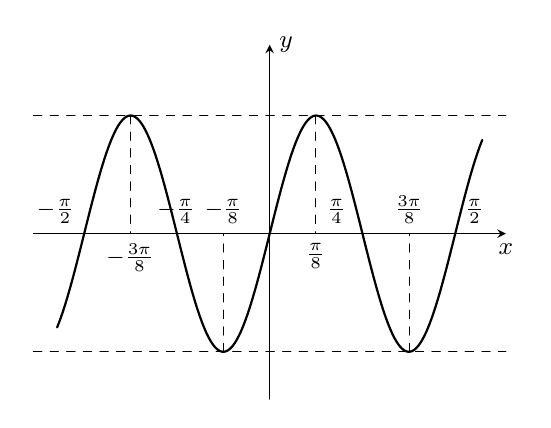
\begin{tikzpicture}[scale=1.5, font=\footnotesize, line join=round, line cap=round, >=stealth]
			\draw[->] (-2,0) -- (2,0) node[below] {\small $x$};
			\draw[->] (0,-1.4)-- (0,1.6) node[right] {\small $y$};
			\draw[thick,samples=300,domain=-1.8:1.8] plot(\x,{sin((4*\x)*180/pi)});
			\draw[dashed] (0.39,1)--(0.39,0) node[below] {$\frac{\pi}{8}$};
			\draw[dashed] (-0.39,-1)--(-0.39,0) node[above] {$-\frac{\pi}{8}$};
			\draw (-0.55,0) node[above left] {$-\frac{\pi}{4}$};	
			\draw (0.4,0) node[above right] {$\frac{\pi}{4}$};	
			\draw (-1.57,0) node[above left] {$-\frac{\pi}{2}$};
			\draw (1.57,0) node[above right] {$\frac{\pi}{2}$};	
			\draw[dashed] (-1.18,1)--(-1.18,0) node[below] {$-\frac{3\pi}{8}$};
			\draw[dashed] (1.18,-1)--(1.18,0) node[above] {$\frac{3\pi}{8}$};	
			\draw[dashed] (-2,1)--(2,1);
			\draw[dashed] (-2,-1)--(2,-1);
		\end{tikzpicture}	
	\end{center}
\end{bt}

\begin{bt}%[1D1H4-7]
% nguon: Archive/SP_KhoLatex/ID6_old/1K1-3.tex #3550
%[Dự án 1 - TLDH - TeamTeXHoa - Trần Trọng Tiên]
	Vẽ đồ thị hàm số $y=\cos\dfrac{x}{3}$.
	\loigiai{
		Miền xác định: $\mathscr{D}=\mathbb{R}$.\\
		Ta chỉ cần vẽ đồ thị hàm số trên miền $\left[0 ; 6\pi\right]$ (do chu kì tuần hoàn $T=2\pi:\dfrac{1}{3}=6\pi$).\\
		Bảng giá trị của hàm số $y=\cos\dfrac{x}{3}$ trên đoạn $\left[0 ; 6\pi\right]$ là
		\begin{center}
			\setlength\extrarowheight{10pt}
			\begin{tabular}{|c|c|c|c|c|c|c|c|c|c|}
				\hline
				$x$	& $0$ &$\dfrac{3\pi}{4}$  & $\dfrac{3\pi}{2}$ & $\dfrac{21\pi}{6}$ & $3\pi$  & $\dfrac{15\pi}{4}$ & $\dfrac{9\pi}{2}$ &$\dfrac{33\pi}{6}$  & $6\pi$ \\
				\hline
				$y$	& $1$  & $\dfrac{\sqrt{2}}{2}$ & $0$ & $-\dfrac{\sqrt{3}}{2}$ & $-1$ & $-\dfrac{\sqrt{2}}{2}$  & $0$ & $\dfrac{\sqrt{3}}{2}$ & $1$ \\
				\hline
			\end{tabular}
		\end{center}
		Ta có đồ thị của hàm số $y=\cos\dfrac{x}{3}$ trên đoạn  $\left[0 ; 6\pi\right]$ và sau đó tịnh tiến cho các đoạn: $\ldots,\left[-6\pi ; 0\right],\left[6\pi; 12\pi\right],\ldots$
	}
	\begin{center}
		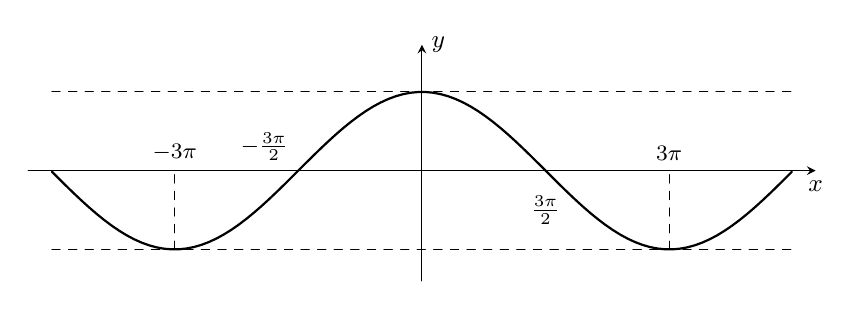
\begin{tikzpicture}[scale=1, font=\footnotesize, line join=round, line cap=round, >=stealth]
			\draw[->] (-5,0) -- (5,0) node[below] {\small $x$};
			\draw[->] (0,-1.4)-- (0,1.6) node[right] {\small $y$};
			\draw[thick,samples=100,domain=-4.7:4.7] plot(\x,{cos((\x)*180/pi)});
			\draw[dashed] (-3.14,-1)--(-3.14,0) node[above] {$-3\pi$};
			\draw[dashed] (3.14,-1)--(3.14,0) node[above] {$3\pi$};
			\draw (-1.57,0) node[above left] {$-\frac{3\pi}{2}$};
			\draw (1.57,-0.2) node[below] {$\frac{3\pi}{2}$};
			\draw[dashed] (-4.7,1)--(4.7,1);
			\draw[dashed] (-4.7,-1)--(4.7,-1);
			
		\end{tikzpicture}
	\end{center}
\end{bt}

\begin{bt}%[1D1H4-7]
% nguon: Archive/SP_KhoLatex/ID6_old/1K1-3.tex #3551
%[Dự án 1 - TLDH - TeamTeXHoa - Trần Trọng Tiên - Trần Trọng Tiên]
	Cho đồ thị hàm số $y=\sin x$, $(C)$. Hãy vẽ các đồ thị của các hàm số sau:
	\begin{listEX}[2]
		\item $y=\sin\left(x+\dfrac{\pi}{4}\right)$;
		\item $y=\sin \left(x+\dfrac{\pi}{4}\right)+2$.
	\end{listEX}
	\loigiai{
		Từ đồ thị hàm số $y=\sin x$, $(C)$ như sau:
		\begin{center}
			\begin{tikzpicture}[scale=1, font=\footnotesize, line join=round, line cap=round, >=stealth]
				\draw[->] (-4.7,0) -- (4.7,0) node[below] {\small $x$};
				\draw[->] (0,-1.4)node[below]{Đồ thị hàm số $y=\sin x$} -- (0,1.6) node[right] {\small $y$};
				\draw[thick,samples=100,domain=-4.7:4.7] plot(\x,{sin((\x)*180/pi)});
				\draw (-3.17,0) node[below] {$-\pi$};
				\draw (3.14,0) node[below] {$\pi$};
				\draw[dashed] (-1.57,-1)--(-1.57,0) node[above] {$-\frac{\pi}{2}$};
				\draw[dashed] (1.57,1)--(1.57,-0.2) node[below] {$\frac{\pi}{2}$};
				\draw[dashed] (-5,1)--(5,1);
				\draw[dashed] (-5,-1)--(5,-1);
			\end{tikzpicture}
		\end{center}
		\begin{listEX}[1]
			\item Từ đồ thị $(C)$, ta có đồ thị $y=\sin\left(x+\dfrac{\pi}{4}\right)$ bằng cách tịnh tiến $(C)$ sang trái một đoạn là $\dfrac{\pi}{4}$ đơn vị, ta được đồ thị hàm số $y=\sin\left(x+\dfrac{\pi}{4}\right)$, $(C')$ như hình vẽ dưới
			\begin{center}
				\begin{tikzpicture}[scale=1, font=\footnotesize, line join=round, line cap=round, >=stealth]
					\draw[->] (-4.7,0) -- (4.7,0) node[below] {\small $x$};
					\draw[->] (0,-1.4)node[below]{Đồ thị hàm số $y=\sin\left(x+\dfrac{\pi}{4}\right)$} -- (0,1.6) node[right] {\small $y$};
					\draw[thick,samples=100,domain=-4.7:4.7] plot(\x,{sin((\x+pi/4)*180/pi)});
					\draw (-3.8,0) node[above] {$\frac{-5\pi}{2}$};
					\draw (2.5,0) node[above] {$\frac{3\pi}{4}$};
					\draw (-0.79,0) node[above] {$\frac{-\pi}{4}$};
					\draw[dashed] (-2.36,-1)--(-2.36,0) node[above] {$-\frac{3\pi}{4}$};
					\draw[dashed] (0.79,1)--(0.79,-0.2) node[below] {$\frac{\pi}{4}$};
					\draw[dashed] (-5,1)--(5,1);
					\draw[dashed] (-5,-1)--(5,-1);
				\end{tikzpicture}
			\end{center}
			\item Từ đồ thị $(C")$, ta có đồ thị $y=\sin\left(x+\dfrac{\pi}{4}\right)+2$ bằng cách tịnh tiến $(C')$ lên trên một đoạn là $2$ đơn vị, ta được đồ thị hàm số $y=\sin\left(x+\dfrac{\pi}{4}\right)+2$, $(C'')$ như hình vẽ dưới
			\begin{center}
				\begin{tikzpicture}[scale=1, font=\footnotesize, line join=round, line cap=round, >=stealth]
					\draw[->] (-4.7,0) -- (4.7,0) node[below] {\small $x$};
					\draw[->] (0,-0.4)node[below]{Đồ thị hàm số $y=\sin\left(x+\dfrac{\pi}{4}\right)+2$} -- (0,3.6) node[right] {\small $y$};
					\draw[thick,samples=100,domain=-4.7:4.7] plot(\x,{sin((\x+pi/4)*180/pi)+2});
					\draw (-0.79,0) node[above] {$\frac{-\pi}{4}$};
					\draw (0.79,0) node[above right] {$\frac{\pi}{4}$};
					\draw[dashed] (-2.36,1)--(-2.36,0) node[above right] {$-\frac{3\pi}{4}$};
					\draw[dashed] (3.93,1)--(3.93,0) node[above right] {$\frac{5\pi}{4}$};
					\draw[dashed] (0.79,0)--(0.79,3);
					\draw[dashed] (-5,1)--(5,1);
					\draw[dashed] (-5,3)--(5,3);
				\end{tikzpicture}
			\end{center}
		\end{listEX}
	}
\end{bt}

\begin{bt}%[1D1H4-2]
% nguon: Archive/SP_KhoLatex/ID6_old/1K1-3.tex #3552
%[Dự án 1 - TLDH - TeamTeXHoa - Trần Trọng Tiên]
	Tìm tập xác định của các hàm số sau:
	\begin{listEX}[2]
		\item $y=\dfrac{1-\cos x}{\sin x}$;
		\item $y=\sqrt{\dfrac{1+\cos x}{2-\cos x}}$.
	\end{listEX}
	\loigiai{
		\begin{listEX}[1]
			\item Biểu thức $y=\dfrac{1-\cos x}{\sin x}$ có nghĩa khi $\sin x\ne 0$, tức là $x\ne k\pi,~k\in\mathbb{Z}$.\\
			Vậy tập xác định của hàm số $y=\dfrac{1-\cos x}{\sin x}$ là $\mathscr{D}=\mathbb{R}\setminus k\pi,~k\in\mathbb{Z}$.
			\item Biểu thức $y=\sqrt{\dfrac{1+\cos x}{2-\cos x}}$ có nghĩa khi $\heva{&\sqrt{\dfrac{1+\cos x}{2-\cos x}}\ge 0\\&2-\cos x\ne 0.}$\\
			Vì $-1\le \cos x\le 1$ nên $1+\cos x\ge 0$ với mọi $x\in \mathbb{R}$ và $\sqrt{\dfrac{1+\cos x}{2-\cos x}}\ge 0$ với mọi $x\in \mathbb{R}$.\\
			Vậy tập xác định của hàm số $y=\sqrt{\dfrac{1+\cos x}{2-\cos x}}$ là $\mathscr{D}=\mathbb{R}$.
		\end{listEX}
	}
\end{bt}

\begin{bt}%[1D1H4-4]
% nguon: Archive/SP_KhoLatex/ID6_old/1K1-3.tex #3553
%[Dự án 1 - TLDH - TeamTeXHoa - Trần Trọng Tiên]
	Xét tính chẵn lẻ của các hàm số sau:
	\begin{listEX}[2]
		\item $y=\sin 2x+\tan 2x$;
		\item $y=\cos x+\sin^2x$;
		\item $y=\sin x\cos 2x$;
		\item $y=\sin x+\cos x$.
	\end{listEX}
	\loigiai{
		\begin{listEX}[1]
			\item Biểu thức $\sin 2x+\tan 2x$ có nghĩa khi $\cos 2x\ne 0$ $\left(\text{do } \tan 2x=\dfrac{\sin 2x}{\cos 2x}\right)$, tức là 
			\[2x\ne \dfrac{\pi}{2}+k\pi,~k\in\mathbb{Z}\Leftrightarrow x\ne\dfrac{\pi}{4}+k\dfrac{\pi}{2},~k\in\mathbb{Z}.\]
			Suy ra tập xác định của hàm số $y=f(x)=\sin 2x+\tan 2x$ là $\mathscr{D}=\mathbb{R}\setminus \left\{\dfrac{\pi}{4}+k\dfrac{\pi}{2}\big |k\in\mathbb{R}\right\}$.\\
			Do đó, nếu $x$ thuộc tập xác định $\mathscr{D}$ thì $-x$  cũng thuộc tập xác định $\mathscr{D}$. Ta có\\
			$f(-x)=\sin(-2x)+\tan(-2x)=-\sin 2x-\tan 2x=-(\sin 2x+\tan 2x)=-f(x)$, với mọi $x$ thuộc $\mathscr{D}$.\\
			Vậy $y=\sin 2x+\tan 2x$ là hàm số lẻ.
			\item Tập xác định của hàm số $y=\cos x+\sin^2x$ là $\mathscr{D}=\mathbb{R}$.\\
			Do đó, nếu $x$ thuộc tập xác định $\mathscr{D}$ thì $-x$ cũng thuộc tập xác định $\mathscr{D}$.\\
			Ta có $f(-x)=\cos(-x)+\sin^2(-x)=\cos x+(\sin x)^2=\cos x+\sin^2x=f(x),~\forall x\in\mathscr{D}$.\\
			Vậy $y=\cos x+\sin^2 x$ là hàm số chẵn.	
			\item Tập xác định của hàm số $y=\sin x\cos 2x$ là $\mathscr{D}=\mathbb{R}$.\\
			Do đó, nếu $x$ thuộc tập xác định $\mathscr{D}$ thì $-x$ cũng thuộc tập xác định $\mathscr{D}$.\\
			Ta có $f(-x)=\sin (-x)\cdot\cos (-2x)=-\sin x\cdot\cos 2x= -f(x),~\forall x\in\mathscr{D}$.\\
			Vậy $y=\sin x\cos 2x$  là hàm số lẻ.
			\item Tập xác định của hàm số $y=\sin x+\cos x$ là $\mathscr{D}=\mathbb{R}$.\\
			Do đó, nếu $x$ thuộc tập xác định $\mathscr{D}$ thì $-x$ cũng thuộc tập xác định $\mathscr{D}$.\\
			Ta có $f(-x)=\sin (-x)+\cos (-x)=-\sin x+\cos x\ne-f(x)$.\\
			Vậy $y=\sin x+\cos x$  là hàm số không chẵn, không lẻ.
		\end{listEX}
	}
\end{bt}

\begin{bt}%[1D1H1-5]
% nguon: Archive/SP_KhoLatex/ID6_old/1K1-1-4.tex #3556

	Biểu diễn trên đường tròn lượng giác các góc lượng giác có số đo sau:
	\begin{enumEX}{2}
		\item $750^{\circ}$;
		\item $-1125^{\circ}$.
	\end{enumEX}
\loigiai{
	\begin{enumerate}
		\item Ta có $750^{\circ}=30^{\circ}+2\cdot360^{\circ}$. Vậy điểm biểu diễn góc lượng giác có số đo $750^{\circ}$ là điểm $M$ trên phần đường tròn lượng giác thuộc góc phần tư thứ I sao cho $\widehat{A O M}=30^{\circ}$. 
		\begin{center}
			\begin{tikzpicture}[scale=.8,>=stealth, font=\footnotesize, line join=round, line cap=round]
				\draw[fill=black](0,0) coordinate (O) node[below left]{$O$} circle (1.5pt) (2,0) coordinate (A) node[above right] {$A$} circle (1.5pt) (30:2) coordinate (M) node [right] {$M$} circle (1.5 pt);
				\draw[very thick] (0,0) circle (2 cm);
				\draw[->] (-3,0)--(3,0) node [below]{$x$};
				\draw[->] (0,-3)--(0,3) node [left]{$y$};
				\clip (-5,-5) rectangle (5,5);
				\draw (3,3) node {I} (-3,3) node {II} (-3,-3) node {III} (3,-3) node {IV};
				\draw (M)--(O);
				\pic [draw, ->, "$\alpha$", angle eccentricity=1.5] {angle = A--O--M};
			\end{tikzpicture}
		\end{center}
		\item Ta có $-1125^{\circ}=-45^{\circ}-3\cdot360^{\circ}$. Vậy điểm biểu diễn góc lượng giác có số đo $-1125^{\circ}$ là điểm $M$ trên phần đường tròn lượng giác thuộc góc phần tư thứ IV sao cho $\widehat{A O M}=45^{\circ}$. 
		\begin{center}
			\begin{tikzpicture}[scale=.8,>=stealth, font=\footnotesize, line join=round, line cap=round]
				\draw[fill=black](0,0) coordinate (O) node[below left]{$O$} circle (1.5pt) (2,0) coordinate (A) node[above right] {$A$} circle (1.5pt) (-45:2) coordinate (M) node [below right] {$M$} circle (1.5 pt);
				\draw[very thick] (0,0) circle (2 cm);
				\draw[->] (-3,0)--(3,0) node [below]{$x$};
				\draw[->] (0,-3)--(0,3) node [left]{$y$};
				\clip (-5,-5) rectangle (5,5);
				\draw (3,3) node {I} (-3,3) node {II} (-3,-3) node {III} (3,-3) node {IV};
				\draw (M)--(O);
				\pic [draw, <-, "$\alpha$", angle eccentricity=1.5] {angle = M--O--A};
			\end{tikzpicture}
		\end{center}
	\end{enumerate}
}
\end{bt}

\begin{bt}%[1D1H1-5]
% nguon: Archive/SP_KhoLatex/ID6_old/1K1-1-4.tex #3557

	Biểu diễn trên đường tròn lượng giác các góc lượng giác có số đo sau:
	\begin{enumEX}{2}
		\item $\dfrac{9\pi}{2}$;
		\item $-\dfrac{37\pi}{6}$.
	\end{enumEX}
\loigiai{
	\begin{enumerate}
	\item Ta có $\dfrac{9\pi}{2}=\dfrac{\pi}{2}+2\cdot2\pi$. Vậy điểm biểu diễn góc lượng giác có số đo $\dfrac{9\pi}{2}$ là điểm $M$ trên phần đường tròn lượng giác sao cho $\widehat{A O M}=\dfrac{\pi}{2}$. 
	\begin{center}
		\begin{tikzpicture}[scale=.8,>=stealth, font=\footnotesize, line join=round, line cap=round]
			\draw[fill=black](0,0) coordinate (O) node[below left]{$O$} circle (1.5pt) (2,0) coordinate (A) node[above right] {$A$} circle (1.5pt) (90:2) coordinate (M) node [above right] {$M$} circle (1.5 pt);
			\draw[very thick] (0,0) circle (2 cm);
			\draw[->] (-3,0)--(3,0) node [below]{$x$};
			\draw[->] (0,-3)--(0,3) node [left]{$y$};
			\clip (-5,-5) rectangle (5,5);
			\draw (3,3) node {I} (-3,3) node {II} (-3,-3) node {III} (3,-3) node {IV};
			\draw (M)--(O);
			\pic [draw, ->, "$\alpha$", angle eccentricity=1.5] {angle = A--O--M};
		\end{tikzpicture}
	\end{center}
	\item Ta có $-\dfrac{37\pi}{6}=-\dfrac{\pi}{6}-3\cdot2\pi$. Vậy điểm biểu diễn góc lượng giác có số đo $-\dfrac{37\pi}{6}$ là điểm $M$ trên phần đường tròn lượng giác thuộc góc phần tư thứ IV sao cho $\widehat{A O M}=\dfrac{\pi}{6}$. 
	\begin{center}
		\begin{tikzpicture}[scale=.8,>=stealth, font=\footnotesize, line join=round, line cap=round]
			\draw[fill=black](0,0) coordinate (O) node[below left]{$O$} circle (1.5pt) (2,0) coordinate (A) node[above right] {$A$} circle (1.5pt) (-30:2) coordinate (M) node [below right] {$M$} circle (1.5 pt);
			\draw[very thick] (0,0) circle (2 cm);
			\draw[->] (-3,0)--(3,0) node [below]{$x$};
			\draw[->] (0,-3)--(0,3) node [left]{$y$};
			\clip (-5,-5) rectangle (5,5);
			\draw (3,3) node {I} (-3,3) node {II} (-3,-3) node {III} (3,-3) node {IV};
			\draw (M)--(O);
			\pic [draw, <-, "$\alpha$", angle eccentricity=1.5] {angle = M--O--A};
		\end{tikzpicture}
	\end{center}
	\end{enumerate}
}
\end{bt}

\begin{bt}%[1D1V1-5]
% nguon: Archive/SP_KhoLatex/ID6_old/1K1-1-4.tex #3558

	Biểu diễn trên đường tròn lượng giác các góc lượng giác có số đo sau:
	\begin{enumEX}{2}
		\item $\dfrac{\pi}{6}+k\pi$;
		\item $-\dfrac{\pi}{4}+\dfrac{k2\pi}{3}$.
	\end{enumEX}
	\loigiai{
\immini{
	\begin{enumerate}
		\item Ta có $\alpha=\dfrac{\pi}{6}+k\pi=\dfrac{\pi}{6}+\dfrac{k2\pi}{2}$ do đó có hai điểm biểu diễn góc  $\alpha$ lần lượt là $\dfrac{\pi}{6}$ biểu diễn bởi $A_1$ và $\dfrac{7\pi}{6}$ biểu diễn $A_2$.
		\item Ta có $\alpha=\dfrac{\pi}{4}+\dfrac{k2\pi}{3}$ có ba điểm biểu diễn góc $\alpha$ lần lượt là $\dfrac{\pi}{4}$ biểu diễn bởi $B_1$, $\dfrac{11\pi}{12}$ biểu diễn bởi $B_2$ và $\dfrac{19\pi}{12}$ biểu diễn bởi $B_3$.
	\end{enumerate}
}{
	\begin{tikzpicture}[scale=.8,>=stealth, font=\footnotesize, line join=round, line cap=round]
		\draw[fill=black](0,0) coordinate (O) node[below left]{$O$} circle (1.5pt) (30:2) coordinate (A1) node[right] {$A_1$} circle (1.5pt) (210:2) coordinate (A2) node [below left] {$A_2$} circle (1.5 pt) (45:2) coordinate (B1) node [above right] {$B_1$} circle (1.5pt) (165:2) coordinate (B2) node [above left] {$B_2$} circle (1.5pt) (285:2) coordinate (B3) node [below right] {$B_3$} circle (1.5pt);
		\draw[very thick] (0,0) circle (2 cm);
		\draw[->] (-3,0)--(3,0) node [below]{$x$};
		\draw[->] (0,-3)--(0,3) node [left]{$y$};
		\clip (-5,-5) rectangle (5,5);
	\end{tikzpicture}
}
}
\end{bt}

\begin{bt}%[1D1V1-5]
% nguon: Archive/SP_KhoLatex/ID6_old/1K1-1-4.tex #3559

	Khi biểu diễn các góc lượng giác có số đo $x=\dfrac{\pi}{2}+k \pi$ và $y=\dfrac{\pi}{2}+k 2 \pi$ lên đường tròn lượng giác, số điểm chung nhận được là bao nhiêu?
	\loigiai{
	Ta có $x=\dfrac{\pi}{2}+k \pi=\dfrac{\pi}{2}+\dfrac{k 2 \pi}{2}$. Vậy có 2 điểm biểu diễn góc lượng giác có số đo $x$.
	\begin{itemize}
	\item 	Với $k=0,\ x_1=\dfrac{\pi}{2}$, được biểu diễn bởi điểm $B$.
	\item 	Với $k=1,\ x_2=\dfrac{3 \pi}{2}$ được biểu diễn bởi điểm $B'$.
	\end{itemize}
	Ta có $y=\dfrac{\pi}{2}+k 2 \pi$. Vậy có 1 điểm biểu diễn góc lượng giác có số đo $y$. Với $k=0, y=\dfrac{\pi}{2}$, được biểu diễn bởi điểm $B$. Vậy số điểm chung nhận được là 1 điểm chung.
}
\end{bt}

\begin{bt}%[1D1C1-5]
% nguon: Archive/SP_KhoLatex/ID6_old/1K1-1-4.tex #3560

	Xác định công thức hợp nhất của hai góc lượng giác $x_1=k\pi$ và $x_2=\dfrac{\pi}{2}+k\pi$.
	\loigiai{
	Ta có $x_1=k\pi=\dfrac{k2\pi}{2}$ có hai điểm biểu diễn cho góc $x_1$ với $0$ biểu diễn bởi $A_1$ và $\pi$ biểu diễn bởi $A_2$.\\
	$x_2 = \dfrac{\pi}{2}+k\pi=\dfrac{\pi}{2}+\dfrac{k2\pi}{2}$ có hai điểm biểu diễn với $\dfrac{\pi}{2}$ biểu diễn bởi $B_1$ và $\dfrac{3\pi}{2}$ biểu diễn bởi $B_2$.\\
	Dễ thấy 4 điểm này cách đều nhau do đó có thể gộp hai hai góc lượng giác này lại thành công thức duy nhất là $\dfrac{k2\pi}{4}=\dfrac{k\pi}{2}$. 
}
\end{bt}

\begin{bt}%[1D1H2-2]
% nguon: Archive/SP_KhoLatex/ID6_old/1K1-1-5.tex #3565

	Xét dấu các giá trị lượng giác của góc lượng giác $\alpha=\dfrac{5 \pi}{6}$.
	\loigiai{
		Do $\dfrac{\pi}{2}<\dfrac{5 \pi}{6}<\pi$ nên $\sin \left(\dfrac{5 \pi}{6}\right)>0; \cos \left(\dfrac{5 \pi}{6}\right)<0; \tan \left(\dfrac{5 \pi}{6}\right)<0; \cot \left(\dfrac{5 \pi}{6}\right)<0$.
	}
\end{bt}

\begin{bt}%[1D1V2-2]
% nguon: Archive/SP_KhoLatex/ID6_old/1K1-1-5.tex #3567

	Cho $0^{\circ}<\alpha<90^{\circ}$. Xét dấu các biểu thức sau:
	\begin{enumEX}{2}
		\item  $A=\cos \left(\alpha+90^{\circ}\right)$;
		\item  $B=\sin \left(\alpha+80^{\circ}\right)$.
	\end{enumEX}
	\loigiai{
		\begin{enumerate}
			\item $A=\cos \left(\alpha+90^{\circ}\right)=\cos \left(90^{\circ}-(-\alpha)\right)=\sin(-\alpha)=-\sin \alpha$.\\
			Vì $0^{\circ}<\alpha<90^{\circ}$ nên $\sin \alpha>0$.\\
			Do đó $A<0$.
			\item $B=\sin \left(\alpha+80^{\circ}\right)$.\\
			Vì $0^{\circ}<\alpha<90^{\circ}$ nên $80^{\circ}<\alpha+80^{\circ}<170^{\circ}$.\\
			Do đó, điểm cuối của cung $\alpha+80^{\circ}$ thuộc góc phần tư thứ I hoặc thứ II nên $B>0$.
		\end{enumerate}
	}
	
\end{bt}

\begin{bt}%[1D1H3-2]
% nguon: Archive/SP_KhoLatex/ID6_old/1K1-2.tex #3577
%[Dự án 1 - TLDH - TeamTeXHoa - DiaMond]
Biết $\sin x=\dfrac{1}{2}$, $0<x<\dfrac{\pi }{2}$. Hãy tính giá trị lượng giác $\cos\left(x+\dfrac{\pi}{4}\right)$.
\loigiai{
Vì $0<x<\dfrac{\pi}{2}$ nên điểm ngọn cung thuộc góc phần tư thứ I $\Rightarrow \cos x>0\Rightarrow \cos x=\dfrac{\sqrt{3}}{2}$.\\
Ta có 
\begin{eqnarray*}
\cos\left(x+\dfrac{\pi}{4}\right)&=&\cos x\cdot\cos\dfrac{\pi}{4}-\sin x\cdot\sin \dfrac{\pi }{4}\\
&=&\dfrac{\sqrt{2}}{2}\cos x-\dfrac{\sqrt{2}}{2}\sin x\\
&=&\dfrac{\sqrt{2}}{2}\cdot\dfrac{\sqrt{3}}{2}-\dfrac{\sqrt{2}}{2}\cdot\dfrac{1}{2}\\
&=&\dfrac{\sqrt{6}-\sqrt{2}}{4}.
\end{eqnarray*}
}
\end{bt}

\begin{bt}%[1D1H3-2]
% nguon: Archive/SP_KhoLatex/ID6_old/1K1-2.tex #3578
%[Dự án 1 - TLDH - TeamTeXHoa - DiaMond]
Biết $\cos x=-\dfrac{12}{13}$, $\pi <x<\dfrac{3\pi}{2}$. Tính giá trị lượng giác $\sin\left(\dfrac{\pi}{3}-x\right)$.
\loigiai{
Vì $\pi <x<\dfrac{3\pi }{2}$ nên điểm ngọn cung thuộc góc phần tư thứ III.\\
Suy ra $\sin x<0\Rightarrow \sin x=-\sqrt{1-\cos^2x}=-\sqrt{1-\left( \dfrac{-12}{13}\right)^2}=-\dfrac{5}{13}$.\\
Ta có $\sin\left(\dfrac{\pi }{3}-x\right)=\sin\dfrac{\pi }{3}\cos x-\cos \dfrac{\pi }{3}\sin x=\dfrac{\sqrt{3}}{2}\cdot\dfrac{-12}{13}-\dfrac{1}{2}\cdot\dfrac{-5}{13}=\dfrac{5-12\sqrt{3}}{26}$.
}
\end{bt}

\begin{bt}%[1D1V3-2]
% nguon: Archive/SP_KhoLatex/ID6_old/1K1-2.tex #3579
%[Dự án 1 - TLDH - TeamTeXHoa - DiaMond]
Rút gọn biểu thức $A=\sin(x+14^\circ)\sin(x+74^\circ)+\sin(x-76^\circ)\sin(x-16^\circ)$. 
\loigiai{
Ta có
\begin{eqnarray*}
A&=&\sin(14^\circ+x)\cos(16^\circ-x)+\sin(76^\circ-x)\sin(16^\circ-x)\\
&=&\sin(14^\circ+x)\cos(16^\circ-x)+\cos(14^\circ+x)\sin(16^\circ-x)\\
&=&\sin(14^\circ+16^\circ+x-x)\\
&=&\sin30^\circ=\dfrac{1}{2}.
\end{eqnarray*}
}
\end{bt}

\begin{bt}%[1D1V3-2]
% nguon: Archive/SP_KhoLatex/ID6_old/1K1-2.tex #3580
%[Dự án 1 - TLDH - TeamTeXHoa - DiaMond]
Rút gọn biểu thức $A=\dfrac{\sin ( a-b )}{\cos a\cos b}+\dfrac{\sin ( b-c )}{\cos b\cos c}+\dfrac{\sin ( c-a )}{\cos c\cos a}$. 
\loigiai{
Ta có
\begin{eqnarray*}
A&=&\dfrac{\sin a\cdot\cos b-\sin b\cdot\cos a}{\cos a\cdot\cos b}+\dfrac{\sin b\cdot\cos c-\sin c\cdot\cos b}{\cos b\cdot\cos c}+\dfrac{\sin c\cdot\cos a-\sin a\cdot\cos c}{\cos c\cdot\cos a}\\
&=&\dfrac{\sin a\cdot\cos b}{\cos a\cdot\cos b}-\dfrac{\sin b\cdot\cos a}{\cos a\cdot\cos b}+\dfrac{\sin b\cdot\cos c}{\cos b\cdot\cos c}-\dfrac{\sin c\cdot\cos b}{\cos b\cdot\cos c}+\dfrac{\sin c\cdot\cos a}{\cos c\cdot\cos a}-\dfrac{\sin a\cdot\cos c}{\cos c\cdot\cos a}\\ 
&=&\tan a-\tan b+\tan b-\tan c+\tan c-\tan a\\
&=&0.
\end{eqnarray*}
}
\end{bt}

\begin{bt}%[1D1V3-2]
% nguon: Archive/SP_KhoLatex/ID6_old/1K1-2.tex #3581
%[Dự án 1 - TLDH - TeamTeXHoa - DiaMond]
Không dùng MTCT, tính các giá trị lượng giác sau $\cos 795^\circ$, $\tan \dfrac{7\pi }{12}$. 
\loigiai{
\begin{enumerate}
\item Tính $\cos 795^\circ$.\\
Vì $795^\circ=75^\circ+2\cdot 360^\circ=30^\circ+45^\circ+2\cdot360^\circ$ nên
\begin{eqnarray*}
\cos 795^\circ&=&\cos 75^\circ\\
&=&\cos 30^\circ\cos 45^\circ-\sin 30^\circ\sin 45^\circ\\
&=&\dfrac{\sqrt{3}}{2}\cdot\dfrac{\sqrt{2}}{2}-\dfrac{1}{2}\cdot\dfrac{\sqrt{2}}{2}\\
&=&\dfrac{\sqrt{6}-\sqrt{2}}{4}.
\end{eqnarray*}
\item Ta có $\tan \dfrac{7\pi }{12}=\tan ( \dfrac{\pi }{3}+\dfrac{\pi }{4} )=\dfrac{\tan \dfrac{\pi }{3}+\tan \dfrac{\pi }{4}}{1-\tan \dfrac{\pi }{3}\tan \dfrac{\pi }{4}}=\dfrac{\sqrt{3}+1}{1-\sqrt{3}}=-2-\sqrt{3}$.
\end{enumerate}
}
\end{bt}

\begin{bt}%[1D1V3-5]
% nguon: Archive/SP_KhoLatex/ID6_old/1K1-2.tex #3582
%[Dự án 1 - TLDH - TeamTeXHoa - DiaMond]
Tính giá trị biểu thức lượng giác sau
\begin{enumerate}
\item $A=\sin 22^\circ30'\cos 202^\circ30'$.
\item $B=4\sin^4\dfrac{\pi}{16}+2\cos\dfrac{\pi}{8}$.
\end{enumerate}
\loigiai{
\begin{enumerate}
\item $A=\sin 22^\circ30'\cos 202^\circ30'$.\\
\textbf{Cách 1.} Ta có $\cos 202^\circ30'=\cos (180^\circ+22^\circ30')=-\cos 22^\circ30'$.\\
Do đó $A=-\sin 22^\circ30'\cos 22^\circ30'=-\dfrac{1}{2}\sin 45^\circ=-\dfrac{\sqrt{2}}{4}$.\\
\textbf{Cách 2.} Ta có
\begin{eqnarray*}
A&=&\dfrac{1}{2}[\sin(22^\circ30'+202^\circ30')+\sin (22^\circ30'-202^\circ30')]\\
&=&\dfrac{1}{2}[\sin 225^\circ+\sin (-180^\circ)]=\dfrac{1}{2}[\sin (180^\circ+45^\circ)-\sin 180^\circ]\\
&=&-\dfrac{1}{2}\sin 45^\circ=-\dfrac{\sqrt{2}}{4}.
\end{eqnarray*}
\item Ta có
\begin{eqnarray*}
B&=&\left(2\sin^2\dfrac{\pi}{16}\right)^2+2\cos\dfrac{\pi}{8}\\
&=&\left[1-\cos\left(2\cdot\dfrac{\pi }{16}\right)\right]^2+2\cos \dfrac{\pi }{8}\\
&=&1-2\cos \dfrac{\pi}{8}+{\cos^2}\dfrac{\pi}{8}+2\cos\dfrac{\pi}{8}\\
&=&1+\dfrac{1+\cos \dfrac{\pi }{4}}{2}\\
&=&1+\dfrac{1+\dfrac{\sqrt{2}}{2}}{2}\\
&=&\dfrac{6+\sqrt{2}}{4}.
\end{eqnarray*}
\end{enumerate}
}
\end{bt}

\begin{bt}%[1D1V3-2]
% nguon: Archive/SP_KhoLatex/ID6_old/1K1-2.tex #3583
%[Dự án 1 - TLDH - TeamTeXHoa - DiaMond]
Tính giá trị biểu thức lượng giác sau
\begin{enumerate}
\item $A=\dfrac{1}{\cos290^\circ}+\dfrac{1}{\sqrt{3}{\sin250^\circ}}$.
\item $B=(1+\tan20^\circ)( 1+\tan25^\circ)$.
\item $C=\tan 9^\circ-\tan 27^\circ-\tan 63^\circ+\tan 81^\circ$.
\item $D=\sin ^2\dfrac{\pi }{9}+\sin ^2\dfrac{2\pi }{9}+\sin \dfrac{\pi }{9}\sin \dfrac{2\pi }{9}$.
\end{enumerate}
\loigiai{
\begin{enumerate}
\item Ta có $\cos 290^\circ=\cos (180^\circ+90^\circ+20^\circ)=-\cos(90^\circ+20^\circ)=\sin 20^\circ$ \\
và $\sin 250^\circ=\sin (180^\circ+90^\circ-20^\circ)=-\sin (90^\circ-20^\circ)=-\cos 20^\circ$.\\
Suy ra 
\begin{eqnarray*}
A&=&\dfrac{1}{\sin20^\circ}-\dfrac{1}{\sqrt{3}{\cos 20^\circ}}\\
&=&\dfrac{\sqrt{3}\cos20^\circ-\sin20^\circ}{\sqrt{3}\sin20^\circ\cos20^\circ}\\
&=&4\cdot\dfrac{\dfrac{\sqrt{3}}{2}\cos 20^\circ-\dfrac{1}{2}\sin 20^\circ}{\sqrt{3}\cdot 2\cdot \sin 20^\circ\cdot\cos 20^\circ}\\
&=&4\dfrac{\sin 60^\circ\cos 20^\circ-\cos 60^\circ\sin 20^\circ}{\sqrt{3}\sin 40^\circ}\\
&=&\dfrac{4\sin {{40}^\circ}}{\sqrt{3}\sin {{40}^\circ}}\\
&=&\dfrac{4\sqrt{3}}{3}.
\end{eqnarray*}
\item \textbf{Cách 1.} Ta có 
\begin{eqnarray*}
B&=&\left(1+\dfrac{\sin 20^\circ}{\cos 20^\circ}\right)\left(1+\dfrac{\sin 25^\circ}{\cos 25^\circ}\right)\\
&=&\dfrac{\sin20^\circ+\cos20^\circ}{\cos20^\circ}\cdot\dfrac{\sin25^\circ+\cos25^\circ}{\cos25^\circ}\\
&=&\sqrt{2}\cdot\dfrac{\sin20^\circ\cos45^\circ+\cos20^\circ\sin45^\circ}{\cos20^\circ}\cdot\sqrt{2}\cdot\dfrac{\sin25^\circ\cos45^\circ+\cos25^\circ\sin45^\circ}{\cos25^\circ}\\
&=&2\dfrac{\sin65^\circ\sin70^\circ}{\cos20^\circ\cos25^\circ}\\
&=&2.
\end{eqnarray*}
\textbf{Cách 2.} Ta có $\tan 45^\circ=\tan(20^\circ+50^\circ)=\dfrac{\tan20^\circ+\tan25^\circ}{1-\tan20^\circ\tan25^\circ}$.\\
Suy ra
\begin{eqnarray*}
1=\dfrac{\tan20^\circ+\tan25^\circ}{1-\tan20^\circ\tan25^\circ}&\Leftrightarrow& \tan20^\circ+\tan25^\circ+\tan20^\circ\tan25^\circ=1\\
&\Leftrightarrow& (1+\tan20^\circ)(1+\tan25^\circ)=2.
\end{eqnarray*}
Vậy $B=2$.
\item Ta có
\begin{eqnarray*}
C&=&\tan 9^\circ+\tan 81^\circ-(\tan 27^\circ+\tan 63^\circ )\\
&=&\dfrac{\sin 9^\circ\cos 81^\circ+\sin 81^\circ\cos 9^\circ}{\cos 9^\circ\cos 81^\circ}-\dfrac{\sin 27^\circ\cos 63^\circ+\sin 63^\circ\cos 27^\circ}{\cos 27^\circ\cos 63^\circ}\\
&=&\dfrac{1}{\cos 9^\circ\sin 9^\circ}-\dfrac{1}{\cos 27^\circ\sin 27^\circ}\\
&=&\dfrac{2}{\sin 18^\circ}-\dfrac{2}{\sin 54^\circ}\\
&=&\dfrac{2( \sin 54^\circ-\sin 18^\circ)}{\sin 18^\circ\sin 54^\circ}\\
&=&\dfrac{4\cos 36^\circ\sin 18^\circ}{\sin 18^\circ\sin 54^\circ}\\
&=&4.
\end{eqnarray*}
\item Ta có
\begin{eqnarray*}
D&=&\sin ^2\dfrac{\pi }{9}+\sin ^2\dfrac{2\pi }{9}+\sin \dfrac{\pi }{9}\sin \dfrac{2\pi }{9}\\
&=&\left(\sin\dfrac{\pi}{9}+\sin\dfrac{2\pi}{9}\right)^2-\sin \dfrac{\pi }{9}\sin \dfrac{2\pi }{9}\\
&=&\left(2\sin \dfrac{\pi }{6}\cos \dfrac{\pi }{18}\right)^2+\dfrac{1}{2}\left(\cos \dfrac{\pi }{3}-\cos \dfrac{\pi }{9} \right)\\
&=&\cos ^2\dfrac{\pi }{18}+\dfrac{1}{2}\left(\dfrac{1}{2}-\cos\dfrac{\pi}{9}\right)\\ 
&=&\dfrac{1+\cos \dfrac{\pi}{9}}{2}+\dfrac{1}{2}\left(\dfrac{1}{2}-\cos \dfrac{\pi }{9}\right)\\
&=&\dfrac{3}{4}.
\end{eqnarray*}
\end{enumerate}
}
\end{bt}

\begin{bt}%[1D1V3-3]
% nguon: Archive/SP_KhoLatex/ID6_old/1K1-2.tex #3584
%[Dự án 1 - TLDH - TeamTeXHoa - DiaMond]
Tính giá trị biểu thức lượng giác sau
\begin{enumerate}
\item $A=\sin \dfrac{\pi}{32}\cos \dfrac{\pi}{32}\cos \dfrac{\pi}{16}\cos \dfrac{\pi}{8}$.
\item $B=\sin 10^\circ\cdot\sin 30^\circ\cdot\sin 50^\circ\cdot\sin 70^\circ$.
\item $C=\cos\dfrac{\pi}{5}+\cos \dfrac{3\pi }{5}$.
\item $D=\cos^2\dfrac{\pi}{7}+\cos^2\dfrac{2\pi}{7}+\cos^2\dfrac{3\pi}{7}$.
\end{enumerate}
\loigiai{
\begin{enumerate}
\item Ta có
\begin{eqnarray*}
A&=&\dfrac{1}{2}\left(2\sin\dfrac{\pi}{32}\cos\dfrac{\pi}{32}\right)\cos \dfrac{\pi}{16}\cos\dfrac{\pi}{8}\\
&=&\dfrac{1}{2}\sin\dfrac{\pi}{16}\cos\dfrac{\pi}{16}\cos\dfrac{\pi}{8}\\
&=&\dfrac{1}{4}\sin\dfrac{\pi}{8}\cos\dfrac{\pi}{8}\\
&=&\dfrac{1}{8}\sin\dfrac{\pi}{4}\\
&=&\dfrac{\sqrt{2}}{16}.
\end{eqnarray*}
\item Ta có $B=\dfrac{1}{2}\cos20^\circ\cos40^\circ\cos80^\circ$ do đó 
\begin{eqnarray*}
16\sin20^\circ\cdot B&=&8\sin20^\circ\cos20^\circ\cos40^\circ\cos80^\circ\\
&=&4\sin40^\circ\cos40^\circ\cos80^\circ\\ 
&=&2\sin80^\circ\cos80^\circ\\
&=&\sin160^\circ.
\end{eqnarray*}
Suy ra $B=\dfrac{\sin160^\circ}{16\sin20^\circ}=\dfrac{1}{16}$.
\item Ta có $C=2\cos \dfrac{\pi }{5}\cos \dfrac{2\pi }{5}$. \\
Vì $\sin \dfrac{\pi }{5}\neq 0$ nên
$2\sin \dfrac{\pi }{5}\cdot C=4\sin \dfrac{\pi }{5}\cos \dfrac{\pi }{5}\cos \dfrac{2\pi }{5}=2\sin \dfrac{2\pi }{5}\cos \dfrac{2\pi }{5}=\sin \dfrac{4\pi }{5}$.\\
Suy ra $C=\dfrac{1}{2}$.
\item $D=\dfrac{1+\cos \dfrac{2\pi }{7}}{2}+\dfrac{1+\cos \dfrac{4\pi }{7}}{2}+\dfrac{1+\cos \dfrac{6\pi }{7}}{2}=\dfrac{3}{2}+\dfrac{1}{2}( \cos \dfrac{2\pi }{7}+\cos \dfrac{4\pi }{7}+\cos \dfrac{6\pi }{7} )$.\\
Xét $T=\cos \dfrac{2\pi }{7}+\cos \dfrac{4\pi }{7}+\cos \dfrac{6\pi }{7}$, vì $\sin \dfrac{\pi }{7}\ne 0$ nên
\begin{eqnarray*}
2\sin \dfrac{\pi }{7}T&=&2\sin \dfrac{\pi }{7}\cos \dfrac{2\pi }{7}+2\sin \dfrac{\pi }{7}\cos \dfrac{4\pi }{7}+2\sin \dfrac{\pi }{7}\cos \dfrac{6\pi }{7} \\ 
&=&( \sin \dfrac{3\pi }{7}-\sin \dfrac{\pi }{7} )+( \sin \dfrac{5\pi }{7}-\sin \dfrac{3\pi }{7} )+( \sin \pi -\sin \dfrac{5\pi }{7} ) \\ 
&=&-\sin \dfrac{\pi }{7}.
\end{eqnarray*}
Suy ra $T=-\dfrac{1}{2}$.\\
Vậy $D=\dfrac{3}{2}+\dfrac{1}{2}.( -\dfrac{1}{2} )=\dfrac{5}{4}$.
\end{enumerate}
}
\end{bt}

\begin{bt}%[1D1V3-2]
% nguon: Archive/SP_KhoLatex/ID6_old/1K1-2.tex #3585
%[Dự án 1 - TLDH - TeamTeXHoa - DiaMond]
Cho $\alpha$, $\beta$ thoả mãn $\sin \alpha +\sin \beta =\dfrac{\sqrt{2}}{2}$ và $\cos \alpha +\cos \beta =\dfrac{\sqrt{6}}{2}$. Tính $\cos ( \alpha -\beta )$ và $\sin ( \alpha +\beta )$.
\loigiai{
Ta có $\sin \alpha +\sin \beta =\dfrac{\sqrt{2}}{2}\Leftrightarrow \sin ^2\alpha +\sin ^2\beta +2\sin \alpha \sin \beta =\dfrac{1}{2}$.\hfill(1)\\
và $\cos \alpha +\cos \beta =\dfrac{\sqrt{6}}{2}\Leftrightarrow {\cos ^2}\alpha +{\cos ^2}\beta +2\cos \alpha \cos \beta =\dfrac{3}{2}$.\hfill(2)\\
Cộng vế với vế của (1) và (2) ta được 
\begin{eqnarray*}
& &\sin ^2\alpha +\sin ^2\beta +{\cos ^2}\alpha +{\cos ^2}\beta +2\sin \alpha \sin \beta +2\cos \alpha \cos \beta =2 \\ 
&\Leftrightarrow & 2+2( \sin \alpha \sin \beta +\cos \alpha \cos \beta )=2\\
&\Leftrightarrow & 2\cos ( \alpha -\beta )=0.
\end{eqnarray*}
Vậy $\cos ( \alpha -\beta )=0$.\\
Từ giả thiết ta có 
\begin{eqnarray*}
& &( \sin \alpha +\sin \beta )( \cos \alpha +\cos \beta )=\dfrac{\sqrt{2}}{2}\cdot\dfrac{\sqrt{6}}{2}\\
&\Leftrightarrow& \sin \alpha \cos \alpha +\sin \alpha \cos \beta +\sin \beta \cos \alpha +\sin \beta \cos \beta =\dfrac{\sqrt{3}}{2} \\ 
&\Leftrightarrow& \dfrac{1}{2}( \sin 2\alpha +\sin 2\beta )+\sin ( \alpha +\beta )=\dfrac{\sqrt{3}}{2}.
\end{eqnarray*}
Mặt khác $\sin 2\alpha +\sin 2\beta =2\sin ( \alpha +\beta )\cos ( \alpha -\beta )=0$ (Do $\cos ( \alpha -\beta )=0$ ).\\
Suy ra $\sin ( \alpha +\beta )=\dfrac{\sqrt{3}}{2}$.
}
\end{bt}

\begin{bt}%[1D1N3-3]
% nguon: Archive/SP_KhoLatex/ID6_old/1K1-2.tex #3587
%[Dự án 1 - TLDH - TeamTeXHoa - Huỳnh Xuân Tín]
	Chứng minh các biểu thức sau
	\begin{enumerate}[a)]
		\item $\sin ^4 \alpha+\cos ^4 \alpha=\dfrac{3}{4}+\dfrac{\cos 4 \alpha}{4}.$
		\item $\sin ^6 \alpha+\cos ^6 \alpha=\dfrac{5}{8}+\dfrac{3}{8} \cos 4 \alpha.$
	\end{enumerate}
	\loigiai{
		\begin{enumerate}[a)]
			\item Ta có  $\sin ^4 \alpha+\cos ^4 \alpha=\left(\sin ^2 \alpha+\cos ^2 \alpha\right)^2-2 \sin ^2 \alpha \cos ^2 \alpha=1-\dfrac{1}{2} \sin ^2 2 \alpha$ \\  $=1-\dfrac{1-\cos 4 \alpha}{4}=\dfrac{3}{4}+\dfrac{\cos 4 \alpha}{4}$.
			\item Ta có\\
			$\begin{aligned} & \sin ^6 \alpha+\cos ^6 \alpha=\left(\sin ^2 \alpha\right)^3+\left(\cos ^2 \alpha\right)^3 \\ & +3 \sin ^2 \alpha \cos ^2 \alpha\left(\sin ^2 \alpha+\cos ^2 \alpha\right)-3 \sin ^2 \alpha \cos ^2 \alpha\left(\sin ^2 \alpha+\cos ^2 \alpha\right) \\ & =\left(\sin ^2 \alpha+\cos ^2 \alpha\right)^3-3 \sin ^2 \alpha \cos ^2 \alpha=1-\dfrac{3}{4}(2 \sin \alpha \cos \alpha)^2 \\ & =1-\dfrac{3}{4} \sin ^2 2 \alpha=1-\dfrac{3}{8}(1-\cos 4 \alpha)=\dfrac{5}{8}+\dfrac{3}{8} \cos 4 \alpha\end{aligned}$
		\end{enumerate}	
	}	
\end{bt}

\begin{bt}%[1D1H3-3]
% nguon: Archive/SP_KhoLatex/ID6_old/1K1-2.tex #3588
%[Dự án 1 - TLDH - TeamTeXHoa - Huỳnh Xuân Tín]
	Cho $\cos 4 \alpha+2=6 \sin ^2 \alpha$ với $\dfrac{\pi}{2}<\alpha<\pi$. Tính tan $2 \alpha$.
	\loigiai{
		Ta có $\cos 4 \alpha+2=6 \sin ^2 \alpha \Leftrightarrow 2 \cos ^2 2 \alpha-1+2=3(1-\cos 2 \alpha)$\\
		$\Leftrightarrow 2 \cos ^2 2 \alpha+3 \cos 2 \alpha-2=0 \Leftrightarrow \cos 2 \alpha=\dfrac{1}{2}$.\\
		Ta có $1+\tan ^2 2 \alpha=\dfrac{1}{\cos ^2 2 \alpha} \Rightarrow \tan ^2 2 \alpha=\dfrac{1}{\cos ^2 2 \alpha}-1=3$.\\
		Vì $\dfrac{\pi}{2}<\alpha<\pi \Rightarrow \pi<\alpha<2 \pi$ nên $\sin 2 \alpha<0$. Mặt khác $\cos 2 \alpha>0$ do đó $\tan 2 \alpha<0$.\\
		Vậy $\tan 2 \alpha=-\sqrt{3}$.
	}	
\end{bt}

\begin{bt}%[1D1H3-5]
% nguon: Archive/SP_KhoLatex/ID6_old/1K1-2.tex #3589
%[Dự án 1 - TLDH - TeamTeXHoa - Huỳnh Xuân Tín]
	Cho $\sin \alpha+\cos \alpha=\cot \dfrac{\alpha}{2}$ với $0<\alpha<\pi$. Tính $\tan \left(\dfrac{\alpha+2013 \pi}{2}\right)$.
	\loigiai{
		Ta có $\sin \alpha=2 \sin \dfrac{\alpha}{2} \cos \dfrac{\alpha}{2}=2 \cos ^2 \dfrac{\alpha}{2} \cdot \dfrac{\sin \dfrac{\alpha}{2}}{\cos \dfrac{\alpha}{2}}=\dfrac{2 \tan \dfrac{\alpha}{2}}{\tan ^2 \dfrac{\alpha}{2}+1}$
		$$
		\cos \alpha=\cos ^2 \dfrac{\alpha}{2}-\sin ^2 \dfrac{\alpha}{2}=\cos ^2 \dfrac{\alpha}{2}\left(1-\dfrac{\sin ^2 \dfrac{\alpha}{2}}{\cos ^2 \dfrac{\alpha}{2}}\right)=\dfrac{1-\tan ^2 \dfrac{\alpha}{2}}{\tan ^2 \dfrac{\alpha}{2}+1}.
		$$	
		Do đó $\sin \alpha+\cos \alpha=\cot \dfrac{\alpha}{2} \Leftrightarrow \dfrac{2 \tan \dfrac{\alpha}{2}}{\tan ^2 \dfrac{\alpha}{2}+1}+\dfrac{1-\tan ^2 \dfrac{\alpha}{2}}{\tan ^2 \dfrac{\alpha}{2}+1}=\dfrac{1}{\tan \dfrac{\alpha}{2}}$
		$$
		\begin{aligned}
		& \Leftrightarrow \tan \dfrac{\alpha}{2}\left(1+2 \tan \dfrac{\alpha}{2}-\tan ^2 \dfrac{\alpha}{2}\right)=1+\tan ^2 \dfrac{\alpha}{2} \Leftrightarrow \tan ^3 \dfrac{\alpha}{2}-\tan ^2 \dfrac{\alpha}{2}-\tan \dfrac{\alpha}{2}+1=0 \\
		& \Leftrightarrow\left(\tan \dfrac{\alpha}{2}-1\right)^2\left(\tan \dfrac{\alpha}{2}+1\right)=0 \Leftrightarrow \tan \dfrac{\alpha}{2}= \pm 1.
		\end{aligned}
		$$
		Vì $0<\alpha<\pi \Rightarrow 0<\dfrac{\alpha}{2}<\dfrac{\pi}{2}$ do đó $\tan \dfrac{\alpha}{2}>0$ nên $\tan \dfrac{\alpha}{2}=1 \Rightarrow \cot \dfrac{\alpha}{2}=1$.\\
		Ta có $\tan \left(\dfrac{\alpha+2013 \pi}{2}\right)=\tan \left(\dfrac{\alpha}{2}+2006 \pi+\dfrac{\pi}{2}\right)=-\cot \dfrac{\alpha}{2}=-1$.\\
		Vậy $\tan \left(\dfrac{\alpha+2013 \pi}{2}\right)=-1$.
		\begin{luuy}
			Ta có thể biểu diễn $\sin \alpha, \cos \alpha, \tan \alpha, \cot \alpha$ qua $t=\tan \dfrac{\alpha}{2}$ như sau\\
			$\sin \alpha=\dfrac{2 t}{1+t^2}, \cos \alpha=\dfrac{1-t^2}{1+t^2}, \tan \alpha=\dfrac{2 t}{1-t^2}, \cot \alpha=\dfrac{1-t^2}{2 t}$ với $\alpha$ làm các biểu thức có nghĩa.
		\end{luuy}
	}	
\end{bt}

\begin{bt}%[1D1N3-5]
% nguon: Archive/SP_KhoLatex/ID6_old/1K1-2.tex #3591
%[Dự án 1 - TLDH - TeamTeXHoa - Huỳnh Xuân Tín]
	Không dùng máy tính. Hãy tính $\sin 18^{\circ}$.
	\loigiai{
		Vì $54^{\circ}+36^{\circ}=90^{\circ}$ nên $\sin 54^{\circ}=\cos 36^{\circ}$.
		Ta có $\cos 36^{\circ}=\cos \left(2.18^{\circ}\right)=1-2 \sin ^2 18^{\circ}$ và
		$$
		\begin{aligned}
		& \sin 54^{\circ}=\sin \left(18^{\circ}+36^{\circ}\right)=\sin 18^{\circ} \cos 36^{\circ}+\sin 36^{\circ} \cos 18^{\circ} \\
		& =\sin 18^{\circ} \cdot\left(1-2 \sin ^2 18^{\circ}\right)+2 \sin 18^{\circ} \cos ^2 18^{\circ}=\sin 18^{\circ} \cdot\left(1-2 \sin ^2 18^{\circ}\right)+2 \sin 18^{\circ}\left(1-\sin ^2 18^{\circ}\right) \\
		& =3 \sin 18^{\circ}-4 \sin ^3 18^{\circ}.
		\end{aligned}
		$$
		Do đó, đồng nhất thức ta được
		$$
		\begin{aligned}
		& 3 \sin 18^{\circ}-4 \sin ^3 18^{\circ}=1-2 \sin ^2 18^{\circ} \Leftrightarrow\left(\sin 18^{\circ}-1\right)\left(4 \sin ^2 18^{\circ}+2 \sin 18^{\circ}-1\right)=0 \\
		& \Leftrightarrow \sin 18^{\circ}=1 \text { hoặc } \sin 18^{\circ}=\dfrac{\sqrt{5}-1}{2} \text { hoặc } \sin 18^{\circ}=\dfrac{\sqrt{5}+1}{2}.
		\end{aligned}
		$$
		Vì $0<\sin 18^{\circ}<1$ nên $\sin 18^{\circ}=\dfrac{\sqrt{5}-1}{2}$.	
	}	
\end{bt}

\begin{bt}%[1D1N3-3]
% nguon: Archive/SP_KhoLatex/ID6_old/1K1-2.tex #3593
%[Dự án 1 - TLDH - TeamTeXHoa - Huỳnh Xuân Tín]
	Cho $\dfrac{1}{\tan ^2 \alpha}+\dfrac{1}{\cot ^2 \alpha}+\dfrac{1}{\sin ^2 \alpha}+\dfrac{1}{\cos ^2 \alpha}=7$. Tính $\cos 4 \alpha$.	
	\loigiai{Ta có
		$$
		\begin{aligned}
		&\dfrac{1}{\tan ^2 \alpha}+\dfrac{1}{\cot ^2 \alpha}+\dfrac{1}{\sin ^2 \alpha}+\dfrac{1}{\cos ^2 \alpha}=7 \\
		& \Leftrightarrow \dfrac{\sin ^2 \alpha+1}{\cos ^2 \alpha}+\dfrac{\cos ^2 \alpha+1}{\sin ^2 \alpha}=7 \\
		& \Leftrightarrow \dfrac{\sin ^2 \alpha\left(\sin ^2 \alpha+1\right)+\cos ^2 \alpha\left(\cos ^2 \alpha+1\right)}{\sin ^2 \alpha \cos ^2 \alpha}=7 \\
		& \Leftrightarrow \sin ^4 \alpha+\cos ^4 \alpha+1=7 \sin ^2 \alpha \cos ^2 \alpha \\
		& \Leftrightarrow\left(\sin ^2 \alpha+\cos ^2 \alpha\right)^2-2 \sin ^2 \alpha \cos ^2 \alpha+1=7 \sin ^2 \alpha \cos ^2 \alpha \\
		& \Leftrightarrow 2=9 \sin ^2 \alpha \cos ^2 \alpha \\
		& \Leftrightarrow 8=9(2 \sin \alpha \cos \alpha)^2 \\
		& \Leftrightarrow 8=9 \sin ^2 2 \alpha \\
		& \Leftrightarrow 16=9(1-\cos 4 \alpha) \\
		& \Leftrightarrow \cos 4 \alpha=-\dfrac{7}{9}.
		\end{aligned}
		$$
		Vậy $\cos 4 \alpha=-\dfrac{7}{9}$.		
	}	
\end{bt}

\begin{bt}%[1D1V3-2]
% nguon: Archive/SP_KhoLatex/ID6_old/1K1-2.tex #3594
%[Dự án 1 - TLDH - TeamTeXHoa - Huỳnh Xuân Tín]
	Cho $\sin (\alpha+\beta)=\dfrac{1}{3}, \tan \alpha=-2 \tan \beta$.
	Tính $$A=\sin \left(\alpha+\dfrac{3 \pi}{8}\right) \cos \left(\alpha+\dfrac{\pi}{8}\right)+\sin \left(\beta-\dfrac{5 \pi}{12}\right) \sin \left(\beta-\dfrac{\pi}{12}\right).$$
	\loigiai{
		Ta có $\sin (\alpha+\beta)=\dfrac{1}{3} \Leftrightarrow \sin \alpha \cos \beta+\cos \alpha \sin \beta=\dfrac{1}{3}$ (1)
		$$
		\tan \alpha=-2 \tan \beta \Leftrightarrow \sin \alpha \cos \beta=-2 \sin \beta \cos \alpha \text { (2) }
		$$
		Từ (1) và (2) ta được
		$$
		\begin{aligned}
		& \heva{&
			\cos\alpha \sin \beta = - \dfrac { 1 } { 3 } \\
			&\sin\alpha \cos\beta = - \dfrac { 2 } { 3 }} \Rightarrow \heva{& 
			\cos^ { 2 } \alpha \sin^ { 2 } \beta = \dfrac { 1 } { 9 }  \\
			&\sin^{ 2 } \alpha \cos^ { 2 } \beta = \dfrac { 4 } { 9 }}
		\Rightarrow \heva{&
			\left(1-\sin ^2 \alpha\right) \sin ^2 \beta=\dfrac{1}{9} \\
			&\sin ^2 \alpha\left(1-\sin ^2 \beta\right)=\dfrac{4}{9}} \\
		& \Rightarrow\heva{&
			\left(1-\sin ^2 \alpha\right) \sin ^2 \beta=\dfrac{1}{9} \\
			&	\sin ^2 \alpha-\sin ^2 \beta=\dfrac{1}{3}} \Rightarrow\left(1-\sin ^2 \beta-\dfrac{1}{3}\right) \sin ^2 \beta=\dfrac{1}{9}\\
		& \Rightarrow \sin ^4 \beta-\dfrac{2}{3} \sin ^2 \beta+\dfrac{1}{9}=0 \Rightarrow\left(\sin ^2 \beta-\dfrac{1}{3}\right)^2=0 \Rightarrow \sin ^2 \beta=\dfrac{1}{3}.
		\end{aligned}
		$$
		Do đó $\sin ^2 \alpha=\sin ^2 \beta+\dfrac{1}{3}=\dfrac{2}{3}$.\\
		Ta có $$
		\begin{aligned}
		\sin \left(\alpha+\dfrac{3 \pi}{8}\right) \cos \left(\alpha+\dfrac{\pi}{8}\right) & =\dfrac{1}{2}\left[\sin \left(2 \alpha+\dfrac{\pi}{2}\right)-\sin \dfrac{\pi}{4}\right]=\dfrac{1}{2}\left(\cos 2 \alpha-\dfrac{\sqrt{2}}{2}\right) \\
		& =\dfrac{1}{2}\left(1-2 \sin ^2 \alpha-\dfrac{\sqrt{2}}{2}\right)=\dfrac{1}{2}\left(1-2 \cdot \dfrac{2}{3}-\dfrac{\sqrt{2}}{2}\right)=-\dfrac{2+3 \sqrt{2}}{12}.\\
		\sin \left(\beta-\dfrac{\pi}{12}\right) \cos \left(\beta-\dfrac{5 \pi}{12}\right) & =\dfrac{1}{2}\left[\sin \left(2 \beta-\dfrac{\pi}{2}\right)+\sin \dfrac{\pi}{3}\right]=\dfrac{1}{2}\left[-\cos 2 \beta+\dfrac{\sqrt{3}}{2}\right] \\
		& =\dfrac{1}{2}\left(-1+2 \sin ^2 \beta+\dfrac{\sqrt{3}}{2}\right)=\dfrac{1}{2}\left(-1+2 \cdot \dfrac{1}{3}+\dfrac{\sqrt{3}}{2}\right)=\dfrac{-2+3 \sqrt{2}}{12}.
		\end{aligned}
		$$
		Do đó $A=-\dfrac{2+3 \sqrt{2}}{12}+\dfrac{-2+3 \sqrt{2}}{12}=-\dfrac{1}{3}$,		
	}	
\end{bt}

\begin{bt}%[1D1V3-4]
% nguon: Archive/SP_KhoLatex/ID6_old/1K1-2.tex #3595
%[Dự án 1 - TLDH - TeamTeXHoa - Huỳnh Xuân Tín]
	Rút gọn các biểu thức sau
	\begin{enumerate}[a)]
		\item $C=\dfrac{\sin \dfrac{\pi}{5}-\sin \dfrac{2 \pi}{15}}{\cos \dfrac{\pi}{5}-\cos \dfrac{2 \pi}{15}}$.
		\item $D=\sin \dfrac{\pi}{9}-\sin \dfrac{5 \pi}{9}+\sin \dfrac{7 \pi}{9}.$
	\end{enumerate}	
	\loigiai{
		\begin{enumerate}[a)]
			\item $C=\dfrac{\sin \dfrac{\pi}{5}-\sin \dfrac{2 \pi}{15}}{\cos \dfrac{\pi}{5}-\cos \dfrac{2 \pi}{15}}=\dfrac{2 \cos \dfrac{1}{2}\left(\dfrac{\pi}{5}+\dfrac{2 \pi}{15}\right) \sin \dfrac{1}{2}\left(\dfrac{\pi}{5}-\dfrac{2 \pi}{15}\right)}{-2 \sin \dfrac{1}{2}\left(\dfrac{\pi}{5}+\dfrac{2 \pi}{15}\right) \sin \dfrac{1}{2}\left(\dfrac{\pi}{5}-\dfrac{2 \pi}{15}\right)}=-\dfrac{\cos \dfrac{\pi}{6}}{\sin \dfrac{\pi}{6}}=-\cot \dfrac{\pi}{6}=-\sqrt{3}$.
			\item $D=\left(\sin \dfrac{\pi}{9}+\sin \dfrac{7 \pi}{9}\right)-\sin \dfrac{5 \pi}{9}=2 \sin \dfrac{4 \pi}{9} \cdot \cos \dfrac{\pi}{3}-\sin \dfrac{5 \pi}{9}=\sin \dfrac{4 \pi}{9}-\sin \dfrac{5 \pi}{9}=0$.
		\end{enumerate}			
	}	
\end{bt}

\begin{bt}%[1D1V3-2]
% nguon: Archive/SP_KhoLatex/ID6_old/1K1-2.tex #3596
%[Dự án 1 - TLDH - TeamTeXHoa - Huỳnh Xuân Tín]
	Chứng minh rằng
	\begin{enumerate}[a)]
		\item $\sin (\alpha+\beta) \cdot \sin (\alpha-\beta)=\sin ^2 \alpha-\sin ^2 \beta$.
		\item $\cot \dfrac{\alpha}{2} \cot \dfrac{\beta}{2}=2 \text { với } \sin \alpha+\sin \beta=3 \sin (\alpha+\beta), \alpha+b \neq k 2 \pi.$
		\item $ \dfrac{\sin \alpha+\sin \beta \cos (\alpha+\beta)}{\cos \alpha-\sin \beta \sin (\alpha+\beta)}=\tan (\alpha+\beta).$
	\end{enumerate}		
	\loigiai{
		\begin{enumerate}[a)]
			\item Ta có $$\begin{aligned} \sin (\alpha+\beta) \cdot \sin (\alpha-\beta)= & -\dfrac{1}{2}[\cos 2 \alpha-\cos 2 \beta] \\ & =-\dfrac{1}{2}\left[\left(1-2 \sin ^2 \alpha\right)-\left(1-2 \sin ^2 \beta\right)\right]=\sin ^2 \alpha-\sin ^2 \beta.\end{aligned}$$
			\item Từ giả thiết ta có $2 \sin \dfrac{\alpha+\beta}{2} \cos \dfrac{\alpha-\beta}{2}=6 \sin \dfrac{\alpha+\beta}{2} \cos \dfrac{\alpha+\beta}{2}$.\\
			Do $\alpha+\beta \neq k 2 \pi \Rightarrow \sin \dfrac{\alpha+\beta}{2} \neq 0$ suy ra $\cos \dfrac{\alpha-\beta}{2}=3 \cos \dfrac{\alpha+\beta}{2}$.
			$$
			\begin{aligned}
			& \Leftrightarrow \cos \dfrac{\alpha}{2} \cos \dfrac{\beta}{2}+\sin \dfrac{\alpha}{2} \sin \dfrac{\beta}{2}=3\left(\cos \dfrac{\alpha}{2} \cos \dfrac{\beta}{2}-\sin \dfrac{\alpha}{2} \sin \dfrac{\beta}{2}\right) \\
			& \Leftrightarrow 2 \sin \dfrac{\alpha}{2} \sin \dfrac{\beta}{2}=\cos \dfrac{\alpha}{2} \cos \dfrac{\beta}{2} \\
			& \Leftrightarrow \cot \dfrac{\alpha}{2} \cot \dfrac{\beta}{2}=2 \Rightarrow \text { Điều phải chứng minh.}
			\end{aligned}
			$$
			\item Ta có $$\begin{aligned} & V T=\dfrac{\sin \alpha+\dfrac{1}{2}[\sin (\alpha+2 \beta)+\sin (-\alpha)]}{\cos \alpha-\left(-\dfrac{1}{2}\right)[\cos (\alpha+2 \beta)-\cos (-\alpha)]}=\dfrac{\sin \alpha+\sin (\alpha+2 \beta)}{\cos \alpha+\cos (\alpha+2 \beta)} \\ & =\dfrac{2 \sin (\alpha+\beta) \cos (-\beta)}{2 \cos (\alpha+\beta) \cos (-\beta)}=\tan (\alpha+\beta)=V P \Rightarrow \text { Điều phải chứng minh.}\end{aligned}$$
		\end{enumerate}			
	}	
\end{bt}

\begin{bt}%[1D1H3-3]
% nguon: Archive/SP_KhoLatex/ID6_old/1K1-2.tex #3597
%[Dự án 1 - TLDH - TeamTeXHoa - Huỳnh Xuân Tín]
	Chứng minh rằng với mọi góc lượng giác $\alpha$ làm cho biểu thức xác định thì $\dfrac{1-\sin 2 \alpha}{1+\sin 2 \alpha}=\cot ^2\left(\dfrac{\pi}{4}+\alpha\right)$.	
	\loigiai{
		Ta có $\dfrac{1-\sin 2 \alpha}{1+\sin 2 \alpha}=\dfrac{\sin ^2 \alpha+\cos ^2 \alpha-2 \sin \alpha \cos \alpha}{\sin ^2 \alpha+\cos ^2 \alpha+2 \sin \alpha \cos \alpha}=\dfrac{(\sin \alpha-\cos \alpha)^2}{(\sin \alpha+\cos \alpha)^2}$\\
		$=\dfrac{\left[\sqrt{2} \cos \left(\alpha+\dfrac{\pi}{4}\right)\right]^2}{\left[\sqrt{2} \sin \left(\alpha+\dfrac{\pi}{4}\right)\right]^2}=\dfrac{2 \cos ^2\left(\alpha+\dfrac{\pi}{4}\right)}{2 \sin ^2\left(\alpha+\dfrac{\pi}{4}\right)}=\cot ^2\left(\alpha+\dfrac{\pi}{4}\right)$.		
	}	
\end{bt}

\begin{bt}%[1D1H3-5]
% nguon: Archive/SP_KhoLatex/ID6_old/1K1-2.tex #3598

	Cho $0<\alpha <\pi ,\,\alpha \ne \dfrac{\pi }{2}$. Chứng minh rằng 
	\begin{enumerate}
		\item $\sqrt{1+\cos \alpha }+\sqrt{1-\cos \alpha }=2\sin \left( \dfrac{\alpha }{2}+\dfrac{\pi }{4} \right)$.
		\item $\dfrac{\sqrt{1+\cos \alpha }+\sqrt{1-\cos \alpha }}{\sqrt{1+\cos \alpha }-\sqrt{1-\cos \alpha }}=\tan \left( \dfrac{\alpha }{2}+\dfrac{\pi }{4} \right)$.
	\end{enumerate}
	\loigiai{
		\begin{enumerate}
			\item Do $0<\alpha <\pi$ nên ${\sin \left( \dfrac{\alpha }{2}+\dfrac{\pi }{4} \right)>0,\,\sin \alpha >0}$.\\
			Đẳng thức tương đương với 
			\begin{eqnarray*}
				&& \left( \sqrt{1+\cos \alpha }+\sqrt{1-\cos \alpha } \right)^2=4\sin^2\left( \dfrac{\alpha }{2}+\dfrac{\pi }{4} \right)\\ 
				&\Leftrightarrow& 2+2\sqrt{1+\cos \alpha}\sqrt{1-\cos \alpha}=2\left[1-\cos \left(\alpha +\dfrac{\pi }{2}\right) \right]\\ 
				&\Leftrightarrow& \sqrt{1-\cos^2\alpha }=\sin \alpha \\
				&\Leftrightarrow& 1-\cos^2\alpha =\sin^2\alpha \\ 
				&\Leftrightarrow& \sin^2\alpha +\cos^2\alpha =1. 
			\end{eqnarray*}
			Do $\sin^2\alpha +\cos^2\alpha =1$ luôn đúng nên $\sqrt{1+\cos \alpha }+\sqrt{1-\cos \alpha }=2\sin \left( \dfrac{\alpha }{2}+\dfrac{\pi }{4} \right)$.
			\item Ta có
			\begin{eqnarray*}
				VT &=& \dfrac{\left( \sqrt{1+\cos \alpha }+\sqrt{1-\cos \alpha } \right)^2}{\left( \sqrt{1+\cos \alpha }-\sqrt{1-\cos \alpha } \right)\left( \sqrt{1+\cos \alpha }+\sqrt{1-\cos \alpha } \right)} \\
				&=& \dfrac{2+2\sqrt{1+\cos \alpha }\cdot\sqrt{1-\cos \alpha }}{2\cos \alpha }=\dfrac{1+\sqrt{1-\cos^2\alpha }}{\cos \alpha }=\dfrac{1+\left| \sin \alpha \right|}{\cos \alpha }.
			\end{eqnarray*}
			Vì $0<\alpha <\pi$ nên $\sin \alpha >0$, do đó
			\begin{eqnarray*}
				VT &=& \dfrac{1+\sin \alpha }{\cos \alpha }=\dfrac{\sin^2\dfrac{\alpha }{2}+\cos^2\dfrac{\alpha }{2}+2\sin \dfrac{\alpha }{2}\cos \dfrac{\alpha }{2}}{\cos^2\dfrac{\alpha }{2}-\sin^2\dfrac{\alpha }{2}}\\
				&=& \dfrac{\left( \sin \dfrac{\alpha }{2}+\cos \dfrac{\alpha }{2} \right)^2}{\left( \sin \dfrac{\alpha }{2}+\cos \dfrac{\alpha }{2} \right)\left( \cos \dfrac{\alpha }{2}-\sin \dfrac{\alpha }{2} \right)} \\
				&=& \dfrac{\sin \dfrac{\alpha }{2}+\cos \dfrac{\alpha }{2}}{\cos \dfrac{\alpha }{2}-\sin \dfrac{\alpha }{2}}=\dfrac{\sqrt{2}\sin \left( \dfrac{\alpha }{2}+\dfrac{\pi }{4} \right)}{\sqrt{2}\cos \left( \dfrac{\alpha }{2}+\dfrac{\pi }{4} \right)}\\
				&=& \tan \left( \dfrac{\alpha }{2}+\dfrac{\pi }{4} \right)=VP.
			\end{eqnarray*}
		\end{enumerate}
	}
\end{bt}

\begin{bt}%[1D1H3-5]
% nguon: Archive/SP_KhoLatex/ID6_old/1K1-2.tex #3599

	Chứng minh biểu thức sau không phụ thuộc vào $x$.
	\begin{enumerate}
		\item $A=\cos^2\alpha +\cos^2\left( \dfrac{2\pi }{3}+\alpha \right)+\cos^2\left( \dfrac{2\pi }{3}-\alpha \right)$.
		\item $B=\cos \left( \alpha -\dfrac{\pi }{3} \right)\cdot\cos \left( \alpha +\dfrac{\pi }{4} \right)+\cos \left( \alpha +\dfrac{\pi }{6} \right)\cdot\cos \left( \alpha +\dfrac{3\pi }{4} \right)$.
	\end{enumerate}
	\loigiai{
		\begin{enumerate}
			\item Ta có
			\begin{eqnarray*}
				A &=& \cos^2\alpha +\cos^2\left( \dfrac{2\pi }{3}+\alpha \right)+\cos^2\left( \dfrac{2\pi }{3}-\alpha \right)\\
				&=& \dfrac{1}{2}\left[ 3+\cos 2\alpha +\cos \left( \dfrac{4\pi }{3}+2\alpha \right)+\cos \left( \dfrac{4\pi }{3}-2\alpha \right) \right]\\
				&=& \dfrac{1}{2}\left[ 3+\cos 2\alpha +2\cos \dfrac{4\pi }{3}\cos 2\alpha \right]=\dfrac{3}{2}.
			\end{eqnarray*}
			\item Vì $\alpha +\dfrac{\pi }{6}=\left( \alpha -\dfrac{\pi }{3} \right)+\dfrac{\pi }{2} \Rightarrow \cos \left( \alpha +\dfrac{\pi }{6} \right)=-\sin \left( \alpha -\dfrac{\pi }{3} \right)$ và $\cos \left( \alpha +\dfrac{3\pi }{4} \right)=-\sin \left( \alpha +\dfrac{\pi }{4} \right)$ nên 
			\begin{eqnarray*}
				B &=& \cos \left( \alpha -\dfrac{\pi }{3} \right)\cdot\cos \left( \alpha +\dfrac{\pi }{4} \right)+\sin \left( \alpha -\dfrac{\pi }{3} \right)\cdot\sin \left( \alpha +\dfrac{\pi }{4} \right)\\
				&=& \cos \left[ \left( \alpha -\dfrac{\pi }{3} \right)-\left( \alpha +\dfrac{\pi }{4} \right) \right]=\cos \left( -\dfrac{\pi }{3}-\dfrac{\pi }{4} \right)=\cos \left( \dfrac{\pi }{3}+\dfrac{\pi }{4} \right) \\
				&=& \cos \dfrac{\pi }{3}\cos \dfrac{\pi }{4}-\sin \dfrac{\pi }{3}\sin \dfrac{\pi }{4}=\dfrac{1}{2}\cdot\dfrac{\sqrt{2}}{2}-\dfrac{\sqrt{3}}{2}\cdot\dfrac{\sqrt{2}}{2}=\dfrac{\sqrt{2}-\sqrt{6}}{4}.
			\end{eqnarray*}
		\end{enumerate}
	}
\end{bt}

\begin{bt}%[1D1H3-5]
% nguon: Archive/SP_KhoLatex/ID6_old/1K1-2.tex #3600

	Đơn giản biểu thức sau
	\begin{enumerate}
		\item $A=\dfrac{\cos a+2\cos 2a+\cos 3a}{\sin a+\sin 2a+\sin 3a}$.
		\item $B=\dfrac{\cos \left( a+\dfrac{\pi }{3} \right)+\cos \left( a-\dfrac{\pi }{3} \right)}{\cot a-\cot \dfrac{a}{2}}$.
		\item $C=\cos a+\cos (a+b)+\cos (a+2b)+\ldots+\cos (a+nb),\, \left(n \in \mathbb{N}\right)$.
	\end{enumerate}
	\loigiai{
		\begin{enumerate}
			\item Ta có
			\begin{eqnarray*}
				A &=& \dfrac{\left( \cos a+\cos 3a \right)+2\cos 2a}{\left( \sin a+\sin 3a \right)+2\sin 2a}\\
				&=&\dfrac{2\cos 2a\cos a+2\cos 2a}{2\sin 2a\cos a+2\sin 2a}\\
				&=&\dfrac{2\cos 2a\left( \cos a+1 \right)}{2\sin 2a\left( \cos a+1 \right)}=\cot 2a.
			\end{eqnarray*}
			\item Ta có 
			\begin{eqnarray*}
				&\bullet& \cos \left( a+\dfrac{\pi }{3} \right)+\cos \left( a-\dfrac{\pi }{3} \right)=2\cos a\cos \dfrac{\pi }{3}=\cos a.\\
				&\bullet& \cot a-\cot \dfrac{a}{2}=\dfrac{\cos a}{\sin a}-\dfrac{\cos \dfrac{a}{2}}{\sin \dfrac{a}{2}}=\dfrac{\sin \dfrac{a}{2}\cos a-\cos \dfrac{a}{2}\sin a}{\sin a\sin \dfrac{a}{2}}\\
				&=&\dfrac{\sin \left( \dfrac{a}{2}-a \right)}{\sin a\sin \dfrac{a}{2}}=\dfrac{-\sin \dfrac{a}{2}}{\sin a\sin \dfrac{a}{2}}=-\dfrac{1}{\sin a}.
			\end{eqnarray*}
			Suy ra $B=\dfrac{\cos a}{-\dfrac{1}{\sin a}}=-\sin a\cos a=-\dfrac{\sin 2a}{2}$.
			\item Ta có 
			\begin{eqnarray*}
				C\cdot2\sin \dfrac{b}{2} &=& 2\sin \dfrac{b}{2}\cos a+2\sin \dfrac{b}{2}\cos (a+b)+2\sin \dfrac{b}{2}\cos (a+2b)+\ldots+2\sin \dfrac{b}{2}\cos (a+nb).\\
				&=& \sin \left( \dfrac{b}{2}+a \right)+\sin \left( \dfrac{b}{2}-a \right)+\sin \left( \dfrac{3b}{2}+a \right)+\sin \left( -\dfrac{b}{2}-a \right)+\sin \left( \dfrac{5b}{2}+a \right)+ \\ 
				&& \sin \left( -\dfrac{3b}{2}-a \right)+...+\sin \left( \dfrac{\left( 2n+1 \right)b}{2}+a \right)+\sin \left( -\dfrac{\left( 2n-1 \right)b}{2}-a \right)\\
				&=& \sin \left( \dfrac{b}{2}-a \right)+\sin \left( \dfrac{\left( 2n+1 \right)b}{2}+a \right)=2\sin \left( n+1 \right)b\cdot\cos \left( \dfrac{nb}{2}-a \right).
			\end{eqnarray*}
			Suy ra $C=\dfrac{\sin \left( n+1 \right)b\cdot\cos \left( \dfrac{nb}{2}-a \right)}{\sin \dfrac{b}{2}}$.
		\end{enumerate}
	}
\end{bt}

\begin{bt}%[1D1H3-5]
% nguon: Archive/SP_KhoLatex/ID6_old/1K1-2.tex #3601

	Cho $\sin \left( a+b \right)=2\cos \left( a-b \right)$. Chứng minh rằng biểu thức $M=\dfrac{1}{2-\sin 2a}+\dfrac{1}{2-\sin 2b}$ không phụ thuộc vào $a,\,b$.
	\loigiai{
		Ta có $$M=\dfrac{4-\left( \sin 2a+\sin 2b \right)}{\left( 2-\sin 2a \right)\left( 2-\sin 2b \right)}=\dfrac{4-\left( \sin 2a+\sin 2b \right)}{4-2\left( \sin 2a+\sin 2b \right)+\sin 2a\sin 2b}.$$
		Ta có $\sin 2a+\sin 2b=2\sin \left( a+b \right)\cos \left( a-b \right)$.\\
		Mà $\sin \left( a+b \right)=2\cos \left( a-b \right)\Rightarrow \sin^2\left( a+b \right)=4\cos^2\left( a-b \right)$ nên 
		\begin{eqnarray*}
			\cos 2\left( a+b \right)-\cos 2\left( a-b \right) &=& 1-2\sin^2\left( a+b \right)-\left[ 2\cos^2\left( a-b \right)-1 \right]\\ 
			&=& 2-2\left[ \sin^2\left( a+b \right)+\cos^2\left( a-b \right) \right]\\
			&=& 2-10\cos^2\left( a-b \right).        
		\end{eqnarray*}
		Suy ra 
		\begin{eqnarray*}
			M &=& \dfrac{4-4\cos^2\left( a-b \right)}{4-8\cos^2\left( a-b \right)-\dfrac{1}{2}\cdot\left[ 2-10\cos^2\left( a-b \right)\right]}\\
			&=&\dfrac{4-4\cos^2\left( a-b \right)}{3-3\cos^2\left( a-b \right)}=\dfrac{4}{3}.
		\end{eqnarray*}
	}
\end{bt}

\begin{bt}%[1D1V3-5]
% nguon: Archive/SP_KhoLatex/ID6_old/1K1-2.tex #3602

	Chứng minh rằng 
	\begin{enumerate}
		\item $\sin 3\alpha =3\sin \alpha -4\sin^3\alpha =4\sin \alpha\cdot\sin \left( \dfrac{\pi }{3}-\alpha \right)\cdot\sin \left( \dfrac{\pi }{3}+\alpha \right)$.
		\item $\sin^3\dfrac{\alpha }{3}+3\sin^3\dfrac{\alpha }{3^2}+\ldots+3^{n-1}\sin^3\dfrac{\alpha }{3^n}=\dfrac{1}{4}\left( 3^n\sin \dfrac{\alpha }{3^n}-\sin \alpha \right)$.
	\end{enumerate}
	\loigiai{
		\begin{enumerate}
			\item Ta có 
			\begin{eqnarray*}
				\sin 3\alpha &=& \sin \left( 2\alpha +\alpha \right)=\sin 2\alpha \cos \alpha +\cos 2\alpha \sin \alpha\\
				&=& 2\sin \alpha \cos^2\alpha +\cos 2\alpha \sin \alpha \\
				&=& 2\sin \alpha \left( 1-\sin^2\alpha \right)+\left( 1-2\sin^2\alpha \right)\sin \alpha \\
				&=& 3\sin \alpha -4\sin^3\alpha. \quad (1) 
			\end{eqnarray*}
			Mặt khác 
			\begin{eqnarray*}
				4\sin \alpha \cdot \sin \left( \dfrac{\pi }{3}-\alpha \right)\cdot\sin \left( \dfrac{\pi }{3}+\alpha \right)
				&=& -4\sin \alpha \cdot\dfrac{1}{2}\left( \cos \dfrac{2\pi }{3}-\cos \left( -2\alpha \right) \right)\\
				&=& -2\sin \alpha \cdot\left( -\dfrac{1}{2}-\cos 2\alpha \right)\\
				&=& 2\sin \alpha \left( \dfrac{1}{2}+1-2\sin^2\alpha \right) \\
				&=& 3\sin \alpha -4\sin^3\alpha. \quad (2) 
			\end{eqnarray*}
			Từ $(1)$ và $(2)$ suy ra điều cần chứng minh.
			\item Theo câu a) ta có $\sin 3\alpha =3\sin \alpha -4\sin^3\alpha \Rightarrow \sin^3\alpha =\dfrac{3\sin \alpha -\sin 3\alpha }{4}$.\\
			Do đó 
			\begin{eqnarray*}
				&& \sin^3\dfrac{\alpha }{3}=\dfrac{3\sin \dfrac{\alpha }{3}-\sin \alpha }{4}.\\
				&& \sin^3\dfrac{\alpha }{3^2}=\dfrac{3\sin \dfrac{\alpha }{3^2}-\sin \dfrac{\alpha }{3}}{4}.\\
				&& \ldots \\
				&& \sin^3\dfrac{\alpha }{3^n}=\dfrac{3\sin \dfrac{\alpha }{3^n}-\sin \dfrac{\alpha }{3^{n-1}}}{4}.
			\end{eqnarray*}
			Suy ra 
			\begin{eqnarray*}
				VT &=& \dfrac{3\sin \dfrac{\alpha }{3}-\sin \alpha }{4}+3\dfrac{3\sin \dfrac{\alpha }{3^2}-\sin \dfrac{\alpha }{3}}{4}+\ldots+3^{n-1}\dfrac{3\sin \dfrac{\alpha }{3^n}-\sin \dfrac{\alpha }{3^{n-1}}}{4}\\
				&=& -\dfrac{\sin \alpha }{4}+3^{n-1}\dfrac{3\sin \dfrac{\alpha }{3^n}}{4}=\dfrac{1}{4}\left( 3^n\sin \dfrac{\alpha }{3^n}-\sin \alpha \right)=VP.
			\end{eqnarray*}
		\end{enumerate}
		\begin{luuy}
			Hoàn toàn tương tự ta chứng minh được $\cos 3\alpha =4\cos^3\alpha -3\cos \alpha$, $\sin 3\alpha =3\sin \alpha -4\sin^3\alpha$, hai công thức này được gọi là công thức nhân ba
		\end{luuy}
	}
\end{bt}

\begin{bt}%[1D1V3-5]
% nguon: Archive/SP_KhoLatex/ID6_old/1K1-2.tex #3603

	Chứng minh rằng với $0<\alpha <\dfrac{\pi }{2}$ thì
	\begin{listEX}[2]
		\item $2\cot^2\alpha \ge 1+\cos 2\alpha$.  
		\item $\cot \alpha \ge 1+\cot 2\alpha$
	\end{listEX}
	\loigiai{
		\begin{enumerate}
			\item Bất đẳng thức tương đương với 
			\begin{eqnarray*}
				&& 2\left( \dfrac{1}{\sin^2\alpha }-1 \right)\ge 2\cos^2\alpha \Leftrightarrow \dfrac{1}{\sin^2\alpha }-1\ge 1-\sin^2\alpha \\ 
				&\Leftrightarrow& \dfrac{1}{\sin^2\alpha }+\sin^2\alpha \ge 2\Leftrightarrow \sin^4\alpha -2\sin^2\alpha +1\ge 0 \\
				&\Leftrightarrow& \left( \sin^2\alpha -1 \right)^2\ge 0 \text{ (luôn đúng)}
			\end{eqnarray*}
			\item Bất đẳng thức tương đương với 
			$$\dfrac{\cos \alpha }{\sin \alpha }\ge \dfrac{\sin 2\alpha +\cos 2\alpha }{\sin 2\alpha } \Leftrightarrow \dfrac{\cos \alpha }{\sin \alpha }\ge \dfrac{\sin 2\alpha +\cos 2\alpha }{2\sin \alpha \cos \alpha }\quad (*)$$ 
			Vì $0<\alpha <\dfrac{\pi }{2}\Rightarrow \heva{&\sin \alpha >0 \\ &\cos\alpha >0}$ nên
			\begin{eqnarray*}
				(*) &\Leftrightarrow& 2\cos^2\alpha \ge \sin 2\alpha +\cos^2\alpha -\sin^2\alpha\\
				&\Leftrightarrow& 1 \ge \sin 2\alpha \text{ (luôn đúng).}
			\end{eqnarray*}
		\end{enumerate}
	}
\end{bt}

\begin{bt}%[1D1V3-5]
% nguon: Archive/SP_KhoLatex/ID6_old/1K1-2.tex #3604

	Cho $0<\alpha <\dfrac{\pi }{2}$. Chứng minh rằng $\left( \sin \alpha +\dfrac{1}{2\cos \alpha } \right)\left( \cos \alpha +\dfrac{1}{2\sin \alpha } \right)\ge 2$.
	\loigiai{
		Ta có 
		$$\left( \sin \alpha +\dfrac{1}{2\cos \alpha } \right)\left( \cos \alpha +\dfrac{1}{2\sin \alpha } \right)=\sin \alpha \cos \alpha +\dfrac{1}{4\sin \alpha \cos \alpha }+1.$$
		Vì $0<\alpha <\dfrac{\pi }{2}$ nên $\sin \alpha \cos \alpha >0$.\\
		Áp dụng bất đẳng thức Cô-si ta có
		$$\sin \alpha \cos \alpha +\dfrac{1}{4\sin \alpha \cos \alpha }\ge 2\sqrt{\sin \alpha \cos \alpha \cdot\dfrac{1}{4\sin \alpha \cos \alpha }}=1$$
		Suy ra $\left( \sin \alpha +\dfrac{1}{2\cos \alpha } \right)\left( \cos \alpha +\dfrac{1}{2\sin \alpha } \right)\ge 2$.\\
		Vậy điều cần chứng minh là đúng.
	}
\end{bt}

\begin{bt}%[1D1V3-5]
% nguon: Archive/SP_KhoLatex/ID6_old/1K1-2.tex #3605

	Chứng minh rằng với $0\le \alpha \le \pi$ thì 
	$$\left( 2\cos 2\alpha -1 \right)^2-4\sin^2\left( \dfrac{\alpha }{2}-\dfrac{\pi }{4} \right)>\left( \sqrt{2\sin \alpha }-2 \right)\left( 3-2\cos 2\alpha \right).$$
	\loigiai{
		Bất đẳng thức tương đương với 
		\begin{eqnarray*}
			&\Leftrightarrow& \left( 2\cos 2\alpha -1 \right)^2-2\left[ 1-\cos \left( \alpha -\dfrac{\pi }{2} \right) \right]+2\left( 3-2\cos 2\alpha \right)>\sqrt{2\sin \alpha }\left[ 3-2\left( 1-2{{\sin }^2}\alpha \right) \right]\\
			&\Leftrightarrow& 4\cos^2 2\alpha -8\cos 2\alpha +5+2\sin \alpha >\sqrt{2\sin \alpha }\left( 4\sin^2\alpha +1 \right)\\
			&\Leftrightarrow& 4\left( 1-\cos 2\alpha \right)^2+1+2\sin \alpha >\sqrt{2\sin \alpha }\left( 4\sin^2\alpha +1 \right)\\
			&\Leftrightarrow& 16\sin^4\alpha +2\sin \alpha +1>\sqrt{2\sin \alpha }\left( 4\sin^2\alpha +1 \right).
		\end{eqnarray*}
		Đặt $\sqrt{2\sin \alpha }=t$, vì $0\le \alpha \le \pi \Rightarrow 0\le t\le \sqrt{2}$.\\
		Bất đẳng thức trở thành $t^8+t^2+1>t\left( t^4+1 \right) \Leftrightarrow t^8-t^5+t^2-t+1>0$ \quad (*)
		\begin{itemize}
			\item Nếu $0\le t<1$ thì $(*)\Leftrightarrow t^8+t^2\left( 1-t^3 \right)+1-t>0$ đúng vì $1-t>0,\,1-t^3>0,\,t^2\ge 0$ và $t^8\ge 0$.
			\item Nếu $1\le t\le \sqrt{2}$ thì $(*)\Leftrightarrow t^5\left( t^3-1 \right)+t\left( t-1 \right)+1>0$ đúng vì $t^5\left( t^3-1 \right)\ge 0,\,t\left( t-1 \right)\ge 0$.
		\end{itemize}
		Vậy bất đẳng thức $(*)$ đúng suy ra điều cần chứng minh.
	}
\end{bt}

\begin{bt}%[1D1V4-6]
% nguon: Archive/SP_KhoLatex/ID6_old/1K1-2.tex #3606

	Tìm giá trị nhỏ nhất, lớn nhất của biểu thức sau
	\begin{listEX}[2]
		\item $A=\sin x+\cos x$.
		\item $B=\sin^4x+\cos^4x$.
	\end{listEX}
	\loigiai{
		\begin{enumerate}
			\item Ta có $A^2=\left( \sin x+\cos x \right)^2=\sin^2x+\cos^2x+2\sin x\cos x=1+\sin 2x$.\\
			Vì $\sin 2x\le 1$ nên $A^2=1+\sin 2x\le 1+1=2$ suy ra $-\sqrt{2}\le A\le \sqrt{2}$.\\
			Khi $x=\dfrac{\pi }{4}$ thì $A=\sqrt{2}$, $x=-\dfrac{3\pi }{4}$ thì $A=-\sqrt{2}$.\\
			Do đó $\max A=\sqrt{2}$ và $\min A=-\sqrt{2}$.
			\item Ta có 
			\begin{eqnarray*}
				B &=& \left( \dfrac{1-\cos 2x}{2} \right)^2+\left( \dfrac{1+\cos 2x}{2} \right)^2\\
				&=& \dfrac{1-2\cos 2x+\cos^22x}{4}+\dfrac{1+2\cos 2x+\cos^22x}{4}\\
				&=& \dfrac{2+2\cos^2 2x}{4}=\dfrac{2+1+\cos 4x}{4}=\dfrac{3}{4}+\dfrac{1}{4}\cdot\cos 4x.
			\end{eqnarray*}
			Vì $-1\le \cos 4x\le 1$ nên $\dfrac{1}{2}\le \dfrac{3}{4}+\dfrac{1}{4}\cdot\cos 4x\le 1$ suy ra $\dfrac{1}{2}\le B\le 1$.\\
			Vậy $\max B=1$ khi $\cos 4x=1$ và $\min B=\dfrac{1}{2}$ khi $\cos 4x=-1$.
		\end{enumerate}
	}
\end{bt}

\begin{bt}%[1D1V4-6]
% nguon: Archive/SP_KhoLatex/ID6_old/1K1-2.tex #3607

	Tìm giá trị nhỏ nhất, lớn nhất của biểu thức $A=2-2\sin x-\cos 2x$.
	\loigiai{
		Ta có $A=2-2\sin x-\left( 1-2\sin ^2x \right)=2\sin^2x-2\sin x+1$.\\
		Đặt $t=\sin x,\,\left| t \right|\le 1$ khi đó biểu thức trở thành $A=2t^2-2t+1$.\\
		Xét hàm số $y=2t^2-2t+1$ với $\left| t \right|\le 1$.\\
		Bảng biến thiên
		\begin{center}
			\begin{tikzpicture}
			\tkzTabInit[nocadre=false,lgt=1.5,espcl=3,deltacl=.5]
			{$t$ /1,$y$ /2.5}
			{$-1$ , $\dfrac{1}{2}$, $1$}
			\tkzTabVar{+/$5$ ,-/ $\dfrac{1}{2}$ ,+/$1$}
			\end{tikzpicture}
		\end{center}
		Từ bảng biến thiên suy ra $\max A=5$ khi $t=-1$ hay $\sin x=1$ và $\min A=\dfrac{1}{2}$ khi $t=\dfrac{1}{2}$ hay $\sin x=\dfrac{1}{2}$.
	}
\end{bt}

\begin{bt}%[1D1C3-6]
% nguon: Archive/SP_KhoLatex/ID6_old/1K1-2.tex #3608

	Chứng minh rằng trong tam giác $ABC$ ta luôn có 
	$$\sin \dfrac{A}{2} \cos \dfrac{B}{2}+\sin \dfrac{B}{2} \cos \dfrac{C}{2}+\sin \dfrac{C}{2} \cos \dfrac{A}{2} \leq \dfrac{3 \sqrt{3}}{4}.$$
	\loigiai{
		Do $A$, $B$, $C$ bình đẳng nên không mất tính tổng quát giả sử $$A \geq B \geq C \Rightarrow \dfrac{\pi}{2}>\dfrac{A}{2} \geq \dfrac{B}{2} \geq \dfrac{C}{2}>0.$$
		Suy ra
		\begin{eqnarray*}
			&&\sin \dfrac{A}{2} \geq \sin \dfrac{B}{2} \geq \sin \dfrac{C}{2}>0, \cos \dfrac{A}{2} \geq \cos \dfrac{B}{2} \geq \cos \dfrac{C}{2}>0\\
			& \Rightarrow&\left(\sin \dfrac{A}{2}-\sin \dfrac{B}{2}\right)\left(\cos \dfrac{B}{2}-\cos \dfrac{C}{2}\right) \geq 0 \\
			& \Leftrightarrow& \sin \dfrac{A}{2} \cos \dfrac{B}{2}-\sin \dfrac{A}{2} \cos \dfrac{C}{2}-\sin \dfrac{B}{2} \cos \dfrac{B}{2}+\sin \dfrac{B}{2} \cos \dfrac{C}{2} \geq 0 \\
			& \Leftrightarrow& \sin \dfrac{A}{2} \cos \dfrac{B}{2}+\sin \dfrac{B}{2} \cos \dfrac{C}{2} \leq \sin \dfrac{A}{2} \cos \dfrac{C}{2}+\sin \dfrac{B}{2} \cos \dfrac{B}{2}.
		\end{eqnarray*}
		Do đó $$\sin \dfrac{A}{2} \cos \dfrac{B}{2}+\sin \dfrac{B}{2} \cos \dfrac{C}{2}+\sin \dfrac{C}{2} \cos \dfrac{A}{2} \leq \sin \dfrac{A}{2} \cos \dfrac{C}{2}+\sin \dfrac{C}{2} \cos \dfrac{A}{2}+\sin \dfrac{B}{2} \cos \dfrac{B}{2}.$$
		Mà $$\sin \dfrac{A}{2} \cos \dfrac{C}{2}+\sin \dfrac{C}{2} \cos \dfrac{A}{2}+\sin \dfrac{B}{2} \cos \dfrac{B}{2}=\sin \left(\dfrac{A}{2}+\dfrac{C}{2}\right)+\sin \dfrac{B}{2} \cos \dfrac{B}{2}=\cos \dfrac{B}{2}+\sin \dfrac{B}{2} \cos \dfrac{B}{2}.\quad(1)$$
		Áp dụng bất đẳng thức Cô-si ta có
		$$\cos ^2 \dfrac{B}{2}+\dfrac{3}{4} \geq 2 \sqrt{\dfrac{3}{4} \cos ^2 \dfrac{B}{2}}=\sqrt{3} \cos \dfrac{B}{2}, 3 \sin ^2 \dfrac{B}{2}+\cos ^2 \dfrac{B}{2} \geq 2 \sqrt{3 \sin ^2 \dfrac{B}{2} \cos ^2 \dfrac{B}{2}}=2 \sqrt{3} \sin \dfrac{B}{2} \cos \dfrac{B}{2}.$$
		Suy ra
		$$2\left(\cos ^2 \dfrac{B}{2}+\dfrac{3}{4}\right)+\left(3 \sin ^2 \dfrac{B}{2}+\cos ^2 \dfrac{B}{2}\right) \geq 2 \sqrt{3} \cos \dfrac{B}{2}+2 \sqrt{3} \sin \dfrac{B}{2} \cos \dfrac{B}{2}.$$
		Hay 
		$$2 \sqrt{3}\left(\cos \dfrac{B}{2}+\sin \dfrac{B}{2} \cos \dfrac{B}{2}\right) \leq \dfrac{3}{2}+3\left(\sin ^2 \dfrac{B}{2}+\cos ^2 \dfrac{B}{2}\right)=\dfrac{9}{2}\Rightarrow \cos \dfrac{B}{2}+\sin \dfrac{B}{2} \cos \dfrac{B}{2} \leq \dfrac{3 \sqrt{3}}{4}.\quad(2)$$
		Từ (1) và (2) ta có $\sin \dfrac{A}{2} \cos \dfrac{B}{2}+\sin \dfrac{B}{2} \cos \dfrac{C}{2}+\sin \dfrac{C}{2} \cos \dfrac{A}{2} \leq \dfrac{3 \sqrt{3}}{4}$.
	}
\end{bt}

\begin{bt}%[1D1H3-3]
% nguon: Archive/SP_KhoLatex/ID6_old/1K1-2.tex #3610

	Tính $\sin 2a$, $\cos 2a$, $\tan 2a$, biết
	\begin{listEX}[2]
		\item $\sin a=\dfrac{1}{3}$ và $\dfrac{\pi}{2}<a<\pi$;
		\item $\sin a+\cos a=\dfrac{1}{2}$ và $\dfrac{\pi}{2}<a<\dfrac{3 \pi}{4}$.
	\end{listEX}
	\loigiai{
		\begin{enumerate}
			\item Vì $\dfrac{\pi}{2}<a<\pi$ nên $\cos a<0$.\\
			Mặt khác, từ $\sin ^2 a+\cos ^2 a=1$ suy ra
			$$\cos a=-\sqrt{1-\sin ^2 a}=-\sqrt{1-\left(\dfrac{1}{3}\right)^2}=-\dfrac{2 \sqrt{2}}{3}.$$
			Ta có\\
			$\sin 2 a=2 \sin a \cos a=2 \cdot \dfrac{1}{3} \cdot\left(-\dfrac{2 \sqrt{2}}{3}\right)=-\dfrac{4 \sqrt{2}}{9}$.\\
			$\cos 2 a=1-2 \sin ^2 a=1-2 \cdot\left(\dfrac{1}{3}\right)^2=\dfrac{7}{9}$.\\
			$\tan 2 a=\dfrac{\sin 2 a}{\cos 2 a}=\dfrac{-\dfrac{4 \sqrt{2}}{9}}{\dfrac{7}{9}}=-\dfrac{4 \sqrt{2}}{7}$.
			\item 	Ta có
			\begin{eqnarray*}
				(\sin a+\cos a)^2=\left(\dfrac{1}{2}\right)^2 &\Leftrightarrow& \sin ^2 a+\cos ^2 a+2 \sin a \cos a=\dfrac{1}{4}\\
				&\Leftrightarrow& 1+\sin 2 a=\dfrac{1}{4} \Leftrightarrow \sin 2 a=-\dfrac{3}{4}.
			\end{eqnarray*}
			Vì $\dfrac{\pi}{2}<a<\dfrac{3 \pi}{4}$ nên $\pi<2 a<\dfrac{3 \pi}{2}$, do đó $\cos 2 a<0$.\\
			Mặt khác từ $\sin ^2(2 a)+\cos ^2(2 a)=1$\\
			Suy ra $\cos 2 a=-\sqrt{1-\sin ^2(2 a)}=-\sqrt{1-\left(-\dfrac{3}{4}\right)^2}=-\dfrac{\sqrt{7}}{4}$.\\
			Do đó, $\tan 2 a=\dfrac{\sin 2 a}{\cos 2 a}=\dfrac{-\dfrac{3}{4}}{-\dfrac{\sqrt{7}}{4}}=\dfrac{3}{\sqrt{7}}=\dfrac{3 \sqrt{7}}{7}$.
		\end{enumerate}
	}
\end{bt}

\begin{bt}%[1D1C3-2]
% nguon: Archive/SP_KhoLatex/ID6_old/1K1-2.tex #3612

	Cho tam giác $A B C$ có $\widehat{B}=75^{\circ}$; $\widehat{C}=45^{\circ}$ và $a=B C=12 \mathrm{~cm}$.
	\begin{enumerate}
		\item Sử dụng công thức $S=\dfrac{1}{2} a b \sin C$ và định lí sin, hãy chứng minh diện tích của tam giác $A B C$ cho bởi công thức $$S=\dfrac{a^2 \sin B \sin C}{2 \sin A}.$$
		\item Sử dụng kết quả ở câu a và công thức biến đổi tích thành tổng, hãy tính diện tích $S$ của tam giác $ABC$.
	\end{enumerate}
	\loigiai{
		\begin{enumerate}
			\item Định lí sin trong tam giác $A B C$ với $BC=a$, $AC=b$ và $A B=c$ là $$\dfrac{a}{\sin A}=\dfrac{b}{\sin B}=\dfrac{c}{\sin C}.$$
			Từ đó suy ra $b=\dfrac{a \sin B}{\sin A}$.\\
			Diện tích tam giác $ABC$ là $S=\dfrac{1}{2} a b \sin C=\dfrac{1}{2} a \cdot \dfrac{a \sin B}{\sin A} \cdot \sin C=\dfrac{a^2 \sin B \sin C}{2 \sin A}$.\\
			Vậy $S=\dfrac{a^2 \sin B \sin C}{2 \sin A}$ (Điều phải chứng minh).
			\item Ta có $\widehat{A}+\widehat{B}+\widehat{C}=180^{\circ}$ (định lí tổng ba góc trong tam giác $ABC$).\\
			$\Rightarrow \hat{A}=180^{\circ}-(\hat{B}+\hat{C})=180^{\circ}-\left(75^{\circ}+45^{\circ}\right)=60^{\circ}$.\\
			Ta có
			\begin{eqnarray*}
				S&=&\dfrac{a^2 \sin B \sin C}{2 \sin A}=\dfrac{12^2 \sin 75^{\circ} \sin 45^{\circ}}{2 \sin 60^{\circ}}
				=\dfrac{144 \cdot \dfrac{1}{2}\left[\cos \left(75^{\circ}-45^{\circ}\right)-\cos \left(75^{\circ}+45^{\circ}\right)\right]}{2 \cdot \dfrac{\sqrt{3}}{2}}\\
				&=&\dfrac{72\left(\cos 30^{\circ}-\cos 120^{\circ}\right)}{\sqrt{3}}=\dfrac{72\left[\dfrac{\sqrt{3}}{2}-\left(-\dfrac{1}{2}\right)\right]}{\sqrt{3}}=36+12 \sqrt{3}.
			\end{eqnarray*}
			Vậy diện tích của tam giác $ABC$ là $S=36+12 \sqrt{3}$ (đvdt).
		\end{enumerate}
	}
\end{bt}

\begin{bt}%[1D1V6-4]
% nguon: Archive/SP_KhoLatex/ID6_old/1K1-4-10.tex #3614
%[DCHT-11-KNTT]%[Vĩ Lê Văn]
	Giải phương trình $2(\sin x+\cos x)+\sin 2 x+1=0$.
	\dapso{$x=-\dfrac{\pi}{4}+k \pi, \quad k \in \mathbb{Z}$.}
	\loigiai{
		Ta có $2(\sin x+\cos x)+\sin 2 x+1=0
		\Leftrightarrow 2(\sin x+\cos x)+2\sin x \cos x+1=0$.\\
		Đặt $t=\sin x+\cos x=\sqrt{2} \sin \left(x+\dfrac{\pi}{4}\right) \Rightarrow \sin x \cos x=\dfrac{t^2-1}{2}$, điều kiện $-\sqrt{2} \leq t \leq \sqrt{2}$.\\
		Phương trình trở thành: $2 t+\left(t^2-1\right)+1=0\Leftrightarrow t^2+2 t=0\Leftrightarrow\hoac{&t=0\quad (\text{nhận}) \\& t=-2\quad(\text {loại }).}$\\
		Khi đó $\sin x+\cos x=0\Leftrightarrow \sin \left(x+\dfrac{\pi}{4}\right)=0\Leftrightarrow x=-\dfrac{\pi}{4}+k \pi, \quad k \in \mathbb{Z}$.
		\\
		Vậy phương trình có nghiệm $x=-\dfrac{\pi}{4}+k \pi, \quad k \in \mathbb{Z}$.}
\end{bt}

\begin{bt}%[1D1V6-4]
% nguon: Archive/SP_KhoLatex/ID6_old/1K1-4-10.tex #3615
%[DCHT-11-KNTT]%[Vĩ Lê Văn]
	Giải phương trình	$
	\sin x \cos x=6(\sin x-\cos x-1)$.
		\dapso{$\hoac{&x=\dfrac{\pi}{2}+k \pi \\& x=\pi+k 2\pi},\quad k \in \mathbb{Z}$.}
		\loigiai{
		Đặt $t=\sin x-\cos x=\sqrt{2} \sin \left(x-\dfrac{\pi}{4}\right) \Rightarrow \sin x \cos x=\dfrac{1-t^2}{2}$, điều kiện $-\sqrt{2} \leq t \leq \sqrt{2}$.\\
		Phương trình trở thành: $1-t^2=12(t-1) \Leftrightarrow t^2+12 t-13=0\Leftrightarrow\hoac{&t=1 \quad (\text{nhận}) \\& t=-13\quad(\text {loại}).}$\\
		Vớt $t=1$, ta có $\sin x-\cos x=1\Leftrightarrow \sin \left(x-\dfrac{\pi}{4}\right)=\dfrac{1}{\sqrt{2}}\Leftrightarrow \hoac{&x=\dfrac{\pi}{2}+k \pi \\& x=\pi+k 2\pi}, \quad k \in \mathbb{Z}$.\\
		Vậy phương trình có nghiệm: $\hoac{&x=\dfrac{\pi}{2}+k \pi \\& x=\pi+k 2\pi},\quad k \in \mathbb{Z}$.}
	
\end{bt}

\begin{bt}%[1D1V6-5]
% nguon: Archive/SP_KhoLatex/ID6_old/1K1-4-10.tex #3616
%[DCHT-11-KNTT]%[Vĩ Lê Văn]
	Giải phương trình $\tan x-2\sqrt{2} \sin x=1$.
		\dapso{$\hoac{&x=\dfrac{5\pi}{12}+k 2\pi \\& x=\dfrac{13\pi}{12}+k 2\pi\\&x=-\dfrac{\pi}{4}+k 2\pi}, \quad k \in \mathbb{Z}$.}
		\loigiai{
		Điều kiện $\cos x \neq 0$.\\
		Ta có $\tan x-2\sqrt{2} \sin x=1\Leftrightarrow \sin x-\cos x-2\sqrt{2} \sin x \cos x=0$.\\
		Đặt $t=\sin x-\cos x=\sqrt{2} \sin \left(x-\dfrac{\pi}{4}\right) \Rightarrow \sin x \cos x=\dfrac{1-t^2}{2}$, điều kiện $-\sqrt{2} \leq t \leq \sqrt{2}$.\\
		PT trở thành: $t-\sqrt{2}\left(1-t^2\right)=0\Leftrightarrow \sqrt{2} t^2+t-\sqrt{2}=0\Leftrightarrow\hoac{&t=\dfrac{\sqrt{2}}{2}\quad (\text{nhận}) \\& t=-\sqrt{2}\quad (\text{nhận}).}$\\
		$\Leftrightarrow \hoac{&\sqrt{2}\sin \left(x-\dfrac{\pi}{4}\right)=\dfrac{\sqrt{2}}{2}\\&\sqrt{2}\sin \left(x-\dfrac{\pi}{4}\right)=-\sqrt{2}} \Leftrightarrow \hoac{&\sin \left(x-\dfrac{\pi}{4}\right)=\dfrac{1}{2}\\&\sin \left(x-\dfrac{\pi}{4}\right)=-1} \Leftrightarrow\hoac{&x=\dfrac{5\pi}{12}+k 2\pi \\& x=\dfrac{13\pi}{12}+k 2\pi\\&x=-\dfrac{\pi}{4}+k 2\pi}, \quad k \in \mathbb{Z}$.
		\\
		Kết hợp với điều kiện, PT có nghiệm: $\hoac{&x=\dfrac{5\pi}{12}+k 2\pi \\& x=\dfrac{13\pi}{12}+k 2\pi\\&x=-\dfrac{\pi}{4}+k 2\pi}, \quad k \in \mathbb{Z}$.}
\end{bt}

\begin{bt}%[1D1V6-4]
% nguon: Archive/SP_KhoLatex/ID6_old/1K1-4-10.tex #3617
%[DCHT-11-KNTT]%[Vĩ Lê Văn]
	Giải phương trình $\sin 2 x+\sqrt{2} \sin \left(x-\dfrac{\pi}{4}\right)=1$.
		\dapso{$\hoac{& x=\dfrac{\pi}{4}+k \pi\\&x=\dfrac{\pi}{2}+k 2\pi \\& x=\pi+k 2\pi}, \quad k \in \mathbb{Z}$.}
	\loigiai{
		Ta có
		$\sin 2 x+\sqrt{2} \sin \left(x-\dfrac{\pi}{4}\right)=1\Leftrightarrow 2\sin x \cos x+\sin x-\cos x=1$.\\
		Đặt $t=\sin x-\cos x=\sqrt{2} \sin \left(x-\dfrac{\pi}{4}\right) \Rightarrow \sin x \cos x=\dfrac{1-t^2}{2}$, điều kiện $-\sqrt{2} \leq t \leq \sqrt{2}$.\\
		Phương trình trở thành: $1-t^2+t=1\Leftrightarrow t^2-t=0\Leftrightarrow\hoac{&t=0\quad (\text{nhận})\\& t=1\quad (\text{nhận})}$\\
		$\Leftrightarrow \hoac{&\sqrt{2}sin \left(x-\dfrac{\pi}{4}\right)=0\\&\sqrt{2}sin \left(x-\dfrac{\pi}{4}\right)=1}\Leftrightarrow \hoac{&sin \left(x-\dfrac{\pi}{4}\right)=0\\&\sin \left(x-\dfrac{\pi}{4}\right)=\dfrac{1}{\sqrt{2}}}\Leftrightarrow \hoac{& x=\dfrac{\pi}{4}+k \pi\\&x=\dfrac{\pi}{2}+k 2\pi \\& x=\pi+k 2\pi}, \quad k \in \mathbb{Z}$.\\
		Vậy phương trình có nghiệm: $\hoac{& x=\dfrac{\pi}{4}+k \pi\\&x=\dfrac{\pi}{2}+k 2\pi \\& x=\pi+k 2\pi}, \quad k \in \mathbb{Z}$.}
\end{bt}

\begin{bt}%[1D1V6-4]
% nguon: Archive/SP_KhoLatex/ID6_old/1K1-4-10.tex #3618
%[DCHT-11-KNTT]%[Vĩ Lê Văn]
	Giải phương trình  $\sin x-\cos x+2\sin 2x+1=0$.
		\dapso{$\hoac{&x=k2\pi \\&x=\dfrac{3\pi}{2}+k2\pi}, \quad k \in \mathbb{Z}$.}
	\loigiai{
		Đặt $t=\sin x-\cos x=\sqrt{2}\sin\left(x- \dfrac{\pi}{4}\right)$ thì $t \in \left[-\sqrt{2};\sqrt{2}\right]$.\\
		$\Rightarrow \left(\sin x-\cos x\right)^2=t^2 \Leftrightarrow \sin^2 x -2\sin x\cos x+ \cos^2 x =t^2 \Leftrightarrow 1-\sin 2x=t^2 \Leftrightarrow \sin 2x=1-t^2$.\\
		Phương trình trở thành: $t+2(1-t^2)+1=0 \Leftrightarrow -2t^2+t+3=0 \Leftrightarrow \hoac{&t=-1\\&t=\dfrac{3}{2} \quad (\text{loại}).}$\\
		Với $t=-1 \Leftrightarrow \sqrt{2}\sin\left(x- \dfrac{\pi}{4}\right)=-1 \Leftrightarrow \sin \left(x-\dfrac{\pi}{4}\right) =\dfrac{-1}{\sqrt{2}} \Leftrightarrow \hoac{&x=k2\pi \\&x=\dfrac{3\pi}{2}+k2\pi}, \quad k \in \mathbb{Z}.$\\
		Vậy nghiệm của phương trình là $\hoac{&x=k2\pi \\&x=\dfrac{3\pi}{2}+k2\pi}, \quad k \in \mathbb{Z}$.}

\end{bt}

\begin{bt}%[1D1V6-4]
% nguon: Archive/SP_KhoLatex/ID6_old/1K1-4-10.tex #3619
%[DCHT-11-KNTT]%[Vĩ Lê Văn]
	Giải phương trình  $\sin x+\cos x+\sin x\cos x=1$.
		\dapso{$\hoac{&x=k2\pi \\&x=\dfrac{\pi}{2}+k2\pi}, \quad k \in \mathbb{Z}$.}
	\loigiai{
		Đặt $t=\sin x+\cos x=\sqrt{2}\sin\left(x+ \dfrac{\pi}{4}\right)$ thì $t \in \left[-\sqrt{2};\sqrt{2}\right]$.\\
		$\Rightarrow \left(\sin x+\cos x\right)^2=t^2 \Leftrightarrow 1+2\sin x\cos x=t^2 \Leftrightarrow \sin x\cos x=\dfrac{t^2-1}{2}$.\\
		Phương trình trở thành: $t+\dfrac{t^2-1}{2}=1 \Leftrightarrow t^2+2t-3=0 \Leftrightarrow \hoac{&t=1\\&t=-3 \quad (\text{loại}).}$\\
		Với $t=1 \Leftrightarrow \sqrt{2}\sin\left(x+ \dfrac{\pi}{4}\right)=1 \Leftrightarrow \sin \left(x+\dfrac{\pi}{4}\right) =\dfrac{1}{\sqrt{2}} \Leftrightarrow \hoac{&x=k2\pi \\&x=\dfrac{\pi}{2}+k2\pi}, \quad k \in \mathbb{Z}.$\\
		Vậy nghiệm của phương trình là $\hoac{&x=k2\pi \\&x=\dfrac{\pi}{2}+k2\pi}, \quad k \in \mathbb{Z}$.}

\end{bt}

\begin{bt}%[1D1V6-4]
% nguon: Archive/SP_KhoLatex/ID6_old/1K1-4-10.tex #3620
%[DCHT-11-KNTT]%[Vĩ Lê Văn]
	Giải phương trình  $\sin 2x-2\sqrt{2}\left( \sin x+\cos x\right)=5$.
		\dapso{$x=\dfrac{-3\pi}{4}+k2\pi, \quad k \in \mathbb{Z}$.}
	\loigiai{
		Đặt $t=\sin x+\cos x=\sqrt{2}\sin\left(x+ \dfrac{\pi}{4}\right)$ thì $t \in \left[-\sqrt{2};\sqrt{2}\right]$.\\
		$\Rightarrow \left(\sin x+\cos x\right)^2=t^2 \Leftrightarrow 1+2\sin x\cos x=t^2 \Leftrightarrow \sin 2x=t^2-1$.\\
		Phương trình trở thành: $t^2-1-2\sqrt{2}t=5 \Leftrightarrow t^2-2\sqrt{2}t-6=0 \Leftrightarrow \hoac{&t=-\sqrt{2}\quad (\text{nhận})\\&t=3\sqrt{2} \quad (\text{loại}).}$\\
		Với $t=-\sqrt{2} \Leftrightarrow \sqrt{2}\sin\left(x+ \dfrac{\pi}{4}\right)=-\sqrt{2} \Leftrightarrow \sin \left(x+\dfrac{\pi}{4}\right) =-1 \Leftrightarrow x=\dfrac{-3\pi}{4}+k2\pi, \quad k \in \mathbb{Z}$.\\
		Vậy nghiệm của phương trình là $x=\dfrac{-3\pi}{4}+k2\pi, \quad k \in \mathbb{Z}$.}

\end{bt}

\begin{bt}%[1D1V6-4]
% nguon: Archive/SP_KhoLatex/ID6_old/1K1-4-10.tex #3621
%[DCHT-11-KNTT]%[Vĩ Lê Văn]
	Giải phương trình  $5\sin 2x+12=12\left( \sin x-\cos x\right) $.
		\dapso{$\hoac{&x=\pi+k2\pi \\&x=\dfrac{\pi}{2}+k2\pi}, \quad k \in \mathbb{Z}$.}
	\loigiai{
		Đặt $t=\sin x-\cos x=\sqrt{2}\sin\left(x- \dfrac{\pi}{4}\right)$ thì $t \in \left[-\sqrt{2};\sqrt{2}\right]$.\\
		$\Rightarrow \left(\sin x-\cos x\right)^2=t^2 \Leftrightarrow \sin^2 x -2\sin x\cos x \cos^2 x =t^2 \Leftrightarrow 1-\sin 2x=t^2 \Leftrightarrow \sin 2x=1-t^2$.\\
		Phương trình trở thành: $5(1-t^2)+12=12t \Leftrightarrow -5t^2-12t+17=0 \Leftrightarrow \hoac{&t=1\\&t=-\dfrac{17}{5} \quad (\text{loại}).}$\\
		Với $t=1 \Leftrightarrow \sin x -\cos x=1 \Leftrightarrow \sin \left(x-\dfrac{\pi}{4}\right) =\dfrac{1}{\sqrt{2}} \Leftrightarrow \hoac{&x=\pi+k2\pi \\&x=\dfrac{\pi}{2}+k2\pi}, \quad k \in \mathbb{Z}.$\\
		Vậy nghiệm của phương trình là $\hoac{&x=\pi+k2\pi \\&x=\dfrac{\pi}{2}+k2\pi}, \quad k \in \mathbb{Z}$.}
	
\end{bt}

\begin{bt}%[1D1V6-4]
% nguon: Archive/SP_KhoLatex/ID6_old/1K1-4-10.tex #3622
%[DCHT-11-KNTT]%[Vĩ Lê Văn]
	Giải phương trình  $\sin x\cos x=6\left( \sin x-\cos x+1\right) $.
		\dapso{$\hoac{&x=k2\pi \\&x=\dfrac{3\pi}{2}+k2\pi}, \quad k \in \mathbb{Z}$.}
	\loigiai{
		Đặt $t=\sin x-\cos x=\sqrt{2}\sin\left(x- \dfrac{\pi}{4}\right)$ thì $t \in \left[-\sqrt{2};\sqrt{2}\right]$.\\
		$\Rightarrow \left(\sin x-\cos x\right)^2=t^2 \Leftrightarrow 1-2\sin x\cos x=t^2 \Leftrightarrow \sin x\cos x=\dfrac{1-t^2}{2}$.\\
		Phương trình trở thành: $\dfrac{1-t^2}{2}=6(t+1) \Leftrightarrow t^2+12t+11=0 \Leftrightarrow \hoac{&t=1\\&t=-11 \quad (\text{loại}).}$\\
		Với $t=-1 \Leftrightarrow \sqrt{2}\sin\left(x- \dfrac{\pi}{4}\right)=-1 \Leftrightarrow \sin \left(x-\dfrac{\pi}{4}\right) =-\dfrac{1}{\sqrt{2}} \Leftrightarrow \hoac{&x=k2\pi \\&x=\dfrac{3\pi}{2}+k2\pi}, \quad k \in \mathbb{Z}$.\\
		Vậy nghiệm của phương trình là $\hoac{&x=k2\pi \\&x=\dfrac{3\pi}{2}+k2\pi}, \quad k \in \mathbb{Z}$.}

\end{bt}

\begin{bt}%[1D1V6-4]
% nguon: Archive/SP_KhoLatex/ID6_old/1K1-4-10.tex #3623
%[DCHT-11-KNTT]%[Vĩ Lê Văn]
	Giải phương trình  $\sin x\cos x+\left| \sin x+\cos x\right| =1$.
		\dapso{$x=k\dfrac{\pi}{2}, \quad k \in \mathbb{Z}$.}
	\loigiai{
		Đặt $t=\left| \sin x+\cos x\right|=\left| \sqrt{2}\sin\left(x+ \dfrac{\pi}{4}\right)\right|$ thì $t \in \left[0;\sqrt{2}\right]$.\\
		$\Rightarrow \left|\sin x+\cos x\right|^2=t^2 \Leftrightarrow 1+2\sin x\cos x=t^2 \Leftrightarrow \sin x\cos x=\dfrac{t^2-1}{2}$.\\
		Phương trình trở thành: $\dfrac{t^2-1}{2}+t=1 \Leftrightarrow t^2+2t-3=0 \Leftrightarrow \hoac{&t=1\\&t=-3 \quad (\text{loại}).}$\\
		Với $t=1 \Leftrightarrow \left| \sqrt{2}\sin\left(x+ \dfrac{\pi}{4}\right)\right|=1 \Leftrightarrow \left| \sin \left(x+\dfrac{\pi}{4}\right)\right| =\dfrac{1}{\sqrt{2}} \Leftrightarrow \hoac{&\sin\left(x+\dfrac{\pi}{4}\right)=\dfrac{\sqrt{2}}{2}\\&\sin\left(x+\dfrac{\pi}{4}\right)=-\dfrac{\sqrt{2}}{2}} $\\
		$\Leftrightarrow \hoac{&x=k2\pi \\&x=\dfrac{\pi}{2}+k2\pi\\&x=-\dfrac{\pi}{2}+k2\pi\\&x=\pi+k2\pi} \Leftrightarrow x=k\dfrac{\pi}{2}, \quad k \in \mathbb{Z}.$\\
		Vậy nghiệm của phương trình là $x=k\dfrac{\pi}{2}, \quad k \in \mathbb{Z}$.}

\end{bt}

\begin{bt}%[1D1V6-4]
% nguon: Archive/SP_KhoLatex/ID6_old/1K1-4-10.tex #3624
%[DCHT-11-KNTT]%[Vĩ Lê Văn]
	Giải phương trình  $\left| \cos x-\sin x\right|+3\sin 2x =1$.
		\dapso{$x=k\dfrac{\pi}{2}, \quad k \in \mathbb{Z}$.}
	\loigiai{
		Đặt $t=\left| \cos x-\sin x\right|=\left|\sqrt{2}\sin\left(x- \dfrac{\pi}{4}\right)\right|$ thì $t \in \left[0;\sqrt{2}\right]$.\\
		$\Rightarrow \left| \cos x-\sin x\right|^2=t^2 \Leftrightarrow 1-2\sin x\cos x=t^2 \Leftrightarrow \sin 2x=1-t^2$.\\
		Phương trình trở thành: $t+3(1-t^2)=1 \Leftrightarrow -3t^2+t+2=0 \Leftrightarrow \hoac{&t=1\\&t=-\dfrac{2}{3} \quad (\text{loại}).}$\\
		Với $t=1 \Leftrightarrow \left| \sqrt{2}\sin\left(x- \dfrac{\pi}{4}\right)\right|=1 \Leftrightarrow \left| \sin \left(x-\dfrac{\pi}{4}\right)\right| =\dfrac{1}{\sqrt{2}} \Leftrightarrow \hoac{&\sin\left(x-\dfrac{\pi}{4}\right)=\dfrac{\sqrt{2}}{2}\\&\sin\left(x-\dfrac{\pi}{4}\right)=-\dfrac{\sqrt{2}}{2}}$\\
		$\Leftrightarrow \hoac{&x=k2\pi \\&x=\dfrac{\pi}{2}+k2\pi\\&x=-\dfrac{\pi}{2}+k2\pi\\&x=-\pi+k2\pi}, \quad k \in \mathbb{Z} \Leftrightarrow x=k\dfrac{\pi}{2}, \quad k \in \mathbb{Z}$.\\
		Vậy nghiệm của phương trình là $x=k\dfrac{\pi}{2}, \quad k \in \mathbb{Z}$.}
\end{bt}

\begin{bt}%[1D1V6-4]
% nguon: Archive/SP_KhoLatex/ID6_old/1K1-4-10.tex #3625
%[DCHT-11-KNTT]%[Vĩ Lê Văn]
	Giải phương trình: $\tan^2x+\cot^2x-(\tan x-\cot x)-2=0$.
	\dapso{$\hoac{&x=\dfrac{\pi}{4}+k\dfrac{\pi}{2}\\&x=\arctan\dfrac{1+\sqrt{5}}{2}+k\pi\\&x=\arctan\dfrac{1-\sqrt{5}}{2}+k\pi}, \quad k \in \mathbb{Z}$.}
	\loigiai{
		Điều kiện: $x \neq \dfrac{k\pi}{2} \; (k \in \mathbb{Z})$. Đặt $t=\tan x-\cot x$.\\
		$\Rightarrow \left( \tan x-\cot x\right) ^2=t^2 \Leftrightarrow \tan^2x-2\tan x\cot x+\cot^2x=t^2 \Leftrightarrow \tan^2x+\cot^2x=t^2+2$.\\
		Phương trình trở thành: $t^2+2-t-2=0 \Leftrightarrow t^2-t=0 \Leftrightarrow \hoac{&t=0\\&t=1.}$\\
		Với $t=0 \Leftrightarrow \tan x-\cot x =0 \Leftrightarrow \tan x =\tan \left(\dfrac{\pi}{2}-x\right) \Leftrightarrow x=\dfrac{\pi}{2}-x+k\pi \Leftrightarrow x=\dfrac{\pi}{4}+k\dfrac{\pi}{2}, \quad k \in \mathbb{Z}$.\\
		Với  $t=1 \Leftrightarrow \tan x-\cot x =1 \Leftrightarrow \tan x -\dfrac{1}{\tan x}=1 \Leftrightarrow \tan^2x-\tan x -1 =0$\\
		$\Leftrightarrow \hoac{&\tan x=\dfrac{1+\sqrt{5}}{2}\\&\tan x=\dfrac{1-\sqrt{5}}{2}} \Leftrightarrow \hoac{&x=\arctan\dfrac{1+\sqrt{5}}{2}+k\pi \\&x=\arctan\dfrac{1-\sqrt{5}}{2}+k\pi}, \quad k \in \mathbb{Z}$.\\
		Vậy nghiệm của phương trình là $\hoac{&x=\dfrac{\pi}{4}+k\dfrac{\pi}{2}\\&x=\arctan\dfrac{1+\sqrt{5}}{2}+k\pi\\&x=\arctan\dfrac{1-\sqrt{5}}{2}+k\pi}, \quad k \in \mathbb{Z}$.}
	
\end{bt}

\begin{bt}%[1D1V6-4]
% nguon: Archive/SP_KhoLatex/ID6_old/1K1-4-10.tex #3626
%[DCHT-11-KNTT]%[Vĩ Lê Văn]
	Giải phương trình: $3\tan^2x+4\tan x+4\cot x+3\cot^2x+2=0$.
	\dapso{$x=-\dfrac{\pi}{4}+k\pi, \quad k \in \mathbb{Z}$.}
	\loigiai{
		Điều kiện: $x \neq \dfrac{k\pi}{2} \; (k \in \mathbb{Z})$. Đặt $t=\tan x+\cot x$.\\
		$\Rightarrow \left( \tan x+\cot x\right) ^2=t^2 \Leftrightarrow \tan^2x+2\tan x\cot x+\cot^2x=t^2 \Leftrightarrow \tan^2x+\cot^2x=t^2-2$\\
		Phương trình trở thành: $3(t^2-2)+4t+2=0 \Leftrightarrow 3t^2+4t-4=0 \Leftrightarrow \hoac{&t=-2\\&t=\dfrac{2}{3}.}$\\
		Với  $t=-2 \Leftrightarrow \tan x+\cot x =-2 \Leftrightarrow \tan x +\dfrac{1}{\tan x}=-2 \Leftrightarrow \tan^2x+2\tan x +1 =0$\\
		$\Leftrightarrow \tan x=-1 \Leftrightarrow x=-\dfrac{\pi}{4}+k\pi, \quad k \in \mathbb{Z}$.\\
		Với $t=\dfrac{2}{3} \Leftrightarrow \tan x+\cot x =\dfrac{2}{3} \Leftrightarrow \tan x +\dfrac{1}{\tan x}=\dfrac{2}{3} \Leftrightarrow \tan^2x-\dfrac{2}{3}\tan x +1 =0$.\\
		Phương trình này vô nghiệm.\\
		Vậy nghiệm của phương trình là $x=-\dfrac{\pi}{4}+k\pi, \quad k \in \mathbb{Z}$.}

\end{bt}

\begin{bt}%[1D1N2-4]
% nguon: Archive/SP_KhoLatex/ID6_old/1K1-1-7.tex #3671
%[DCHT Toán 11 - KNTT - Nguyễn Hoài Nam]
	Tính $\sin\alpha+\sin\left(\dfrac{\pi}{2}+\alpha\right)-\cos\alpha+\cos\left(\dfrac{\pi}{2}+\alpha\right)$.
	\loigiai{
		Ta có
		$\sin\left(\dfrac{\pi}{2}+\alpha\right)=\sin\left(\dfrac{\pi}{2}-(-\alpha)\right)=\cos (-\alpha)=\cos\alpha$.\\
		$\cos\left(\dfrac{\pi}{2}+\alpha\right)=\cos\left(\dfrac{\pi}{2}-(-\alpha)\right)=\sin(-\alpha)=-\sin\alpha$.\\
		Suy ra 	$\sin\alpha+\sin\left(\dfrac{\pi}{2}+\alpha\right)-\cos\alpha+\cos\left(\dfrac{\pi}{2}+\alpha\right)=\sin\alpha+\cos \alpha-\cos\alpha-\sin\alpha=0$.
	}
\end{bt}

\begin{bt}%[1D1H2-4]
% nguon: Archive/SP_KhoLatex/ID6_old/1K1-1-7.tex #3672
%[DCHT Toán 11 - KNTT - Nguyễn Hoài Nam]
	Cho $\cos \alpha=\dfrac{-3}{7},\, \left(\dfrac{\pi}{2}<\alpha<\pi\right)$. Tính $\sin( - \alpha)$.
	\loigiai{
		Do $\dfrac{\pi}{2}<\alpha<\pi$ nên $\sin \alpha >0$.\\
		Ta có $\sin^2 \alpha+\cos^2 \alpha=1$, suy ra $\sin \alpha= \sqrt{1-\cos^2 \alpha}=\sqrt{1-\dfrac{9}{49}}=\dfrac{2\sqrt{10}}{7}$.\\
		Mà $\sin (- \alpha) = - \sin \alpha = -\dfrac{2\sqrt{10}}{7}$.}
\end{bt}

\begin{bt}%[1D1V2-4]
% nguon: Archive/SP_KhoLatex/ID6_old/1K1-1-7.tex #3673
%[DCHT Toán 11 - KNTT - Nguyễn Hoài Nam]
	Với mọi tam giác $ABC$, chứng minh $\cos\dfrac{A-B-C}{2} =\sin A$.
	\loigiai{
		Với mọi tam giác $ABC$, ta có 
		$$\cos\dfrac{A-B-C}{2} = \cos\dfrac{2A-(A+B+C)}{2} = \cos\dfrac{2A-180^\circ}{2} = \cos(A-90^\circ) = \sin A.$$
	}
\end{bt}

\begin{bt}%[1D1C3-4]
% nguon: Archive/SP_KhoLatex/ID6_old/1K1-1-7.tex #3674
%[DCHT Toán 11 - KNTT - Nguyễn Hoài Nam]
	Với mọi $\alpha\in\mathbb{R}$, tính giá trị của biểu thức $\cos\alpha + \cos\left( \alpha + \dfrac{\pi}{5} \right) + \ldots + \cos\left( \alpha + \dfrac{9\pi}{5} \right)$.
	\loigiai{
		Áp dụng quan hệ hai cung hơn kém $\pi$, ta có
		\allowdisplaybreaks
		\begin{eqnarray*}
			& & \cos\left( \alpha + \dfrac{5\pi}{5} \right) = -\cos\alpha, \\
			& & \cos\left( \alpha + \dfrac{6\pi}{5} \right) = -\cos\left( \alpha + \dfrac{\pi}{5} \right), \\
			& & \cos\left( \alpha + \dfrac{7\pi}{5} \right) = -\cos\left( \alpha + \dfrac{2\pi}{5} \right), \\
			& & \cos\left( \alpha + \dfrac{8\pi}{5} \right) = -\cos\left( \alpha + \dfrac{3\pi}{5} \right), \\
			& & \cos\left( \alpha + \dfrac{9\pi}{5} \right) = -\cos\left( \alpha + \dfrac{4\pi}{5} \right).
		\end{eqnarray*}
		Suy ra $\cos\alpha + \cos\left( \alpha + \dfrac{\pi}{5} \right) + \ldots + \cos\left( \alpha + \dfrac{9\pi}{5} \right) = 0$.
	}
\end{bt}

\begin{bt}%[1D1N2-2]
% nguon: Archive/SP_KhoLatex/ID6_old/1K1-1-6.tex #3706
%[DCHT Toán 11 - KNTT - Nguyễn Hoài Nam]
	Biết $\sin{\alpha}=\dfrac{1}{3}\ \left(90^{\circ}<\alpha<180^{\circ}\right)$. Hỏi giá trị của $\cos{\alpha}$ là bao nhiêu?
	\loigiai{
		Vì $90^{\circ}<\alpha<180^{\circ}$ nên $\cos{\alpha}<0$.
		Ta có $\sin^2{\alpha}+\cos^2{\alpha}=1\Leftrightarrow \cos^2{\alpha}=1-\dfrac{1}{9}\Leftrightarrow\cos{\alpha}=-\dfrac{2\sqrt{2}}{3}$.}
\end{bt}

\begin{bt}%[1D1N2-2]
% nguon: Archive/SP_KhoLatex/ID6_old/1K1-1-6.tex #3707
%[DCHT Toán 11 - KNTT - Nguyễn Hoài Nam]
	Biết $\tan{\alpha}=2$, tính $\cot{\alpha}$.
	\loigiai{
		Áp dụng hệ thức $\tan{\alpha}\cdot\cot{\alpha}=1\Leftrightarrow \cot{\alpha}=\dfrac{1}{2}$.}
\end{bt}

\begin{bt}%[1D1H2-2]
% nguon: Archive/SP_KhoLatex/ID6_old/1K1-1-6.tex #3708
%[DCHT Toán 11 - KNTT - Nguyễn Hoài Nam]
	Cho $\sin \alpha=-\dfrac{1}{3}$ với $\alpha \in\left(\dfrac{3 \pi}{2};2 \pi\right)$. Khi đó, giá trị của $\cos \alpha$ bằng
	\loigiai{
		Vì 	$\alpha \in\left(\dfrac{3 \pi}{2};2 \pi\right)$ nên $ \cos \alpha >0 $.\\
		Ta có $ \cos^2 \alpha=1-\sin^2 \alpha =\dfrac{8}{9}\Rightarrow \cos \alpha =\dfrac{2\sqrt{2}}{3}$.
	}
\end{bt}

\begin{bt}%[1D1V2-2]
% nguon: Archive/SP_KhoLatex/ID6_old/1K1-1-6.tex #3709
%[DCHT Toán 11 - KNTT - Nguyễn Hoài Nam]
	Cho $\tan a=2,\left(\pi<a<\dfrac{3\pi}{2}\right).$ Tính $A=\sin a+\cos a.$
	\loigiai{Ta có $1+\tan^2 a=\dfrac{1}{\cos^2 a}\Leftrightarrow \cos^2 a=\dfrac{1}{5}\Rightarrow \cos a=-\dfrac{\sqrt{5}}{5}$ (vì $\pi<a<\dfrac{3\pi}{2}$).\\
		$\sin^2 a=1-\cos^2 a=\dfrac{4}{5}\ \Leftrightarrow \hoac{&\sin a=-\dfrac{2\sqrt{5}}{5}\\&\sin a=\dfrac{2\sqrt{5}}{5}.}$\\
		Vì $\pi<a<\dfrac{3\pi}{2}$ nên $\sin a=-\dfrac{2\sqrt{5}}{5}$.\\
		Do đó $A=-\dfrac{2\sqrt{5}}{5}-\dfrac{\sqrt{5}}{5}=-\dfrac{3\sqrt{5}}{5}.$
	}
\end{bt}

\begin{bt}%[1D1C2-3]
% nguon: Archive/SP_KhoLatex/ID6_old/1K1-1-6.tex #3710
%[DCHT Toán 11 - KNTT - Nguyễn Hoài Nam]
	Cho $\cot \alpha =2$. Tính giá giá của biểu thức $A=\dfrac{\cos^2 \alpha+\tan^2 \alpha-1}{\sin^2 \alpha }$.
	\loigiai{
		\begin{eqnarray*}
			A&=&\dfrac{\cos^2 \alpha+\tan^2 \alpha-1}{\sin^2 \alpha }\\
			&=& \dfrac{-\sin^2 \alpha +\tan^2 \alpha}{\sin^2 \alpha}\\
			&=& -\dfrac{\sin^2 \alpha}{\sin^2\alpha}+\dfrac{\tan^2 \alpha}{\sin^2 \alpha}\\
			&=& -1+\dfrac{1}{\cos^2 \alpha}\\
			&=& -1+1+\tan^2 \alpha\\
			&=& \dfrac{1}{\cot^2 \alpha}=\dfrac{1}{4}.
		\end{eqnarray*}
	}
\end{bt}

\begin{bt}%[1D1H1-2]
% nguon: Archive/SP_KhoLatex/ID6_old/1K1-1.tex #3711
%[Dự án 1 - TLDH - TeamTeXHoa - CAO HOÀNG NAM]
	\hfill	\begin{enumerate} 
		\item Đổi số đo của các góc sau ra rađian: ${72^\circ},{600^\circ},-{37^\circ}45'30''$.
		\item  Đổi số đo của các góc sau ra độ: $\dfrac{5\pi }{18},\dfrac{3\pi }{5},-4$.
	\end{enumerate}
	\loigiai{
		\begin{enumerate}
			\item Vì ${1^\circ}=\dfrac{\pi }{180}$ rad nên ${72^\circ}=72\cdot \dfrac{\pi }{180} =\dfrac{2\pi }{5},\\
			{600^\circ}=600\cdot \dfrac{\pi }{180}=\dfrac{10\pi }{3},$\\
			$-{37^\circ}45'30''=-{37^\circ}-{{\left( \dfrac{45}{60} \right)}^\circ}-{{\left( \dfrac{30}{60\cdot 60} \right)}^\circ}={{\left( \dfrac{4531}{120}\right)}^\circ}=\dfrac{4531}{120}\cdot \dfrac{\pi }{180}\approx 0{,}6587$.
			\item Vì $1$ rad $={{\left( \dfrac{180}{\pi } \right)}^\circ}$ nên $\dfrac{5\pi }{18}={{\left( \dfrac{5\pi }{18}\cdot \dfrac{180}{\pi } \right)}^\circ}={50^\circ},\\
			\dfrac{3\pi }{5}={{\left( \dfrac{3\pi }{5}\cdot \dfrac{180}{\pi } \right)}^\circ}={108^\circ},$\\
			$-4=-{{\left( 4\cdot \dfrac{180}{\pi } \right)}^\circ}=-{{\left( \dfrac{720}{\pi } \right)}^\circ}\approx -{{2260}^\circ}48'$.\\
		\end{enumerate}
	}
\end{bt}

\begin{bt}%[1D1N1-4]
% nguon: Archive/SP_KhoLatex/ID6_old/1K1-1.tex #3716
%[Dự án 1 - TLDH - TeamTvdHoa - Phạm Hoàng Đăng]
	Một đường tròn có bán kính $30$ cm. Tìm độ dài của các cung trên đường tròn có số đo sau đây: $\dfrac{\pi }{15}\text{ rad};\, 70^\circ$.
	\loigiai{
		Gọi $\alpha,\ell,R$ lần lượt là số đo cung, độ dài cung và bán kính của đường tròn. Khi đó $R=30$ cm.\\
		Độ dài cung có số đo $\dfrac{\pi}{15}$ rad là
		$\ell=R\cdot\alpha =30\cdot\dfrac{\pi }{15}=2\pi$ (cm).\\
		Độ dài cung có số đo $70^\circ$. Chuyển từ độ sang rađian ta có $70^\circ$ tương ứng $\dfrac{7\pi }{18}$ rad.\\
		Độ dài cung $\ell=R\cdot\alpha =30\cdot\dfrac{7\pi }{18}=\dfrac{35\pi }{3}$ (cm).
	}
\end{bt}

\begin{bt}%[1D1V2-2]
% nguon: Archive/SP_KhoLatex/ID6_old/1K1-1.tex #3717
%[Dự án 1 - TLDH - TeamTvdHoa - Phạm Hoàng Đăng]
	Tính giá trị lượng giác còn lại của góc $\alpha$ biết
	\begin{listEX}[2]
		\item $\sin \alpha =\dfrac{1}{3}$ và $90^\circ<\alpha <180^\circ$;
		\item $\cos \alpha =-\dfrac{2}{3}$ và $\pi <\alpha <\dfrac{3\pi}{2}$;
		\item $\tan \alpha =-2\sqrt{2}$ và $0<\alpha <\pi$;
		\item ${\cot \alpha =-\sqrt{2}}$ và $\dfrac{\pi }{2}<\alpha <\dfrac{3\pi }{2}$.
	\end{listEX}
	\loigiai{
		\begin{enumerate}
			\item Vì $90^\circ<\alpha <180^\circ$ nên $\cos \alpha <0$, mặt khác $\sin ^2\alpha +{\cos ^2}\alpha =1$.\\
			Suy ra $\cos \alpha =-\sqrt{1-\sin ^2\alpha }=-\sqrt{1-\dfrac{1}{9}}=-\dfrac{2\sqrt{2}}{3}$.\\
			Do đó $\tan \alpha =\dfrac{\sin \alpha }{\cos \alpha}=\dfrac{\dfrac{1}{3}}{-\dfrac{2\sqrt{2}}{3}}=-\dfrac{1}{2\sqrt{2}}$.
			\item Vì $\sin^2\alpha +\cos^2\alpha =1$ nên $\sin \alpha =\pm \sqrt{1-\cos^2\alpha}=\pm \sqrt{1-\dfrac{4}{9}}=\pm \dfrac{\sqrt{5}}{3}$.\\
			Mà $\pi <\alpha <\dfrac{3\pi }{2}\Rightarrow \sin \alpha <0$ suy ra $\sin \alpha =-\dfrac{\sqrt{5}}{3}$.\\
			Ta có $\tan \alpha =\dfrac{\sin \alpha }{\cos \alpha }=\dfrac{-\dfrac{\sqrt{5}}{3}}{-\dfrac{2}{3}}=\dfrac{\sqrt{5}}{2}$ và $\cot \alpha =\dfrac{\cos \alpha }{\sin \alpha }=\dfrac{-\dfrac{2}{3}}{-\dfrac{\sqrt{5}}{3}}=\dfrac{2}{\sqrt{5}}$. 
			\item Vì $\tan \alpha =-2\sqrt{2}\Rightarrow \cot \alpha =\dfrac{1}{\tan \alpha }=-\dfrac{1}{2\sqrt{2}}$.\\
			Ta có $\tan^2\alpha+1=\dfrac{1}{\cos^2\alpha}\Rightarrow \cos ^2\alpha =\dfrac{1}{\tan ^2\alpha+1}=\dfrac{1}{{\left( -2\sqrt{2}\right)^2}+1}=\dfrac{1}{9}$.\\
			$\Rightarrow \cos \alpha =\pm \dfrac{1}{3}$.\\
			Vì $0<\alpha <\pi \Rightarrow \sin \alpha >0$ và $\tan \alpha =-2\sqrt{2}<0$ nên $\cos \alpha <0$.\\
			Vì vậy $\cos \alpha =-\dfrac{1}{3}$.\\
			Ta có $\tan \alpha =\dfrac{\sin \alpha }{\cos \alpha }\Rightarrow \sin \alpha =\tan \alpha\cdot\cos \alpha =-2\sqrt{2}\cdot\left(-\dfrac{1}{3}\right)=\dfrac{2\sqrt{2}}{3}$.
			\item Vì $\cot \alpha =-\sqrt{2}$ nên $\tan \alpha =\dfrac{1}{\cot \alpha }=-\dfrac{1}{\sqrt{2}}$.\\
			Ta có $\cot^2\alpha +1=\dfrac{1}{\sin ^2\alpha }\Rightarrow \sin ^2\alpha =\dfrac{1}{\cot^2\alpha +1}=\dfrac{1}{\left(-\sqrt{2}\right)^2+1}=\dfrac{1}{3}$.\\
			$\Rightarrow \sin \alpha =\pm \dfrac{1}{\sqrt{3}}$.\\
			Do $\dfrac{\pi}{2}<\alpha <\dfrac{3\pi }{2}\Rightarrow \cos \alpha <0$ và $\cot \alpha =-\sqrt{2}<0$ nên $\sin \alpha >0$.\\
			Do đó $\sin \alpha =\dfrac{\sqrt{3}}{3}$.\\
			Ta có $\cot \alpha =\dfrac{\cos \alpha }{\sin \alpha }\Rightarrow \cos \alpha =\cot \alpha.\sin \alpha =-\sqrt{2}.\dfrac{\sqrt{3}}{3}=-\dfrac{\sqrt{6}}{3}$
		\end{enumerate}
	}
\end{bt}

\begin{bt}%[1D1V2-2]
% nguon: Archive/SP_KhoLatex/ID6_old/1K1-1.tex #3718
%[Dự án 1 - TLDH - TeamTvdHoa - Phạm Hoàng Đăng]
	\hfill\begin{enumerate}
		\item Tính giá trị lượng giác còn lại của góc $\alpha$ biết $\sin \alpha =\dfrac{1}{5}$ và $\tan \alpha +\cot \alpha <0$. 
		\item Cho $3\sin ^4\alpha -\cos ^4\alpha =\dfrac{1}{2}$. Tính $A=2\sin ^4\alpha -\cos ^4\alpha$. 
	\end{enumerate}
	\loigiai{
		\begin{enumerate}
			\item Ta có ${{\cot }^2}\alpha +1=\dfrac{1}{\sin ^2\alpha }=\dfrac{1}{\left(\dfrac{1}{5}\right)^2}=25\Rightarrow \cot ^2\alpha =24$ hay $\cot \alpha =\pm 2\sqrt{6}$.\\
			Vì $\tan\alpha$, $\cot\alpha$ cùng dấu và $\tan\alpha +\cot\alpha <0$ nên $\tan \alpha <0,\cot \alpha <0$.\\
			Do đó $\cot \alpha =-2\sqrt{6}$.\\
			Ta lại có $\tan \alpha =\dfrac{1}{\cot \alpha }=-\dfrac{1}{2\sqrt{6}}\cdot\cot \alpha =\dfrac{\cos \alpha }{\sin \alpha}$.\\
			$\Rightarrow \cos \alpha =\cot \alpha \sin \alpha =-2\sqrt{6}\cdot\dfrac{1}{5}=\dfrac{-2\sqrt{6}}{5}$.
			\item Ta có 
			\begin{eqnarray*}
				3\sin^4\alpha -\cos ^4\alpha =\dfrac{1}{2}&\Leftrightarrow& 3\sin ^4\alpha -(1-\sin^2\alpha)^2=\dfrac{1}{2}\\
				&\Leftrightarrow& 6\sin ^4\alpha -2(1-2\sin ^2\alpha +\sin ^4\alpha)=1\\
				&\Leftrightarrow& 4{\sin ^4}\alpha +4\sin ^2\alpha -3=0\\
				&\Leftrightarrow& (2\sin ^2\alpha -1 )( 2\sin ^2\alpha +3)=0\\
				&\Leftrightarrow& 2\sin ^2\alpha -1=0\,(\text{Do } 2\sin ^2\alpha +3>0).
			\end{eqnarray*}
			Suy ra $\sin^2\alpha =\dfrac{1}{2}$.\\
			Ta lại có $\cos ^2\alpha =1-\sin ^2\alpha =1-\dfrac{1}{2}=\dfrac{1}{2}$.\\
			Suy ra $A=2\left(\dfrac{1}{2}\right)^2-\left(\dfrac{1}{2}\right)^2=\dfrac{1}{4}$.
		\end{enumerate}
	}
\end{bt}

\begin{bt}%[1D1H2-3]
% nguon: Archive/SP_KhoLatex/ID6_old/1K1-1.tex #3719
%[Dự án 1 - TLDH - TeamTvdHoa - Phạm Hoàng Đăng]
	\hfill\begin{enumerate}
		\item Cho $\cos \alpha =\dfrac{2}{3}$. Tính $A=\dfrac{\tan \alpha +3\cot \alpha }{\tan \alpha +\cot \alpha }$. 
		\item Cho $\tan \alpha =3$. Tính $B=\dfrac{\sin \alpha -\cos \alpha }{{\sin ^3}\alpha +3{\cos ^3}\alpha +2\sin \alpha }$.
		\item Cho $\cot \alpha =\sqrt{5}$. Tính $C=\sin ^2\alpha -\sin \alpha \cos \alpha +{\cos ^2}\alpha$.
	\end{enumerate}
	\loigiai{
		\begin{enumerate}
			\item Ta có $A=\dfrac{\tan \alpha +3\dfrac{1}{\tan \alpha }}{\tan \alpha +\dfrac{1}{\tan \alpha }}=\dfrac{\tan ^2\alpha +3}{\tan^2\alpha +1}=\dfrac{\dfrac{1}{\cos ^2\alpha}+2}{\dfrac{1}{\cos ^2\alpha }}=1+2{\cos ^2}\alpha$.\\
			Suy ra $A=1+2\dfrac{4}{9}=\dfrac{17}{9}$.
			\item $B=\dfrac{\dfrac{\sin \alpha }{\cos ^3\alpha}-\dfrac{\cos \alpha }{\cos ^3\alpha }}{\dfrac{\sin ^3\alpha }{\cos ^3\alpha }+\dfrac{3\cos ^3\alpha }{\cos ^3\alpha }+\dfrac{2\sin \alpha }{\cos ^3\alpha }}=\dfrac{\tan \alpha (\tan^2\alpha +1)-(\tan^2\alpha +1)}{\tan ^3\alpha +3+2\tan \alpha (\tan ^2\alpha +1)}$.\\
			Suy ra $B=\dfrac{3(9+1)-(9+1)}{27+3+2\cdot3(9+1)}=\dfrac{2}{9}$.
			\item Ta có
			\begin{eqnarray*}
				C&=&\sin ^2\alpha\cdot\dfrac{\sin ^2\alpha -\sin \alpha \cos \alpha +\cos ^2\alpha}{\sin ^2\alpha }\\
				&=&\sin ^2\alpha\left(1-\dfrac{\cos \alpha }{\sin \alpha }+\dfrac{{\cos ^2}\alpha }{\sin ^2\alpha }\right)\\
				&=&\dfrac{1}{1+\cot^2\alpha}(1-\cot \alpha +\cot^2\alpha)=\dfrac{1}{1+\left(\sqrt{5}\right)^2}(1-\sqrt{5}+5 )=\dfrac{6-\sqrt{5}}{6}.
			\end{eqnarray*} 
		\end{enumerate}
	}
\end{bt}

\begin{bt}%[1D1V2-3]
% nguon: Archive/SP_KhoLatex/ID6_old/1K1-1.tex #3720
%[Dự án 1 - TLDH - TeamTvdHoa - Phạm Hoàng Đăng]
	Biết $\sin x+\cos x=m$.
	\begin{enumerate}
		\item Tìm $\sin x\cos x$ và $|\sin ^4x-\cos ^4x|$.
		\item Chứng minh rằng $|m|\le \sqrt{2}$.
	\end{enumerate}
	\loigiai{
		\begin{enumerate}
			\item Ta có $( \sin x+\cos  x)^2=\sin ^2x+2\sin x\cos x+{\cos ^2}x=1+2\sin x\cos x\ (*)$.\\
			Mặt khác $\sin x+\cos x=m$ nên $m^2=1+2\sin x \cos x$ hay $\sin x \cos x =\dfrac{m^2-1}{2}$.\\
			Đặt $A=|\sin ^4x-\cos ^4x|$. Ta có
			\begin{eqnarray*}
				&&A=|(\sin ^2x+\cos^2x)(\sin ^2x-\cos ^2x)|=| (\sin x+\cos x )( \sin x-\cos x )|\\
				&\Rightarrow& A^2=(\sin x+\cos x)^2(\sin x-\cos x )^2=(1+2\sin x\cos x)(1-2\sin x\cos x)\\
				&\Rightarrow& A^2=\left(1+\dfrac{m^2-1}{2}\right)\left(1-\dfrac{m^2-1}{2}\right)=\dfrac{3+2m^2-m^4}{4}.
			\end{eqnarray*}
			Vậy $A=\dfrac{\sqrt{3+2m^2-m^4}}{2}$.
			\item Ta có $2\sin x\cos x\le \sin ^2x+\cos ^2x=1$ kết hợp với $(*)$ suy ra 
			$$(\sin x+\cos x)^2\le 2\Rightarrow |\sin x+\cos x|\le \sqrt{2}.$$
			Vậy $|m|\le \sqrt{2}$.
		\end{enumerate}
	}
\end{bt}

\begin{bt}%[1D1H2-4]
% nguon: Archive/SP_KhoLatex/ID6_old/1K1-1.tex #3721
%[Dự án 1 - TLDH - TeamTvdHoa - Phạm Hoàng Đăng]
	Tính giá trị các biểu thức sau
	\begin{enumerate}
		\item $A=\sin \dfrac{7\pi}{6}+\cos 9\pi +\tan\left(-\dfrac{5\pi }{4}\right)+\cot \dfrac{7\pi }{2}$.
		\item $B=\dfrac{1}{\tan 368^\circ }+\dfrac{2\sin 2550^\circ \cos (-188^\circ )}{2\cos 638^\circ +\cos 98^\circ}$.
		\item $C=\sin ^225^\circ +\sin ^245^\circ +\sin ^260^\circ +\sin ^265^\circ$.
		\item $D=\tan^2\dfrac{\pi }{8}\cdot\tan \dfrac{3\pi }{8}\cdot\tan \dfrac{5\pi}{8}$.
	\end{enumerate}
	\loigiai{
		\begin{enumerate}
			\item Ta có $A=\sin\left(\pi +\dfrac{\pi}{6}\right)+\cos (\pi +4\cdot2\pi )-\tan\left( \pi +\dfrac{\pi }{4}\right)+\cot\left( \dfrac{\pi }{2}+3\pi\right)$.\\
			$\Rightarrow A=-\sin \dfrac{\pi }{6}+\cos \pi -\tan \dfrac{\pi }{4}+\cot \dfrac{\pi }{2}=-\dfrac{1}{2}-1-1+0=-\dfrac{5}{2}$.
			\item Ta có $B=\dfrac{1}{\tan (8^\circ+360^\circ)}+\dfrac{2\sin (30^\circ+7\cdot360^\circ)\cos (8^\circ+180^\circ)}{2\cos (-90^\circ+8^\circ+2\cdot360^\circ )+\cos (90^\circ+8^\circ)}$\\
			$\begin{aligned}
				& B=\dfrac{1}{\tan 8^\circ}+\dfrac{2\sin 30^\circ(-\cos 8^\circ)}{2\cos(8^\circ-90^\circ)-\sin 8^\circ}=\dfrac{1}{\tan 8^\circ}+\dfrac{2\cdot\dfrac{1}{2}(-\cos8^\circ )}{2\cos ( 90^\circ-8^\circ)-\sin 8^\circ}\\
				&=\dfrac{1}{\tan8^\circ}-\dfrac{\cos8^\circ}{2\sin 8^\circ-\sin8^\circ}=\dfrac{1}{\tan 8^\circ}-\dfrac{\cos8^\circ}{\sin8^\circ}=0.
			\end{aligned}$
			\item Vì $25^\circ+65^\circ=90^\circ\Rightarrow \sin 65^\circ=\cos 25^\circ$ do đó \\
			$C=(\sin^2 25^\circ +\cos ^2 25)^\circ+\sin ^245^\circ +\sin ^260^\circ =1+\left(\dfrac{\sqrt{2}}{2} \right)^2+\left(\dfrac{1}{2}\right)^2$.\\
			Suy ra $C=\dfrac{7}{4}$.
			\item $D=-\left(\tan \dfrac{\pi }{8}\cdot\tan \dfrac{3\pi }{8}\right)\cdot\left[\tan\left( -\dfrac{\pi }{8}\right)\tan \dfrac{5\pi }{8}\right]$.\\
			Mà $\dfrac{\pi }{8}+\dfrac{3\pi }{8}=\dfrac{\pi }{2},\,-\dfrac{\pi }{8}+\dfrac{5\pi }{8}=\dfrac{\pi }{2}\Rightarrow \tan \dfrac{3\pi }{8}=\cot \dfrac{\pi }{8},\,\tan \dfrac{5\pi }{8}=\cot\left(-\dfrac{\pi }{8}\right).$\\
			Nên $D=-\left(\tan \dfrac{\pi }{8}\cdot\cot \dfrac{\pi }{8}\right)\cdot\left[\tan \left( -\dfrac{\pi }{8} \right)\cot\left( -\dfrac{\pi }{8}\right)\right]=-1$.
		\end{enumerate}
	}
\end{bt}

\begin{bt}%[1D1H2-2]
% nguon: Archive/SP_KhoLatex/ID6_old/1K1-1.tex #3722
%[Dự án 1 - TLDH - TeamTvdHoa - Phạm Hoàng Đăng]
	Cho $\dfrac{\pi }{2}<\alpha <\pi$. Xác định dấu của các biểu thức sau
	\begin{listEX}[2]
		\item $\sin\left( \dfrac{\pi }{2}+\alpha\right)$;
		\item $\tan\left(\dfrac{3\pi }{2}-\alpha\right)$;
		\item $\cos\left(-\dfrac{\pi }{2}+\alpha\right)\cdot\tan (\pi -\alpha)$;
		\item $\sin \dfrac{14\pi }{9}\cdot\cot (\pi +\alpha )$.
	\end{listEX}
	\loigiai{
		\begin{enumerate}
			\item Ta có $\dfrac{\pi }{2}<\alpha <\pi \Rightarrow \pi <\dfrac{\pi }{2}+\alpha <\dfrac{3\pi }{2}$ suy ra $\sin\left( \dfrac{\pi }{2}+\alpha\right)<0$.
			\item Ta có $-\dfrac{\pi }{2}>-\alpha >-\pi \Rightarrow 0>\dfrac{3\pi }{2}-\alpha >-\dfrac{\pi }{2}$ suy ra $\tan\left( \dfrac{3\pi }{2}-\alpha\right)<0$
			\item Ta có $\dfrac{\pi }{2}<\alpha <\pi \Rightarrow 0<-\dfrac{\pi }{2}+\alpha <\dfrac{\pi }{2}$ suy ra $\cos\left( -\dfrac{\pi }{2}+\alpha\right)>0$.\\
			Và $0<\pi -\alpha <\dfrac{\pi }{2}$ suy ra $\tan(\pi +\alpha)>0$.\\
			Vậy $\cos\left(-\dfrac{\pi }{2}+\alpha\right)\cdot\tan\left( \pi +\alpha\right)>0$.
			\item Ta có $\dfrac{3\pi }{2}<\dfrac{14\pi }{9}<2\pi \Rightarrow \sin \dfrac{14\pi }{9}<0$.\\
			$\dfrac{\pi }{2}<\alpha <\pi \Rightarrow \dfrac{3\pi }{2}<\pi +\alpha <2\pi$ suy ra $\cot (\pi +\alpha )<0$.\\
			Vậy $\sin \dfrac{14\pi }{9}\cdot\cot ( \pi +\alpha )>0$.
		\end{enumerate}
	}
\end{bt}

\begin{bt}%[1D1V2-4]
% nguon: Archive/SP_KhoLatex/ID6_old/1K1-1.tex #3724

	Cho tam giác $ABC$. Chứng minh rằng
	$$
	\dfrac{\sin ^3 \dfrac{B}{2}}{\cos \left(\dfrac{A+2 B+C}{2}\right)}-\dfrac{\cos ^3 \dfrac{B}{2}}{\sin \left(\dfrac{A+2 B+C}{2}\right)}=\tan A \cdot \cot (B+C)
	.$$
	\loigiai{
		Vì $A+B+C=\pi$ nên
		$$
		\begin{aligned}
			& V T=\dfrac{\sin ^3 \dfrac{B}{2}}{\cos \left(\dfrac{\pi}{2}+\dfrac{B}{2}\right)}-\dfrac{\cos ^3 \dfrac{B}{2}}{\sin \left(\dfrac{\pi}{2}+\dfrac{B}{2}\right)}=\dfrac{\sin ^3 \dfrac{B}{2}}{-\sin \dfrac{B}{2}}-\dfrac{\cos ^3 \dfrac{B}{2}}{\cos \dfrac{B}{2}}=-\left(\sin ^2 \dfrac{B}{2}+\cos ^2 \dfrac{B}{2}\right)=-1.\\
			& V P=\tan A \cdot \cot (\pi-A)=\tan A \cdot(-\cot A)=-1.
		\end{aligned}
		$$
		Suy ra $VT=VP$ (điều phải chứng minh)}
\end{bt}

\begin{bt}%[1D1H2-4]
% nguon: Archive/SP_KhoLatex/ID6_old/1K1-1.tex #3725

	Đơn giản các biểu thức sau(giả sử các biểu thức sau đều có nghĩa)
	\begin{enumerate}
		\item $A=\cos (5 \pi-x)-\sin \left(\dfrac{3 \pi}{2}+x\right)+\tan \left(\dfrac{3 \pi}{2}-x\right)+\cot (3 \pi-x)$.
		\item  $B=\dfrac{\sin \left(900^{\circ}+x\right)-\cos \left(450^{\circ}-x\right)+\cot \left(1080^{\circ}-x\right)+\tan \left(630^{\circ}-x\right)}{\cos \left(450^{\circ}-x\right)+\sin \left(x-630^{\circ}\right)-\tan \left(810^{\circ}+x\right)-\tan \left(810^{\circ}-x\right)}$.
		\item  $C=\sqrt{2}-\dfrac{1}{\sin (x+2013 \pi)} \cdot \sqrt{\dfrac{1}{1+\cos x}+\dfrac{1}{1-\cos x}}$ với $\pi<x<2 \pi$.
	\end{enumerate} 
	\loigiai{
		\begin{enumerate}
			\item Ta có \\
			$\begin{aligned}
				&\cos (5 \pi-x)=\cos (\pi-x+2.2 \pi)=\cos (\pi-x)=-\cos x.\\
				& \sin \left(\dfrac{3 \pi}{2}+x\right)=\sin \left(\pi+\dfrac{\pi}{2}+x\right)=-\sin \left(\dfrac{\pi}{2}+x\right)=-\cos x. \\
				& \tan \left(\dfrac{3 \pi}{2}-x\right)=\tan \left(\pi+\dfrac{\pi}{2}-x\right)=\tan \left(\dfrac{\pi}{2}-x\right)=\cot x. \\
				& \cot (3 \pi-x)=\cot (-x)=-\cot x.
			\end{aligned}$\\
			Suy ra $A=-\cos x-(-\cos x)+\cot x+(-\cot x)=0$.
			
			\item Ta có
			\begin{eqnarray*}
				&\sin \left(900^{\circ}+x\right)&=\sin \left(180^{\circ}+2.360^{\circ}+x\right)=\sin \left(180^{\circ}+x\right)=-\sin x,\\
				&\cos \left(450^{\circ}-x\right)&=\cos \left(90^{\circ}+360^{\circ}-x\right)=\cos \left(90^{\circ}-x\right)=\sin x,\\
				&\cot \left(1080^{\circ}-x\right)&=\cot \left(3.360^{\circ}-x\right)=\cot (-x)=-\cot x \\
				&\tan \left(630^{\circ}-x\right)&=\tan \left(3.180^{\circ}+90^{\circ}-x\right)=\tan \left(90^{\circ}-x\right)=\cot x,\\
				&\sin \left(x-630^{\circ}\right)&=\sin \left(x-2.360^{\circ}+90^{\circ}\right)=\sin \left(x+90^{\circ}\right)=\cos x,\\
				&\tan \left(810^{\circ}+x\right)&=\tan \left(4.180^{\circ}+90^{\circ}+x\right)=\tan \left(90^{\circ}+x\right)=-\cot x,\\
				&\tan \left(810^{\circ}-x\right)&=\tan \left(4.180^{\circ}+90^{\circ}-x\right)=\tan \left(90^{\circ}-x\right)=\cot x.
			\end{eqnarray*}
			Vậy  $B=\dfrac{-\sin x-\sin x-\cot x+\cot x}{\sin x+\cos x-(-\cot x)-\cot x}=\dfrac{-2 \sin x}{\sin x+\cos x}$.
			
			\item Ta có $\sin (x+2013 \pi)=\sin (x+\pi+1006.2 \pi)=\sin (x+\pi)=-\sin x$ nên
			$$
			\begin{aligned}
				C&=\sqrt{2} +\dfrac{1}{\sin x} \cdot \sqrt{\dfrac{1-\cos x+1+\cos x}{(1-\cos x)(1+\cos x)}} \\
				& =\sqrt{2}+\dfrac{1}{\sin x} \cdot \sqrt{\dfrac{2}{1-\cos ^2 x}}=\sqrt{2}+\dfrac{1}{\sin x} \cdot \sqrt{\dfrac{2}{\sin ^2 x}}=\sqrt{2}\left(1+\dfrac{1}{\sin x|\sin x|}\right)
			\end{aligned}
			$$
			Vì $\pi<x<2 \pi \Rightarrow \sin x<0$ nên
			$C=\sqrt{2}\left(1-\dfrac{1}{\sin ^2 x}\right)=-\sqrt{2} \cot ^2 x.$
		\end{enumerate}
	}
\end{bt}

\begin{bt}%[1D1H2-2]
% nguon: Archive/SP_KhoLatex/ID6_old/1K1-1.tex #3727
%[Dự án 1 - TLDH - TeamTeXHoa - Đào Trung Kiên]
	Hoàn thành bảng sau
	\begin{center}
		\begin{tabular}{|l|c|c|c|c|c|c|}
			\hline Số đo độ & $15^{\circ}$ & $?$ & $0^{\circ}$ & $1900^{\circ}$ & $?$ & $?$ \\
			\hline $\begin{array}{c}\text { Số đo } \\
				\text { radian }\end{array}$ & $?$ & $\dfrac{3 \pi}{8}$ & $?$ & $?$ & $-\dfrac{7 \pi}{12}$ & $-\dfrac{11 \pi}{8}$ \\
			\hline
		\end{tabular}
		
	\end{center}\loigiai{
		Để hoàn thành bảng đã cho, ta thực hiện chuyển đổi từ độ sang rađian và từ rađian sang độ.
		Ta có \begin{eqnarray*}
			15^{\circ}&=&15 \cdot \dfrac{\pi}{180}=\dfrac{\pi}{12}\\
			0^{\circ}&=&0 \cdot \dfrac{\pi}{180}=0 \\
			900^{\circ}&=&900 \cdot \dfrac{\pi}{180}=5 \pi\\
			\dfrac{3 \pi}{8}&=&\dfrac{3 \pi}{8} \cdot\left(\dfrac{180}{\pi}\right)^{\circ}=67{,}5^{\circ} \\
			-\dfrac{7 \pi}{12}&=&-\dfrac{7 \pi}{12} \cdot\left(\dfrac{180}{\pi}\right)^{\circ}=-105^{\circ} \\
			-\dfrac{11 \pi}{8}&=&-\dfrac{11 \pi}{8} \cdot\left(\dfrac{180}{\pi}\right)^{\circ}=-247{,}5^{\circ}
		\end{eqnarray*}
		Vậy ta hoàn thành được bảng như sau
		\begin{center}
			\begin{tabular}{|l|c|c|c|c|c|c|}
				\hline Số đo độ & $15^{\circ}$ & $67{,}5^{\circ}$ & $0^{\circ}$ & $900^{\circ}$ & $-105^{\circ} $ & $-247{,}5^{\circ}$ \\
				\hline $\begin{array}{c}\text { Số đo } \\
					\text { radian }\end{array}$ & $\dfrac{\pi}{12}$ & $\dfrac{3 \pi}{8}$ & $0$ & $5\pi$ & $-\dfrac{7 \pi}{12}$ & $-\dfrac{11 \pi}{8}$ \\
				\hline
			\end{tabular}
		\end{center}
	}
\end{bt}

\begin{bt}%[1D1H2-2]
% nguon: Archive/SP_KhoLatex/ID6_old/1K1-1.tex #3729

	Tính các giá trị lượng giác của góc $\alpha$, biết:
	\begin{listEX}[2]
		\item $\cos \alpha=\dfrac{1}{5}$ và $0<\alpha<\dfrac{\pi}{2}$;
		\item $\sin \alpha=\dfrac{2}{3}$ và $\dfrac{\pi}{2}<\alpha<\pi$;
		\item $\tan \alpha=\sqrt{5}$ và $\pi<\alpha<\dfrac{3 \pi}{2}$;
		\item $\cot \alpha=-\dfrac{1}{\sqrt{2}}$ và $\dfrac{3 \pi}{2}<\alpha<2 \pi$.
	\end{listEX}
	\loigiai{
		\begin{enumerate}
			\item Vì $0<a<\dfrac{\pi}{2}$ nên sin $a>0$.\\
			Mặt khác, từ $\sin ^2 a+\cos ^2 a=1$ suy ra $\sin \alpha=\sqrt{1-\cos ^2 \alpha}=\sqrt{1-\left(\dfrac{1}{5}\right)^2}=\dfrac{2 \sqrt{6}}{5}$.\\
			Do đó, $\tan \alpha=\dfrac{\sin \alpha}{\cos \alpha}=\dfrac{\dfrac{2 \sqrt{6}}{5}}{\dfrac{1}{5}}=2$ và $\cot \alpha=\dfrac{1}{\tan \alpha}=\dfrac{1}{2 \sqrt{6}}=\dfrac{\sqrt{6}}{12}$.
			\item  Vì $\dfrac{\pi}{2}<\alpha<\pi$ nên $\cos \alpha<0$.\\
			Mặt khác, từ $\sin ^2 \alpha+\cos ^2 \alpha=1$ suy ra
			$$\cos \alpha=-\sqrt{1-\sin ^2 \alpha}=-\sqrt{1-\left(\dfrac{2}{3}\right)^2}=-\dfrac{\sqrt{5}}{3}.$$
			Do đó, $\tan\alpha =\dfrac{\sin \alpha}{\cos \alpha}=-\dfrac{2\sqrt{5}}{5}$ và $\cot \alpha=\dfrac{1}{\tan \alpha}=-\dfrac{\sqrt{5}}{2}$.
			\item Ta có $\cot\alpha=\dfrac{1}{\tan\alpha}=\dfrac{\sqrt{5}}{5}$.
			Vì $\pi<\alpha<\dfrac{3 \pi}{2}$ nên $\cos \alpha<0$.\\
			Mặt khác, từ $1+\tan ^2 \alpha=\dfrac{1}{\cos ^2 \alpha}$ suy ra
			$$
			\cos \alpha=-\sqrt{\dfrac{1}{1+\tan ^2 \alpha}}=-\sqrt{\dfrac{1}{1+(\sqrt{5})^2}}=-\dfrac{\sqrt{6}}{6}.
			$$
			Mà $\tan \alpha=\dfrac{\sin \alpha}{\cos \alpha} \Rightarrow \sin \alpha=\tan \alpha \cdot \cot \alpha=\sqrt{5} \cdot\left(-\dfrac{\sqrt{6}}{6}\right)=-\dfrac{\sqrt{30}}{6}$.
			\item  Ta có: $\tan \alpha=\dfrac{1}{\cot \alpha}=\dfrac{1}{-\dfrac{1}{\sqrt{2}}}=-\sqrt{2}$.
			Vì $\dfrac{3 \pi}{2}<\alpha<2 \pi$ nên $\cos \alpha>0$.\\
			Mặt khác, từ $1+\tan ^2 \alpha=\dfrac{1}{\cos ^2 \alpha}$ suy ra
			$$
			\cos \alpha=\sqrt{\dfrac{1}{1+\tan ^2 \alpha}}=\sqrt{\dfrac{1}{1+(-\sqrt{2})^2}}=\dfrac{\sqrt{3}}{3}.
			$$
			Mà $\tan \alpha=\dfrac{\sin \alpha}{\cos \alpha} \Rightarrow \sin \alpha=\tan \alpha \cdot \cot \alpha=-\sqrt{2} \cdot\left(\dfrac{\sqrt{3}}{3}\right)=-\dfrac{\sqrt{6}}{3}$.
			
	\end{enumerate}}
\end{bt}

\begin{bt}%[1D1V2-3]
% nguon: Archive/SP_KhoLatex/ID6_old/1K1-1.tex #3730
%[Dự án 1 - TLDH - TeamTeXHoa]
	Chứng minh các đẳng thức
	\begin{listEX}[2]
		\item  $\cos^4 \alpha - \sin^4 \alpha = 2\cos^2 \alpha - 1$;
		\item  $\dfrac{\cos^2 \alpha + \tan^2 \alpha - 1}{\sin^2 \alpha} = \tan^2 \alpha$.
	\end{listEX}
	\loigiai{
		\begin{enumerate}
			\item  Áp dụng $\sin^2 \alpha + \cos^2 \alpha = 1 \Leftrightarrow \sin^2 \alpha = 1 - \cos^2 \alpha$.\\
			Ta có
			\allowdisplaybreaks
			\begin{eqnarray*}
				\cos^4 \alpha - \sin^4 \alpha
				&=& (\cos^2 \alpha)^2 - (\sin^2 \alpha)^2\\
				&=& (\cos^2 \alpha + \sin^2 \alpha)(\cos^2 \alpha - \sin^2 \alpha)\\
				&=& \cos^2 \alpha - \sin^2 \alpha\\
				&=& \cos^2 \alpha - 1 + \cos^2 \alpha\\
				&=&2\cos^2 \alpha - 1.
			\end{eqnarray*}
			\item  Áp dụng $1 + \cot^2 \alpha = \dfrac{1}{\sin^2 \alpha}$.\\
			Ta có
			\allowdisplaybreaks
			\begin{eqnarray*}
				\dfrac{\cos^2 \alpha + \tan^2 \alpha - 1}{\sin^2 \alpha}
				&=& \dfrac{\cos^2 \alpha}{\sin^2 \alpha} + \dfrac{\tan^2 \alpha}{\sin^2 \alpha} - \dfrac{1}{\sin^2 \alpha}\\
				&=& \cot^2 \alpha + \dfrac{1}{\cos^2 \alpha} - (1 + \cot^2 \alpha)\\
				&=& \cot^2 \alpha + \dfrac{1}{\cos^2 \alpha} - 1 - \cot^2 \alpha\\
				&=& \tan^2 \alpha.
			\end{eqnarray*}
		\end{enumerate}
	}
\end{bt}

\begin{bt}%[1D1N1-3]
% nguon: Archive/SP_KhoLatex/ID6_old/1K1-1-2.tex #3769

	Cho $\widehat{MON} = 60^\circ$. Xác định số đo của các góc lượng giác được biểu diễn trong hình vẽ và viết công thức tổng quát của số đo góc lượng giác $(OM,ON)$.
	\begin{listEX}[3]
		\item 
		\begin{tikzpicture}[>=stealth,line join=round,line cap=round,font=\footnotesize,scale=1]
			\def\r{2.5}
			\path 
			(0,0) coordinate (O)
			(60:\r) coordinate (N)
			(0:\r) coordinate (M)
			;
			\draw ($(O)!1.2!(M)$)--(O)--($(O)!1.2!(N)$);
			\draw[->] (0:0.3*\r) arc (0:60:0.3*\r);
			\foreach \l/\g in {M/-90,N/180,O/-135}
			\draw[fill=black] (\l) circle (1pt) +(\g:.3) node{$\l$};
		\end{tikzpicture}
		\item 
		\begin{tikzpicture}[>=stealth,line join=round,line cap=round,font=\footnotesize,scale=1]
			\def\r{2.5}
			\path 
			(0,0) coordinate (O)
			(60:\r) coordinate (N)
			(0:\r) coordinate (M)
			;
			\draw[->,domain=0:780,variable=\t,samples=200,>=latex]
			plot ({0.6*(\t+2*780)*cos(\t)/(2*780)},
			{0.6*(\t+ 2*780)*sin(\t)/(2*780)})
			;
			\draw ($(O)!1.2!(M)$)--(O)--($(O)!1.2!(N)$);
			\foreach \l/\g in {M/-90,N/180,O/-135}
			\draw[fill=black] (\l) circle (1pt) +(\g:.3) node{$\l$};
		\end{tikzpicture}
		\item
		\begin{tikzpicture}[>=stealth,line join=round,line cap=round,font=\footnotesize,scale=1]
			\def\r{2.5}
			\path 
			(0,0) coordinate (O)
			(60:\r) coordinate (N)
			(0:\r) coordinate (M)
			;
			\draw ($(O)!1.2!(M)$)--(O)--($(O)!1.2!(N)$);
			\draw[->] (0:0.3*\r) arc (0:-300:0.3*\r);
			\foreach \l/\g in {M/-90,N/180,O/-135}
			\draw[fill=black] (\l) circle (1pt) +(\g:.3) node{$\l$};
		\end{tikzpicture}
	\end{listEX}
	\loigiai{
		\begin{listEX}[1]
			\item Số đo của góc lượng giác $(OM,ON)$ là $60^\circ$.\\
			\item Số đo của góc lượng giác $(OM,ON)$ là $60^\circ + 2\cdot 360^\circ = 780^\circ$.\\
			\item Số đo của góc lượng giác $(OM,ON)$ là $-300^\circ$.\\
		\end{listEX}
		Công thức tổng quát: $\textnormal{sđ}(OM,ON) = 60^\circ + k360^\circ$, $k\in\mathbb Z$.
	}
\end{bt}

\begin{bt}%[1D1H1-3]
% nguon: Archive/SP_KhoLatex/ID6_old/1K1-1-2.tex #3770

	Tìm góc lượng giác $(Ou,Ov)$ có số đo dương nhỏ nhất và số đo âm lớn nhất, biết một góc lượng giác $(Ou,Ov)$ có số đo bằng $1000^\circ$.
	\loigiai{
		Ta có $(Ou,Ov)=1000^\circ +k360^\circ$ với $k\in\mathbb{Z}$. \\
		Gọi $\alpha$ là góc có số đo dương nhỏ nhất thỏa mãn yêu cầu bài toán. \\
		Ta có $\alpha>0\Leftrightarrow  1000^\circ +k360^\circ>0\Leftrightarrow k>-\dfrac{25}{9}$. 
		Mà $\alpha$ dương nhỏ nhất nên $k=-2$, khi đó $\alpha =280^\circ$. \\
		Gọi $\beta$ là góc có số đo âm lớn nhất thỏa mãn yêu cầu bài toán. \\
		Ta có $\beta<0\Leftrightarrow  1000^\circ +k360^\circ<0\Leftrightarrow k<-\dfrac{25}{9}$. 
		Mà $\beta$ âm lớn nhất nên $k=-3$, khi đó $\beta =-80^\circ$.
		
	}
\end{bt}

\begin{bt}%[1D1H1-6]
% nguon: Archive/SP_KhoLatex/ID6_old/1K1-1-2.tex #3772

	Trong các khoảng thời gian từ $0$ giờ đến $2$ giờ $15$ phút, kim phút quét một góc lượng giác là bao nhiêu độ? \dapso{$-810^\circ$}
	\loigiai{
		\begin{center}
			
\begin{tikzpicture}[scale=0.3]
				\def\hours{0}
				\def\minutes{0}
				\def\seconds{0}
				\draw[line width=0.2cm] (0,0) circle (5.1cm);
				% Minutes
				\foreach \i in {1,2,...,60}{
					\def\angle{\i*6}
					\draw[thin] (\angle:5cm) -- (\angle:4.9cm);
				}
				
				% 5 minutes
				\foreach \i in {1,2,...,12}{
					\def\angle{\i*-30+90}
					\draw[thin] (\angle:5cm) -- (\angle:4.5cm);
					\node at (\angle:4cm) {\i};
				};
				
				% Hour hand
				\def\angle{\hours*-30 + \minutes*-0.5 + \seconds*-0.008333 +90}
				\draw[line width=0.1cm] (0,0) -- (\angle:2.5cm);
				
				% Minute hand
				\def\angle{\minutes*-6 + \seconds*-0.1 +90}
				\draw[line width=0.05cm] (0,0) -- (\angle:4cm);
				
				%% Second hand
				% \def\angle{\seconds*-6+90}
				% \draw[very thick,color=red] (\angle:-1cm) -- (\angle:4.5cm);
				% \draw[line width=0.1cm,color=red] (\angle:-1cm) -- (\angle:-0.25cm);
				
				% Center dot
				\draw[fill=black] (0,0) circle (0.1cm);
			\end{tikzpicture}
			\hspace*{2cm}
			
\begin{tikzpicture}[scale=0.3]
				\def\hours{2}
				\def\minutes{15}
				\def\seconds{0}
				\draw[line width=0.2cm] (0,0) circle (5.1cm);
				% Minutes
				\foreach \i in {1,2,...,60}{
					\def\angle{\i*6}
					\draw[thin] (\angle:5cm) -- (\angle:4.9cm);
				}
				
				% 5 minutes
				\foreach \i in {1,2,...,12}{
					\def\angle{\i*-30+90}
					\draw[thin] (\angle:5cm) -- (\angle:4.5cm);
					\node at (\angle:4cm) {\i};
				};
				
				% Hour hand
				\def\angle{\hours*-30 + \minutes*-0.5 + \seconds*-0.008333 +90}
				\draw[line width=0.1cm] (0,0) -- (\angle:2.5cm);
				
				% Minute hand
				\def\angle{\minutes*-6 + \seconds*-0.1 +90}
				\draw[line width=0.05cm] (0,0) -- (\angle:4cm);
				
				%% Second hand
				% \def\angle{\seconds*-6+90}
				% \draw[very thick,color=red] (\angle:-1cm) -- (\angle:4.5cm);
				% \draw[line width=0.1cm,color=red] (\angle:-1cm) -- (\angle:-0.25cm);
				
				% Center dot
				\draw[fill=black] (0,0) circle (0.1cm);
			\end{tikzpicture}
			\hspace*{2cm}
			\begin{tikzpicture}[>=stealth,line join=round,line cap=round,font=\footnotesize,scale=1]
				\def\r{2.5}
				\path 
				(0,0) coordinate (O)
				(\r,0) coordinate (n)
				(0,\r) coordinate (m)
				;
				\pic[draw,angle radius=2mm,angle eccentricity=1.5] {right angle = a--O--b};
				\draw (n)--(O)--(m);
				\draw[rotate=90,->,domain=0:-810,variable=\t,samples=200,>=latex]
				plot ({0.6*(\t+2*-810)*cos(\t)/(2*-810)},
				{0.6*(\t+ 2*-810)*sin(\t)/(2*-810)})
				;
				\fill[black] (O) circle (1pt);
				\foreach \l/\g in {n/-90,m/180,O/-135}
				\draw[fill=black] (\l) +(\g:.3) node{$\l$};
			\end{tikzpicture}
		\end{center}
		Gọi $Om$, $On$ là các tia biểu diễn cho vị trí của kim phút lần lượt tại $0$ giờ và $2$ giờ $15$ phút.\\
		Khi đó kim phút đã quay hết $2$ vòng và đi tiếp $\dfrac{1}{4}$ vòng của đồng hồ.\\
		Mà kim phút chuyển động theo chiều âm nên ta có
		\[(Om,On) = \dfrac{1}{4}\cdot (-360^\circ) + 2\cdot (-360^\circ) = -810^\circ.\]
		Vậy kim phút đã quét hết một góc lượng giác là $-810^\circ$.
	}
\end{bt}

\begin{bt}%[1D1V2-4]
% nguon: Archive/SP_KhoLatex/ID6_old/1K1-ot.tex #3779
%Câu 32
    Rút gọn biểu thức \[S=\sin \left( x+\dfrac{2017\pi }{2} \right)+2{{\sin }^2}\left( x-\pi \right)+\cos \left( x+2019\pi \right)+\cos 2x.\]
    \loigiai{
        \begin{eqnarray*}S&=&\sin \left( x+\dfrac{2017\pi }{2} \right)+2\sin^2\left( x-\pi \right)+\cos \left( x+2019\pi \right)+\cos 2x\\
            &=&\sin \left( x+\dfrac{\pi }{2} \right)+2\sin^2 x-\cos x+\cos 2x\\
            &=&\cos x+1-\cos 2x-\cos x+\cos 2x=1.\end{eqnarray*}}
\end{bt}

\begin{bt}%[1D1V4-6]
% nguon: Archive/SP_KhoLatex/ID6_old/1K1-ot.tex #3780
%Câu 33
    Tìm giá trị lớn nhất của biểu thức $\sin^4 x+\cos^7 x$?
    \loigiai{
        Vì $-1\le \cos x\le 1$, ta có: ${{\sin }^4}x+{{\cos }^7}x\le {{\sin }^4}x+{{\cos }^4}x=1-\dfrac{1}{2}{{\sin }^2}2x\le 1$.\\
        Vậy giá trị lớn nhất của biểu thức ${{\sin }^4}x+{{\cos }^7}x$ là $1$.}
\end{bt}

\begin{bt}%[1D1V3-3]
% nguon: Archive/SP_KhoLatex/ID6_old/1K1-ot.tex #3781
%Câu 34
    Nếu $\alpha $ là góc nhọn và $\sin \dfrac{\alpha }{2}=\sqrt{\dfrac{x-1}{2x}}$ thì $\tan \alpha $ bằng bao nhiêu?
    \loigiai{
        Ta có:\begin{eqnarray*}
            &\centerdot & 0<\alpha <90^\circ\Leftrightarrow 0<\dfrac{\alpha }{2}<45^\circ\Rightarrow 0<\sin \dfrac{\alpha }{2}<\dfrac{\sqrt{2}}{2} \Leftrightarrow 0<\sqrt{\dfrac{x-1}{2x}}<\dfrac{\sqrt{2}}{2} \Leftrightarrow x>0.\\
            &\centerdot &{{\sin }^2}\dfrac{\alpha }{2}+{{\cos }^2}\dfrac{\alpha }{2}=1\Rightarrow \cos \dfrac{\alpha }{2}=\sqrt{1-{{\sin }^2}\dfrac{\alpha }{2}}, \text{ vì } 0<\dfrac{\alpha }{2}<45^\circ\\
            &\Leftrightarrow& \cos \dfrac{\alpha }{2}=\sqrt{\dfrac{x+1}{2x}} \Rightarrow \tan \dfrac{\alpha }{2}=\sqrt{\dfrac{x-1}{x+1}}\\
            &\centerdot &\tan\alpha =\dfrac{2\tan \dfrac{\alpha }{2}}{1-{{\tan }^2}\dfrac{\alpha }{2}}=\dfrac{2\sqrt{\dfrac{x-1}{x+1}}}{1-\dfrac{x-1}{x+1}}=\sqrt{x^2-1}.
        \end{eqnarray*} 
        }
\end{bt}

\begin{bt}%[1D1V2-3]
% nguon: Archive/SP_KhoLatex/ID6_old/1K1-ot.tex #3782
%Câu 35
    Chứng minh biểu thức $\sin^2 x\cdot\tan x+4\sin^2 x-\tan^2 x+3\cos^2 x$ không phụ thuộc vào $x$
    \loigiai{
        \begin{eqnarray*}\sin^2 x\cdot\tan x+4\sin^2 x-\tan^2 x+3\cos^2 x&=&\left( \sin^2 x-1 \right)\tan^2 x+4\sin^2 x+3\cos^2 x\\
            &=&-\cos^2 x\cdot \tan^2 x+4\sin^2 x+3\cos^2x\\
            &=&-\sin^2 x+4\sin^2 x+3\left( 1-\sin^2 x \right)\\
            &=&3.\end{eqnarray*}}
\end{bt}

\begin{bt}%[1D1V3-2]
% nguon: Archive/SP_KhoLatex/ID6_old/1K1-ot.tex #3783
%Câu 36
    Cho các góc $\alpha $, $\beta $ thỏa mãn $\dfrac{\pi }{2}<\alpha $, $\beta <\pi $, $\sin \alpha =\dfrac{1}{3}$, $\cos \beta =-\dfrac{2}{3}$. Tính $\sin \left( \alpha +\beta \right)$.
\loigiai{
    Do $\dfrac{\pi }{2}<\alpha $, $\beta <\pi \Rightarrow \heva{& \cos \alpha <0 \\& \sin \beta >0}$.\\
    Ta có \begin{itemize}
        \item $\cos \alpha =-\ \sqrt{1-{{\sin }^2}\alpha }=-\ \sqrt{1-\dfrac{1}{9}}=-\ \dfrac{2\sqrt{2}}{3}$.
        \item $\sin \beta =\sqrt{1-{{\cos }^2}\beta }=\sqrt{1-\dfrac{4}{9}}=\dfrac{\sqrt{5}}{3}$.
    \end{itemize}
    Suy ra \begin{eqnarray*}\sin \left( \alpha +\beta \right)&=&\sin \alpha \cdot\cos \beta +\cos \alpha \cdot\sin \beta \\
        &=&\dfrac{1}{3}\cdot\left( -\dfrac{2}{3} \right)+\left( -\dfrac{2\sqrt{2}}{3} \right)\cdot\dfrac{\sqrt{5}}{3}\\
        &=&-\ \dfrac{2+2\sqrt{10}}{9}.\end{eqnarray*}
    Vậy $\sin \left( \alpha +\beta \right)=-\ \dfrac{2+2\sqrt{10}}{9}$.}
\end{bt}

\begin{bt}%[1D1V3-3]
% nguon: Archive/SP_KhoLatex/ID6_old/1K1-ot.tex #3784
%Câu 37
    Với giá trị nào của $n$ thì đẳng thức sau luôn đúng \[\sqrt{\dfrac{1}{2}+\dfrac{1}{2}\sqrt{\dfrac{1}{2}+\dfrac{1}{2}\sqrt{\dfrac{1}{2}+\dfrac{1}{2}\cos x}}}=\cos \dfrac{x}{n}, 0<x<\dfrac{\pi }{2}\].
    \loigiai{
        Vì $0<x<\dfrac{\pi }{2}$ nên $\cos \dfrac{x}{n}>0$, $\forall n\in {{\mathbb{N}}^*}$.\\
        $\sqrt{\dfrac{1}{2}+\dfrac{1}{2}\sqrt{\dfrac{1}{2}+\dfrac{1}{2}\sqrt{\dfrac{1}{2}+\dfrac{1}{2}\cos x}}}$$=\sqrt{\dfrac{1}{2}+\dfrac{1}{2}\sqrt{\dfrac{1}{2}+\dfrac{1}{2}\cos \dfrac{x}{2}}}$$=\sqrt{\dfrac{1}{2}+\dfrac{1}{2}\cos \dfrac{x}{4}}=\cos \dfrac{x}{8}$.\\
        Vậy $n=8$.}
\end{bt}

\begin{bt}%[1D1C3-6]
% nguon: Archive/SP_KhoLatex/ID6_old/1K1-ot.tex #3785
%Câu 38
    Cho $\triangle ABC$ có các cạnh $BC=a$, $AC=b$, $AB=c$ thỏa mãn hệ thức \break$\dfrac{1+\cos B}{1-\cos B}=\dfrac{2a+c}{2a-c}$. Hãy nhận dạng $\triangle ABC$.
    \loigiai{
        Gọi $R$ là bán kính đường tròn ngoại tiếp $\triangle ABC$.\\ 
        \begin{eqnarray*}& &\dfrac{1+\cos B}{1-\cos B}=\dfrac{2a+c}{2a-c}\\
            &\Leftrightarrow& \dfrac{1+\cos B}{1-\cos B}=\dfrac{2\cdot 2R\sin A+2R\sin C}{2\cdot 2R\sin A-2R\sin C}\\
            &\Leftrightarrow& \dfrac{1+\cos B}{1-\cos B}=\dfrac{2\sin A+\sin C}{2\sin A-\sin C}\\
            &\Leftrightarrow& 2\sin A+2\sin A\cos B-\sin C-\sin C\cos B=2\sin A-2\sin A\cos B+\sin C-\sin C\cos B\\
            &\Leftrightarrow& 4\sin A\cos B=2\sin C\\
            &\Leftrightarrow& 4\cdot \dfrac{a}{2R}\cdot \dfrac{a^2+c^2-b^2}{2ac}=2\cdot \dfrac{c}{2R}\\
            &\Leftrightarrow& a^2+c^2-b^2=c^2 \Leftrightarrow a=b.\end{eqnarray*}
        Vậy $\triangle ABC$ cân tại $C$.}
\end{bt}

\begin{bt}%[1D1C5-4]
% nguon: Archive/SP_KhoLatex/ID6_old/1K1-ot.tex #3786
%Câu 39
    Số nghiệm của phương trình $\sin \left( 2x-40^\circ \right)=\dfrac{\sqrt{3}}{2}$ với $-180^\circ\le x\le 180^\circ$ là bao nhiêu?
    \loigiai{
        $\begin{aligned}
            & \sin \left( 2x-40^\circ \right)=\dfrac{\sqrt{3}}{2}\Leftrightarrow \sin \left( 2x-40^\circ \right)=\sin 60^\circ \\ 
            & \Leftrightarrow \hoac{& 2x-40^\circ=60^\circ+k360^\circ \\& 2x-40^\circ=180^\circ-60^\circ+k360^\circ}\Leftrightarrow \hoac{& 2x=100^\circ+k360^\circ \\ & 2x=160^\circ+k360^\circ}\Leftrightarrow \hoac{& x=50^\circ+k180^\circ \\& x=80^\circ+k180^\circ.}
        \end{aligned}$
    \begin{itemize}
        \item Xét nghiệm $x=50^\circ+k180^\circ$.\\
        $-180^\circ\le x\le 180^\circ\Leftrightarrow -180^\circ\le 50^\circ+k180^\circ\le 180^\circ\Leftrightarrow -\dfrac{23}{18}\le k\le \dfrac{13}{18}$.\\
        Vì $k\in \mathbb{Z}$ nên $\hoac{& k=-1\Rightarrow x=-130^\circ \\& k=0\Rightarrow x=50^\circ.}$
        \item Xét nghiệm $x=80^\circ+k180^\circ$.\\
        $-180^\circ\le x\le 180^\circ\Leftrightarrow -180^\circ\le 80^\circ+k180^\circ\le 180^\circ\Leftrightarrow -\dfrac{13}{9}\le k\le \dfrac{5}{9}$.\\
        Vì $k\in \mathbb{Z}$ nên $\hoac{& k=-1\Rightarrow x=-100^\circ \\& k=0\Rightarrow x=80^\circ.}$
    \end{itemize}
    Vậy có tất cả $4$ nghiệm thỏa mãn bài toán.\\
    {\bf Cách 2: CASIO.} \\
    Ta có: $-180^\circ\le x\le 180^\circ\Leftrightarrow -360^\circ\le 2x\le 360^\circ$.
        \begin{itemize}
        \item Chuyển máy về chế độ {\bf DEG}.
        \item Dùng chức năng {\bf TABLE} nhập hàm $f\left( X \right)=\sin \left( 2X-40 \right)-\dfrac{\sqrt{3}}{2}$, với các thiết lập
        \begin{itemize}
            \item[$\centerdot$] $Start=-360$.
            \item[$\centerdot$] $END=360$.
            \item[$\centerdot$] $STEP=40$
        \end{itemize}
        \item Quan sát bảng giá trị của $f\left( X \right)$ ta suy ra phương trình đã cho có $4$ nghiệm.
    \end{itemize}
}
\end{bt}

\begin{bt}%[1D1N1-4]
% nguon: Archive/SP_KhoLatex/ID6_old/1K1-1-3.tex #3788

	Một đường tròn có bán kính $R=75$ cm. Độ dài của cung trên đường tròn đó có số đo $\alpha =\dfrac{\pi}{25}$ là \dapso{$3\pi$ cm}
	\loigiai{
		Độ dài của cung trên đường tròn đó có số đo $\alpha =\dfrac{\pi}{25}$ là $\ell=R \cdot \alpha =75 \cdot \dfrac{\pi}{25}=3\pi$ cm.}
\end{bt}

\begin{bt}%[1D1N1-4]
% nguon: Archive/SP_KhoLatex/ID6_old/1K1-1-3.tex #3789

	Trên đường tròn bán kính bằng $4$, cung có số đo $\dfrac{\pi}{8}$ thì có độ dài là bao nhiêu? \dapso{$\dfrac{\pi}{2}$}
	\loigiai{
		Cung có số đo $\alpha $ rad của đường tròn bán kính $R$ có độ dài $l=R\cdot\alpha $.\\
		Vậy $\alpha =\dfrac{\pi}{8}$; $R=4$ thì $l=R\cdot\alpha =\dfrac{\pi}{2}$.}
\end{bt}

\begin{bt}%[1D1H1-6]
% nguon: Archive/SP_KhoLatex/ID6_old/1K1-1-3.tex #3790

	Trạm vũ trụ Quốc tế ISS (tên Tiếng Anh: International Space Station) nằm trong quỹ đạo tròn cách bề mặt Trái Đất khoảng $400$ km. Nếu trạm mặt đất theo dõi được trạm vũ trụ ISS khi nó nằm trong góc $45^\circ$ ở tâm của quỹ đạo tròn này phía trên ăng-ten theo dõi, thì trạm vũ trụ ISS đã di chuyển được bao nhiêu kilômét trong khi nó đang được trạm mặt đất theo dõi? Giả sử rằng bán kính của Trái Đất là $6400$ km. Làm tròn kết quả đến hàng đơn vị. \dapso{$5341$ km}
	\loigiai{
		Bán kính quỹ đạo của trạm vũ trụ quốc tế là $R=6400+400=6800$ (km).\\
		Đổi $45^{\circ}=45 \cdot \dfrac{\pi}{180}=\dfrac{\pi}{4} \mathrm{rad}$.\\
		Vậy trong khi được trạm mặt đất theo dõi, trạm ISS đã di chuyển một quãng đường có độ dài là $$l=R\alpha=6800\cdot\dfrac{\pi}{4}\approx 5340{,}708\approx 5341~ (\text{km}).$$
	}
\end{bt}

\begin{bt}%[1D1H1-6]
% nguon: Archive/SP_KhoLatex/ID6_old/1K1-1-3.tex #3791

	\immini{Hải lí là một đơn vị chiều dài hàng hải, được tính bằng độ dài một cung chắn một góc $\alpha=\left(\dfrac{1}{60}\right)^{\circ}$ của đường kinh tuyến (Hình 17). Đổi số đo $\alpha$ sang radian và cho biết 1 hải lí bằng khoảng bao nhiêu kilômét, biết bán kính trung bình của Trái Đất là $6371$ km. Làm tròn kết quả đến hàng phần trăm. \dapso{$1{,}85$ km}}
	{{\begin{tikzpicture}[scale=1.2, font=\footnotesize,line join=round, line cap=round, >=stealth];
				\draw[fill=cyan ] (0,0) circle (1.7);		
				\draw (-2,0) -- (2,0) ;
				\draw (0,-2)node[right] {\scriptsize $\text{Cực Nam}$} -- (0,2) node[right] {\scriptsize $\text{Cực Bắc}$};
				\path
				(0,0) coordinate (O)
				(48:1.7) coordinate (B)
				(55:1.7) coordinate (C);
				\draw  (0:0)--(48:1.7) (0:0)--(55:1.7);			
				\draw  (62:2) node[right,rotate=-43]{$\text{hải lí}$};
				\draw (0:1.7) arc (0:360:1.7);
				\draw (15:0.9) node{$\alpha=\left(\tfrac{1}{60}\right)^{\circ}$};		
				\draw (0.5,0) node[below] {Đường xích đạo};
				\pic["$ $"{shift={(1pt,3pt)}},draw,angle radius=6mm,angle eccentricity=1.79] {angle = B--O--C};	
				\path (270:2.8) node{Hình 17};	
	\end{tikzpicture}}}
	\loigiai{
		1 hải lí = $\alpha\cdot R=\dfrac{1\cdot \pi }{60\cdot 180}\cdot 6371 \approx 1{,}85$ km.
		
	}
	
\end{bt}

\begin{bt}%[1D1H1-6]
% nguon: Archive/SP_KhoLatex/ID6_old/1K1-1-3.tex #3792

	Bánh xe của người đi xe đạp quay được $11$ vòng trong $5$ giây. Tính độ dài quãng đường mà người đi xe đã đi được trong $1$ phút, biết rằng đường kính của bánh xe đạp là $680$ mm.\dapso{$89670\pi$ mm}
	\loigiai{ Đổi $1$ phút $=60$ s.\\
			Trong $60$ giây, bánh xe quay được số vòng là $\dfrac{11}{5}\cdot60=132$ (vòng).\\
			Chu vi mỗi vòng xe là $680\pi$ (mm).\\
			Độ dài quãng đường người đó đi trong $1$ phút là $132\cdot680\pi=89760\pi$ (mm).
	}
\end{bt}

\begin{bt}%[1D1H5-3]
% nguon: Archive/SP_KhoLatex/ID6_old/1K1-4.tex #3795
%[Dự án 1 - TLDH - TeamTeXHoa - Nguyễn Cường]
	Giải các phương trình
	\begin{multicols}{2}
		\begin{enumerate}
			\item $\sin 3x=\dfrac{1}{2}$;
			\item $\cos 2x=-\dfrac{1}{2}$;
			\item $\tan\dfrac{x}{3}=2$;
			\item $\cot\left(2x+\dfrac{\pi}{4}\right)=\sqrt{3}$.
		\end{enumerate}
	\end{multicols}
	\loigiai 
	{
	\begin{enumerate}
		\item $\sin 3x=\dfrac{1}{2}\Leftrightarrow\hoac{&3x=\dfrac{\pi}{6}+k2\pi\\&3x=\pi-\dfrac{\pi}{6}+k2\pi}\Leftrightarrow\hoac{&x=\dfrac{\pi}{18}+\dfrac{k2\pi}{3}\\&x=\dfrac{5\pi}{18}++\dfrac{k2\pi}{3}},\,k\in\mathbb{Z}$.
		\item $\cos 2x=-\dfrac{1}{2}\Leftrightarrow\hoac{&2x=\dfrac{2\pi}{3}+k2\pi\\&2x=-\dfrac{2\pi}{3}+k2\pi}\Leftrightarrow\hoac{&x=\dfrac{\pi}{3}+k\pi\\&x=-\dfrac{\pi}{3}+k\pi},\,k\in\mathbb{Z}$;
		\item Với $\tan \alpha=2$, ta có
		$$\tan\dfrac{x}{3}=2\Leftrightarrow \tan\dfrac{x}{3}=\tan\alpha\Leftrightarrow \dfrac{x}{3}=\alpha+k\pi\Leftrightarrow x=3\alpha+k3\pi,\,k\in\mathbb{Z}.$$
		\item $\cot\left(2x+\dfrac{\pi}{4}\right)=\sqrt{3}\Leftrightarrow 2x+\dfrac{\pi}{4}=\dfrac{\pi}{6}+k\pi\Leftrightarrow x=-\dfrac{\pi}{24}+\dfrac{k\pi}{2},\,k\in\mathbb{Z}$.
	\end{enumerate}
	}
\end{bt}

\begin{bt}%[1D1H5-5]
% nguon: Archive/SP_KhoLatex/ID6_old/1K1-4.tex #3796
%[Dự án 1 - TLDH - TeamTeXHoa - Nguyễn Cường]
	Giải các phương trình
	\begin{multicols}{2}
		\begin{enumerate}
			\item $\sin 4x=\sin\left(x+\dfrac{\pi}{3}\right)$;
			\item $\cot\left(x+30^\circ\right)=\cot\dfrac{x}{2}$;
			\item $\cos^2x=\dfrac{\sqrt{3}+2}{4}$;
			\item $\sin 2x=\cos 3x$.
		\end{enumerate}
	\end{multicols}
	\loigiai 
	{
		\begin{enumerate}
			\item $\sin 4x=\sin\left(x+\dfrac{\pi}{3}\right)\Leftrightarrow\hoac{&4x=x+\dfrac{\pi}{3}+k2\pi\\&4x=\pi-\left(x+\dfrac{\pi}{3}\right)+k2\pi}\Leftrightarrow\hoac{&x=\dfrac{\pi}{9}+\dfrac{k2\pi}{3}\\&x=\dfrac{2\pi}{15}+\dfrac{k2\pi}{5}},\,k\in\mathbb{Z}$.
			\item Điều kiện $\heva{&x+30^\circ\ne k180^\circ\\&\dfrac{x}{2}\ne n180^\circ}\Leftrightarrow\heva{&x\ne -30^\circ+k180^\circ\\&x\ne n360^\circ},\, k, n\in\mathbb{Z}$.\\			
			$\cot\left(x+30^\circ\right)=\cot\dfrac{x}{2}\Leftrightarrow x+30^\circ=\dfrac{x}{2}+k180^\circ\Leftrightarrow x=-60^\circ+k360^\circ,\,k\in\mathbb{Z}$.\\
			Vậy nghiệm của phương trình là $x=-60^\circ+k360^\circ,\,k\in\mathbb{Z}$.
			\item Ta có
			\allowdisplaybreaks
			\begin{eqnarray*}
				\cos^2x=\dfrac{\sqrt{3}+2}{4}&\Leftrightarrow&\dfrac{1+\cos 2x}{2}=\dfrac{\sqrt{3}+2}{4}\\
				&\Leftrightarrow&2\left(1+\cos 2x\right)=\sqrt{3}+2\\
				&\Leftrightarrow&\cos 2x=\dfrac{\sqrt{3}}{2}\\
				&\Leftrightarrow&\hoac{&2x=\dfrac{\pi}{6}+k2\pi\\&2x=-\dfrac{\pi}{6}+k2\pi}\\
					&\Leftrightarrow&\hoac{&x=\dfrac{\pi}{12}+k\pi\\&x=-\dfrac{\pi}{12}+k\pi},\, k\in\mathbb{Z}.
			\end{eqnarray*}
			\item Ta có
			\allowdisplaybreaks
			\begin{eqnarray*}
				\sin 2x=\cos 3x&\Leftrightarrow&\cos 3x=\cos\left(\dfrac{\pi}{2}-2x\right)\\
				&\Leftrightarrow&\hoac{&3x=\dfrac{\pi}{2}-2x+k2\pi\\&3x=-\dfrac{\pi}{2}+2x+k2\pi}\\
				&\Leftrightarrow&\hoac{&5x=\dfrac{\pi}{2}+k2\pi\\&x=-\dfrac{\pi}{2}+k2\pi}\\
				&\Leftrightarrow&\hoac{&x=\dfrac{\pi}{10}+\dfrac{k2\pi}{5}\\&x=-\dfrac{\pi}{2}+k2\pi},\, k\in\mathbb{Z}.
			\end{eqnarray*}
		\end{enumerate}
	}
\end{bt}

\begin{bt}%[1D1H5-5]
% nguon: Archive/SP_KhoLatex/ID6_old/1K1-4.tex #3799
%[Dự án 1 - TLDH - TeamTeXHoa - Nguyễn Cường]
	Giải các phương trình
	\begin{multicols}{2}
		\begin{enumerate}
			\item $\sin 2x-\sin 2x\cos x=0$;
			\item $\sin x\cos 2x=\sin 2x\cos 3x$.
		\end{enumerate}
	\end{multicols}
	\loigiai 
	{
		\begin{enumerate}
			\item Ta có
			\allowdisplaybreaks
			\begin{eqnarray*}
				\sin 2x-\sin 2x\cos x=0&\Leftrightarrow&\sin 2x\left(1-\cos x\right)=0\\
				&\Leftrightarrow&\hoac{&\sin 2x=0\\&\cos x=1}\\
				&\Leftrightarrow&\hoac{&2x=k\pi\\&x=k2\pi}\\
				&\Leftrightarrow& x=\dfrac{k\pi}{2},\, k\in\mathbb{Z}.
			\end{eqnarray*}
		\begin{luuy}
			Một số học sinh mắc sai lầm nghiêm trọng là rút gọn phương trình ban đầu cho $\sin 2x$ dẫn đến thiếu nghiệm.
		\end{luuy}
			\item \textbf{Định hướng:} Cả hai vế của phương trình đều cho dưới dạng tích của hai hàm số lượng giác. Thông thường ta sử dụng công thức biến đổi tích thành tổng.\\
			Ta nhắc lại $\sin a\sin b=\dfrac{1}{2}\left[\sin (a-b)+\sin(a+b)\right]$.\\
			Ta có
			\allowdisplaybreaks
			\begin{eqnarray*}
				\sin x\cos 2x=\sin 2x\cos 3x&\Leftrightarrow&\dfrac{1}{2}\left(\sin 3x-\sin x\right)=\dfrac{1}{2}\left(\sin 5x-\sin x\right)\\
				&\Leftrightarrow&\sin 5x=\sin 3x\\
				&\Leftrightarrow& \hoac{&5x=3x+k2\pi\\&5x=\pi-3x+k2\pi}\\
				&\Leftrightarrow&\hoac{&x=k\pi\\&x=\dfrac{\pi}{8}+\dfrac{k\pi}{4}},\, k\in\mathbb{Z}.
			\end{eqnarray*}
		\end{enumerate}
	}
\end{bt}

\begin{bt}%[1D1H5-5]
% nguon: Archive/SP_KhoLatex/ID6_old/1K1-4.tex #3800
%[Dự án 1 - TLDH - TeamTeXHoa - Phước Lê]
	Giải các phương trình sau:
	\begin{enumerate}
		\item $ \sin2x+ \cos4x=0$;
		\item $ \cos3x=- \cos7x$.
	\end{enumerate}
	\loigiai{
		\begin{enumerate}
			\item \begin{eqnarray*}
				& & \sin 2x+ \cos 4x=0 \Leftrightarrow \cos 4 x=- \sin 2 x\Leftrightarrow \cos4 x= \sin\left(-2 x\right)\\
				&\Leftrightarrow & \cos4 x= \cos\left(\dfrac{\pi}{2}-\left(-2x\right)\right) \Leftrightarrow \cos4 x= \cos\left(\dfrac{\pi}{2}+2x\right)\\
				&\Leftrightarrow&  \hoac{& 4x=\dfrac{\pi}{2}+2x+k2\pi \\& 4x=-\left(\dfrac{\pi}{2}+2x\right)+k2\pi }\Leftrightarrow \hoac{&x=\dfrac{\pi}{4}+k\pi \\
					&x=-\dfrac{\pi}{12}+k\dfrac{\pi}{3}}\left(k\in \mathbb{Z}\right).
			\end{eqnarray*}
			Vậy phương trình đã cho có các nghiệm là $x=\dfrac{\pi}{4}+k\pi,k\in \mathbb{Z}$ và $x=-\dfrac{\pi}{12}+k\dfrac{\pi}{3},k\in \mathbb{Z}$.
			\item \begin{eqnarray*}
				& & \cos3 x=- \cos7 x\Leftrightarrow \cos3 x= \cos\left(\pi+7 x\right)\\
				&\Leftrightarrow&  \hoac{& 3x=\pi+7x+k2\pi \\
					&3x=-\left(\pi+7x\right)+k2\pi}\Leftrightarrow \hoac{&x=-\dfrac{\pi}{4}-k\dfrac{\pi}{2} \\
					&x=-\dfrac{\pi}{10}+k\dfrac{\pi}{5}}\left(k\in \mathbb{Z}\right).
			\end{eqnarray*}
			Vậy phương trình đã cho có các nghiệm là $x=-\dfrac{\pi}{4}-k\dfrac{\pi}{2}$ và $x=-\dfrac{\pi}{10}+k\dfrac{\pi}{5}$ với $k\in \mathbb{Z}$.
		\end{enumerate}
	}
\end{bt}

\begin{bt}%[1D1N1-2]
% nguon: Archive/SP_KhoLatex/ID6_old/1K1-1-1.tex #3836
%[DCHT Toán 11 - KNTT - Dương Quang]
	Đổi $60^\circ$ sang rađian.\dapso{$60^{\circ}=\dfrac{\pi}{3}\,\mathrm{rad}$.}
	\loigiai{
		Ta có $1^{\circ}=\dfrac{\pi}{180}\,\mathrm{rad}$.\\
		Nên $60^{\circ}=60\cdot\dfrac{\pi}{180}=\dfrac{\pi}{3}\,\mathrm{rad}$.}
\end{bt}

\begin{bt}%[1D1N1-2]
% nguon: Archive/SP_KhoLatex/ID6_old/1K1-1-1.tex #3837
%[DCHT Toán 11 - KNTT - Dương Quang]
	Đổi $\dfrac{2\pi}{3}\,\mathrm{rad}$ sang độ.\dapso{$\dfrac{2\pi}{3}\,\mathrm{rad}=120^\circ$.}
	\loigiai{
		Ta có $1\,\mathrm{rad}=\left(\dfrac{180}{\pi}\right)^\circ$.\\
		Nên $\dfrac{2\pi}{3}\,\mathrm{rad}=\left(\dfrac{2\pi}{3}\cdot\dfrac{180}{\pi}\right)^\circ=120^\circ$.}
\end{bt}
